\documentclass[a4paper,11pt,twoside]{include/ThesisStyle}
%\documentclass[10pt,twoside]{include/ThesisStyle}

% =============================================================================


\newcommand{\thesistitle}{Towards Self-aware Virtual Machines}
\newcommand{\thesisauthor}{Camillo Bruni}
\newcommand{\thesisurl}{http://rmod.inria.fr/}
\newcommand{\thesissubtitle}{Reflection Meets the Metal}
\newcommand{\thesisdate}{16. April 2014}

% =============================================================================

\usepackage[utf8]{inputenc}
\usepackage[T1]{fontenc}

% modify the default page geometry
\usepackage[left=1.7in,right=1.5in,top=2cm,bottom=2cm,includefoot,includehead,headheight=13.6pt]{geometry}
%\usepackage[bottom=1cm,top=1cm, includefoot,includehead, headheight=5pt, paperwidth=6in, paperheight=9in]{geometry}

% =============================================================================
\usepackage{algorithm}
\usepackage{alltt} % math support in verbatim text
\usepackage{amsfonts}
\usepackage{amsmath}
\usepackage{amssymb}
\usepackage{bold-extra} % bold support for small caps 
\usepackage[hypcap]{caption} % with hyperref point to the head of the pic
\usepackage{caption}
\usepackage{chngpage} % allows for temporary adjustment of side margins
\usepackage{cite}
\usepackage{color} % custom colors for text
\usepackage{enumerate} % enable enumerated lists
\usepackage[shortlabels]{enumitem} % enables [noitemsep,nolistsep] for more compact lists and various flavours of enum labels
\usepackage{booktabs} % used for \midrule
\usepackage{fancyhdr} % Fancy Header and Footer
\usepackage{float}      % for the strong here [H] of figures
\usepackage{graphicx} % extended arguments for \in­clude­graph­ics
\usepackage[htt]{hyphenat} % enable hyphenation of \textt + custom hypenation rules for words
% \usepackage{hyperref} see at the end of the header.tex
\usepackage{ifthen} % support boolean "branches" => enables conditional macros
\usepackage{tgtermes} % tex gyre thermes font
\usepackage{multirow} % fancy stuff for tables: multirow, bigdelim, bigstrut
\usepackage{rotating} % Sideways of figures & tables
\usepackage{slantsc} % http://ctan.org/pkg/slantsc enable fake italic small caps in fonts that do not have native support for this
\usepackage{stmaryrd} % St Mary Road symbols for theoretical computer science
\usepackage{subcaption}
\usepackage{url}    % add url/link support  
\usepackage{wrapfig} % suppport for figures with text wrapped around 
\usepackage{xspace}
\usepackage[normalem]{ulem} % for \sout
\usepackage[table,svgnames]{xcolor}
\usepackage{tabularx}
\usepackage{tablefootnote}
\usepackage{pifont} %  Access to PostScript standard Symbol and Dingbats fonts

% Font choices (I need real smallcaps!)
%\usepackage{libertine}
%\usepackage[osf]{mathpazo} % palatino with real small caps and oldstyle numbers
\usepackage{tgpagella} % Use TeX Gyre Pagella with real small caps (normal + bold)
\usepackage{tgcursor} % fixed wifth font TeX Gyre Cursor (Courrier Style)

% =============================================================================
% enable decimal columns in tables
\usepackage{dcolumn}
% define a new columntype "d" for decimal aligned numbers which takes as argument
% the number of decimal places to be displayed
\newcolumntype{d}[1]{D{.}{.}{#1} }

%the argument for d specifies the maximum number of decimal places
%\begin{tabular}{l r c d{1} }
%Left&Right&Center&\mathrm{Decimal}\\
%1&2&3&4\\
%11&22&33&44\\
%1.1&2.2&3.3&4.4\\
%\end{tabular}
% =============================================================================
% support proper SI units in latex: for instance \num{0.235+-0.005} is properly formatted as 0.235(5)
\usepackage{siunitx} 
% setup the si units package globally
\sisetup{
	separate-uncertainty = true % show the +/- for uncertainty, computer scienticts have no clue about the 0.2352(66) notion
}


% =============================================================================
 % environment hooks and patching:
\usepackage{etoolbox}

% Helper command for reducing spaces after certain environment (see below...)
\makeatletter
% uncomment the following if you don't want \clubpenalty\@M ...
% \let\nearly@afterheading\@afterheading
% \patchcmd\nearly@afterheading
%   {\@M}% original temporary setting for \clubpenalty replaced by ...
%   {\@clubpenalty}% ... or whichever value you deem right
%   {}{}
% ... and use \nearly@afterheading instead of \@afterheading here:
\newcommand*\NoIndentAfterEnv[1]{%
  \AfterEndEnvironment{#1}{\par\@afterindentfalse\@afterheading}}
\makeatother

% Disable indentation after a certain environment: \NoIndentAfterEnv{itemize}
% note that this might break the space for the paragraph follwing such a modified one
%\NoIndentAfterEnv{itemize}
%\NoIndentAfterEnv{enumerate}
%\NoIndentAfterEnv{description}
%\NoIndentAfterEnv{table}
%\NoIndentAfterEnv{figure}

%\renewcommand*\arraystretch{1.2} % modify the line spacing in tables

% globally reduce the space between list items
\newlength{\wideitemsep}
\setlength{\wideitemsep}{.5\itemsep}
\addtolength{\wideitemsep}{-3pt}
\let\olditem\item
\renewcommand{\item}{\setlength{\itemsep}{\wideitemsep}\olditem}


% =============================================================================
% Settings to add a small (mini) Table of contents at the beginning of each chapter
\usepackage[nottoc, notlof, notlot]{tocbibind}
\usepackage[tight]{minitoc} % tight=single line spacing
\setcounter{minitocdepth}{1}
% change the minitoc fonts
\renewcommand{\mtcfont}{\small\normalfont} 
\renewcommand{\mtcSfont}{\mtcfont} 
\renewcommand{\mtifont}{\Large\bf} % use the same font as for the section font for the title of the contents
\nomtcrule % no visual minitoc rule
\mtcindent=2pt % indent just enough to make it visually look aligned

\setcounter{secnumdepth}{3}
\setcounter{tocdepth}{2}
  
% =============================================================================
% Fancy Header Style Options

\pagestyle{fancy}                       % Sets fancy header and footer
\fancyfoot{}                            % Delete current footer settings

%\renewcommand{\chaptermark}[1]{         % Lower Case Chapter marker style
%  \markboth{\chaptername\ \thechapter.\ #1}}{}} %

%\renewcommand{\sectionmark}[1]{         % Lower case Section marker style
%  \markright{\thesection.\ #1}}         %

\fancyhead[LE,RO]{\thepage}					% Page number (boldface) on the left on even
											% pages and on the right on odd pages
\fancyhead[RE]{\nouppercase{\leftmark}}		% Chapter on the right on even pages
\fancyhead[LO]{\nouppercase{\rightmark}}	% Section on the left on odd pages

\let\headruleORIG\headrule
\renewcommand{\headrule}{\color{black} \headruleORIG}
\renewcommand{\headrulewidth}{0pt}
\usepackage{colortbl}
\arrayrulecolor{black}

\fancypagestyle{plain}{
  \fancyhead{}
  \fancyfoot{}
  \renewcommand{\headrulewidth}{0pt}
}

% Clear Header Style on the Last Empty Odd pages
\makeatletter

\def\cleardoublepage{\clearpage\if@twoside \ifodd\c@page\else%
  \hbox{}%
  \thispagestyle{empty}%              % Empty header styles
  \newpage%
  \if@twocolumn\hbox{}\newpage\fi\fi\fi}

\makeatother

% centered page environment
\newenvironment{vcenterpage}
	{\newpage\vspace*{\fill}\thispagestyle{empty}\renewcommand{\headrulewidth}{0pt}}
	{\vspace*{\fill}}
	
% automatically insert a period at the end of a paragraph title.
\let\originalparagraph\paragraph
\renewcommand{\paragraph}[2][.]{\originalparagraph{#2#1\!\!\!\!}}

% enable french spacing: 1 space after a dot instead of the 2 in english
\frenchspacing

%=============================================================================
\usepackage{needspace}
% \needlines{3} ensures that the following 3 lines will be on the same page
% typically used in code examples where arbitrary broken up parts are hard to read
\newcommand{\needlines}[1]{\Needspace{#1\baselineskip}}

\definecolor{source}{gray}{0.95}
\definecolor{light-gray}{rgb}{0.8,0.8,0.8}
\definecolor{comment}{rgb}{0.35,0.35,0.35}
\definecolor{string}{rgb}{0.5,0,0.5}
\definecolor{darkRed}{rgb}{0.5,0,0}
\definecolor{darkBlue}{rgb}{0,0,0.3}
\definecolor{darkCyan}{rgb}{0,0.3,0.3}

% source code formatting
\usepackage{listings}
% global settings for source code listing package
\lstset{
    basicstyle=\ttfamily,
    showspaces=false,
    showstringspaces=false,
    lineskip=-0.1pt,
    stepnumber=2,
    numberfirstline=true,
    captionpos=b,
    emphstyle=\bf\ttfamily,
    columns=fullflexible}

% define Smalltalk like grammar for the listing package
\lstdefinelanguage{ST}{
    keywordsprefix=\#,
    morekeywords=[0]{true,false,nil},
    morekeywords=[1]{self,super,thisContext},
    morekeywords=[2]{ifTrue:,ifFalse:,whileTrue:,whileFalse:,and:,or:,xor:,not:,by:,timesRepeat:},
	morekeywords=[3]{Benzo,FFI},
    sensitive=true,
    morecomment=[s]{"}{"},
    morestring=[d]',
    escapechar={!},
    alsoletter={., :, -, =, +, <},
    moredelim=**[is][\itshape]{/+}{+/},
    literate=
        {^}{{$\uparrow$}}1
        {:=}{{$\leftarrow$}}1
        {~}{{$\sim$}}1
        {-}{{\sf -\hspace{-0.13em}-}}1  % the goal is to make - the same width as +
        {+}{\raisebox{0.08ex}{+}}1		% and to raise + off the baseline to match V
        , % Don't forget the comma at the end!
    style=STStyle
}
\lstdefinestyle{STStyle}{
    tabsize=4,
    %frame=leftline,
    %frame=bl,
    %framerule=2pt,
    %rulecolor=\color{gray},
    %backgroundcolor=\color{white},
    %backgroundcolor=\usebeamercolor[bg]{listing},
    basicstyle=\ttfamily,
    keywordstyle=\bfseries\ttfamily,
    %stringstyle=\color{orange},
    stringstyle=\mdseries\slshape,
    %commentstyle=\it\rmfamily\color{darkgray}, 
    commentstyle=\mdseries\slshape\color{darkgray},
    %commentstyle=\mdseries\slshape,
    emphstyle=\bf\ttfamily,
    escapeinside={!}{!},
	%backgroundcolor=\color{source},
    %emphstyle={[2]\color{red}},
    %emphstyle={[3]\color{blue}\bf},
    %emphstyle={[4]\color{blue}},
    keepspaces=true
} 

%\lstnewenvironment{javacode}  [1][]{\lstset{language=java,#1}\needlines{#2}}{} 
%\lstnewenvironment{pythoncode}[2][]{\lstset{language=python,#1}\needlines{#2}}{}
\lstnewenvironment{stcode}    [2][]{\lstset{language=ST,#1}\needlines{#2}}{}
\lstnewenvironment{ccode}     [2][]
    {\lstset{language=C,numbers=left,escapechar=\$,numberstyle=\tiny,#1}\needlines{#2}}{}

% code environment with line numbers and support for \needlines which keeps a
% given number of lines of the code together (see needline comment above)
\lstnewenvironment{numstcode} [2][]
    {\lstset{language=ST,numbers=left,numberstyle=\tiny,numbersep=5pt,#1}\needlines{#2}}{}
\lstnewenvironment{numstcodecont} [2][]
    {\lstset{language=ST,numbers=left,numberstyle=\tiny,numbersep=5pt,firstnumber=last#1}\needlines{#2}}{}

\newcommand{\lst}[1]{{\tt #1}}

% Use this only in special situations where \ct does not work
% (within Section headings ...):
\newcommand{\lct}[1]{{\textsf{\textup{#1}}}}
% Code environments
\lstnewenvironment{code}{%
	\lstset{%
		% frame=lines,
		frame=single,
		framerule=0pt,
		mathescape=false
	}
}{}

\renewcommand{\lstlistingname}{Code Example}

% =============================================================================
% support for annotations direclty in the latex sources
\newboolean{showcomments}
% create a boolean to enable/disable comments (use \setboolean{showcomments}{false} 
% for instance in the main file)
\setboolean{showcomments}{true}
\newcommand\ifshowcomment[2]{\ifthenelse{\boolean{showcomments}}{#1}{#2}}
% used to deal with the spaces inserted by hidden comments
\newcommand\commentbackspace{\!\!\!} %\!\!\!\!\!

% please rephrase
\newcommand\ugh[1]{
	\ifshowcomment
		{\textcolor{red}{\uwave{#1}}}
		{#1}}
% please insert
\newcommand\ins[1]{
	\ifshowcomment
		{\textcolor{blue}{\uline{#1}}}
		{#1}}
% please delete							
\newcommand\del[1]{
	\ifshowcomment
		{\textcolor{red}{\sout{#1}}}
		{\commentbackspace}}
% please change
\newcommand\chg[2]{ %
	\ifshowcomment
		{\textcolor{red}{\sout{#1}}{\ra} %
		\textcolor{blue}{\uline{#2}}} %
		{\commentbackspace}}
% comment with color
\newcommand\nbc[3]{ %
	\ifshowcomment{ %
		{\colorbox{#3}{\bfseries\sffamily\scriptsize\textcolor{white}{#1}}}{\color{#3}
			\sf\small$\blacktriangleright$
			{\itshape #2}
			$\blacktriangleleft$}}
		{\commentbackspace}}



\newcommand\nb[2]  {\nbc{#1}{#2}{orange}}
\newcommand\fix[1] {\nb{FIX}{#1}}
\newcommand\todo[1]{\nb{TO DO}{#1}}

% shortcuts for comments by reviewers
\newcommand\cb[1]{\nbc{CB}{#1}{purple}} % camillo bruni
\newcommand\sd[1]{\nbc{SD}{#1}{orange}} % stephane ducasse
\newcommand\is[1]{\nbc{IS}{#1}{gray}}   % igor stasenko
\newcommand\sm[1]{\nbc{SM}{#1}{olive}}  % stefan marr
\newcommand\ct[1]{\nbc{CT}{#1}{teal}}   % camille tereul
\newcommand\md[1]{\nbc{MD}{#1}{blue}}   % marcus denker
\newcommand\dc[1]{\nbc{DC}{#1}{green}}  % damien cassou
\newcommand\lt[1]{\nbc{LT}{#1}{green}}  % laurence tratt
\newcommand\cd[1]{\nbc{CD}{#1}{teal}}   % christophe dony
\newcommand\gt[1]{\nbc{GT}{#1}{blue}}   % gael thomas

% =============================================================================
\usepackage[pagebackref,hyperindex=true]{hyperref}

% Links in pdf should be black
\definecolor{linkcol}{rgb}{0.0, 0.0, 0.0} 
\definecolor{citecol}{rgb}{0.0, 0.0, 0.0} 

% Change this to change the informations included in the pdf file
% See hyperref documentation for information on those parameters
\hypersetup {
	bookmarksopen=true,
	pdftitle=\thesistitle,
	pdfauthor=\thesisauthor, 
	pdfsubject="", %subject of the document
	pdfhighlight=/O, %effect of clicking on a link
	colorlinks=false,
	pdfpagemode=UseNone,
	pdfpagelayout=SinglePage,
	pdffitwindow=true,
	linkcolor=linkcol,
	citecolor=citecol,
	urlcolor=linkcol
}

% =============================================================================
% Reference macros for common elements
% use \figlabel{myKey} instead of \label{fig:myKey} and the according \figref below
\newcommand{\figlabel}[1] {\label{fig:#1}}
\newcommand{\chaplabel}[1]{\label{chap:#1}}
\newcommand{\seclabel}[1] {\label{sec:#1}}
\newcommand{\tablabel}[1] {\label{tab:#1}}
\newcommand{\lstlabel}[1] {\label{lst:#1}}

\newcommand{\figref}[1] {\hyperref[fig:#1]{Figure}~\ref{fig:#1}}
\newcommand{\chapref}[1]{\hyperref[chap:#1]{Chapter}~\ref{chap:#1}}
\newcommand{\secref}[1] {\hyperref[sec:#1]{Section}~\ref{sec:#1}}
\newcommand{\tabref}[1] {\hyperref[tab:#1]{Table}~\ref{tab:#1}}
\newcommand{\lstref}[1] {\hyperref[lst:#1]{Listing}~\ref{lst:#1}}

% Macro for adding at the same time a link to the final pdf and add a footnote with 
% the url useful for printed versions: \urlfootnote{Google}{http://google.com/}
\newcommand{\urlfootnote}[2] {\href{#2}{#1}\footnote{\url{#2}}}

\newcommand{\commented}[1]{}

% custom Introduction section, slightly pushed left to visually align with the following paragraph
\newcommand{\introduction}{\section*{\hspace{-1pt}Introduction}} 

\newcommand{\bs}    {\symbol{'134}} % backslash
\newcommand{\us}    {\symbol{'137}} % underscore
\newcommand{\ttt}[1]{\texttt{#1}}
\newcommand{\ie}    {\emph{i.e.},\xspace}
\newcommand{\eg}    {\emph{e.g.},\xspace}
\newcommand{\etal}  {\emph{et al.}\xspace}
\newcommand{\ns}    {\!\!\!\!} %big negative space
\newcommand{\cnull} {\textbackslash0\xspace}
\renewcommand{\epsilon}{\varepsilon}


% italic quotes
%\let\oldquote\quote
%\let\oldendquote\endquote
%\renewenvironment{quote}
%	{\oldquote\itshape}
%	{\oldendquote}
	
% =============================================================================
% Add custom hypenation rules for difficult words here:
\hyphenation{tool-chain pipe-line lan-guage lan-guage-side ge-ne-ric bind-ing bind-ings pri-mi-tive pri-mi-tives Na-tive-Bo-ost}

% the following settings limit a bit the warnings latex spits out to focus on the
% really bad ones

% allow lines to stretch spaces to cope with lines that cannot be filled properly 
\setlength{\emergencystretch}{2em}
% only report underfull hbox above this badness level
\hbadness=2000
% only report overfull hbox above this badness level
\hfuzz=1pt

% =============================================================================
% by default I use 10pt for text in all figures, hence depending on the default
% font size of the latex document you can adjust the scaling globally here if
% you use \includegraphics[scale=\imagescale]{myFigureName} for figures
% this is useful if you later change the fontsize of the document
\newcommand\imagescale{1.1}

% =============================================================================
% Add macros for common names here, Use smallcaps (\textsc) for product names
\newcommand{\CogMethod}{\texttt{CogMethod}\xspace}

\newcommand{\API}	{\textsc{api}\xspace}
\newcommand{\ARM}	{\textsc{arm}\xspace}
\newcommand{\AST}	{\textsc{ast}\xspace}
\newcommand{\ASM}	{\textsc{asm}\xspace}
\newcommand{\AsmJIT}{\textsc{Asm\-Jit}\xspace}
\newcommand{\AsmJit}{\textsc{Asm\-Jit}\xspace}
\newcommand{\Alien}	{\textsc{Al\-ien}\xspace}
\newcommand{\B}		{\textsc{Ben\-zo}\xspace}
\newcommand{\Bochs}	{\textsc{Bochs}\xspace}
\newcommand{\CPU}	{\textsc{cpu}\xspace}
\newcommand{\CPUs}	{\textsc{cpu}s\xspace}
\newcommand{\Cog}	{\textsc{Cog}\xspace}
\newcommand{\DSL}	{\textsc{DSL}\xspace}
\newcommand{\DTrace}	{\textsc{DTrace}\xspace}
\newcommand{\Dwarf}	{\textsc{Dwarf}\xspace}
\newcommand{\DwarfPython}	{\textsc{DwarfPython}\xspace}
\newcommand{\ELF}	{\textsc{elf}\xspace}
\newcommand{\FFIs}	{\textsc{ffi}s\xspace}
\newcommand{\FFI}	{\textsc{ffi}\xspace}
\newcommand{\Eye}	{\textsc{Eye}\xspace}
\newcommand{\Gepetto}	{\textsc{Gepetto}\xspace}
\newcommand{\GC}	{\textsc{gc}\xspace}
\newcommand{\GCC}	{\textsc{gcc}\xspace}
\newcommand{\GDB}	{\textsc{gdb}\xspace}
\newcommand{\Graal}	{\textsc{Graal}\xspace}
\newcommand{\IDE}	{\textsc{ide}\xspace}
\newcommand{\IDEs}	{\textsc{ide}s\xspace}
\newcommand{\INRIA}	{\textsc{inria}\xspace}
\newcommand{\IR}	{\textsc{ir}\xspace}
\newcommand{\JIT}	{\textsc{jit}\xspace}
\newcommand{\Java}	{\textsc{Ja\-va}\xspace}
\newcommand{\Jikes}	{\textsc{Ji\-kes}\xspace}
\newcommand{\Klein}	{\textsc{Klein}\xspace}
\newcommand{\Linux}	{\textsc{Li\-nux}\xspace}
\newcommand{\LLDB}	{\textsc{lldb}\xspace}
\newcommand{\LuaJIT}{\Luajit}
\newcommand{\Luajit}{\textsc{Lua\-jit}\xspace}
\newcommand{\Lua}	{\textsc{Lua}\xspace}
\newcommand{\Mate}	{\textsc{Ma\-te}\xspace}
\newcommand{\MachO}	{\textsc{Mach-O}\xspace}
\newcommand{\Maxine}{\textsc{Maxine}\xspace}
\newcommand{\MIST}	{\textsc{MIST}\xspace}
\newcommand{\MMTK}	{\textsc{mmtk}\xspace}
\newcommand{\MV}	{\textsc{mv}\xspace}
\newcommand{\MVs}	{\textsc{mv}s\xspace}
\newcommand{\MOP}	{\textsc{mop}\xspace}
\newcommand{\NBFFI}	{\textsc{Na\-tive\-Bo\-ost-ffi}\xspace}
\newcommand{\NBJ}	{\textsc{Nabu\-jito}\xspace}
\newcommand{\NB}	{\textsc{Na\-tive\-Bo\-ost}\xspace}
\newcommand{\Nabujito}	{\NBJ\xspace}
\newcommand{\OS}	{\textsc{os}\xspace}
\newcommand{\OSX}	{\textsc{OS X}\xspace}
\newcommand{\Parathon}	{\textsc{Parathon}\xspace}
\newcommand{\PH}	{\textsc{Pharo}\xspace}
\newcommand{\Pinocchio}		{\textsc{Pi\-noc\-chio}\xspace}
\newcommand{\ptrace}		{\textsc{ptrace}\xspace}
\renewcommand{\P}	{\Pinocchio}
\newcommand{\PyPy}	{\textsc{Py\-Py}\xspace}
\newcommand{\Python}{\textsc{Py\-thon}\xspace}
\newcommand{\Quicktalk}{\textsc{Quick\-talk}\xspace}
\newcommand{\RMoD}	{\textsc{rmod}\xspace}
\newcommand{\RPython}{\textsc{RPy\-thon}\xspace}
\newcommand{\Ruby}{\textsc{Ruby}\xspace}
\newcommand{\SCG}	{\textsc{scg}\xspace}
\newcommand{\Sista}	{\textsc{Sista}\xspace}
\newcommand{\SSA}	{\textsc{ssa}\xspace}
\newcommand{\ST}	{\textsc{Small\-talk}\xspace}
\newcommand{\Self}	{\textsc{Self}\xspace}
\newcommand{\Slang} {\textsc{Slang}\xspace}
\newcommand{\Squeak} {\textsc{Squeak}\xspace}
\newcommand{\TAC}	{\textsc{tac}\xspace}
\newcommand{\UBA}	{\textsc{uba}\xspace}
\newcommand{\unix}	{\textsc{unix}\xspace}
\newcommand{\VCPU}	{\textsc{Vir\-tual\-Cpu}\xspace}
\newcommand{\VirtualCPU}	{\VCPU}
\newcommand{\Windows}	{\textsc{Win\-dows}\xspace}
\newcommand{\VMs}	{\textsc{vm}s\xspace}
\newcommand{\VM}	{\textsc{vm}\xspace}
\newcommand{\WF}	{\textsc{Wa\-ter\-fall}\xspace}
\newcommand{\x}	{\textsc{x}\xspace}

\graphicspath{{.}{figure/}}

% Uncomment to disable the comments
%\setboolean{showcomments}{false}



\begin{document}

% =============================================================================
\pagenumbering{alph}
%%%%%%%%%%%%%%%%%%%%%%%%%%%%%%%%%%%%%%%%%%%%%%%%%%%%%%%%%%%%%%%%
%% ccBeamer 0.1, 2007-07-02                                   %%
%% Written by Sebastian Pipping <webmaster@hartwork.org>      %%
%% ---------------------------------------------------------- %%
%% Licensed under Creative Commons Attribution-ShareAlike 3.0 %%
%% http://creativecommons.org/licenses/by-sa/3.0/             %%
%%%%%%%%%%%%%%%%%%%%%%%%%%%%%%%%%%%%%%%%%%%%%%%%%%%%%%%%%%%%%%%%
%% Modifications:
%% 
%%  * Changed the #1 argument of the macros to support more flexible sizing
%%  * Adapted paths and minor tweaks in text's hyphens
%% 
%% -- Guy K. Kloss <g.kloss@massey.ac.nz>, 2009-05-27

%% Images
\newcommand{\CcImageBy}[1]{%
	\includegraphics[#1]{LicenseDisclaimer/cc_by_30}%
}
\newcommand{\CcImageCc}[1]{%
	\includegraphics[#1]{LicenseDisclaimer/cc_cc_30}%
}
\newcommand{\CcImageDevNations}[1]{%
	\includegraphics[#1]{LicenseDisclaimer/cc_dev_nations_30}%
}
\newcommand{\CcImageNc}[1]{%
	\includegraphics[#1]{LicenseDisclaimer/cc_nc_30}%
}
\newcommand{\CcImageNd}[1]{%
	\includegraphics[#1]{LicenseDisclaimer/cc_nd_30}%
}
\newcommand{\CcImagePd}[1]{%
	\includegraphics[#1]{LicenseDisclaimer/cc_pd_30}%
}
\newcommand{\CcImageSa}[1]{%
	\includegraphics[#1]{LicenseDisclaimer/cc_sa_30}%
}
\newcommand{\CcImageSampling}[1]{%
	\includegraphics[#1]{LicenseDisclaimer/cc_sampling_30}%
}
\newcommand{\CcImageSamplingPlus}[1]{%
	\includegraphics[#1]{LicenseDisclaimer/cc_sampling_plus_30}%
}


%% Groups
\newcommand{\CcGroupBy}[2]{% zoom
	\CcImageCc{#1}\hspace*{#2}\CcImageBy{#1}%
}
\newcommand{\CcGroupByNc}[2]{% zoom, gap
	\CcImageCc{#1}\hspace*{#2}\CcImageCc{#1}\hspace*{#2}\CcImageBy{#1}\hspace*{#2}\CcImageNc{#1}%
}
\newcommand{\CcGroupByNcNd}[2]{% zoom, gap
	\CcImageCc{#1}\hspace*{#2}\CcImageBy{#1}\hspace*{#2}\CcImageNc{#1}\hspace*{#2}\CcImageNd{#1}%
}
\newcommand{\CcGroupByNcSa}[2]{% zoom, gap
	\CcImageCc{#1}\hspace*{#2}\CcImageBy{#1}\hspace*{#2}\CcImageNc{#1}\hspace*{#2}\CcImageSa{#1}%
}
\newcommand{\CcGroupByNd}[2]{% zoom, gap
	\CcImageCc{#1}\hspace*{#2}\CcImageBy{#1}\hspace*{#2}\CcImageNd{#1}%
}
\newcommand{\CcGroupBySa}[2]{% zoom, gap
	\CcImageCc{#1}\hspace*{#2}\CcImageBy{#1}\hspace*{#2}\CcImageSa{#1}%
}
\newcommand{\CcGroupDevNations}[2]{% zoom
	\CcImageCc{#1}\hspace*{#2}\CcImageDevNations{#1}%
}
\newcommand{\CcGroupNcSampling}[2]{% zoom, gap
	\CcImageNc{#1}\hspace*{#2}\CcImageSampling{#1}%
}
\newcommand{\CcGroupPd}[2]{% zoom, gap
	\CcImageCc{#1}\hspace*{#2}\CcImagePd{#1}%
}
\newcommand{\CcGroupSampling}[2]{% zoom, gap
	\CcImageCc{#1}\hspace*{#2}\CcImageSampling{#1}%
}
\newcommand{\CcGroupSamplingPlus}[1]{% zoom, gap
	\CcImageSamplingPlus{#1}%
}


%% Text
\newcommand{\CcLongnameBy}{Attribution}
\newcommand{\CcLongnameByNc}{Attribution--NonCommercial}
\newcommand{\CcLongnameByNcNd}{Attribution--NoDerivs}
\newcommand{\CcLongnameByNcSa}{Attribution--NonCommercial--ShareAlike}
\newcommand{\CcLongnameByNd}{Attribution--NoDerivs}
\newcommand{\CcLongnameBySa}{Attribution--ShareAlike}

\newcommand{\CcNote}[1]{% longname
	This work is licensed under the \textit{Creative Commons #1 3.0 License}.%
}

\documentclass[a4paper,10pt,twoside]{../includes/ThesisStyle}
\usepackage[utf8]{inputenc}
\usepackage[T1]{fontenc}

\usepackage[left=1.5in,right=1.3in,top=1.1in,bottom=1.1in,includefoot,includehead,headheight=13.6pt]{geometry}\renewcommand{\baselinestretch}{1.05}


% =============================================================================
%\usepackage[sectionbib]{chapterbib}	% Cross-reference package (Natural BiB)
%\usepackage{bibunits}
%\usepackage{natbib}					% Put References at the end of each chapter
\usepackage{algorithm}
\usepackage{alltt}
\usepackage{amsfonts}
\usepackage{amsmath}
\usepackage{amssymb}
\usepackage{cite}
\usepackage{color}
\usepackage{enumerate}
\usepackage{fancyhdr}					% Fancy Header and Footer
\usepackage{graphicx}
\usepackage{ifthen}
\usepackage{latexsym}
\usepackage{multirow}
\usepackage{rotating}					% Sideways of figures & tables
\usepackage{stmaryrd}
\usepackage{subfigure}
\usepackage{url}         
\usepackage{xspace}

\usepackage[a4paper,pagebackref,hyperindex=true]{hyperref}
        

% =============================================================================

% Table of contents for each chapter
\usepackage[nottoc, notlof, notlot]{tocbibind}
\usepackage{minitoc}
\setcounter{minitocdepth}{1}
\mtcindent=15pt

\setcounter{secnumdepth}{3}
\setcounter{tocdepth}{2}
  
% =============================================================================
% Fancy Header Style Options

\pagestyle{fancy}                       % Sets fancy header and footer
\fancyfoot{}                            % Delete current footer settings

%\renewcommand{\chaptermark}[1]{         % Lower Case Chapter marker style
%  \markboth{\chaptername\ \thechapter.\ #1}}{}} %

%\renewcommand{\sectionmark}[1]{         % Lower case Section marker style
%  \markright{\thesection.\ #1}}         %

\fancyhead[LE,RO]{\bfseries\thepage}    % Page number (boldface) in left on even
% pages and right on odd pages
\fancyhead[RE]{\bfseries\nouppercase{\leftmark}}      % Chapter in the right on even pages
\fancyhead[LO]{\bfseries\nouppercase{\rightmark}}     % Section in the left on odd pages

\let\headruleORIG\headrule
\renewcommand{\headrule}{\color{black} \headruleORIG}
\renewcommand{\headrulewidth}{1.0pt}
\usepackage{colortbl}
\arrayrulecolor{black}

\fancypagestyle{plain}{
  \fancyhead{}
  \fancyfoot{}
  \renewcommand{\headrulewidth}{0pt}
}


% =============================================================================
% Clear Header Style on the Last Empty Odd pages
\makeatletter

\def\cleardoublepage{\clearpage\if@twoside \ifodd\c@page\else%
  \hbox{}%
  \thispagestyle{empty}%              % Empty header styles
  \newpage%
  \if@twocolumn\hbox{}\newpage\fi\fi\fi}

\makeatother

\newenvironment{maxime}[1]
{
\vspace*{0cm}
\hfill
\begin{minipage}{0.5\textwidth}%
%\rule[0.5ex]{\textwidth}{0.1mm}\\%
\hrulefill $\:$ {\bf #1}\\
%\vspace*{-0.25cm}
\it 
}%
{%

\hrulefill
\vspace*{0.5cm}%
\end{minipage}
}

\let\minitocORIG\minitoc
\renewcommand{\minitoc}{\minitocORIG \vspace{1.5em}}


\renewcommand{\epsilon}{\varepsilon}

% centered page environment
\newenvironment{vcenterpage}
	{\newpage\vspace*{\fill}\thispagestyle{empty}\renewcommand{\headrulewidth}{0pt}}
	{\vspace*{\fill}}
	
	
% =============================================================================
\newboolean{showcomments}
\setboolean{showcomments}{true}

\ifthenelse{\boolean{showcomments}} {
	\newcommand{\ugh}[1] {\textcolor{red}{\uwave{#1}}}	% please rephrase
	\newcommand{\ins}[1] {\textcolor{blue}{\uline{#1}}}	% please insert
	\newcommand{\del}[1] {\textcolor{red}{\sout{#1}}}	% please delete
	\newcommand{\chg}[2] {								% please change
		\textcolor{red}{\sout{#1}}{\ra}
		\textcolor{blue}{\uline{#2}}}
	\newcommand{\nbc}[3]{								% comment
		{\colorbox{#3}{\bfseries\sffamily\scriptsize\textcolor{white}{#1}}}
		{\textcolor{#3}{\sf\small$\blacktriangleright$\textit{#2}$\blacktriangleleft$}}}

}{
	\newcommand{\ugh}[1]{#1}							% please rephrase
	\newcommand{\ins}[1]{#1}							% please insert
	\newcommand{\del}[1]{}								% please delete
	\newcommand{\chg}[2]{#2}							% please change
	\newcommand{\nbc}[3]{}								% comment
}

% =============================================================================
\usepackage[a4paper,pagebackref,hyperindex=true]{hyperref}


% Links in pdf
\usepackage{color}
\definecolor{linkcol}{rgb}{0.0, 0.0, 0.0} 
\definecolor{citecol}{rgb}{0.0, 0.0, 0.0} 

% Change this to change the informations included in the pdf file
% See hyperref documentation for information on those parameters
\hypersetup {
	bookmarksopen=true,
	pdftitle="Design and Use of Anatomical Atlases for Radiotherapy",
	pdfauthor="Olivier COMMOWICK", 
	pdfsubject="Creation of atlases and atlas based segmentation", %subject of the document
	%pdftoolbar=false, % toolbar hidden
	pdfmenubar=true, %menubar shown
	pdfhighlight=/O, %effect of clicking on a link
	colorlinks=true,
	pdfpagemode=None,
	pdfpagelayout=SinglePage,
	pdffitwindow=true,
	linkcolor=linkcol,
	citecolor=citecol,
	urlcolor=linkcol
}

% =============================================================================
\newcommand{\figlabel}[1]{\label{fig:#1}}
\newcommand{\seclabel}[1]{\label{sec:#1}}
\newcommand{\tablabel}[1]{\label{tab:#1}}

\newcommand{\figref}[1]{Figure~\ref{fig:#1}}
\newcommand{\secref}[1]{Section~\ref{sec:#1}}
\newcommand{\tabref}[1]{Table~\ref{tab:#1}}

\newcommand{\commented}[1]{}

\newcommand{\eg}{\emph{e.g.,}\xspace}
\newcommand{\ie}{\emph{i.e.,}\xspace}


\newcommand\fix[1]{\nb{FIX}{#1}}
\newcommand\todo[1]{\nb{TO DO}{#1}}

% =============================================================================

\graphicspath{{.}{../figures/}}

\begin{document}


\newcommand \logoInria{../include/logos/Inria}
\newcommand \logoLifl {../include/logos/lifl}
\newcommand \logoUSTL {../include/logos/Lille1}
	
% =============================================================================
\ThesisTitle{\thesistitle \\\vspace{5mm}
{\Large Vers des machines virtuelles auto-décrites}}
\ThesisDate{\thesisdate}
\ThesisAuthor{\thesisauthor} 
\ThesisOrderId{41414}
\ThesisLilleI

\President{Christophe DONY} 
\Rapporteurs{Christophe DONY, Laurence TRATT, Gaël THOMAS} 
\Examinateurs{} 

\Directeur{
	Stéphane DUCASSE  \quad   \xspace(Directeur de recherche -- INRIA Lille Nord-Europe)
}

\Coencadreur{Marcus DENKER}

\MakeThesisTitlePage 

% =============================================================================
\thispagestyle{empty}
\vspace*{\fill}


\noindent Copyright \copyright{} 2014 by \thesisauthor \\

\noindent RMoD \\
Inria Lille -- Nord Europe \\
Parc Scientifique de la Haute Borne\\
40, avenue Halley \\
59650 Villeneuve d'Ascq \\
France \\
\url{http://rmod.inria.fr/}

% =============================================================================

\vskip 1cm

\parbox{\textwidth}{
\mbox{
    \CcGroupBySa{scale=1.0}{0.95ex}
}
\parbox[c]{0.75\textwidth}{
	This work is licensed under a \href{http://creativecommons.org/licenses/by-sa/4.0/}{\emph{Creative Commons Attribution–ShareAlike 4.0 International License}}.
}}


% =============================================================================
% empty version for the main document, where all the chapters are compiled together

% =============================================================================
\pagenumbering{roman}
\dominitoc

% =============================================================================
\cleardoublepage
\chapter*{Acknowledgments}


% =============================================================================
\cleardoublepage
\chapter*{Abstract}
High-level languages implement reflection which allows a language runtime to inspect and alter its own execution and state.
These high-level languages typically run on top of virtual machines (\VMs) have been built to create an abstraction layer over hardware.
Due to the isolating nature of the VM, reflection is generally limited to the language-side.
Several research \VMs overcome this separation and provide a unified model where there is no more a clear distinction between language-side and VM-side.
In such a language runtime it is possible to reflectively modify VM components from language-side as they reside on the same abstraction layer.

In this dissertation we follow the same global direction towards a unified language-runtime or self-aware \VM.
However, instead of looking for a holistic solution we focus on a minimal approach.
Instead of using a custom tailored language runtime we use dynamic native code activation from language-side on top of an existing \VM.

We first present \B our framework for dynamic native code activation.
\B provides a generic but low-level interface to the \VM internals.

Based on this framework we then evaluate several applications that typically require direct \VM support.
We show first how \B is used to build an efficient \FFI interface, allowing for a more structured access to \VM internal functions.
To evaluate the limitations of \B we target two more applications: dynamic primitives and a language-side \JIT compiler.
Both of them require a tight interaction with the underlying \VM

\paragraph{Keywords:} Virtual machine, high-level low-level programming, high-level language, dynamic native code generation.

% =============================================================================
\cleardoublepage
\chapter*{Résumé}

\paragraph{Mot clés:}
 
% =============================================================================
\renewcommand{\baselinestretch}{1}\normalsize
\tableofcontents
%\listoffigures
%\listoftables

% =============================================================================
\renewcommand{\baselinestretch}{1.2}\normalsize
\mainmatter
\pagenumbering{arabic}
% =============================================================================

\documentclass[a4paper,10pt,twoside]{../includes/ThesisStyle}
\usepackage[utf8]{inputenc}
\usepackage[T1]{fontenc}

\usepackage[left=1.5in,right=1.3in,top=1.1in,bottom=1.1in,includefoot,includehead,headheight=13.6pt]{geometry}\renewcommand{\baselinestretch}{1.05}


% =============================================================================
%\usepackage[sectionbib]{chapterbib}	% Cross-reference package (Natural BiB)
%\usepackage{bibunits}
%\usepackage{natbib}					% Put References at the end of each chapter
\usepackage{algorithm}
\usepackage{alltt}
\usepackage{amsfonts}
\usepackage{amsmath}
\usepackage{amssymb}
\usepackage{cite}
\usepackage{color}
\usepackage{enumerate}
\usepackage{fancyhdr}					% Fancy Header and Footer
\usepackage{graphicx}
\usepackage{ifthen}
\usepackage{latexsym}
\usepackage{multirow}
\usepackage{rotating}					% Sideways of figures & tables
\usepackage{stmaryrd}
\usepackage{subfigure}
\usepackage{url}         
\usepackage{xspace}

\usepackage[a4paper,pagebackref,hyperindex=true]{hyperref}
        

% =============================================================================

% Table of contents for each chapter
\usepackage[nottoc, notlof, notlot]{tocbibind}
\usepackage{minitoc}
\setcounter{minitocdepth}{1}
\mtcindent=15pt

\setcounter{secnumdepth}{3}
\setcounter{tocdepth}{2}
  
% =============================================================================
% Fancy Header Style Options

\pagestyle{fancy}                       % Sets fancy header and footer
\fancyfoot{}                            % Delete current footer settings

%\renewcommand{\chaptermark}[1]{         % Lower Case Chapter marker style
%  \markboth{\chaptername\ \thechapter.\ #1}}{}} %

%\renewcommand{\sectionmark}[1]{         % Lower case Section marker style
%  \markright{\thesection.\ #1}}         %

\fancyhead[LE,RO]{\bfseries\thepage}    % Page number (boldface) in left on even
% pages and right on odd pages
\fancyhead[RE]{\bfseries\nouppercase{\leftmark}}      % Chapter in the right on even pages
\fancyhead[LO]{\bfseries\nouppercase{\rightmark}}     % Section in the left on odd pages

\let\headruleORIG\headrule
\renewcommand{\headrule}{\color{black} \headruleORIG}
\renewcommand{\headrulewidth}{1.0pt}
\usepackage{colortbl}
\arrayrulecolor{black}

\fancypagestyle{plain}{
  \fancyhead{}
  \fancyfoot{}
  \renewcommand{\headrulewidth}{0pt}
}


% =============================================================================
% Clear Header Style on the Last Empty Odd pages
\makeatletter

\def\cleardoublepage{\clearpage\if@twoside \ifodd\c@page\else%
  \hbox{}%
  \thispagestyle{empty}%              % Empty header styles
  \newpage%
  \if@twocolumn\hbox{}\newpage\fi\fi\fi}

\makeatother

\newenvironment{maxime}[1]
{
\vspace*{0cm}
\hfill
\begin{minipage}{0.5\textwidth}%
%\rule[0.5ex]{\textwidth}{0.1mm}\\%
\hrulefill $\:$ {\bf #1}\\
%\vspace*{-0.25cm}
\it 
}%
{%

\hrulefill
\vspace*{0.5cm}%
\end{minipage}
}

\let\minitocORIG\minitoc
\renewcommand{\minitoc}{\minitocORIG \vspace{1.5em}}


\renewcommand{\epsilon}{\varepsilon}

% centered page environment
\newenvironment{vcenterpage}
	{\newpage\vspace*{\fill}\thispagestyle{empty}\renewcommand{\headrulewidth}{0pt}}
	{\vspace*{\fill}}
	
	
% =============================================================================
\newboolean{showcomments}
\setboolean{showcomments}{true}

\ifthenelse{\boolean{showcomments}} {
	\newcommand{\ugh}[1] {\textcolor{red}{\uwave{#1}}}	% please rephrase
	\newcommand{\ins}[1] {\textcolor{blue}{\uline{#1}}}	% please insert
	\newcommand{\del}[1] {\textcolor{red}{\sout{#1}}}	% please delete
	\newcommand{\chg}[2] {								% please change
		\textcolor{red}{\sout{#1}}{\ra}
		\textcolor{blue}{\uline{#2}}}
	\newcommand{\nbc}[3]{								% comment
		{\colorbox{#3}{\bfseries\sffamily\scriptsize\textcolor{white}{#1}}}
		{\textcolor{#3}{\sf\small$\blacktriangleright$\textit{#2}$\blacktriangleleft$}}}

}{
	\newcommand{\ugh}[1]{#1}							% please rephrase
	\newcommand{\ins}[1]{#1}							% please insert
	\newcommand{\del}[1]{}								% please delete
	\newcommand{\chg}[2]{#2}							% please change
	\newcommand{\nbc}[3]{}								% comment
}

% =============================================================================
\usepackage[a4paper,pagebackref,hyperindex=true]{hyperref}


% Links in pdf
\usepackage{color}
\definecolor{linkcol}{rgb}{0.0, 0.0, 0.0} 
\definecolor{citecol}{rgb}{0.0, 0.0, 0.0} 

% Change this to change the informations included in the pdf file
% See hyperref documentation for information on those parameters
\hypersetup {
	bookmarksopen=true,
	pdftitle="Design and Use of Anatomical Atlases for Radiotherapy",
	pdfauthor="Olivier COMMOWICK", 
	pdfsubject="Creation of atlases and atlas based segmentation", %subject of the document
	%pdftoolbar=false, % toolbar hidden
	pdfmenubar=true, %menubar shown
	pdfhighlight=/O, %effect of clicking on a link
	colorlinks=true,
	pdfpagemode=None,
	pdfpagelayout=SinglePage,
	pdffitwindow=true,
	linkcolor=linkcol,
	citecolor=citecol,
	urlcolor=linkcol
}

% =============================================================================
\newcommand{\figlabel}[1]{\label{fig:#1}}
\newcommand{\seclabel}[1]{\label{sec:#1}}
\newcommand{\tablabel}[1]{\label{tab:#1}}

\newcommand{\figref}[1]{Figure~\ref{fig:#1}}
\newcommand{\secref}[1]{Section~\ref{sec:#1}}
\newcommand{\tabref}[1]{Table~\ref{tab:#1}}

\newcommand{\commented}[1]{}

\newcommand{\eg}{\emph{e.g.,}\xspace}
\newcommand{\ie}{\emph{i.e.,}\xspace}


\newcommand\fix[1]{\nb{FIX}{#1}}
\newcommand\todo[1]{\nb{TO DO}{#1}}

% =============================================================================

\graphicspath{{.}{../figures/}}

\begin{document}
% =============================================================================
\chapter{Introduction}
\chaplabel{introduction}
\minitoc
% =============================================================================

\todo{Context}


% =============================================================================
\section{Problems}
% =============================================================================
\todo{Sync with Chapter 2}
\begin{description}
	\item[Problem 1]
	\item[Problem 2]
	\item[Problem 3]
\end{description}
% =============================================================================
\section{Contributions}
% =============================================================================
\todo{Sync with Chapter 2}
The contributions of this are:

\begin{description}
	\item[\B]
	\item[\B application \FFI]
	\item[\B validation on prototype application]
\end{description}


% =============================================================================
\section{Outline}
% =============================================================================


\todo{mainly structured around }\\

\begin{description}

\item[\chapref{background}] sheds light on the context of this work.
	We present a quick overview of language-side reflection followed by a development of \VM-level reflection.
	We find that mostly metacircular \VMs provide limited \VM-level reflection and thus we present several high-level language \VMs falling into this category.
	We conclude that there is only two research \VM that has a uniform model for \VM and language-side.
	Among them is \P a research \ST \VM we contributed to previous to working on this thesis.

\item[\chapref{reification}] focuses on language-side applications that simplify the interaction with the underlying \VM.
	We present a custom inspector framework that is now used by default in \PH.
	As a second part we explain how we introduced first-class layouts and slots to \PH to reify the low-level structural layout of objects.
	Both projects are crucial for metacircular \VM development and are direct results from the research conducted on the \P \VM.

\item[\chapref{benzo}] describes a high-level low-level programming framework named \B.
	\B 
	\todo{main contribution \B in \chapref{benzo}}\\
	\todo{- adding holes to the VM first primitive low-level interactoin}

\item[\chapref{ffi}]
	\todo{\B is the main framwork, what follows is a real world validation of \B with \FFI in \chapref{ffi}}\\
	\todo{- quick 1-2 sentence outline of \NB}\\
	\todo{- shows that \B is feasible and even fast, even though full control at language-side}

\item[\chapref{validation}]
	\todo{Secondary / prototype \B validation in \secref{validation}}\\
	\todo{- \WF outline in \secref{validation-waterfall}}\\
	\todo{- \NBJ outline in \secref{validation-nabujito}}

\item[\chapref{future}]
	\todo{From the prototype/application we see certain limitations of \B which means things to improve in \secref{future}}\\
	\todo{- main debuggin improvement}\\
	\todo{- use of a high-level platform independent intermediate format}\\
	\todo{- step back and follow a new kind of \VM wich has less restrictions}

\item[\chapref{conclusion}]
	\todo{Conclusion in \chapref{conclusion}}

\end{description}

% =============================================================================
% empty version for the main document, where all the chapters are compiled together
% =============================================================================
\documentclass[a4paper,10pt,twoside]{../includes/ThesisStyle}
\usepackage[utf8]{inputenc}
\usepackage[T1]{fontenc}

\usepackage[left=1.5in,right=1.3in,top=1.1in,bottom=1.1in,includefoot,includehead,headheight=13.6pt]{geometry}\renewcommand{\baselinestretch}{1.05}


% =============================================================================
%\usepackage[sectionbib]{chapterbib}	% Cross-reference package (Natural BiB)
%\usepackage{bibunits}
%\usepackage{natbib}					% Put References at the end of each chapter
\usepackage{algorithm}
\usepackage{alltt}
\usepackage{amsfonts}
\usepackage{amsmath}
\usepackage{amssymb}
\usepackage{cite}
\usepackage{color}
\usepackage{enumerate}
\usepackage{fancyhdr}					% Fancy Header and Footer
\usepackage{graphicx}
\usepackage{ifthen}
\usepackage{latexsym}
\usepackage{multirow}
\usepackage{rotating}					% Sideways of figures & tables
\usepackage{stmaryrd}
\usepackage{subfigure}
\usepackage{url}         
\usepackage{xspace}

\usepackage[a4paper,pagebackref,hyperindex=true]{hyperref}
        

% =============================================================================

% Table of contents for each chapter
\usepackage[nottoc, notlof, notlot]{tocbibind}
\usepackage{minitoc}
\setcounter{minitocdepth}{1}
\mtcindent=15pt

\setcounter{secnumdepth}{3}
\setcounter{tocdepth}{2}
  
% =============================================================================
% Fancy Header Style Options

\pagestyle{fancy}                       % Sets fancy header and footer
\fancyfoot{}                            % Delete current footer settings

%\renewcommand{\chaptermark}[1]{         % Lower Case Chapter marker style
%  \markboth{\chaptername\ \thechapter.\ #1}}{}} %

%\renewcommand{\sectionmark}[1]{         % Lower case Section marker style
%  \markright{\thesection.\ #1}}         %

\fancyhead[LE,RO]{\bfseries\thepage}    % Page number (boldface) in left on even
% pages and right on odd pages
\fancyhead[RE]{\bfseries\nouppercase{\leftmark}}      % Chapter in the right on even pages
\fancyhead[LO]{\bfseries\nouppercase{\rightmark}}     % Section in the left on odd pages

\let\headruleORIG\headrule
\renewcommand{\headrule}{\color{black} \headruleORIG}
\renewcommand{\headrulewidth}{1.0pt}
\usepackage{colortbl}
\arrayrulecolor{black}

\fancypagestyle{plain}{
  \fancyhead{}
  \fancyfoot{}
  \renewcommand{\headrulewidth}{0pt}
}


% =============================================================================
% Clear Header Style on the Last Empty Odd pages
\makeatletter

\def\cleardoublepage{\clearpage\if@twoside \ifodd\c@page\else%
  \hbox{}%
  \thispagestyle{empty}%              % Empty header styles
  \newpage%
  \if@twocolumn\hbox{}\newpage\fi\fi\fi}

\makeatother

\newenvironment{maxime}[1]
{
\vspace*{0cm}
\hfill
\begin{minipage}{0.5\textwidth}%
%\rule[0.5ex]{\textwidth}{0.1mm}\\%
\hrulefill $\:$ {\bf #1}\\
%\vspace*{-0.25cm}
\it 
}%
{%

\hrulefill
\vspace*{0.5cm}%
\end{minipage}
}

\let\minitocORIG\minitoc
\renewcommand{\minitoc}{\minitocORIG \vspace{1.5em}}


\renewcommand{\epsilon}{\varepsilon}

% centered page environment
\newenvironment{vcenterpage}
	{\newpage\vspace*{\fill}\thispagestyle{empty}\renewcommand{\headrulewidth}{0pt}}
	{\vspace*{\fill}}
	
	
% =============================================================================
\newboolean{showcomments}
\setboolean{showcomments}{true}

\ifthenelse{\boolean{showcomments}} {
	\newcommand{\ugh}[1] {\textcolor{red}{\uwave{#1}}}	% please rephrase
	\newcommand{\ins}[1] {\textcolor{blue}{\uline{#1}}}	% please insert
	\newcommand{\del}[1] {\textcolor{red}{\sout{#1}}}	% please delete
	\newcommand{\chg}[2] {								% please change
		\textcolor{red}{\sout{#1}}{\ra}
		\textcolor{blue}{\uline{#2}}}
	\newcommand{\nbc}[3]{								% comment
		{\colorbox{#3}{\bfseries\sffamily\scriptsize\textcolor{white}{#1}}}
		{\textcolor{#3}{\sf\small$\blacktriangleright$\textit{#2}$\blacktriangleleft$}}}

}{
	\newcommand{\ugh}[1]{#1}							% please rephrase
	\newcommand{\ins}[1]{#1}							% please insert
	\newcommand{\del}[1]{}								% please delete
	\newcommand{\chg}[2]{#2}							% please change
	\newcommand{\nbc}[3]{}								% comment
}

% =============================================================================
\usepackage[a4paper,pagebackref,hyperindex=true]{hyperref}


% Links in pdf
\usepackage{color}
\definecolor{linkcol}{rgb}{0.0, 0.0, 0.0} 
\definecolor{citecol}{rgb}{0.0, 0.0, 0.0} 

% Change this to change the informations included in the pdf file
% See hyperref documentation for information on those parameters
\hypersetup {
	bookmarksopen=true,
	pdftitle="Design and Use of Anatomical Atlases for Radiotherapy",
	pdfauthor="Olivier COMMOWICK", 
	pdfsubject="Creation of atlases and atlas based segmentation", %subject of the document
	%pdftoolbar=false, % toolbar hidden
	pdfmenubar=true, %menubar shown
	pdfhighlight=/O, %effect of clicking on a link
	colorlinks=true,
	pdfpagemode=None,
	pdfpagelayout=SinglePage,
	pdffitwindow=true,
	linkcolor=linkcol,
	citecolor=citecol,
	urlcolor=linkcol
}

% =============================================================================
\newcommand{\figlabel}[1]{\label{fig:#1}}
\newcommand{\seclabel}[1]{\label{sec:#1}}
\newcommand{\tablabel}[1]{\label{tab:#1}}

\newcommand{\figref}[1]{Figure~\ref{fig:#1}}
\newcommand{\secref}[1]{Section~\ref{sec:#1}}
\newcommand{\tabref}[1]{Table~\ref{tab:#1}}

\newcommand{\commented}[1]{}

\newcommand{\eg}{\emph{e.g.,}\xspace}
\newcommand{\ie}{\emph{i.e.,}\xspace}


\newcommand\fix[1]{\nb{FIX}{#1}}
\newcommand\todo[1]{\nb{TO DO}{#1}}

% =============================================================================

\graphicspath{{.}{../figures/}}

\begin{document}
% ===========================================================================
\chapter{Background}
\chaplabel{background}
\minitoc
% ===========================================================================
\introduction
% ===========================================================================

% ===========================================================================
\newpage
\section{Reflection}
% ===========================================================================
\todo{Image 4 Quadrants of reflection}\\
\todo{Two major distinctions (How): instropection / intercession}\\
\todo{Several dinstions (When/Where): time / reference / stack}
% ---------------------------------------------------------------------------
\subsection{Introspection or Structural Reflection}
% ---------------------------------------------------------------------------
\todo{Code Example: Structural Reflection}
\begin{stcode}{}
'abc' class.
\end{stcode}
\begin{stcode}{}
#Dictionary asClass methods.
\end{stcode}

\todo{mirrors}

% ---------------------------------------------------------------------------
\subsection{Intercession or Behavioral Reflection}
% ---------------------------------------------------------------------------
\todo{Code Example: Behavioral Reflection}
\begin{stcode}{}
#Dictionary asClass perform: #new
\end{stcode}
\begin{stcode}{}
thisContext restartWithNewReceiver: Object new 
\end{stcode}

\begin{stcode}{}
MyProxy >> doesNotUnderstand: aMessage
	^ destination 
		perform: aMessage selector
		withArguments: aMessage arguments
\end{stcode}

\todo{Some people call aspects in this context, however only a minority of aspect languages/framworks are dynamic like \cite{Assa08a}}\\
\todo{Typically intercession stops at method-level: see ByteSurgeon for extended reflection down to the AST \cite{Denk06a}}

% ---------------------------------------------------------------------------
\subsection{Scoping Reflection: Partial Behavioral Reflection}
% ---------------------------------------------------------------------------
Reflection brings great power to a programming language.
However, especially behavioral reflection is linked to a significant overhead.
For instance the previous example of the reified execution context in \ST requires restricts the optimizations at \VM-level.
And more general, most reification comes at great costs \cite{Male96a}.
Hence already from a performance point of view it is natural to limit the scope of reflective behavior.
Even so structural reflection can pose an overhead it does not directly influence the evaluation.
For instance, using wrapped methods to alter execution has a wide-spread effect on the system.
Thus, there is also a motivation to limit the effect on evaluation introduced by reflection.
We will now discuss several axes along which we can limit the use of reflection.
%
\begin{description}
\item[Time:] Of course the most obvious axis is time itself.
	In the context of \ST, behavioral reflection implies that the reflective properties are accessed or modified dynamically.
	By dynamically adding or removing the reflective code we have time-delimited reflection.
	
\item[Type:] Another natural delimiter for reflection is the type of an object.
	Again, this is rather natural in terms of \ST reflection since the natural base to modify behavior are the compiled methods.
	Hence it is possible to use use method wrappers only on one class (and it subclasses) by installed modified methods.

\item[Stack:] A second interesting limitation axis is the stack.
	An example of that is the concept of tower of interpreters.
	During the development of \P an intermediate version of the \ST interpreter featured this special execution scheme \cite{Verw10a}.
	It allows the programmer to switch the current interpreter.
	This way an expression is evaluated with altered semantics.
	The solution presented in \P does not globally replace the interpreter but only for the given expression. 
	Hence once the expression returns, the modifications and the implied overhead are gone.

\item[Reference:] Starting from the concept of a proxy object we find another possibility to limit reflection by reference.
	Arnaud et al. describe a modified \PH runtime where the concept of a reference is fully reified as a so called handles \cite{Arna13a}.
	Handles allow programmers to install new behavior and even state on a single reference, without influencing the rest of the system.
	\todo{proper example: revokable reference... extending proxies}
\end{description}
%

\noindent Tanter et. al. describe \textsc{Reflex} \cite{Tant03a} a partial behavioral reflection system on top of \Java.
We see similar limitation mechanisms for the applications of aspects \cite{Kicz01a}, which in a certain way resembles intercession.
However, typically the systems using aspects have to prepared statically upfront with little means to change them at runtime.
Aspects can be used to globally modify a system and introduced code snippets in defined points, for instance before each method invocation.
Though they share an interesting concepts of limiting the introduced overhead using a pointcuts.
These are conditionals that are dynamically before evaluating aspects.

Both \textsc{Reflex} and aspects require the underlying system to be prepared upfront.
Unanticipated behavioral reflection is not directly possible.
Typically it is only possible to enable or disable the reflective features that have been prepared upfront.
Röthlisberger et al. propose \Gepetto a system \cite{Roet07b} that enables true unanticipated behavioral reflection on top of \ST.
\Gepetto provides a high-level \API to install behavior reflection.
\cb{more needed?}

% ---------------------------------------------------------------------------
\subsection{\VM-level Reflection}
% ---------------------------------------------------------------------------
The basic reflective features have to be provided by the underlying meta-level.
For high-level languages this is the \VM.
For instance, simple cases involve giving access to the class of an object or the possibility to reflectively invoke a method at runtime.
\PH for instance is a more complex case, where the \VM has to provide access to the current execution context for introspection and even modification.
The latter one has a significant influence on the underlying \VM architecture preventing certain low-level optimization which would shadow the access to certain context information.
What we see is that the meta-level enables reflection but usually is not reflective by its own.

Following the \ST principle that everything is an object one might assume that this also includes the \VM as it is already highly involved in supporting reflection.
Typically the \VM is implemented in C or C++ which have no reflection.
However, the \JIT is common exception as it has to interact dynamically with the language-side.
For instance the \JIT has to be aware of classes and the methods within.
And in dynamic system like \PH it has to be made aware of language-side changes to properly update the generated native code.
What we see is that the \JIT accesses structural information from the language-side.
However, the language-side is not capable to accessing \VM-level information.
The closest \VM interaction point typically is the bytecode generated at language-side and handed over to the \VM for execution.
Yet, this provides only a crude one-way interaction \cite{Kell12a}.

For highly reflective and dynamic languages like \PH we see a certain mismatch.
While it is possible to virtually change and modify everything at language-side we are locked out of the \VM.
One argument in favor of that is that the underlying \VM provides security by isolation.
This is true for a more static language which restricts the reflective power.
However, this is clearly not the case in \PH or \ST.
Since arbitrary code changes are possible at language-side the boundary level of the \VM seems arbitrary.
Going one step back we can see a certain evolution in reflection which we would like to extend down to the \VM.

\begin{figure}[h]
\centering
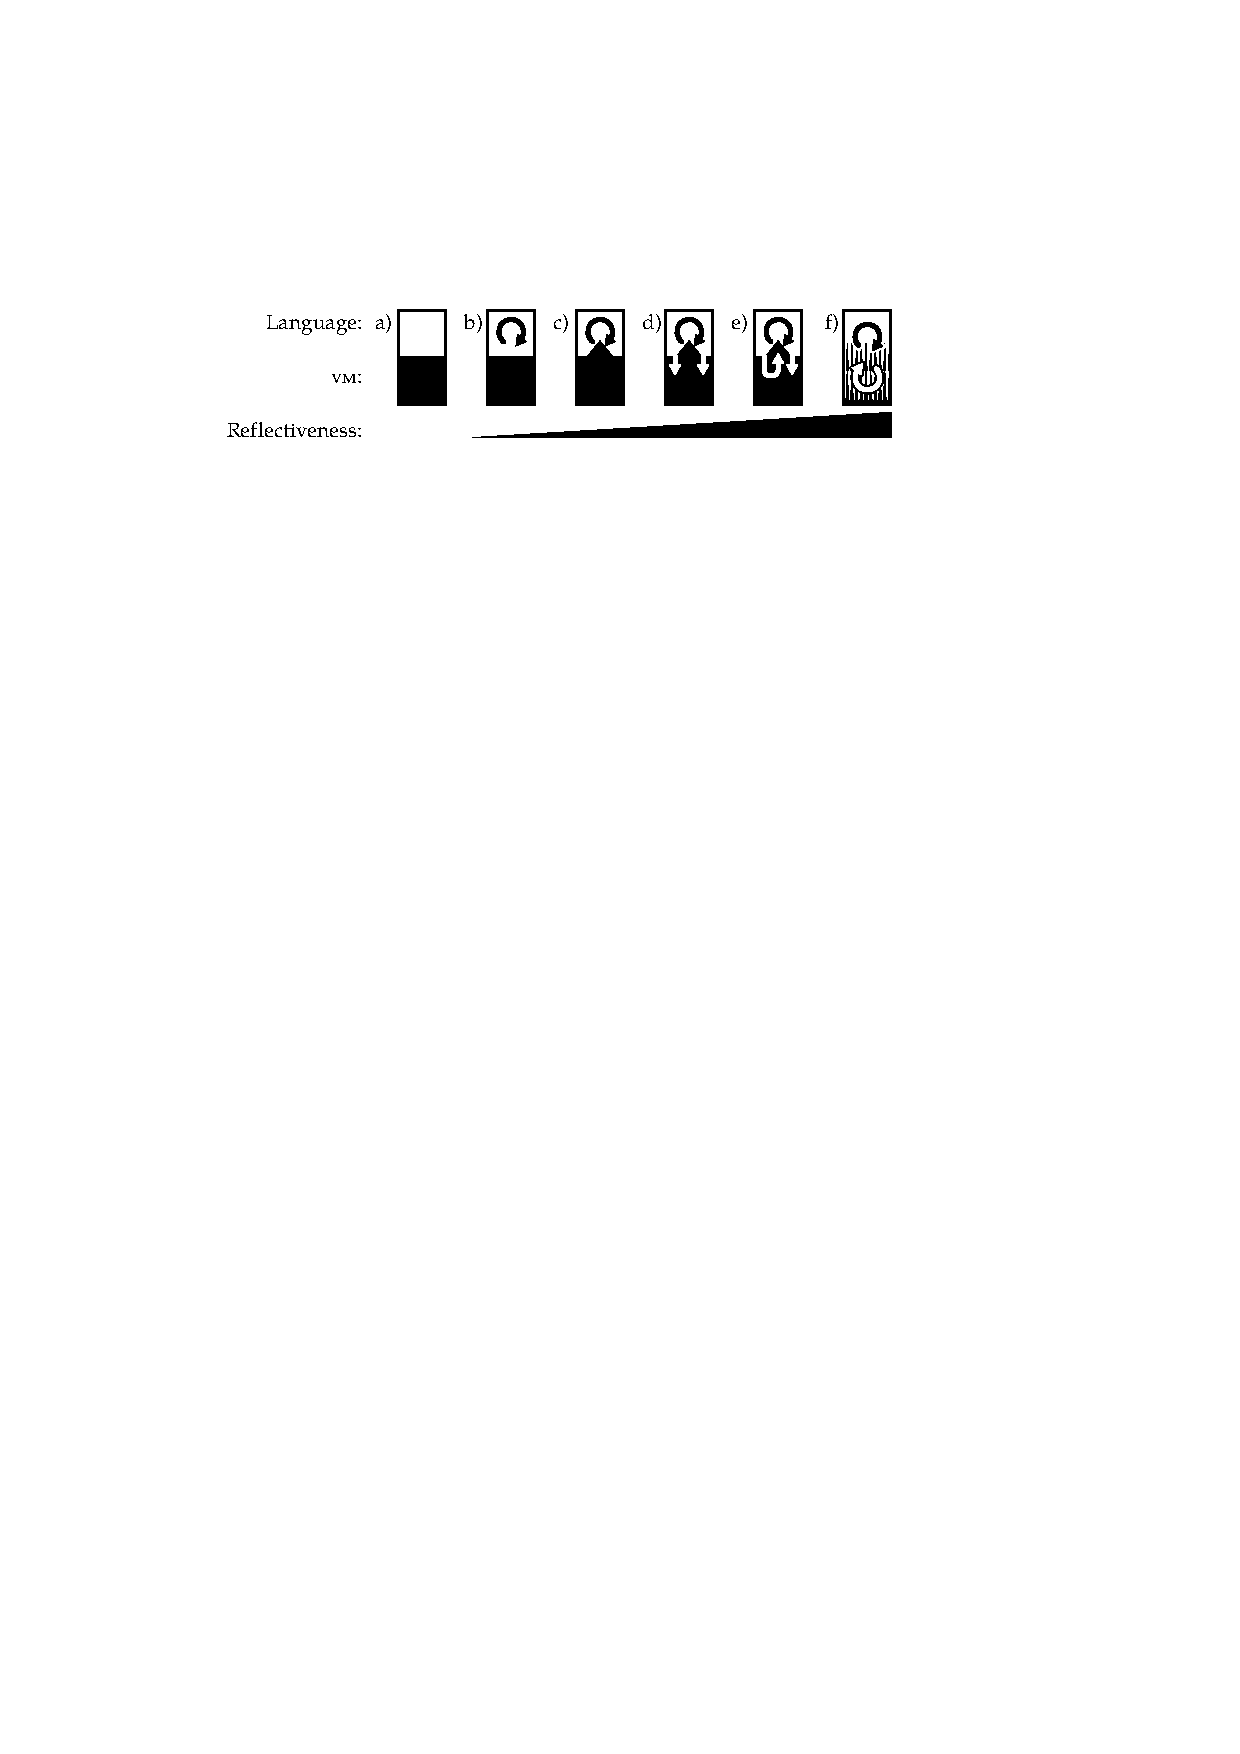
\includegraphics[scale=1.1]{vm-reflection-evolution}
\figlabel{vm-reflection-evolution}
\end{figure}
%

\begin{enumerate}[a), nolistsep]
\item \textbf{Language-side without reflection:} A language in this category requires a virtual machine to run but has no reflective properties.
	This includes early-stage languages such as the original Pascal-P system.
	Typically languages without reflection also lack the underlying \VM and are compiled directly to native code.
	\cb{thus they are one meta-level short of performing reflection}
	
\item \textbf{Language-side with limited reflection:}
	The next step is to support only certain static reflection.
	This might include structural reflection whose required information can be prepared upfront during the compilation phase.
	Such a system has no support for unanticipated reflection as there is no support from the \VM to dynamically reify concepts.
	A \VM with a \JIT in this category can perform strong optimizations and take full advantage of the runtime information.
	\cb{GO fits here? \Java only partially?}
	
\item \textbf{Language-side extended reflection:}
	The third category of high-level language runtimes has extended reflection with strong support from the underlying \VM.
	We put \PH, \ST implementations or \Self in this category of languages.
	The \VM supports complex reification of otherwise non-accessible concepts such as the stack.
	At this stage the \VM-level optimizations are a balance between restricting the supported language or sacrificing speed.
	
\item \textbf{Language-side access to the \VM:}
	The \VM support for reflection is highly extended compared to the previous category.
	Instead of a hidden property, certain \VM-level concepts are made explicitly accessible to the running language.
	Up to some extent this is similar to language-side structural reflection as the \VM only supports only a restricted interface which is defined at compile-time.
	In this category the language can only read (introspect) \VM properties.
	To our best knowledge there are no existing language-runtimes that fall into this category.

\item \textbf{Language-side modification of the \VM:}
	The previous category allows the language-side to safely read \VM-level properties.
	If we follow the same path as the language-side evolution of reflection the next step is to allow for self-modification.
	Such a language-runtime has a dynamic interface to change certain properties of the \VM.
	However, the \VM is still not fully reflective in the sense that not all \VM concepts are reified.
	This essentially limits the language-side to simple interactions and changes to the \VM itself.
	At this point the \VM can no longer guarantee safety by isolating the language-side from all the low-level details.
	Again no systems are known to fit in this category.
	
\item \textbf{Self-aware \VM:}
	We classify in the last category dynamic language-runtimes that have no longer a clear separation of \VM and language-side.
	The same reflective properties equally apply to language-side and the \VM.
	The way to achieve this is by flattening out the intermediate \VM and let the language-side directly control everything.
	Currently there are several research \VMs which can be classified as self-aware \VMs: The \P \VM \cite{Verw12a} is partially self-aware but in control of the underlying execution and the \Klein \VM is fully reflective \cite{Unga05a}. 
\end{enumerate}


\noindent From this overview of reflective evolution of high-level languages we see that there is only little research about self-aware \VMs or reflective \VMs.
In general high-level languages are built with a clear distinction of the language-side and the \VM.
However, with further reflective capabilities of the language-side we see that such a separation is no longer a guarantee for security.
In fact most security aspects have to be addressed already at language-side \cite{??}.
This we want to focus in this thesis on the reflective aspects of the \VM.


% ===========================================================================
\section{Open \VMs}
\seclabel{background-open-vms}
% ===========================================================================
\todo{Simple History of \VMs: static frames, high abstraction mismatch}\\
\todo{missign structural refleciton => go towards \VM frameworks} \\
\todo{At the same time hard requirements which can only be achieved with very low-level programming}\\

% ---------------------------------------------------------------------------
\subsection{Metacircular \VMs}
\seclabel{background-metacircular-vms}
% ---------------------------------------------------------------------------
\todo{Ultimate Goal: Run the \VM in the same language... what do we improve by that?}\\
\todo{  lesser abstraction mismatch, known tools, better debugging, faster development }\\
\todo{Image different approaches 2 axis: lanugage properties(absorbed / explicit), bootstrap (intermediate, direct)}

\paragraph{Language Property Synthesis}
\todo{Where does the implemented lanugage properties come from: managed vs. explicit}.
\todo{Eraly approaches like the \Squeak \VM have no absorption}\\
\todo{Typical \VM generation framweork, akak. facny C or C++ (mimics their final staticness while being more flexible during pre-compilation)}\\
\todo{\PyPy gives not direct access to the underlying \JIT implementation, plug and play}\\
\todo{Very high-level interface}\\
\todo{Truffle as extreme to that track: Interpreter implementation on \AST basis, not explicit bytecode interpreter (which would be typical in C)}

\paragraph{Bootstrap Process}
\todo{Early approaches use C as intermeditate representation}\\
\todo{Implies the whole GCC stack} \\
\todo{Hard to circumvent GCC's limitations => generate own native code} \\
\todo{Fluent transition from purely C based bootstrap, over C-kernel + native code to purely native code} 


% ---------------------------------------------------------------------------
\subsection{Compile-time Reified \VMs}
% ---------------------------------------------------------------------------

\subsubsection*{\Squeak \ST \VM}
\seclabel{background-squeak}
% ---------------------------------------------------------------------------
\todo{Does not absorb any properties} \\
\todo{\ST used as C template engine}

\WF is implemented in \PH which uses the \urlfootnote{\Cog \VM}{http://www.mirandabanda.org/cogblog/}, originating from the \Squeak \VM\cite{Inga97a}.
The \VM itself is written in a dialect of \ST called \Slang that is essentially limited to the functionality that can be expressed with standard C code.
\Slang serves for two purposes: a high-level C preprocessor, a interactive simulator of the \VM.
The first point has severe consequences.
\Slang basically has the same syntax as \ST but is semantically constrained to expressions that can be resolved statically at compilation or code generation time and are compatible with C.
Hence \Slang's semantics are closer to C than to \ST.
This fact is also visible in the simulator for the \VM.
If \Slang were \ST, separate parts of the \VM could be directly evaluated.
However, since \Slang is bound to C expressions, the simulator sets up a byte array as memory.
The simulated \VM then accesses this byte array as if it were the native memory.

In conclusion we see that the \PH \VM has an abstract representation of the \VM available for simulation.
This abstract representation is then used to generate C sources, already lowering the abstraction level.
After compiling the C sources the original representation of the \VM is not directly accessible anymore.
For instance, even debug symbols are usually stripped from the final binary for performance reasons.
Of course this implies that the \VM can not be changed nor directly inspected from language-side.


% ---------------------------------------------------------------------------
\subsubsection*{High-level low-level Programming in \Jikes with \MMTK}
\seclabel{background-jikes}
% ---------------------------------------------------------------------------
\todo{Image: Infrastructure Overview}

High-level low-level programming \cite{Fram09a} advocates using high-level languages for system programming.
Frampton et al. present a low-level framework packaged as \ttt{org.vmmagic}, which is used as system interface for Jikes, an experimental Java VM.
Additionally their framework is successfully used in a separate project, the memory management toolkit (\MMTK) \cite{Blac04a} which is used independently in several other projects.
The \ttt{org.vmmagic} package introduces highly controlled low-level interaction in a statically type context.
Methods have to be annotated to use low-level functionality. 

The \ttt{org.vmmagic} package is much more elaborate than \NB, notably their type system extensions allow for optimized interaction between several low-level methods.
\cb{do we need to list more what they do?}
However as we state in the introduction, it is tailored towards Java with static types.
Additionally the strong separation between low-level code and runtime does not allow for reflective extensions of the runtime.

% ---------------------------------------------------------------------------
\subsubsection*{\Maxine \Java \VM}
\seclabel{background-maxine}
% ---------------------------------------------------------------------------
\Maxine is a metacircular \Java \VM \cite{Wimm13a} focused on an efficient developer experience.
The \Maxine \VM stands out as it truly focuses on productivity and developer interaction.
\Maxine uses abstract and high-level representations of \VM-level concepts and consistently exposes them throughout the development process.
Inspectors at multiple abstraction levels are readily available while debugging, giving insights to the complete \VM state.
\Maxine provides and excellent navigation for generated native code by providing links back to language-side objects as well as other native code and symbols.

Compared to \Maxine, the \B infrastructure currently lacks the debugging tools which would enable a truly seamless interaction with the low-level world.
Namely, \B does not support low-level debugging and does not support facilities to inspect low-level native code directly.
However, \Maxine focuses on \Java, a language with inferior reflective capabilities compared to \PH.
Hence the live interaction with the \VM is only possible during the development phase and not exposed to the language-side.


\subsubsection*{\PyPy}
\seclabel{background-pypy}
% ---------------------------------------------------------------------------
\urlfootnote{\PyPy}{http://pypy.org/} is a \Python-based high-level \VM framework \cite{Rigo06a}.
\PyPy's major focus lies on an efficient metacircular \Python interpreter.
However, it has been successfully used to build \VMs for other languages including \ST \cite{Bolz08a}.
Interpreters are written in a type-inferable subset of \Python called \RPython.
The underlying \PyPy infrastructure implicitly provides memory management and \JIT compilation.

\paragraph{Provided \VM Features}
\PyPy follows a different approach from the previously presented \VM generation frameworks.
For instance, in Squeak and \Jikes the final \VM implementation is not much different from C or C++.
The programmer specifies all the components of the \VM explicitly, either by implementing them directly or using a provided library.
Compared to the more static C ans C++ these \VM generation frameworks make the compilation phase more tangible.
\ST in \Squeak or \Java in \Jikes or \Maxine fulfill the purpose of the template system in C++ or the restricted macro system in C.
For the explicit implementation part \PyPy is no different.
However, certain features for the final \VM are directly absorbed from the underlying \PyPy infrastructure.
For instance, the \JIT support or the \GC are not explicitly implemented but provided by the \PyPy framework itself.
This is a big difference to the other \VM frameworks as it allows programmers to write the \VM in a more high-level fashion.
For instance in \Squeak memory allocation, even for \VM-level objects, has to be handled in the same way as in C.
Whereas in \PyPy the garbage collection is left to the underlying infrastructure.

\paragraph{\RPython Interpretation}
At compile-time the interpretation stack for a newly implemented \VM on top of \PyPy looks as follows.
%
\begin{enumerate}
\item The final language runtime
\item The \VM written in \RPython
\item The \PyPy infrastructure (virtual compile-time \RPython interpreter)
\end{enumerate}
%
Unless in debug mode, the bottom-most layer is compiled away by exporting the \RPython sources to C.
However, before the C export step, all the compile-time reflection statements are evaluated and flattened away.
This approach allows \RPython \VMs to behave almost like standard \Python programs while still providing excellent performance in the final \VM binary.

\paragraph{High-level Tracing \JIT}
Much like the automatic memory management, \PyPy provides a tracing \JIT generator \cite{Bolz09a}.
By default the \VM programmer does not write an explicit \JIT in \PyPy.
Instead the \VM code is annotated to guide the underlying tracing \JIT generator.
This means a \VM compilation time a specific tracing \JIT is created for the given meta information.
As a result, the \JIT can track high-level loops in the final interpreted language.

\todo{in that sense maybe also add truffle}


% ---------------------------------------------------------------------------
\subsection{Runtime Reified \VMs}
\seclabel{background-reified-vms}
% ---------------------------------------------------------------------------

The \VMs presented so far have little or no self-awareness.
Typically the \VM generation frameworks only allow a high amount of reflection at \VM compile time.
This meta information is typically compiled away, similar to a C++-based \VM.
The \VM frameworks themselves behave like a static language on their own.
The final \VM artifact has no access to the underlying definition anymore.
Typically some structural meta information is available at runtime but not made available to the language running on top.

We are now going to present \VMs that behave significantly different.
These \VMs have direct control over the underlying infrastructure and most concepts
\cb{yadda yadda yadda}
\todo{need proper link from static VM to dynamic VM}\\
\todo{draw parallel to C (classical VM), vs C++ (Maxine / Jikes), Java (PyPy) vs someting like ST} \\
\todo{probably add table for comparison}\\
\todo{Proper separation \cite{Wimm12a} at compile time should make it easy to push it to dynamic/runtime}


% ------------------------------------------------------------------------------
\subsubsection*{\Pinocchio \VM}
\seclabel{background-pinocchio}

The \P \VM \cite{Verw11a} presented in \secref{background-pinocchio} is a direct predecessor of the work presented in this thesis.
The knowledge gained while participating on \P had a great influence on the development direction of \B and its applications.

Unlike \PH running on the \Cog \VM the \P research \VM has no bytecode interpreter.
The only execution base is native code which is directly generated by the language-side compiler.
At the current stage of development \P has not yet support for a separate image as in \PH.
The runtime image is currently defined by the bootstrap process where classes, objects and methods are exported into binary images and linked together with a primitive kernel to a final executable.

\paragraph{Going Native}
We took from \P that language-side native code generation is not more complex than generating bytecodes.
Instead we directly embrace the native world.
This means that in the core \P already uses many concepts that are only introduced by the \JIT in the \Cog \VM.
Hence, \P does no longer distinct between \JIT mode and interpreter mode.
Here the gain for \P are twofold: we could boost the performance of the language-runtime and simplify the design by not needing a dual compilation pipeline for the \JIT and the bytecode.

\paragraph{Going Meta}
Even so \P directly uses native code as core execution mode we avoided to directly write native code if possible.
For instance the method lookup in \Cog is statically implemented at \VM-side using \Slang.
We described in \secref{background-pinocchio} in detail how \P uses language-side code instead for the lookup.
Using the combination of low-level code to flatten out meta recursion we still have full language-side control over the lookup while maintaining good performance.

\paragraph{Missing Low-level Reification}
The most obvious shortcoming of \P was the lack of its own garbage collector.
Instead of investing time into a separate well-defined \GC \P relies on the conservative \urlfootnote{Boehm \GC}{http://www.hpl.hp.com/personal/Hans_Boehm/gc/} built for C programs.
The Boehm \GC is sufficiently fast to run \P as a prototype, however, due to its generic nature it is not as efficient as a specific \GC.
However, \P lacked the necessary reification at level of the object layout to properly implement a \GC.
All the notion about the object layout in memory are hard-coded in the compiler in several places.

\todo{no real distinction between \JIT and interpreter} \\
\todo{compiler directly generates native code} \\
\todo{simplified infrastructure} \\
\todo{lagnuage-side: lookup links back to language-side code with prefilled native code to avoid meta recursion}
\todo{missing reification for the layout (work in progress)} \\
\todo{missing reification for low-level \VM objects} \\
\todo{still used minimal C kernel for simplicity} \\
\todo{required gcc + linker for bootstrap}

% ------------------------------------------------------------------------------
\subsubsection*{\MIST a C-less \ST Implementation}
\urlfootnote{\MIST}{http://mist-project.org/} is another prototype \ST \VM that follows similar goals as the \P \VM.
It not longer uses bytecode interpreter but only relies on native code.
However, it goes one step further than \P by not relying on any C-based infrastructure.
\MIST implements its own linker to build the final executable.
And unlike \P it does not require kernel primitives written in C.
\MIST brings its own implementation to directly perform system calls from within the language.

% ------------------------------------------------------------------------------
\subsubsection*{\DwarfPython}

\todo{see \cite{Kell11a}}
\todo{History based on \Parathon + \Dwarf}\\
\todo{explain unified \VM runtime model}\\
\todo{language-runtime controls everything}\\
\todo{user for better low-level interaction}\\
\todo{shared infrastructure for \FFI callout generation}\\

% ------------------------------------------------------------------------------
\subsubsection*{\Klein \VM}
\seclabel{background-klein}
\urlfootnote{\Klein}{http://kleinvm.sourceforge.net/} is a metacircular \VM for the \Self programming language that has no separation into \VM and language \cite{Unga05a}.
The \VM is entirely written in \Self but takes the concept of metacircular beyond the compile-time.
For instance, unlike many other metacircular \VMs, including \Cog and \Squeak, \Klein does not use an intermediate low-level language to bootstrap the system.
It generates directly a binary image, much like the aforementioned \P or \MIST \VM.
However, it is important to note that the \VM-level structures and objects are not compiled away as it is usually the case.
Instead the \VM structures are represented as real \Self objects.
Hence the \Klein \VM supports true \VM-level reflection since there is only a single code base.

Additionally to the advances in reflection and metacircularity, \Klein focuses on fast compilation turnarounds to allow for a responsive development process.
Which is unlike the \Squeak \VM where a full \VM bootstrap takes a order of minutes on modern hardware.
\Klein also supports advanced mirror-based debugging tools to inspect and modify a remote \VM.

Development on the \Klein \VM seized in 2009 and left the \Klein \VM in fairly usable state.
However, up to now it lacks a proper \GC which essentially limits its real-world application.
Yet, it proved that it is possible and build a language-runtime without a proper separation of the language-side and the \VM or base-level.
From the literature presented about the \Klein project we see a strong focus on the improvements of the development tools.
The fact that the language-runtime allows \VM-level reflection to change the \VM dynamically is not directly mentioned in the literature.
While we see the practical limitations of changing the \VM at runtime we would like to open the doors to this new form of reflection.
\todo{reread paper}
\todo{Image: Infrastructure Overview}


\section{Tools Accessing the VM}
\todo{properly integrate into the rest}

\subsection*{\Quicktalk}
\Quicktalk \cite{Ball86a} follows a similar path as we do with Waterfall presented in \secref{waterfall}.
However Ballard et al. focus mostly on the performance aspect.
They achieve higher performance mostly by eliminating the bytecode dispatch overhead.
Additionally they type annotate the code for the primitive definitions to benefit from further optimizations.
\WF however, is a very lightweight approach that provides less optimization opportunities on a general code base.
\Quicktalk tries to compile generic \ST code, where Waterfall is mainly applied to single limited primitives.


\subsection*{\DTrace}
\cb{maybe remove the dtrace discussion from here and move it into the waterfall section and cite \cite{Cant04a} there}
\todo{see \cite{Cant04a}}


% ===========================================================================
\section{Problem 1: }
% ===========================================================================


% ===========================================================================
\section{Problem 2: }
% ===========================================================================


% ===========================================================================
\section{Problem 3: }
% ===========================================================================


% ===========================================================================
\section{Summary and Outlook}
% ===========================================================================

\todo{Intro + List again the problems} \\
\todo{Sync Chapter Outlook}


% =============================================================================
% empty version for the main document, where all the chapters are compiled together
%\documentclass[a4paper,10pt,twoside]{../includes/ThesisStyle}
\usepackage[utf8]{inputenc}
\usepackage[T1]{fontenc}

\usepackage[left=1.5in,right=1.3in,top=1.1in,bottom=1.1in,includefoot,includehead,headheight=13.6pt]{geometry}\renewcommand{\baselinestretch}{1.05}


% =============================================================================
%\usepackage[sectionbib]{chapterbib}	% Cross-reference package (Natural BiB)
%\usepackage{bibunits}
%\usepackage{natbib}					% Put References at the end of each chapter
\usepackage{algorithm}
\usepackage{alltt}
\usepackage{amsfonts}
\usepackage{amsmath}
\usepackage{amssymb}
\usepackage{cite}
\usepackage{color}
\usepackage{enumerate}
\usepackage{fancyhdr}					% Fancy Header and Footer
\usepackage{graphicx}
\usepackage{ifthen}
\usepackage{latexsym}
\usepackage{multirow}
\usepackage{rotating}					% Sideways of figures & tables
\usepackage{stmaryrd}
\usepackage{subfigure}
\usepackage{url}         
\usepackage{xspace}

\usepackage[a4paper,pagebackref,hyperindex=true]{hyperref}
        

% =============================================================================

% Table of contents for each chapter
\usepackage[nottoc, notlof, notlot]{tocbibind}
\usepackage{minitoc}
\setcounter{minitocdepth}{1}
\mtcindent=15pt

\setcounter{secnumdepth}{3}
\setcounter{tocdepth}{2}
  
% =============================================================================
% Fancy Header Style Options

\pagestyle{fancy}                       % Sets fancy header and footer
\fancyfoot{}                            % Delete current footer settings

%\renewcommand{\chaptermark}[1]{         % Lower Case Chapter marker style
%  \markboth{\chaptername\ \thechapter.\ #1}}{}} %

%\renewcommand{\sectionmark}[1]{         % Lower case Section marker style
%  \markright{\thesection.\ #1}}         %

\fancyhead[LE,RO]{\bfseries\thepage}    % Page number (boldface) in left on even
% pages and right on odd pages
\fancyhead[RE]{\bfseries\nouppercase{\leftmark}}      % Chapter in the right on even pages
\fancyhead[LO]{\bfseries\nouppercase{\rightmark}}     % Section in the left on odd pages

\let\headruleORIG\headrule
\renewcommand{\headrule}{\color{black} \headruleORIG}
\renewcommand{\headrulewidth}{1.0pt}
\usepackage{colortbl}
\arrayrulecolor{black}

\fancypagestyle{plain}{
  \fancyhead{}
  \fancyfoot{}
  \renewcommand{\headrulewidth}{0pt}
}


% =============================================================================
% Clear Header Style on the Last Empty Odd pages
\makeatletter

\def\cleardoublepage{\clearpage\if@twoside \ifodd\c@page\else%
  \hbox{}%
  \thispagestyle{empty}%              % Empty header styles
  \newpage%
  \if@twocolumn\hbox{}\newpage\fi\fi\fi}

\makeatother

\newenvironment{maxime}[1]
{
\vspace*{0cm}
\hfill
\begin{minipage}{0.5\textwidth}%
%\rule[0.5ex]{\textwidth}{0.1mm}\\%
\hrulefill $\:$ {\bf #1}\\
%\vspace*{-0.25cm}
\it 
}%
{%

\hrulefill
\vspace*{0.5cm}%
\end{minipage}
}

\let\minitocORIG\minitoc
\renewcommand{\minitoc}{\minitocORIG \vspace{1.5em}}


\renewcommand{\epsilon}{\varepsilon}

% centered page environment
\newenvironment{vcenterpage}
	{\newpage\vspace*{\fill}\thispagestyle{empty}\renewcommand{\headrulewidth}{0pt}}
	{\vspace*{\fill}}
	
	
% =============================================================================
\newboolean{showcomments}
\setboolean{showcomments}{true}

\ifthenelse{\boolean{showcomments}} {
	\newcommand{\ugh}[1] {\textcolor{red}{\uwave{#1}}}	% please rephrase
	\newcommand{\ins}[1] {\textcolor{blue}{\uline{#1}}}	% please insert
	\newcommand{\del}[1] {\textcolor{red}{\sout{#1}}}	% please delete
	\newcommand{\chg}[2] {								% please change
		\textcolor{red}{\sout{#1}}{\ra}
		\textcolor{blue}{\uline{#2}}}
	\newcommand{\nbc}[3]{								% comment
		{\colorbox{#3}{\bfseries\sffamily\scriptsize\textcolor{white}{#1}}}
		{\textcolor{#3}{\sf\small$\blacktriangleright$\textit{#2}$\blacktriangleleft$}}}

}{
	\newcommand{\ugh}[1]{#1}							% please rephrase
	\newcommand{\ins}[1]{#1}							% please insert
	\newcommand{\del}[1]{}								% please delete
	\newcommand{\chg}[2]{#2}							% please change
	\newcommand{\nbc}[3]{}								% comment
}

% =============================================================================
\usepackage[a4paper,pagebackref,hyperindex=true]{hyperref}


% Links in pdf
\usepackage{color}
\definecolor{linkcol}{rgb}{0.0, 0.0, 0.0} 
\definecolor{citecol}{rgb}{0.0, 0.0, 0.0} 

% Change this to change the informations included in the pdf file
% See hyperref documentation for information on those parameters
\hypersetup {
	bookmarksopen=true,
	pdftitle="Design and Use of Anatomical Atlases for Radiotherapy",
	pdfauthor="Olivier COMMOWICK", 
	pdfsubject="Creation of atlases and atlas based segmentation", %subject of the document
	%pdftoolbar=false, % toolbar hidden
	pdfmenubar=true, %menubar shown
	pdfhighlight=/O, %effect of clicking on a link
	colorlinks=true,
	pdfpagemode=None,
	pdfpagelayout=SinglePage,
	pdffitwindow=true,
	linkcolor=linkcol,
	citecolor=citecol,
	urlcolor=linkcol
}

% =============================================================================
\newcommand{\figlabel}[1]{\label{fig:#1}}
\newcommand{\seclabel}[1]{\label{sec:#1}}
\newcommand{\tablabel}[1]{\label{tab:#1}}

\newcommand{\figref}[1]{Figure~\ref{fig:#1}}
\newcommand{\secref}[1]{Section~\ref{sec:#1}}
\newcommand{\tabref}[1]{Table~\ref{tab:#1}}

\newcommand{\commented}[1]{}

\newcommand{\eg}{\emph{e.g.,}\xspace}
\newcommand{\ie}{\emph{i.e.,}\xspace}


\newcommand\fix[1]{\nb{FIX}{#1}}
\newcommand\todo[1]{\nb{TO DO}{#1}}

% =============================================================================

\graphicspath{{.}{../figures/}}

\begin{document}
% =============================================================================
\chapter{Reification}
\chaplabel{reification}
\minitoc
% =============================================================================

% =============================================================================
\section{Introduction}
% =============================================================================





% =============================================================================
\section{Simple Language-side Reification}
% =============================================================================

% VM objects
% OS Environment Objects



% =============================================================================
\section{Inspectors: Visual Reification}
% =============================================================================


% ---------------------------------------------------------------------------
\subsection{The Inspector Model}
% ---------------------------------------------------------------------------


% ---------------------------------------------------------------------------
\subsection{Inspector Applications}
% ---------------------------------------------------------------------------


% =============================================================================
\section{First-class Object Layouts: Bridging the Gap to the Memory}
% =============================================================================

% ---------------------------------------------------------------------------
\subsection{Objects All the Way}
% ---------------------------------------------------------------------------


% ---------------------------------------------------------------------------
\subsection{Layouts and Slots}
% ---------------------------------------------------------------------------


% ---------------------------------------------------------------------------
\subsection{Future Applications}
% ---------------------------------------------------------------------------


% =============================================================================
\section{Related Work}
% =============================================================================

% -----------------------------------------------------------------------------
\subsection{Meta Object Protocols}
% -----------------------------------------------------------------------------


% -----------------------------------------------------------------------------
\subsection{VM Hooks}
% -----------------------------------------------------------------------------

% standard smalltalk hooks: DNU and so forth
% inline cache hook in Smalltalk/X?



% =============================================================================
\section{Summary}
% =============================================================================


% =============================================================================
% empty version for the main document, where all the chapters are compiled together
% =============================================================================
\documentclass[a4paper,10pt,twoside]{../includes/ThesisStyle}
\usepackage[utf8]{inputenc}
\usepackage[T1]{fontenc}

\usepackage[left=1.5in,right=1.3in,top=1.1in,bottom=1.1in,includefoot,includehead,headheight=13.6pt]{geometry}\renewcommand{\baselinestretch}{1.05}


% =============================================================================
%\usepackage[sectionbib]{chapterbib}	% Cross-reference package (Natural BiB)
%\usepackage{bibunits}
%\usepackage{natbib}					% Put References at the end of each chapter
\usepackage{algorithm}
\usepackage{alltt}
\usepackage{amsfonts}
\usepackage{amsmath}
\usepackage{amssymb}
\usepackage{cite}
\usepackage{color}
\usepackage{enumerate}
\usepackage{fancyhdr}					% Fancy Header and Footer
\usepackage{graphicx}
\usepackage{ifthen}
\usepackage{latexsym}
\usepackage{multirow}
\usepackage{rotating}					% Sideways of figures & tables
\usepackage{stmaryrd}
\usepackage{subfigure}
\usepackage{url}         
\usepackage{xspace}

\usepackage[a4paper,pagebackref,hyperindex=true]{hyperref}
        

% =============================================================================

% Table of contents for each chapter
\usepackage[nottoc, notlof, notlot]{tocbibind}
\usepackage{minitoc}
\setcounter{minitocdepth}{1}
\mtcindent=15pt

\setcounter{secnumdepth}{3}
\setcounter{tocdepth}{2}
  
% =============================================================================
% Fancy Header Style Options

\pagestyle{fancy}                       % Sets fancy header and footer
\fancyfoot{}                            % Delete current footer settings

%\renewcommand{\chaptermark}[1]{         % Lower Case Chapter marker style
%  \markboth{\chaptername\ \thechapter.\ #1}}{}} %

%\renewcommand{\sectionmark}[1]{         % Lower case Section marker style
%  \markright{\thesection.\ #1}}         %

\fancyhead[LE,RO]{\bfseries\thepage}    % Page number (boldface) in left on even
% pages and right on odd pages
\fancyhead[RE]{\bfseries\nouppercase{\leftmark}}      % Chapter in the right on even pages
\fancyhead[LO]{\bfseries\nouppercase{\rightmark}}     % Section in the left on odd pages

\let\headruleORIG\headrule
\renewcommand{\headrule}{\color{black} \headruleORIG}
\renewcommand{\headrulewidth}{1.0pt}
\usepackage{colortbl}
\arrayrulecolor{black}

\fancypagestyle{plain}{
  \fancyhead{}
  \fancyfoot{}
  \renewcommand{\headrulewidth}{0pt}
}


% =============================================================================
% Clear Header Style on the Last Empty Odd pages
\makeatletter

\def\cleardoublepage{\clearpage\if@twoside \ifodd\c@page\else%
  \hbox{}%
  \thispagestyle{empty}%              % Empty header styles
  \newpage%
  \if@twocolumn\hbox{}\newpage\fi\fi\fi}

\makeatother

\newenvironment{maxime}[1]
{
\vspace*{0cm}
\hfill
\begin{minipage}{0.5\textwidth}%
%\rule[0.5ex]{\textwidth}{0.1mm}\\%
\hrulefill $\:$ {\bf #1}\\
%\vspace*{-0.25cm}
\it 
}%
{%

\hrulefill
\vspace*{0.5cm}%
\end{minipage}
}

\let\minitocORIG\minitoc
\renewcommand{\minitoc}{\minitocORIG \vspace{1.5em}}


\renewcommand{\epsilon}{\varepsilon}

% centered page environment
\newenvironment{vcenterpage}
	{\newpage\vspace*{\fill}\thispagestyle{empty}\renewcommand{\headrulewidth}{0pt}}
	{\vspace*{\fill}}
	
	
% =============================================================================
\newboolean{showcomments}
\setboolean{showcomments}{true}

\ifthenelse{\boolean{showcomments}} {
	\newcommand{\ugh}[1] {\textcolor{red}{\uwave{#1}}}	% please rephrase
	\newcommand{\ins}[1] {\textcolor{blue}{\uline{#1}}}	% please insert
	\newcommand{\del}[1] {\textcolor{red}{\sout{#1}}}	% please delete
	\newcommand{\chg}[2] {								% please change
		\textcolor{red}{\sout{#1}}{\ra}
		\textcolor{blue}{\uline{#2}}}
	\newcommand{\nbc}[3]{								% comment
		{\colorbox{#3}{\bfseries\sffamily\scriptsize\textcolor{white}{#1}}}
		{\textcolor{#3}{\sf\small$\blacktriangleright$\textit{#2}$\blacktriangleleft$}}}

}{
	\newcommand{\ugh}[1]{#1}							% please rephrase
	\newcommand{\ins}[1]{#1}							% please insert
	\newcommand{\del}[1]{}								% please delete
	\newcommand{\chg}[2]{#2}							% please change
	\newcommand{\nbc}[3]{}								% comment
}

% =============================================================================
\usepackage[a4paper,pagebackref,hyperindex=true]{hyperref}


% Links in pdf
\usepackage{color}
\definecolor{linkcol}{rgb}{0.0, 0.0, 0.0} 
\definecolor{citecol}{rgb}{0.0, 0.0, 0.0} 

% Change this to change the informations included in the pdf file
% See hyperref documentation for information on those parameters
\hypersetup {
	bookmarksopen=true,
	pdftitle="Design and Use of Anatomical Atlases for Radiotherapy",
	pdfauthor="Olivier COMMOWICK", 
	pdfsubject="Creation of atlases and atlas based segmentation", %subject of the document
	%pdftoolbar=false, % toolbar hidden
	pdfmenubar=true, %menubar shown
	pdfhighlight=/O, %effect of clicking on a link
	colorlinks=true,
	pdfpagemode=None,
	pdfpagelayout=SinglePage,
	pdffitwindow=true,
	linkcolor=linkcol,
	citecolor=citecol,
	urlcolor=linkcol
}

% =============================================================================
\newcommand{\figlabel}[1]{\label{fig:#1}}
\newcommand{\seclabel}[1]{\label{sec:#1}}
\newcommand{\tablabel}[1]{\label{tab:#1}}

\newcommand{\figref}[1]{Figure~\ref{fig:#1}}
\newcommand{\secref}[1]{Section~\ref{sec:#1}}
\newcommand{\tabref}[1]{Table~\ref{tab:#1}}

\newcommand{\commented}[1]{}

\newcommand{\eg}{\emph{e.g.,}\xspace}
\newcommand{\ie}{\emph{i.e.,}\xspace}


\newcommand\fix[1]{\nb{FIX}{#1}}
\newcommand\todo[1]{\nb{TO DO}{#1}}

% =============================================================================

\graphicspath{{.}{../figures/}}

\begin{document}
% ===========================================================================
\chapter{\B: Low-level Glue in \PH}
\chaplabel{benzo}
\minitoc
% ===========================================================================
\introduction
% ===========================================================================

\sm{For me, this is not an artefact show, it is a thesis, so, I would expect to read something relating the artifact to the problem statement, and using precise terminology as devised in sec. 2}

In this chapter we present \B a framework that connects the low-level \VM world with a reflective and dynamic language-side library.
Unlike more classical approaches \B does not resort to vast set of customized \VM primitives or plugins.
\sm{Do you really want to talk about  1 generic vs. many specific things that are exposed to facilitate low level programming? I would think the point you are trying to make here conflates again multiple aspects. Take the things apart, and make one argument at a time

I see at least the question of the VM interface here, and then the question how low level functionality is provided, that's two very different things}
Instead it relies on a generic primitive to activated native code that is generated at language-side.

\B provides a unique experience of being extremely low-level yet using high-level concepts at the same time.
\sm{Bla Bla, you are not saying anything here}
This is possible since the framework is implemented at language-side and tightly integrated into the \PH development environment.
In this chapter we present in detail how \B interacts with \PH and what the difficulties are.
The key components of \B are:
\begin{itemize}[noitemsep]
	\item A generic primitive to activate native code
	\item \AsmJIT A language-side assembler
	\item A language-side library for installing and activating native code
\end{itemize}
\sm{Don't Bla Bla, be specific from the start, perhaps in more general terms, but not just with empty phrases: native code activation, native code generation, all on the language level}

\noindent Based on \B we outline 3 unique applications in \secref{benzo-usecase}:
\begin{itemize}[noitemsep]
	\item Foreign Function Interfaces (in more detail in \chapref{ffi})
	\item Dynamic Primitives (in more detail in  \chapref{validation})
	\item Language-side \JIT (in more detail in  \chapref{validation})
\end{itemize}


% ===========================================================================
\section{Background}
\seclabel{benzo-background}
% ===========================================================================
\sd{Maybe you need a stronger analysis in a previous chapter}
High-level low-level programming \cite{Fram09a} encourages to use high-level languages such as \Java to build low-level execution infrastructures or to do system programming. 
It is successfully used in experimental high-level self-hosted virtual machines (\VMs) such as \Jikes~\cite{Alpe99a}.  
Frampton et al. present a framework that is biased towards a statically typed high-level language, taking strict security aspects into account.
Their approach promotes to address low-level system programming tasks with the tools and abstractions of high-level languages.
However, their solution has reduced applicability in a dynamic and reflective context.
By reflective, we refer to the combined capabilities to inspect (introspection) and change (intercession) the same execution concepts at runtime \cite{Maes87a}.
\sm{No place for definitions, back ref to sec 2. At most.}

From a reflective point of view it seems natural to dynamically modify the \VM at runtime and not just at compile-time.
If we are able to modify the \VM from language-side we blur the line between these two distinct worlds, becoming indistinguishable to talk about the \VM or the language-side.
Hence throughout this chapter we use the term language runtime to refer to the running \VM combined with the language-side application.
\sm{Be very careful with your language, and the aspect that is novel to your approach, you don't want to imply false}


% ---------------------------------------------------------------------------
\subsection{Requirements}
% ---------------------------------------------------------------------------

Extending the \VM is only one particular case of modifying or extending the complete language runtime.
Language-side libraries, reflective capabilities, \VM extensions or hybrid approaches are other possibilities which we discuss in detail in \secref{benzo-related}.
All these typical extension mechanisms are not sufficient if we want to modify the \VM from language-side, or in our terminology, to reflectively modify the language runtime. Furthermore these mechanisms are based on the fact that there is a clear barrier between language and \VM.
A solution that crosses these barriers requires the following properties:

\begin{enumerate}
	\item It must be \emph{reflective} in the sense it must support \emph{dynamic} changes of the language runtime (\VM) without requiring a system restart.
	\item It should imply minimal changes to the existing low-level runtime to \emph{considerably reduce development efforts}.
	\sm{Should only be a recap of previously stated thesis goals}
\end{enumerate}


% ---------------------------------------------------------------------------
\subsection{\B a Framework for Reflective Low-level Programming}
% ---------------------------------------------------------------------------

\sd{repetition with below}
High-level low-level programming is a powerful technique for system programming without resorting to static low-level environments \cite{Fram09a,Wimm13a} that almost fulfills our requirements.
However, in a reflective setup it fails to comply with the first requirement mentioned in the previous paragraph: it does not allow reflective changes at runtime.
\sm{See limitations should be made very clear and referencable in chapter 2, and here you should reference them again.}
Our approach for overcoming this limitation consists of \B, a lightweight and reflective framework that dynamically generates native code from language-side and allows its execution on the fly.
It relies only on a small set of generic \VM extensions described in \secref{benzo-vm-requirements}, whereas the vast majority of the framework is implemented as a language-side library.

% ---------------------------------------------------------------------------
\subsection{\B Applications}
% ---------------------------------------------------------------------------
In \secref{benzo-usecase} we advocate the contribution of \B by providing three different incremental examples that heavily use the framework.
Unlike typical implementations that would focus on writing them as \VM extensions, we implement them completely at language-side using \B:
\sm{I think, here your structure of the thesis breaks down. After intro and related work, I would do a requirements chapter (perhaps part of 2), and then, this chapter here would be a conceptual analysis of the problem, and the proposal of the solution. (What's the minimal solution to make a VM self-aware? Explain the problems, reason about designs, and justify the choice of a 'one primitive to activates native code' solution (I guess, plus high level representation of concepts in terms of language side frameworks) then, afterwards, you can split out the discussion of benzo as your specific experiment, and all the validation is nicely separated in their respective }

\begin{description}
	\item[Language-side \FFI] A complete language-side Foreign Function Interface (\FFI) implementation, described in \secref{benzo-ffi} and in more detail in \chapref{ffi}.
	\item[Dynamic Primitives] A language-side compilation toolchain that replaces system primitives at runtime with customized code, described later in \secref{benzo-waterfall} and in more detail in \secref{val-waterfall}. 
	\item[Language-side \JIT Compiler] A \JIT compiler that works at language-side and interacts with the \VM for code synchronization, described in \secref{benzo-nabujito} and in more detail in \secref{val-nabujito}.
\end{description}

\noindent Illustrated by these three distinct examples, the contributions of this chapter are:
\begin{enumerate} 
	\item A \emph{reflective} high-level low-level programming framework that encourages the extension of high-level language runtimes on the fly without the overheads imposed by pure high-level solutions. 
	\item A proof of concept of the proposal with the implementation and description of three different tools that heavily use reflective low-level programming and covers distinct scenarios.
\end{enumerate}

% ===========================================================================
\section{The \B Framework}
\seclabel{benzo-benzo}
% ===========================================================================
\B is implemented in \urlfootnote{\PH}{http://pharo.org/}\sm{You introduced Pharo before as your platform, no?}, a \ST inspired language.
\PH comes with all the reflective capabilities known from \ST where most lan\-guage-side components can be altered dynamically.
\B is implemented at lan\-guage-side and only requires the help of two simple and generic primitives to activate native code and resolve the entry point address position of referenced C functions.

%----------------------------------------------------------------------------
\subsection{\VM Context}
\seclabel{benzo-vm-requirements}
%----------------------------------------------------------------------------
\sm{Him, I would have put all that into a separated thing, all the technical details, assumptions, and considerations }
\PH emerged from the Squeak project \cite{Inga97a}.
The \PH \VM (Cog) implementation \cite{Mira11a} also evolved from the original Squeak bytecode interpreter.
The current \VM uses a moving Garbage Collector (\GC) with two generations and uses a \JIT that applies basic register allocation to reduce stack load. 
This situation is not a direct requirement for \B but it is assumed as given and thus not further discussed in detail.
However, \B requires certain features that were not supported in the existing implementation of the \Cog \VM.
Mainly our requirement is being able to generate executable code and activate it at runtime.
This is general and essential so it applies to any \VM that wants to support dynamic code execution managed at language-side.
\sm{This is not novel, I would guess, the overall story, perhaps with minimalism as a property should probably be the selling point, so, make clear that this is existing stuff, and not part of he contribution you claim}

%----------------------------------------------------------------------------
\paragraph{Executable Memory}
\seclabel{benzo-exeutable-memory}
 
We chose to follow a very lightweight approach to dynamically execute native code at runtime. 
Since we use \PH as our host language it is a natural choice to manage the native code at language-side and use as few \VM features as possible.
Hence we use normal \PH objects to hold the generated native code.
\sm{This is your thesis goal, no? Motivate it like that, don't just put it here as incidental!}

However, by default the object memory is not executable.
This leaves two choices, either mark the whole object memory executable or move the objects with the native code to a special executable memory region.
We took the \ugh{path of least resistance} and marked the whole object memory as executable.
\sm{This argumentation is problematic, need to have a better argument, relate decision to thesis goals and scope, security is no concern, or something like that.

Might also be better discussed in alter discussion and limitation section instead, here it's mostly distracting}
The other solution requires substantial changes for memory management. 

The \GC of the \PH \VM uses a moving semi-space approach with two generations.
Additionally there is a fixed sized executable region used for the \JIT as a buffer for runtime generated native code.
The \JIT space uses its own small garbage collection strategy which is decoupled from the rest of the object memory.
This also means that the \JIT space does not hold normal \PH objects but special low-level structures.
As mentioned before, the \JIT space is limited in size and eventually fills up, causing the \JIT to spill older code structures from there. 

The \JIT-space is built for holding native code objects.
However, since the \JIT objects are volatile this is not the place to keep long-living language-side objects holding native code.
Instead we opt for the completely executable object memory option and store all the executable code in standard \PH objects.
As the \VM has a moving \GC, it gives us certain restrictions on what kind of native code we can run directly from the language-side. 
As we will describe in \secref{benzo-platform-interaction}, we can access high-level \PH objects only via an indirection from low-level code.
\sm{Come on, be a little creative, this is the obvious design decision derived from your vision and thesis goals, no discussion, just stating it here, discussion goes into the discussion section}

%----------------------------------------------------------------------------
\paragraph{\VM Interaction}
\seclabel{benzo-vm-interaction}

The standard way in \PH to execute low-level code is to use a tag in the method definition.
The following example shows the multiplication method on the \ttt{Float} class.
%
\begin{stcode}[label={lst:benzo-basic-primitive}]{5}
* aNumber 
	<primitive: 49>
	^ aNumber adaptToFloat: self andSend: #*
\end{stcode}
%
Here we use the primitive 49 to call a \VM function which efficiently multiplies two floats. 
\figref{benzo-smalltalkPrimitive}-a describes the case where the primitive is successfully executed.
However, if the primitive is unable to do the operation, for instance if the argument \ttt{aNumber} is not a float, it will signal a failure which causes the \VM to execute the fallback \PH code in the method body.  
\figref{benzo-smalltalkPrimitive}-b describes it. 
In the floating point multiplication example the fallback code uses a slow conversion method to polymorphically convert other objects to floats and defer the multiplication.


\begin{figure}[ht]
	\centering
	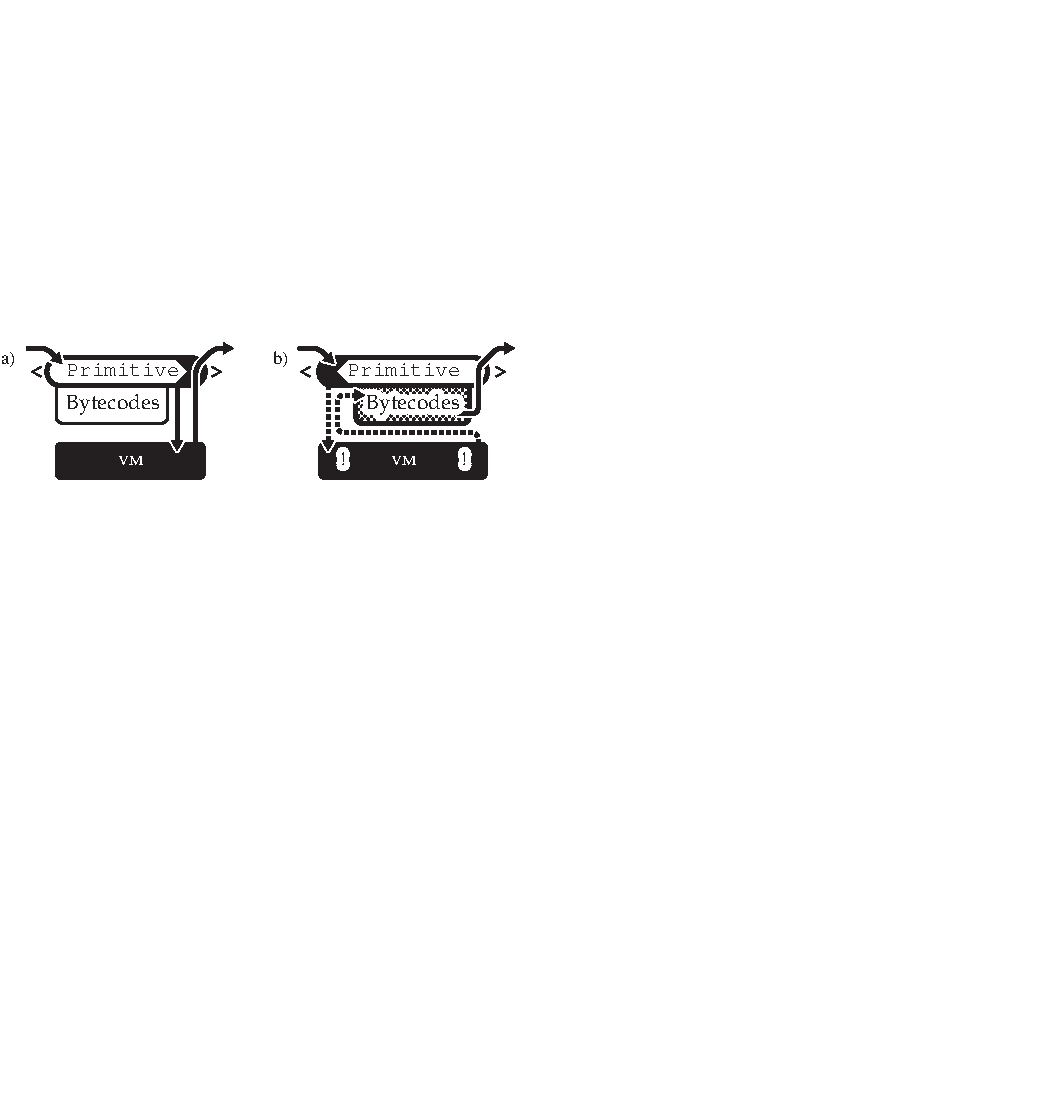
\includegraphics[scale=\imagescale]{smalltalkPrimitive}
	\caption[\PH Primitive]{Generic primitive methods in \PH: a) A primitive completely bypasses the bytecode, b) A failing primitive executes the bytecode as fallback.}
	\figlabel{benzo-smalltalkPrimitive}
\end{figure}

\noindent \B uses the primitives as a gate to enter the low-level world from the language-side.
Our custom primitive then executes the generated native code and returns to language-side. 
This code is appended inside the compiled method object.
When the primitive is activated, it  accesses the currently executed compiled method via a \VM function. 
\figref{benzo-nativeCodeMethod} shows the structure of a \PH compiled method that has native code attached to it.
We see the primitive tag on top, followed by the literal frame which holds references to symbols and classes used in the method.
The subsequent \PH bytecode is the fallback code executed only if the primitive fails. Only then appears the native instructions.
A marker at the end of the compiled method called trailer type is used to flag methods that actually have native code attached to them.
%
\begin{figure}[ht]
	\centering
	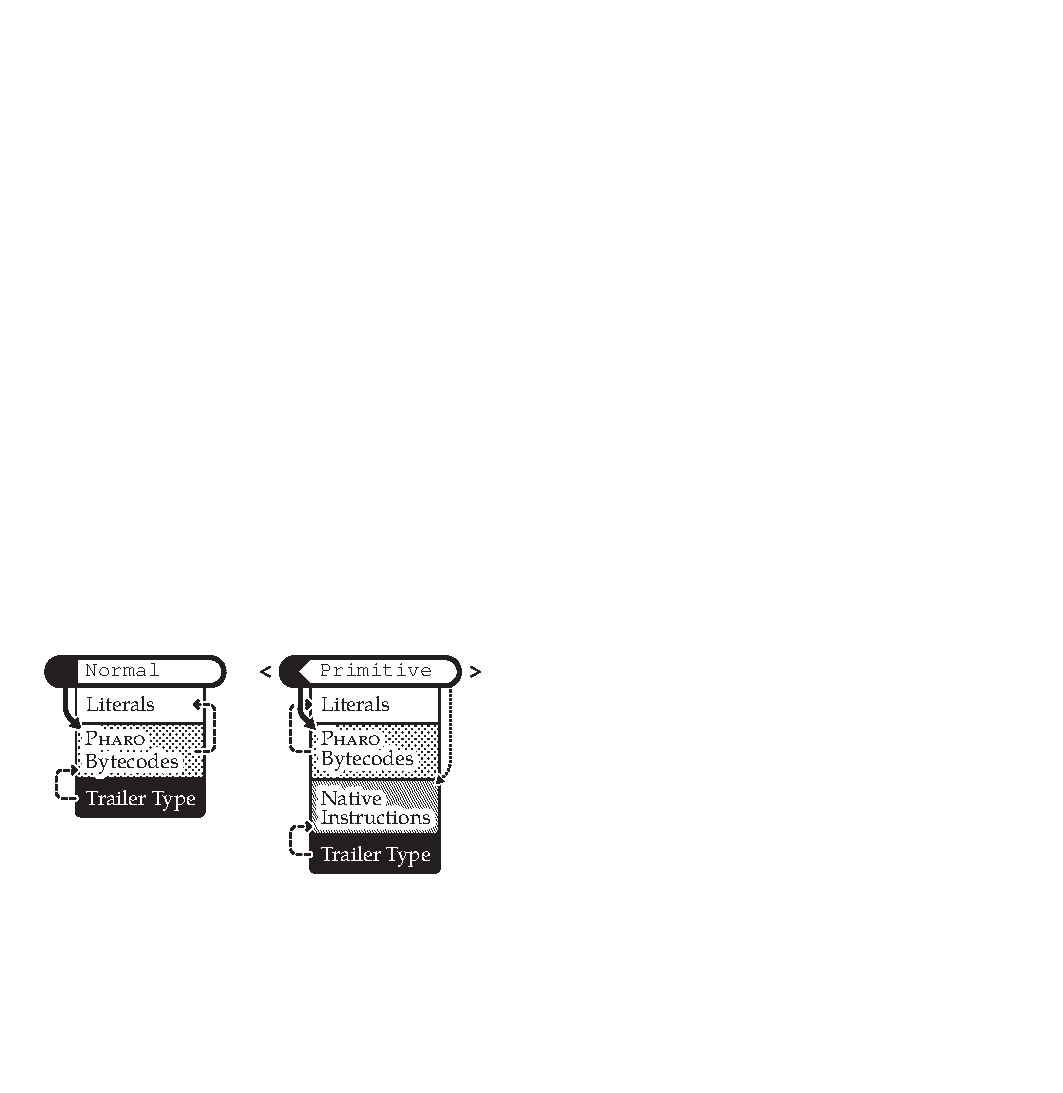
\includegraphics[scale=\imagescale]{nativeCodeMethod}
	\caption[\PH Compiled Method]{A standard \PH compiled method on the left and a method with appended native instructions generated by \B.}
	\figlabel{benzo-nativeCodeMethod}
\end{figure}

\noindent Since compiled methods are first-class objects it is possible to modify them at runtime and append the native code.
The primitive \ttt{primitiveNativeCall}, which is implemented by \B, is the responsible of running the native instructions in a \PH method.
The code example \ttt{interrupt3} shows a very basic application of our infrastructure.
\sm{Interrupt 3, really? That's the best name? You could also tell me that it is the standard interrupt for debuggers}
%
\begin{stcode}[label={lst:benzo-basic-native-code}, caption={\PH method using \B for very basic low-level debugging.}, escapeinside={@}{@}]{5}
interrupt3
	<primitive: 'primitiveNativeCall' 
	 module: 'Benzo' >
	Benzo generate: [ :asm | asm int3 ]
\end{stcode}
%
The primitive named \ttt{primitiveNativeCall} on the first line tries to run the native instructions appended to the compiled method.
When there is no native code yet the primitive fails and on return it evaluate the rest of the \PH code in the method.
In \secref{benzo-language-side}, through more detailed examples, we describe how \B uses \PH code to generate the native instructions
\figref{nativeCodeMethodDetail} shows the resulting compiled method in full detail.
%
\begin{figure}[ht]
    \centering
    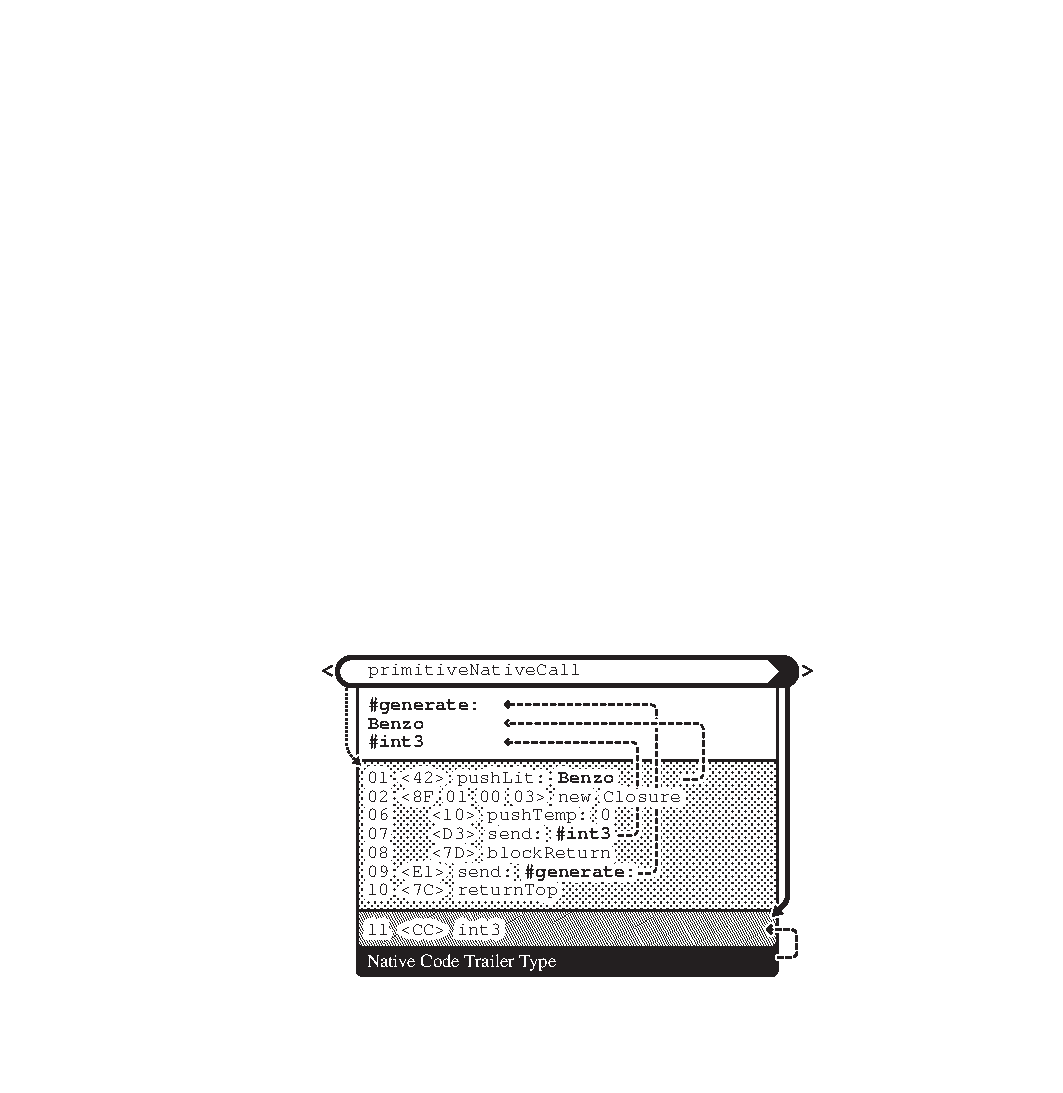
\includegraphics[scale=\imagescale]{nativeCodeMethodDetail}
    \caption[\ttt{CompiledMethod} With \B Code]{Example of \PH method with native code which calls the low-level debug exception handler \ttt{INT3}. The bytecode references objects indirectly via the literal frame residing at the beginning of the method.}
    \figlabel{nativeCodeMethodDetail}
\end{figure}

%----------------------------------------------------------------------------
\paragraph{Native Code Platform Interaction}
\seclabel{benzo-platform-interaction}

To ensure that the code is compatible with the current platform a \VM specific marker is expected at the beginning of the native code on the compiled method.
Upon activation \B compares this marker with the one from the current \VM.
If they do not match, \B signals a failure that causes the \VM to evaluate the fallback \PH code.
With this elegant approach \B regenerates native code lazily on new platforms.
Moreover, it does not have to flush the native code when the application is restarted on the same platform.
\sm{Reexecute vs. restart}

%----------------------------------------------------------------------------
\paragraph{Garbage Collector Interaction}
\seclabel{benzo-gc-interaction}
\seclabel{benzo-external-roots}

Compiled methods in \PH have a special section, the literal frame, which stores objects referenced in the bytecodes.
\sm{Did you introduce compiled methods as representing smalltalk methods? Because you use it in a way that's only unambiguous if you are a smalltalker}
Bytecodes then only have indirect access to these objects by indexing into the literal frame.
This simplifies the implementation of the garbage collector as it only has to scan the beginning of each method for possible references to objects. 
So the \GC only tracks \PH objects when they are in the method literal frame. 
The moving \GC of the \VM used for \PH has a significant impact on the low-level code we can generate using \B.
For instance it is not possible to statically refer to language-side objects from native code as object addresses change after each garbage collection.
Modifying the \GC to support regions of non-moving objects would solve this problem.
However, we chose to minimize the number of low-level \VM modification necessary to run our experiments and opted for a simpler solution.

\begin{figure}[ht]
	\centering
	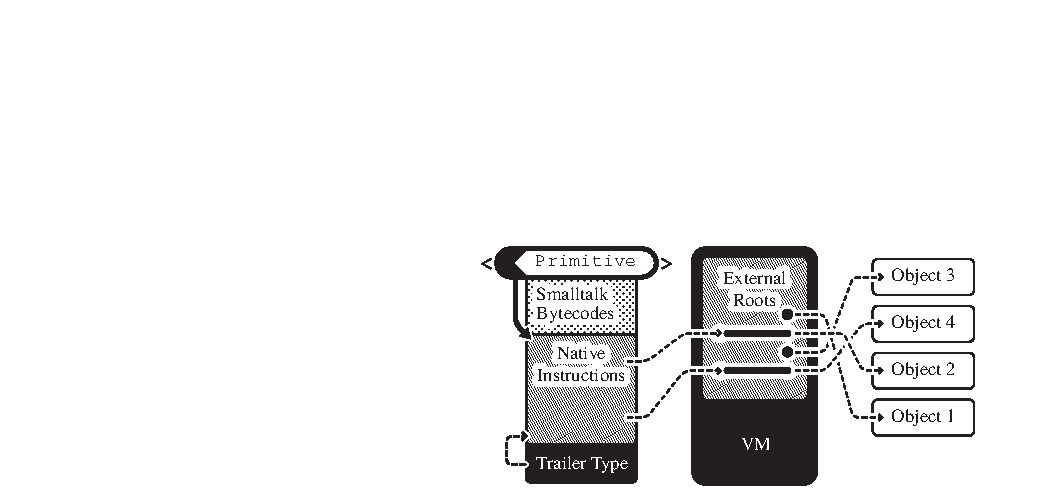
\includegraphics[scale=\imagescale]{externalRoots}
	\caption[Benzo External Roots]{Pointers to objects registered as external roots are pinpointed at fixed offset in global \VM-level object.
	\sm{You can argue differently here, GC depends on VM, (you are doing stuff that is supposed to be applicable in wider context) so, you are looking for a more general solution, one that doesn't put constraints on the type of GC... Voila, your laziness becomes something positive)}}
	\figlabel{benzo-externalRoots}
\end{figure}

\noindent \B accesses language-side objects through an indirection.
For indirectly accessing objects the \PH \VM already features a special structure, named \emph{external roots}.
This array has a fixed-location in memory which can be used to access moving language-side objects.
The \GC updates the addresses in this \VM structure after each run.
Hence we have the static address of the external roots object as an entry point to statically access \PH objects.
Summarizing, for accessing \PH objects within native code we first register it as an external root object and access it only indirectly.
This means that for native code, instead of a method-local literal array we share a global literal array as shown in \figref{benzo-externalRoots}. 
\B only adds an \ttt{Array} to the external root objects which is managed from language-side and administers all references.
\sm{Close to classic object table}

%----------------------------------------------------------------------------
\paragraph{\JIT Interaction}
\seclabel{benzo-jit-interaction}

When the \PH \VM starts the execution of dynamic generated code the execution environment changes slightly.
Similarly, when entering primitives or plugin code, the managed execution mode is left and a normal C-level execution environment is reestablished until the primitive finishes and the \VM jumps back to the jitted code.
These context switches impose an overhead and can be avoided in the case of calling native code.
For this reason we extend the \VM to support inlining of native code in the \JIT phase following the same strategy as other existing primitives which are inlined at \JIT-level.
%
\begin{figure}[ht]
	\centering
	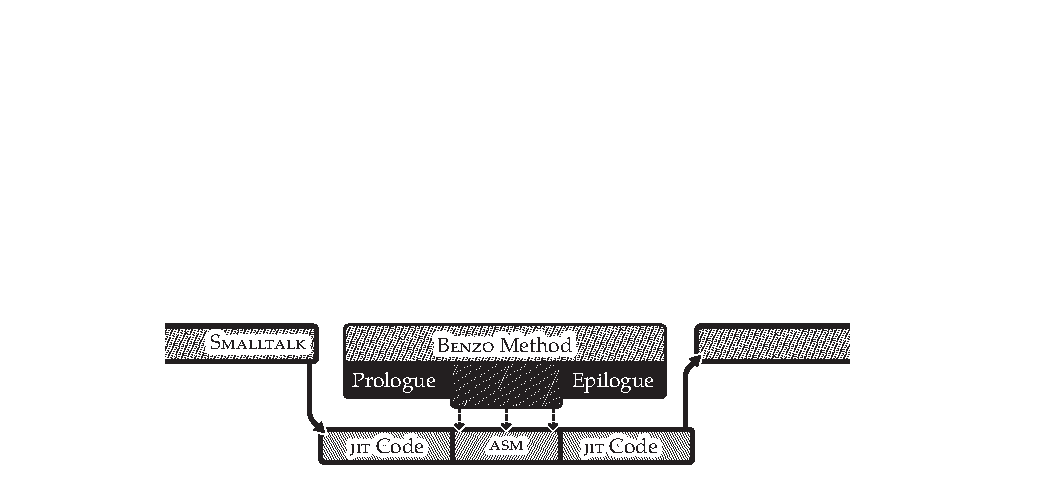
\includegraphics[scale=\imagescale]{nabujitoInline}
	\caption[\B \JIT Interaction]{\B inlining language-side native code into jitted mode.}
	\figlabel{benzo-nabujitoInline}
\end{figure}
%
\figref{benzo-nabujitoInline} shows how the native code from a \B enabled method is inlined into the \JIT infrastructure.
The \B prologue and epilogue used for managing the low-level stack are replaced by an adapted version for the \JIT.
The performance boost of this optimization is further discussed in \secref{benzo-issues-performance}.
\sm{Motivation first, why are you talking about this? Classic primitives have overhead, and you provide solution? Might not be novel,but in the context of your thesis goals it is necessary to achieve acceptable performance}


%----------------------------------------------------------------------------
\paragraph{Error Handling}
\seclabel{benzo-error-handling}

\B provides an error handling facility that allows one to return high-level error messages from the low-level code.
The native code builder provides a helper method called \ttt{failWithMessage:} that generates the proper assembler instructions to return a full error message. The following code shows an example application of this behavior.
\sm{Should you discuss the design of the native code builder? Is there anything relevant in there? I would expect it to be nicely designed to fit with your goals?}
%
\begin{stcode}[emph={asm}]{5}
failWithErrorMessage
	<primitive: 'primitiveNativeCall' 
	 module: 'Benzo' >
	 Benzo x86 generate: [ :asm :helper |
		helper failWithMessage: 'Value is not 0'.].
\end{stcode}
%
Under the hood, \B reuses the existing built-in error mechanism of \PH primitives.
However, primitives only allow for error number to be returned which limits the expressiveness of the error messages.
To circumvent this limitation \B assigns a unique error number for each error message pass to \ttt{failWithMessage:}.
\sm{It isn't a proper object that can be returned?
Shouldn't it be one in a nice clean design?}
The mapping between the two error message representation, its error number and the message string itself, happens at language-side.
\B simply reuses the existing infrastructure to improve the debugging tasks and promote a better interaction with developers.

%----------------------------------------------------------------------------
\subsection{\B's Language-Side Implementation}
\seclabel{benzo-language-side}
%----------------------------------------------------------------------------
As a key design decision, we determine to keep the interface to the low-level world minimal.
\sm{Goal!}
The following describes the features of \B at the high-level language-side.

%----------------------------------------------------------------------------
\paragraph{Code Generation}
\seclabel{benzo-code-generation}

\B delegates native code generation to a full assembler written in \PH. The following example shows how to use the assembler to generate the native code for moving \ttt{1} into the 32-bit register \ttt{EAX}.
%
\begin{stcode}{4}
Benzo x86 generate: [ :asm |
	asm mov: 1 asUImm to: asm EAX ].
\end{stcode}
%
The implementation first creates a slightly more abstract intermediate format.
The abstract operations can be extended by custom operations that may expand to several native instructions. 
\sm{Bottom up vs. top down discussion, in a thesis, I would expect top down,derived from goals and problems, I.e. By design, instead of an incidental solution that came to being without taking the overall goal into account. You need to tell me what you learned, not how you learned it/how you got to your solution}
The full features of the high-level environment are available when generating native code.
Hence complex instruction sequences can easily be delegated to other objects.
In the following example we use a \VM helper to instantiate an array. It is worth noting that all are standard message sends:
%
\begin{stcode}{5}
Benzo x86 generate: [ :asm :helper | | register |
	register := helper classArray.
	register := helper 
		instantiateClass: register
		indexableSize: 10
	asm mov: register to: asm resultRegister ].
\end{stcode}
%
\sm{Is that really high level? One thing here that's debatable is the API design, seems rather procedural. Instead of object oriented, the other thing, is is that really reflective or meta circular? How many places encode how an array is represented? The VM? Your library? Other things?

Superficially, it is just a code generation library that has nothing to do with the language it is implemented in, is that relevant? Do you need to defend such criticism? Or is that outside of the scope of your thesis?

That's why you need to get the problem statement very precise}
The \VM helper exposes a basic, low-level interface to access objects and its properties.
Additional methods cover the access to the external roots described in \secref{benzo-gc-interaction}.
In this case the \ttt{\#instantiateClass:\-in\-dex\-able\-Size:} will generate the proper native code to call to a \VM function and make sure that the side-effects of a possible \GC run are handled properly.
By default the value in the result register is returned back to the language-side. On \textsc{x86} this defaults to \ttt{EAX}.
In \secref{benzo-usecase} we introduce more substantial applications based on \B.

%----------------------------------------------------------------------------
\paragraph{Code Activation}
\seclabel{benzo-code-activation}
 
So far we only broadly described how \B activates the native code.
In a nutshell, we generate native code using our own language-side assembler and then we attach the native instructions to compiled methods as shown in figure \figref{nativeCodeMethodDetail}.
Additionally we mark the method to use a primitive defined \B plugin.
The \B primitive is responsible for the native code activation which consists of three main steps:
%
\begin{enumerate}[noitemsep]
	\item Check if there is native code in the actual compiled method and if it is compatible with the current platform.
	\item Generate native code if necessary.
	\item Activate the native code for execution.
\end{enumerate}

\noindent The first time a method with \B-based native code is activated the linked \B primitive will fail and run the normal \PH code in this method (see \secref{benzo-vm-interaction}).
This is where the actual native code generation happens.
As shown in previous examples, the native code is expressed in standard \PH code using our language-side assembler.
Once the whole code is generated, it is appended to the compiled method body leaving the existing \PH bytecodes intact.
Behind the scenes \B adds some more information to the code as the previously mentioned platform marker. 
After the native code is installed in the compiled method, we still run \PH code to restart the same \B-enabled method again.
%
\begin{figure}[ht]
	\centering
	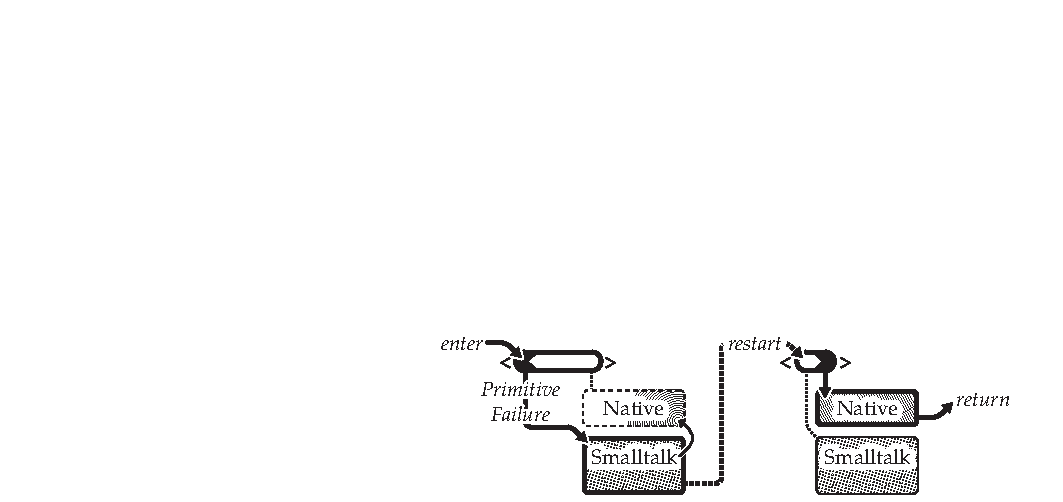
\includegraphics[scale=\imagescale]{nativeCodeActivation}
	\caption[\B Native Code Acivation]{Native code activation with \B: The first call triggers the code generation. Then the method is restarted and the native code executed.}
	\figlabel{benzo-nativeCodeActivation}
\end{figure}
%
For clarification we visualize the code activation process in \figref{benzo-nativeCodeActivation} and the following list describes the separates steps in more detail:
%
\begin{description}
\item[Activation:] In the first step (cf. \ding{182}) the \B primitive is activated.
	The primitive checks if the compiled method actually contains native code.
\item[Code Generation:] On the first activation there is no native code available yet.
	Hence the primitive will fail and the \PH body (cf. \ding{183}) of the \B-enabled method gets evaluated.
	This is where we use the \B \API and write native instructions as shown in previous examples.
\item[Code Installation:] After installing the native code in the method trailer, the \B-enabled method is reactivated with the original arguments (cf. \ding{184}).
	For activation \B uses \PH's  \ttt{\#perform:withArguments:} to reflectively restart the method.
\item[Method Reactivation:] Again we end up in the \B activation primitive (cf. \ding{185}).
	However, this time native code is present and thus the \B jumps to native code attached to the compiled method (cf. \ding{186} and returns the generated result.
\end{description}


% ===========================================================================
\section{\B in Practice}
\seclabel{benzo-usecase}
% ===========================================================================
In this section we present the outline 3 distinct solutions built on top of \B: A \FFI, dynamic primitives and a \JIT (\chapref{ffi} and \chapref{validation} provide more detailed insight).
Typically these implementations would require a custom-tailored \VM or specialized plugins.
However, we show that it is possible to implement them using the generic functionality provided by \B.

The chosen applications, starting with the \FFI, are increasingly more \VM bound.
Whereas the typical \FFI implementation is based on an separate plugin, dynamic primitives or a \JIT require persistent changes in the underlying \VM.


%----------------------------------------------------------------------------
\subsection{\NB: \B-based Foreign Function Interface}
\seclabel{benzo-ffi}
%----------------------------------------------------------------------------

\begin{figure}[h]
	\centering
	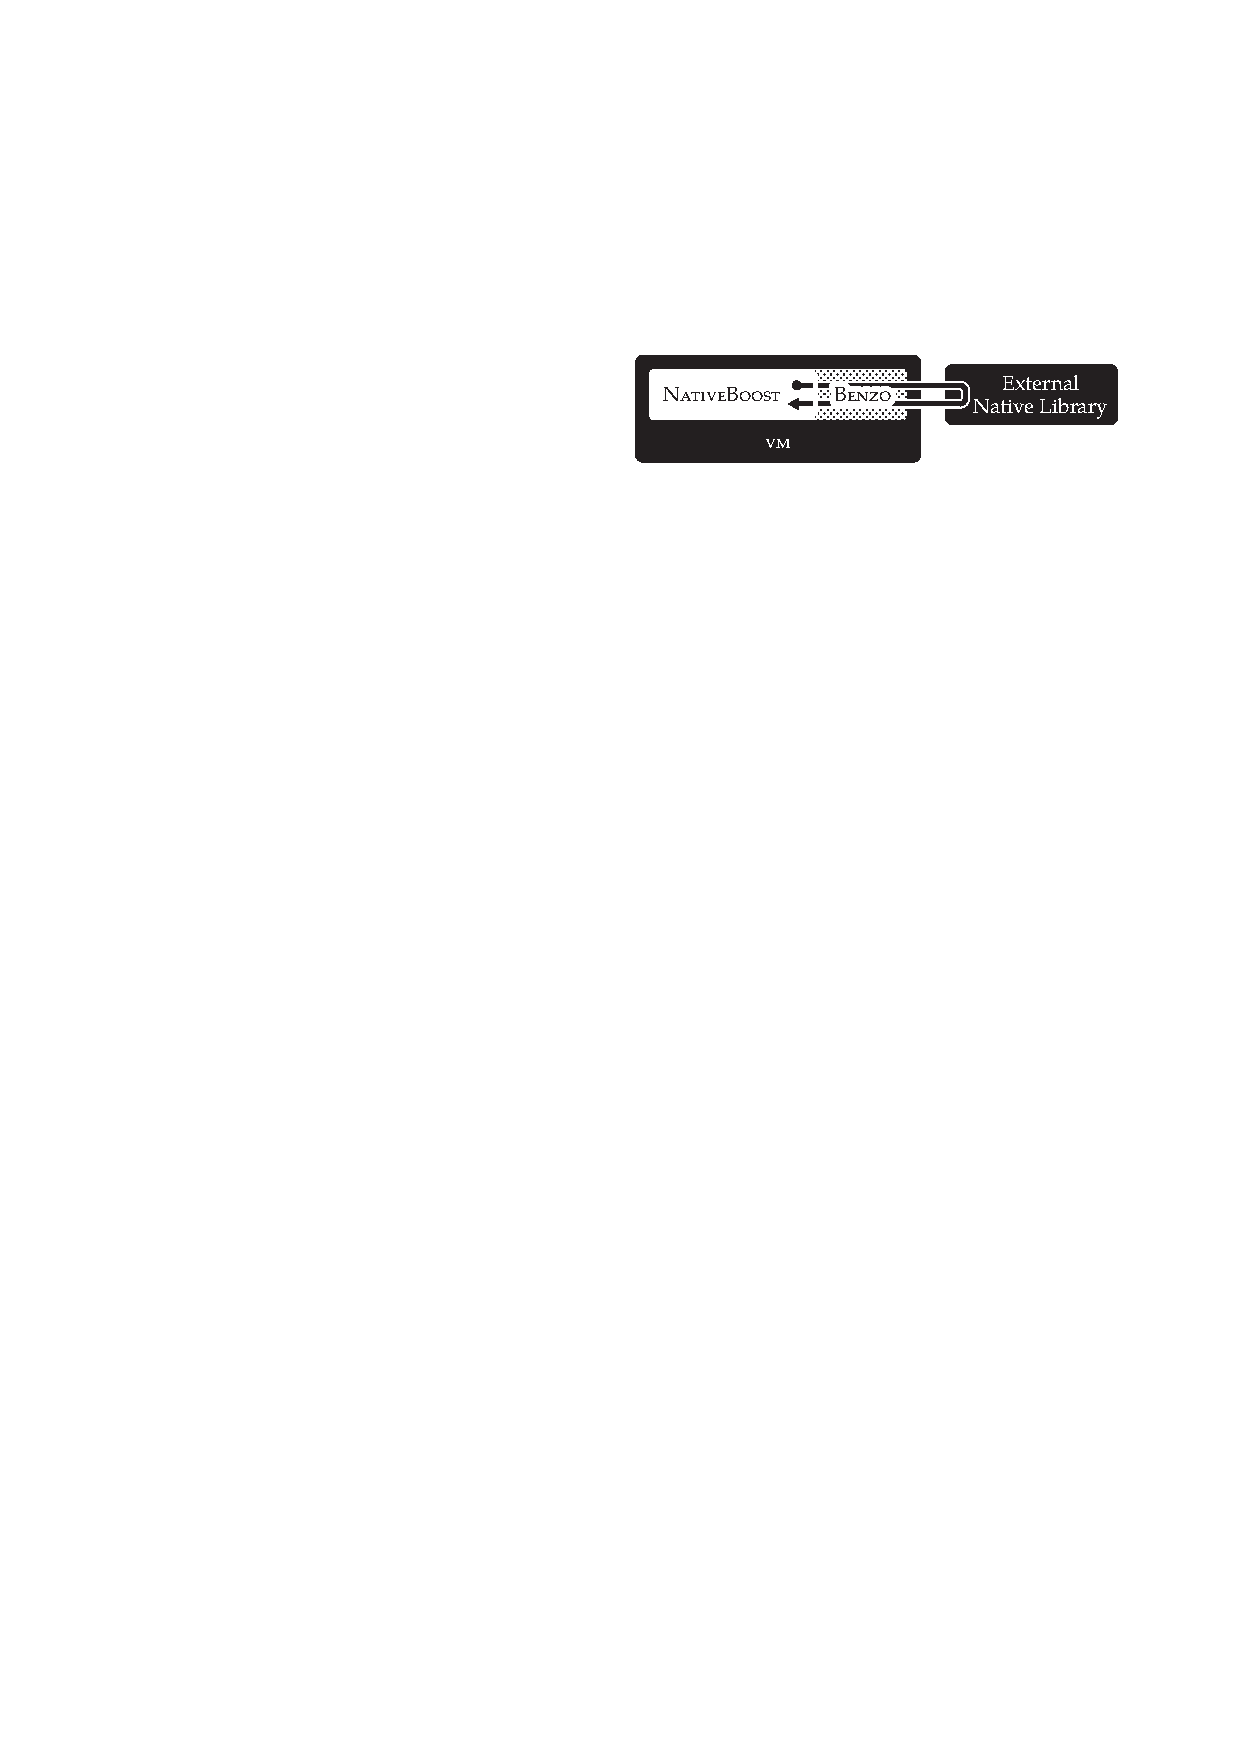
\includegraphics[scale=\imagescale]{nativeboost-overview}
	\caption[\NB Overview]{\NB generates native code at language-side with \B to perform an \FFI callout to an external function.}
	\figlabel{benzo-ffi-overview}
\end{figure}

\noindent \FFIs enable a programmer to call external functions without the need to implement additional \VM extensions.
\NB \cite{Brun13a} is a production-ready \FFI for \PH, developed on top of \B. 
For a detailed discussion of the implementation of \NB see \chapref{ffi}.
An \FFI implementation consists of two main parts: calling external functions and converting data between the two environments.
Typically a big percentage of these two parts are implemented at \VM-level with statically defined bindings.
Relying on \B's capability to dynamically generate and execute native code we developed a complete \FFI at language-side.
This way the \VM no longer requires to have a specific \FFI extension.

A very simple example to illustrate the functionality of \NB is to access the current environment variables with the \ttt{getenv} C function.
\ttt{getenv} takes a name as single argument and returns the value of that environment variable as a string:
%
\begin{stcode}{4}
getenv: name
    ^ NativeBoost call: 'String getenv(String name)'
\end{stcode}
%
In this example \NB automatically detects, using reflection, that the argument for the \PH method corresponds to the one of the low-level C function.
The most important aspect about this example is that it is written with standard \PH code, a property that extends to almost the complete implementation.
\NB, additionally to the native code activation, relies on two simple primitives provided by \B to retrieve addresses of external functions (\ttt{dlsym}) and to load external libraries (\ttt{dlopen}).

\NB generates the glue code to call external functions dynamically at run time.
It relies on \B's features presented in \secref{benzo-language-side} to generate and activate native code at runtime.
This gives \NB a significant advantage over static approaches: the generated native code is specific to the callout.
For instance in the \ttt{getenv} example, the marshalling code for converting from the internal \PH strings to C strings is written a small assembler routine.
In this specific context, the assembler code is faster than any language-side code.
Yet \NB is very flexible since all these conversion routines are defined at language-side. 
Each language-side library can define its own highly efficient conversion routines for types that are used in \FFI callouts, which is not directly possible to do with a \VM extension.


%----------------------------------------------------------------------------
\subsection{Reflective Primitives}
\seclabel{benzo-waterfall}
%----------------------------------------------------------------------------

\begin{figure}[h]
	\centering
	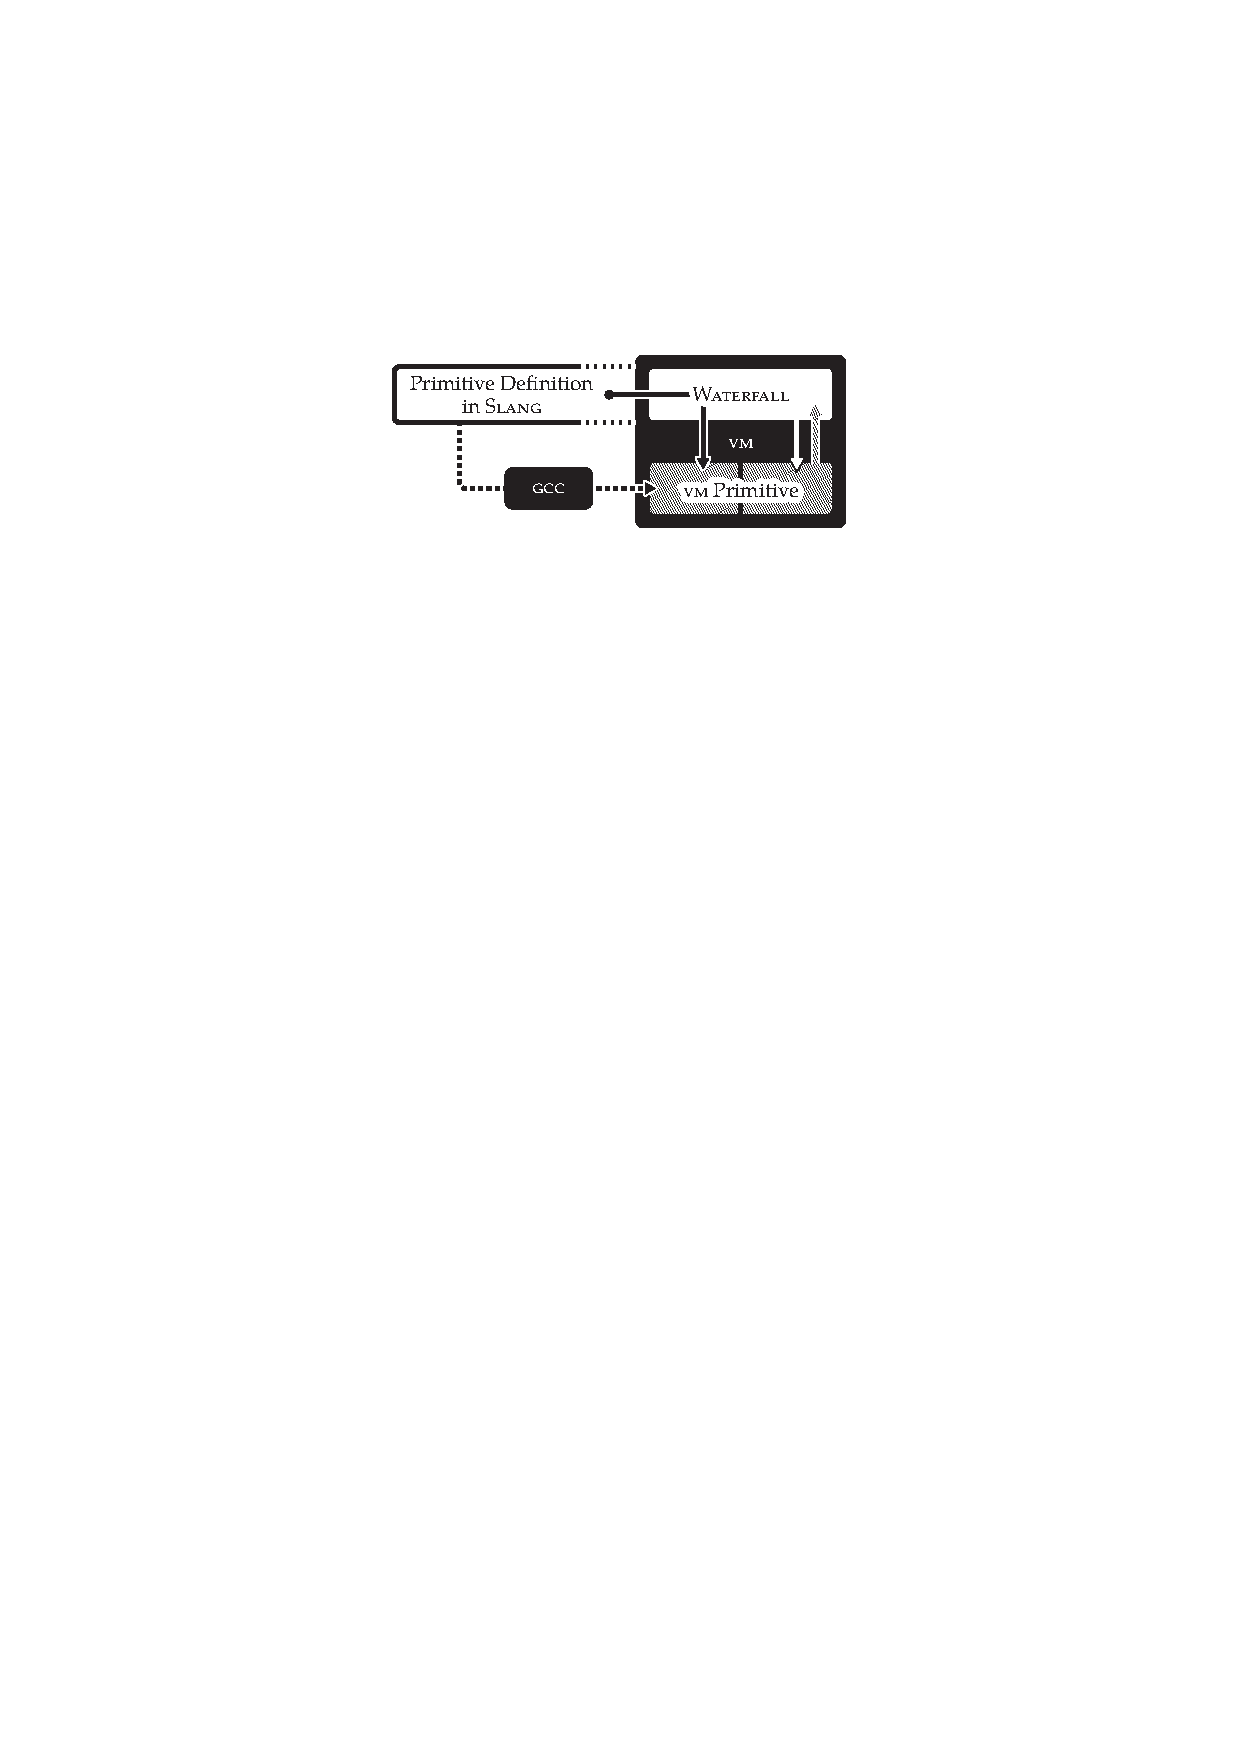
\includegraphics[scale=\imagescale]{waterfall-overview}
	\caption[\WF Overview]{\WF reuses the definitions of \VM primtives written in \Slang and compiles them dynamically. The same primitive definition is used for generating the static primitive at \VM compilation time.}
	\figlabel{benzo-waterfall-overview}
\end{figure}

\todo{by Guido Chari}
\noindent The second \B-based application we present takes the concept of our \FFI solution further.
\sm{Don't imply! Be explicit! The second is something... You neither name it nor give me clues what you are going to talk about.

And also, start out with telling my what waterfall is concretely, you are now telling me what it ain't, by telling me what native boost doesn't do. That can come later, first, I want to know why I should read this section}
\NB allows us to call external functions by generating the callout code at language-side.
From an abstract point of view we replace language-side methods with native routines.
\NB does not directly synthesize new features but only makes external functionality available to the language itself.

As explained previously in \secref{benzo-vm-interaction} \B uses \PH's primitives to activate native code.
Since \PH is an open system we can extend this behavior to existing methods.
Instead of simply adding new methods which call native code we present \WF, a solution that modifies existing primitive methods and replaces them with \B-based native code.
Instead of manually generating the sources for the primitives we reuse existing code.
The \VM used for \PH is metacircular, the \VM sources are written in the same language, in our case in a simplified subset of \PH called \Slang.
Hence, the complete definition of the \VM including the primitives can be made accessible at language-side by loading the \VM sources.
\WF then takes the primitive definition written in \Slang and compiles it to native-code.

As \figref{benzo-waterfall-overview} illustrates, \WF extends the lifetime of the metacircular \VM definition to the actual language runtime.
\sm{Why does this paragraph sound like it is going to talk about something very different? I first want to know how the compilation is done, do you have a slang interpreter or something?}
By default the primitive definitions written in \Slang are only used to generate the \VM source in an intermediate step.
A C-compiler such as \GCC generates the final binary.
By doing so the high-level primitive definitions are absorbed by the intermediate compiler infrastructure.
The final binary has no reflective capabilities anymore.
From within \PH we can only activate primitives but the abstract definition is no longer accessible.
Hence, we can not directly modify primitives directly without the original \VM sources loaded.
\sm{Are you sure you are fixing this, I.e., that the original code doesn't have to be present? Are you de compiling native code?

And, I still don't know how waterfall does the compilation, does it also use the c compiler?}

\WF provides a complete metacircular infrastructure for primitives.
\sm{Bla Bla, that doesn't tell me anything, because I don't know what that means in this context}
We use \WF to modify primitives on the fly.
For instance it becomes possible to instrument the crucial \ttt{basicNew} primitive, something that is almost impossible to achieve with pure language-side reflection.
\sm{I intercepted basicNew on the language side in my OMOP, no VM support necessary! I think you want to say something different.

(I did not change allocation, but I set the owner of each object by 'wrapping around' basicNew and basicNew:) }
Since this primitive is used for object creation, each attempt to monitor this primitive is doomed.
If the monitoring code itself would create a new object, infinite recursion would be inevitable.
\sm{True, but what's your point? Your solution ain't solving that either}
In \secref{val-waterfall} we explain in more detail the difficulty of such a task along with promising performance evaluations.



%----------------------------------------------------------------------------
\subsection{\NBJ \JIT Compiler Prototype Outline}
\seclabel{benzo-nabujito}
%----------------------------------------------------------------------------
\todo{Adapt to the findings of \NBJ that it is currently not possible to implement on top of the \VM}
In this section we present \NBJ, a \B-based approach for a language-side \JIT compiler.
\NBJ goes even further than \WF using almost the same techniques.
\sm{I still have not even an intuition what waterfall does :(}
However, instead of focusing on primitives, \NBJ generates native executable code for standard \PH methods.
Primitives tend to be more low-level, whereas \NBJ focuses on high-level \PH code. 

\begin{figure}[h]
	\centering
	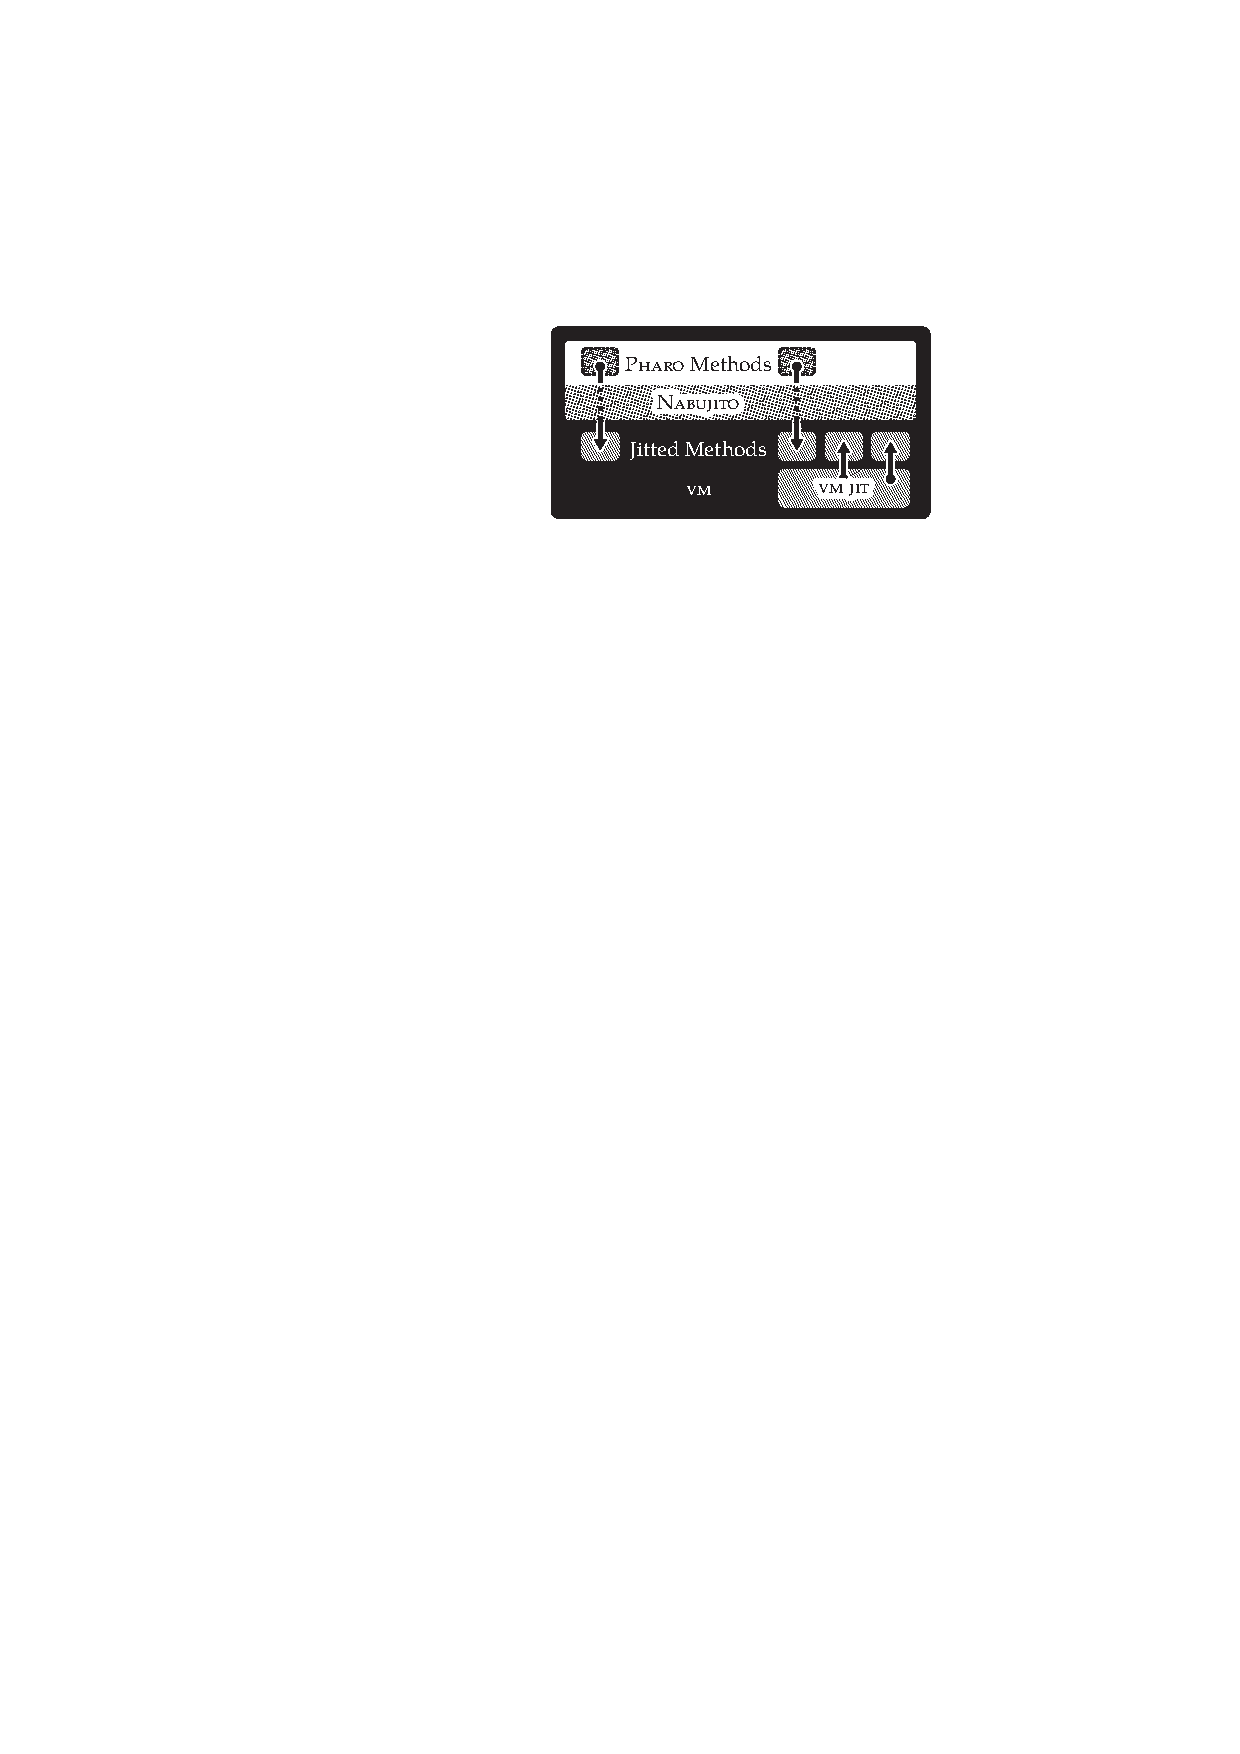
\includegraphics[scale=\imagescale]{nabujito-overview}
	\caption[\NBJ Overview]{\NBJ compiles standard \PH methods with the help of \B to the same format the \VM \JIT uses.}
	\figlabel{benzo-nabujito-overview}
\end{figure}

\noindent The \PH \VM (originally \urlfootnote{\textsc{Cog vm}}{http://www.mirandabanda.org/cog/}) already comes with a \JIT that translates bytecodes to native instructions.
It transforms \PH methods into slightly optimized native code at runtime.
The most complex logic of the \JIT infrastructure deals with the dynamic nature of the \PH environment.
Methods and classes can be changed at runtime and that has to be addressed by the \JIT infrastructure.
This implies that an efficient \JIT infrastructure needs substantial access to language-side structures; in our case classes, methods.
\sm{Really? I don't believe that. That only means you need to be able to invalidate code, something that ever speculative \JIT does, and you said before that there aren't any VMs fulfilling your criteria. So, be more precise here, this is too sloppy and too broad of a statement}
This information is readily accessible in \PH through the standard reflective \API.
However, at \VM-level this requires more effort, and thus imposes strong requirements on the design of classes and methods at language-side.
The \JIT infrastructure is a hybrid between \VM logic and language-side reflection.

The \JIT compiler, by which we refer in this context to the transformation of bytecodes to native code, represents a small part of the whole \JIT infrastructure.
There exists more important stages \sm{Reference unclear, what is more important than what?} as an additional register allocation pass to reduce the number of stack operations \cite{Mira99a,Mira11a}.
The existing \JIT infrastructure is implemented in \Slang \cite[Ch.\ 5]{Blac09a} as the rest of the \VM.
We believe that a hard-coded static and low-level implementation is not optimal for several reasons:

\begin{itemize}
	\item Optimizing \PH code requires strong interactions with the dynamic environment.
	\sm{Why? Java proves you wrong by your own criteria, I believe, as does Self most probably}
	
	\item Accessing language-side properties from the \VM-side is hard.
	\sm{Hard? Or impossible? And why is that? Just because the interface isn't well defined?
	This criterion is not useful as it is phrased now}
	
	\item Changing the \JIT compiler requires changes at \VM-level.
	\sm{So what? You are implying here assumptions about development approach, stuff you discussed earlier, I think. So, changing the VM takes a lot of effort, which you outlined earlier? That's your point? You want that to be possible much more interactively? Then say that, instead of broad phrases}
	
	\item The \JIT reimplements primitives for optimization reasons resulting in code duplication.
	\sm{This problem is now noted down on the list of things your reviewers are expecting you to solve, I hope you do...}
\end{itemize}

\paragraph{Implementing \NBJ with \B}
Motivated by the aforementioned implications of a \VM-level \JIT we conceived \NBJ a prototype \JIT compiler based on \B.
\NBJ is an experimental \JIT implementation which replaces the bytecode to native code translation of the existing \JIT infrastructure with a dynamic language-side implementation.
\NBJ is implemented as a visitor over the existing intermediate bytecode representation. 
Additionally we reimplemented \sm{Oh oh, didn't you say reimplementing stuff is evil? Perhaps make this more clear, and avoid the word, you just put on the list of things you want to solve...} vital native routines for the \JIT which are not directly exported by the \VM using \B. 
\NBJ relies on the following \VM-level infrastructure to manage and run native code for any \PH method:

\begin{itemize}[noitemsep]
	\item Fixed native code memory segments.
	\item Routines for switching execution contexts.
	\item Native stack management.
\end{itemize}

\paragraph{Dynamic Code Generation}
For standard methods \Nabujito takes the bytecodes and transforms them to native code.
It also applies optimizations such as creating low-level branches for \PH level branching operations like \ttt{if\-True:}.
Optimizations for additional methods are all implemented flexibly at language-side.
Wherever possible, we reimplement the same behavior as the existing native \JIT compiler.
Eventually the native code is ready and \B attaches it to the existing compiled method.
When the language-side jitted code is activated \B ensures that we do not have to leave the \JIT execution mode, and thus we can call methods at the same speed as the existing \JIT.
\secref{val-nabujito} gives a more detailed insight of the design and performance of \NBJ.



%============================================================================
\section{Performance}
\seclabel{benzo-issues-performance}
\seclabel{benzo-performance}
%============================================================================

In this section we discuss the general performance characteristics of \B for the three example applications outlined in the previous section.
A more detailed validation is presented later in \secref{ffi-performance} (\FFI), \secref{val-waterfall-performance} (\WF) and \secref{val-nabujito-performance} respectively.

\paragraph{One-time Code Generation Overhead} 
\B allows the generation of specialized and thus efficient native code.
In \secref{benzo-benzo} we explained how \B causes only a one-time overhead for native code generation. 
Thereafter it is cached for later activations.
The three use case presented in \secref{benzo-usecase} heavily benefit from this fact.
Generating code at language-side poses a significant overhead compared to invoking a precompiled native implementation.
However, this is only a one time overhead.
For instance the \B-based \FFI implementation presented in \secref{benzo-ffi} outperforms a \VM-level \FFI-plugin due to a more flexible language-side implementation which generates specialized code for each \FFI callout. 
These results are shown in the following \tabref{benzo-ffi-performance-simple}.

% ---------------------------------------------------------------------------
\subsection{\B-based \FFI}
\seclabel{benzo-nb-performance}
% ---------------------------------------------------------------------------

The first mini performance evaluation we present is for \NB the \B-based \FFI.
Compared to a static plugin-based \FFI implementation \NB has only a one-time startup overhead.
Generating the native code at language-side is substantially slower than directly setting up all the conversions and calling the external functions from C code. 
In certain cases the penalty for the language-side code generation of \NB is as high as a factor of 100 compared to classic approaches.
\sm{Approaches, to what do you compare exactly? Be more precise with those comparisons, you are slower than what exactly? Otherwise, I stop reading, because you are just saying the your whole approach is doomed...}
Under the assumption that the method is called several times this overhead may be considered negligible.
An in-depth evaluation of \NB comparing against other solutions is presented later in \chapref{ffi}.
The following table contains a performance comparison of three different \FFI implementations for \PH that represents the typical showcase.
\sm{Use case, not show case, showcase is something specifically selected that shines, nothing typical about that}

\begin{table}[!ht]
    \centering
    \begin{tabular}{rSS}
                   					& {Call Time [ms]} & {Relative Time} \\\midrule
        \NB         				& 10.53(35)        &        1.0 \\
        \Alien, language-side \FFI  & 31.09(94)        & \approx3.0 \\
        C-\FFI, plugin-based \FFI   &  9.55(64)        & \approx0.9
    \end{tabular}
    \caption[Basic \B-based \FFI Performance]{Different \FFI implementations in \PH evaluating \ttt{abs(int)}. \Alien does marshalling at language-side while \FFI does everything in \VM plugin written in C.}
    \tablabel{benzo-ffi-performance-simple}
\end{table}

\noindent \tabref{benzo-ffi-performance-simple} measures the accumulative time of 100'000 \FFI calls.
Included in these numbers is at least one additional \PH message send to activate the \NB method containing the actual call to the C function.
\NB outperforms the existing language-side \FFI (\Alien) and the implementation (C-\FFI).

The existing language-side \FFI has a generic plugin to call C-functions and performs type-conversions at language-side.
However, converting \PH objects from and into low-level data is comparably expensive.
In \NB this happens directly in custom generated native code and is thus significantly faster.
The plugin-based \FFI is also slower than \NB since it still has generic conversion function for \PH objects, albeit written in C and thus faster than in \Alien.
However, \NB custom tailored \ASM code is still faster than the hard-coded C counterpart.
\sm{There something wrong with either the number so the text, the CFFI is faster according to call time}

This simple \FFI evaluation already highlights the core benefit of \B to generate very customized native code when needed.
Yet we have to emphasize that \NB is based on the \B infrastructure whereas the other solutions require both a \VM plugin whose sole purpose is to enable the \FFI functionality.
Furthermore \NB benefits from the \JIT interaction described in \secref{benzo-jit-interaction}.
This optimization is especially an important optimization factor when calling out small helper routines where the context switch from jitted mode is no longer negligible.

% ---------------------------------------------------------------------------
\subsection{\B-based Dynamic Primitives}
\seclabel{benzo-wf-performance}
% ---------------------------------------------------------------------------

As the second performance evaluation of \B we present a simple use case of dynamically implementing a primitive with \WF.
For comparing performance we implement a very simple integer operation primitive (\ttt{$>$}) using three different approaches.
The first approach is the implementation with \WF.
The second is to run the language-side implementation that is triggered whenever the standard primitive failed.
Finally the fast standard primitive provided by the \VM.
We run the three approaches by measuring the cumulative time over one million primitive activations averaged over 100 runs.
The absolute numbers are less important than the relative factor between them.
We present the results of this experiment in \tabref{benzo-waterfall-performance}.
%
\begin{table}[!ht]
    \centering
    \begin{tabular}{rSS}
		Primitive Type  & {Running Time [ms]} & {Relative Time} \\\midrule
		\VM			    &   6.40(14)          &         1.0 \\
		\WF             &  22.80(17)          & \approx 3.6 \\
        Reflective	    & 195.00(16)          & \approx30.0
    \end{tabular}
    \caption[Basic \B-based Dynamic Primitive Performance]{Comparing running time of different implementations of integer arithmetic primitive.
    \sm{While it might not matter for the numbers, for a clear setup it would be advisable to not include the failing of the primitive in the measurement.
    
    From the text it is not clear whether you do or don't }}
    \tablabel{benzo-waterfall-performance}
\end{table}
%
\WF clearly outperforms a purely reflective solution.
As explained in \secref{benzo-waterfall}, replacing a crucial primitive with simple language-side is not straight forward.
If the replacement code triggers the very same primitive again we are trapped in a meta-recursion loop \cite{Chib96a}.
To avoid this, the \PH code for the replacement of \ttt{$>$} checks that the current activation of the primitive is not recursive.
This comes at a substantial cost and is the main overhead factor.

\WF is a factor $3.6$ slower than the standard implementation.
First we have to state that \WF uses a very simplistic compilation strategy with many optimizations opportunities left out.
Second, the optimized \VM primitive is also reimplemented in the \JIT to avoid the overhead of switching execution context (see \secref{benzo-vm-interaction}).
\sm{I don't get the second part}

This results thus makes a whole new set of runtime extensions feasible that were previously limited by their strong performance penalty.
Furthermore the performance penalty over a completely optimized \VM solution that has extreme optimization techniques, such as inlining and register allocation, is less than a factor of $4$.
A more detailed analysis of \WF is available later in \secref{val-waterfall-performance}.
\sm{If you do detailed stuff later, I would drop this 'mini' stuff here. One evaluation is enough, this section/chapter can stand on its own and should make the ideas clear}


% ===========================================================================
\section{Related Work}
\seclabel{benzo-related}
% ===========================================================================
\sm{This chapter needs work, I don't think the structure works integrated in your thesis.

And, well, I find related work here at this place, a little strange}
In the context of \B we see a variety of related work spawning different abstraction levels.
On a more abstract scale \B allows for a new way of extending the complete language runtime, hence we classify the related work according the following categories show in \figref{benzo-extensionComparison}: general language-side extensions, extensions using reflection, \VM-level extensions, and hybrid approaches.

We present now an overview of the approaches used to extend a language runtime and expose their limits.
High-level languages are in general sustained by a \VM and a vast set of libraries written in the language itself. 
Extending or improving the existing language runtimes is a difficult task.
In most cases the \VM is considered as a black box.
Additionally the \VM is written in a completely different language using another abstraction level than the one it supports.
Typically high-level language \VMs are written in C or C++.
To address extensions in this context there exist some known approaches:
\sm{All the introduction stuff should be done in the proper chapter, 2, I guess }

\begin{description}[noitemsep]
	\item[Language-side Library] based on implementing a new or existing library. 
	\item[Reflective Extension] relying on reflective features of the language. 
	\item[\VM Extension] by writing plugins or changing the core of the \VM.
	\item[Hybrid Extension] by accessing external libraries using \FFI.  
\end{description}
%
The relation between the side concerning the abstraction and implementation levels (\VM vs. language) of these extensions is illustrated in \figref{benzo-extensionComparison}.

\begin{figure}[h]
	\centering
	\begin{subfigure}[t]{0.45\textwidth}
		\centering
		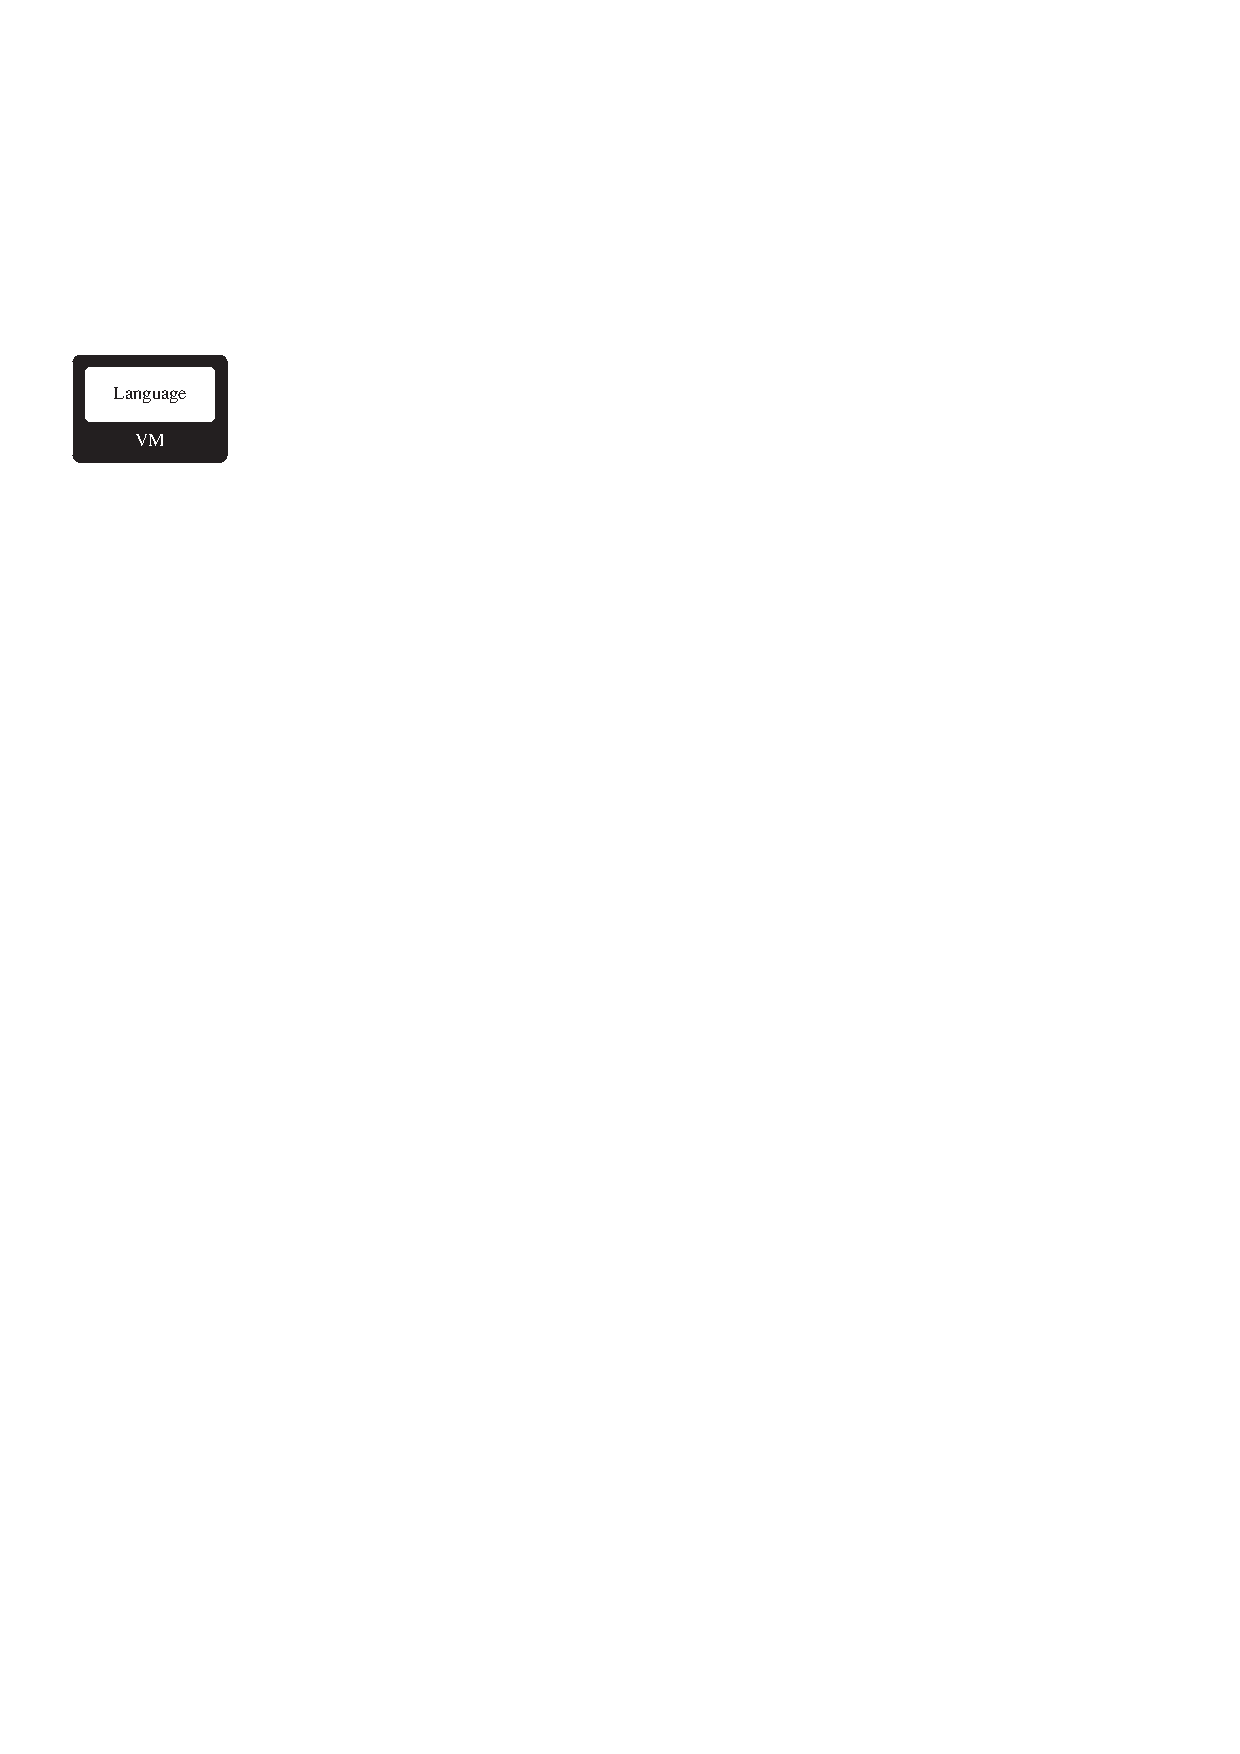
\includegraphics[scale=\imagescale]{extension-language}
		\caption{Language running on a standard, unmodified \VM.}
	\end{subfigure}\hspace{0.09\textwidth}
	\begin{subfigure}[t]{0.45\textwidth}
		\centering
		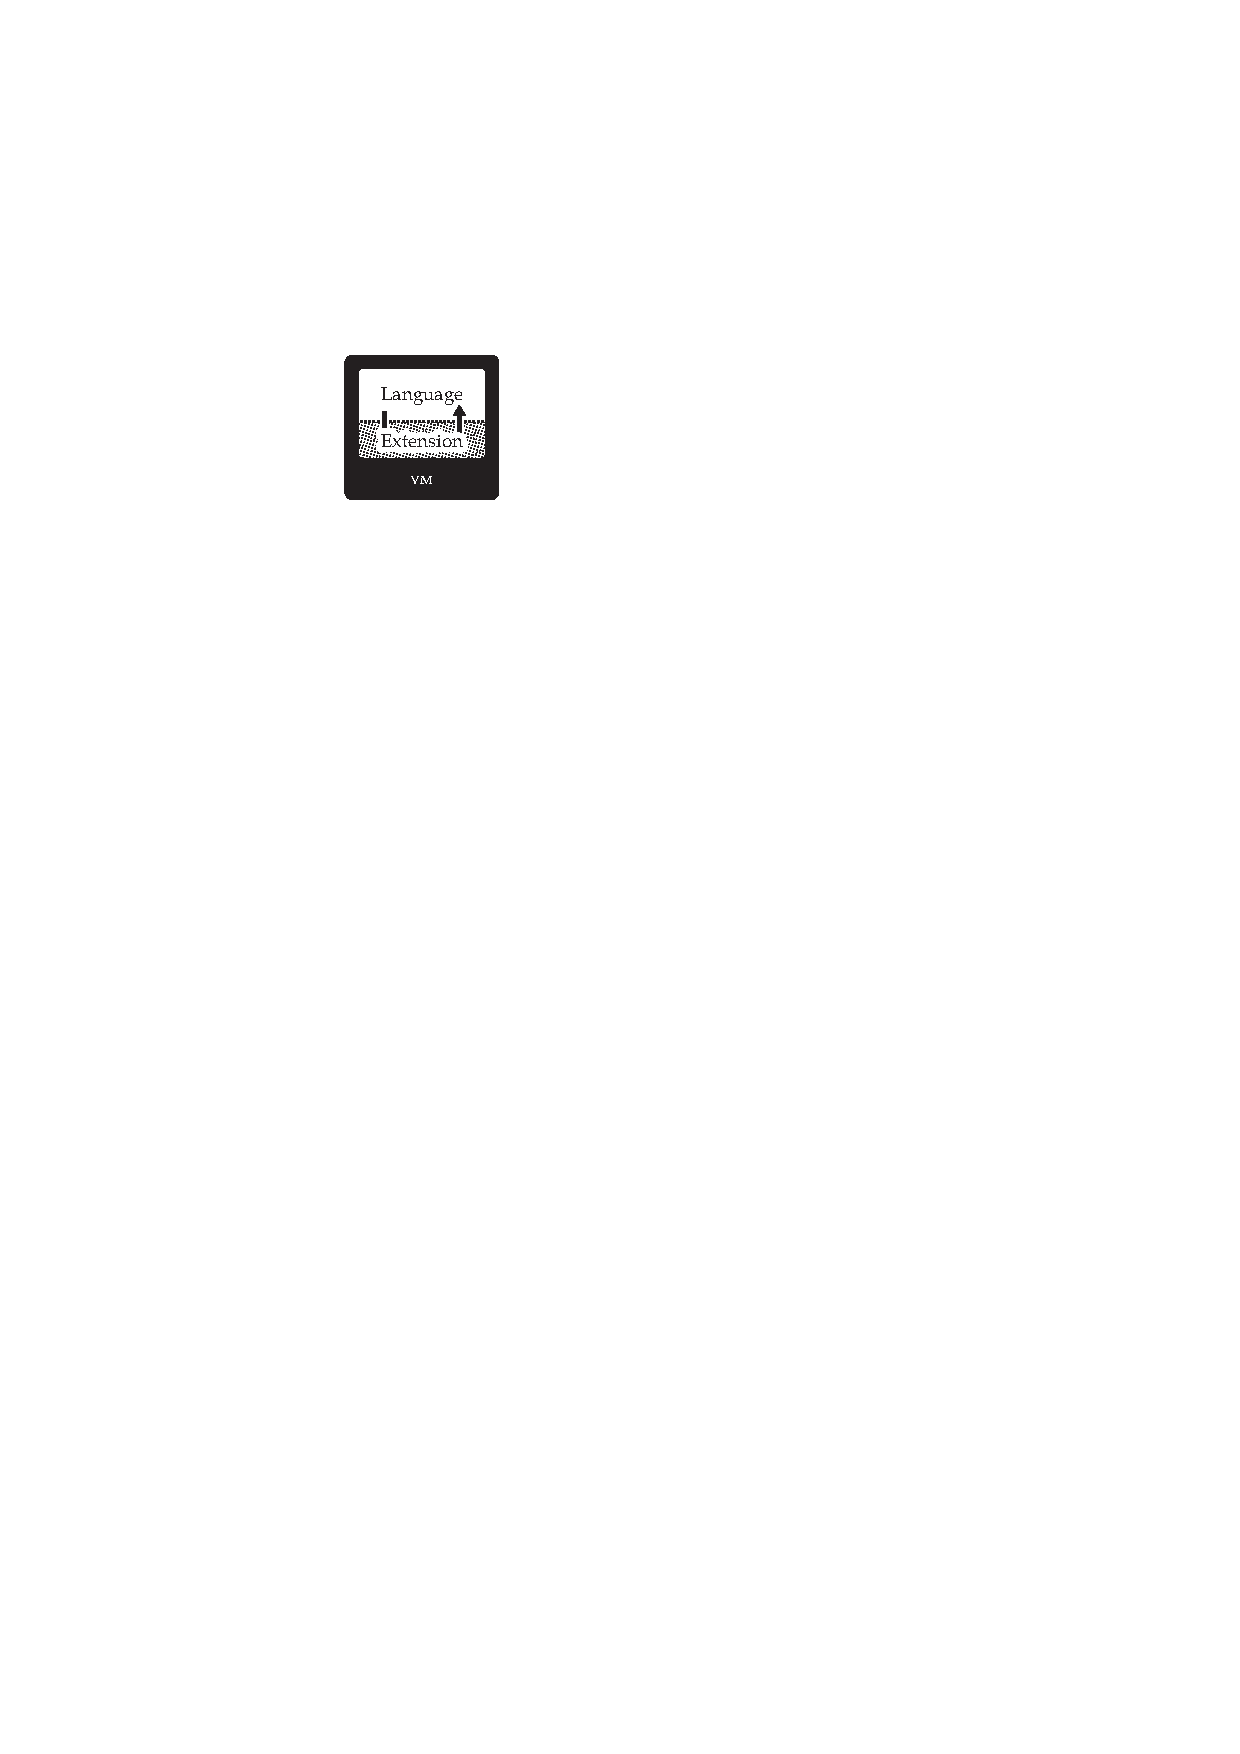
\includegraphics[scale=\imagescale]{extension-language-library}
		\caption{Language-side implementation of an extension.}
	\end{subfigure} \\
	\vspace{\baselineskip}
	\begin{subfigure}[b]{0.45\textwidth}
		\centering
		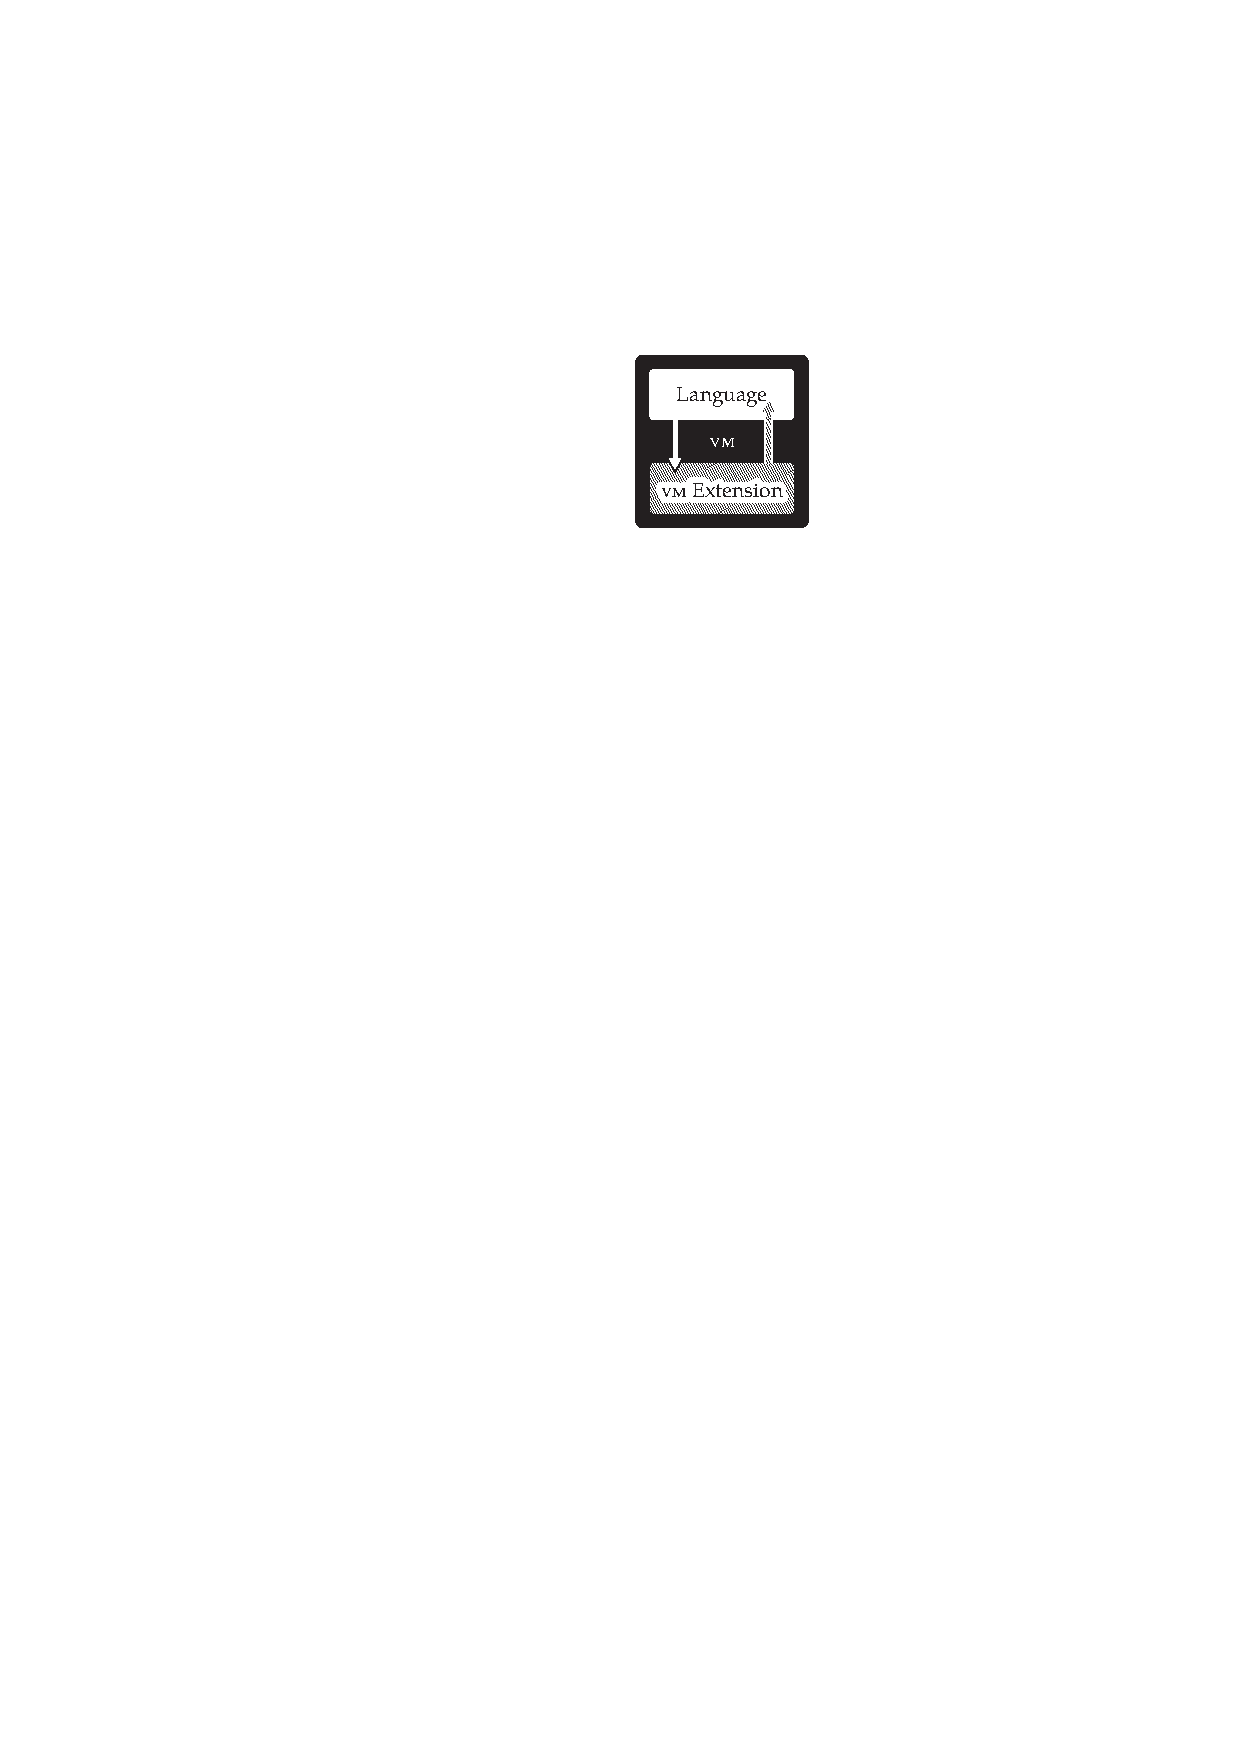
\includegraphics[scale=\imagescale]{extension-vm}
		\caption{Language using features from a \VM extension.}
	\end{subfigure}\hspace{0.09\textwidth}
	\begin{subfigure}[b]{0.45\textwidth}
		\centering
		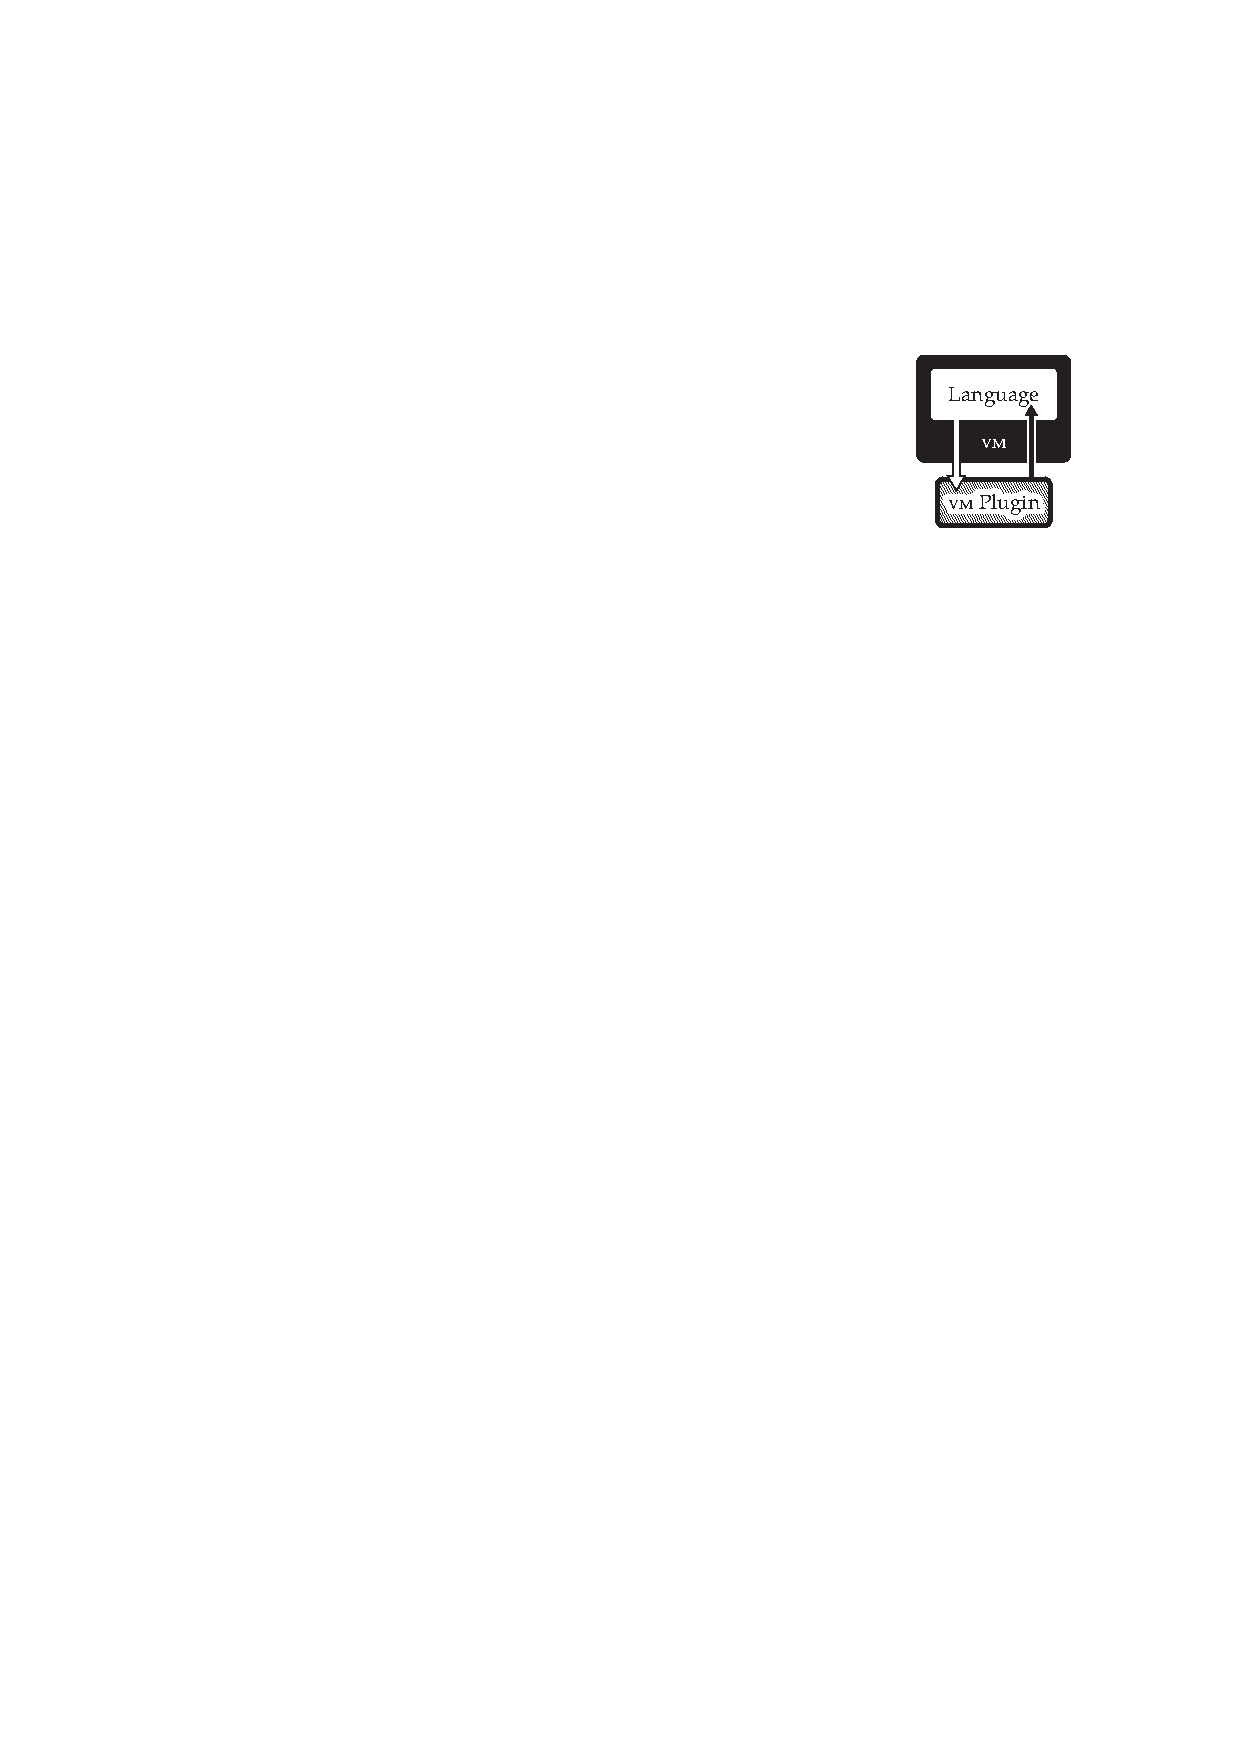
\includegraphics[scale=\imagescale]{extension-plugin}
		\caption{Language using features from a separate \VM plugin.}
	\end{subfigure}
	
	\caption[Language Extension Mechanisms]{Comparison of different extension mechanisms}
	\figlabel{benzo-extensionComparison}
\end{figure}

%----------------------------------------------------------------------------
\subsection{Language-side Library}
%----------------------------------------------------------------------------

The most straight forward solution for extending a language is to write libraries within the language itself. 
This option provides the advantage that the aggregate behavior is accessible and evolvable for any language developer.
However, language-side libraries are constrained by the underlying managed language runtime.
The \VM separates the language from the low-level internal details.
As a consequence language-side libraries are not feasible for all feature requirements.
For instance the previously mentioned example of instrumenting the language runtime is not possible as a standard language-side extension without a considerable performance loss.
So, even though we prefer extensions and optimizations at language-side, there are certain limitations of a managed language runtime that can not be circumvented.
If all language-side optimization opportunities have been exhausted it is exposing the need to resort to lower level approaches.

\begin{quote}
Language-side libraries are constrained to the capabilities of the underlying \VM and thus not general enough. 
Additionally not all performance bottlenecks can be addressed at language-side.
\end{quote}

%----------------------------------------------------------------------------
\subsection{Language-side Reflective Extensions}
%----------------------------------------------------------------------------

This is a specialization of the previous approach but in the context of reflective environments.
For instance, Meta Object Protocols (\MOP) \cite{Kicz91a} based on reflection \cite{Maes87a} are used to define certain control points in the system to change the language.
By composing meta objects it is possible to even modify the semantics of the language. 
Several languages such as \PH, \ST, \urlfootnote{\Python}{http://python.org/}, \urlfootnote{Ruby}{http://www.ruby-lang.org/}, and others provide reflective capabilities with different depths \cite{Ande98a,Van10a}.
However, most modern programming languages only have very limited support for intercession.
Hence the possibilities for dynamically changing language semantics or features are limited. 
Furthermore reflective capabilities are hard to implement efficiently.
Reflection imposes substantial performance penalties on most computations by postponing bindings \cite{Male96a}. 
Nevertheless, there are exceptions for a subset of reflective behavior which are implemented efficiently using a high-level MOP \cite{Vran12a}.
Though these approaches remain as a few exceptions.
In the typical low-level \VM it is difficult to gain reflective access to language-side objects.
Similar to the previous case, our goal is to extend language features in a general way and it was shown that this is only partially possible by reflective extensions. 

\begin{quote}
Reflective capabilities are not enough for general extensions. Even when suitable, they usually pose a significant performance overhead up to the point where they become unfeasible.
\end{quote}

%----------------------------------------------------------------------------
\subsection{\VM Extensions / Plugins}
\seclabel{benzo-vm-extensions}
%----------------------------------------------------------------------------
\sm{Yes, I think all that needs to be folded into chapter 2}
Another approach to extend add new features to a programming language is to extend the \VM.
At this level we differentiate between two extension mechanisms: \VM plugins and modified \VMs itself.
Plugins are direct bindings to external libraries described at \VM-side or libraries linked to the \VM executable \cite[Ch.\ 5]{Blac09a}. 
They provide a performance boost in comparison to pure language-side solutions.
Using highly optimized native libraries it is straightforward to outperform code written at language-side.
Typically, even very complex \VMs such as the \Self \VM \cite{Unga07a} provide a clean interface to write plugins.
Missing high-level concepts make them harder to maintain than language-side code.
Depending on the added feature the plugin interface may prove to be too inflexible and the only choice is an modified \VM.
Such a fork comes at an even higher cost of maintenance.
In the following paragraph we will explain the these two main limitations we found when working with plugins: a certain abstraction mismatch compared to host language and the limitations imposed by a clean plugin interface.


\subsubsection*{Problem: Abstraction Mismatch}
Plugins are commonly written in the same language as the \VM, at a low abstraction level.
The abstraction difference compared to a language-side extensions makes it difficult for standard programmers to modify or write \VM plugins.
Few exceptions are self-hosted languages \cite{Unga05a,Wimm13a,Rigo06a}.
To support a fluent development process, \VMs should come with an infrastructure for building extensions at same abstraction level as the provided language.
Instead \VMs tend to be rather complex which includes the whole development cycle.
For example, only a few \VMs have high-level debugging facilities \cite{Inga97a,Unga05a,Wimm13a}.
It is more common to be stuck in the compilation step waiting for the debugging binary to be ready.

\paragraph{\VM Generation Framworks}
The lack of abstraction for \VM-level extensions can is addressed by \VM generation frameworks in general.
They try to abstract away the complexity of the \VM and use high-level languages as compiler infrastructure.
A very successful research project is \urlfootnote{\textsc{Jikes} Research \VM}{http://jikesrvm.org/} (former \textsc{Jalapeño})~\cite{Alpe99a}.
It uses \Java to metacircularly define a \Java environment which then generates the final \VM.
A similar framework is \urlfootnote{\PyPy}{http://pypy.org/} \cite{Rigo06a} a \VM framework including an efficient \JIT. 
\PyPy uses a restricted subset of the  \textsc{Python} language named \textsc{RPython} which is then translated to various low-level backends such as C or \textsc{llvm} code.
There exist several different high-level language \VM implementations on top of \PyPy such as \ST \cite{Bolz08a} or \textsc{Prolog}.
However, its main focus lies on an efficient \JIT generator mainly for a \Python interpreter, and not on a direct, language-side assembler interface.
\PyPy encourages to use reflection at compile-time which helps to write a maintainable code base.

\subsubsection*{Problem: Plugin Limitations}
Once a programmer is fluent at \VM-level a clean plugin interface is a big aid in terms of maintenance.
However, certain functionality can not be added by simply creating a separate plugin that encapsulates the new feature.
Prominent examples are \JIT support, immutability or first-class handles \cite{Arna13a}.
In all these examples core pieces of the \VM have to be modified: the \VM has to be forked.
From a \VM maintenance point of view, forks have to be avoided if possible and should only be used for critical performance issues that can not be properly addressed at language-side or with plugins.

From our experience with \PH, even promising \VM experiments are not maintained for a long time.
An example for that is the modified \VM supporting back-in-time debugging implemented for an early version of \PH and \Squeak \cite{Lien08b}.
The features would improve debugging without a doubt.
However, the \VM evolved in the mean time adding new features required by newer versions of \PH.
As a result the back-in-time enabled \VM is no longer compatible with \PH.
Presumably it would be easier to port the back-in-time debugger to a new \PH version if it were implemented purely at language-side.


\paragraph{High-level Low-level Programming}
High-level low-level programming \cite{Fram09a} encourage to use high-level languages for system programming.
Frampton et al. present a low-level framework packaged as \textsc{org.vmmagic}, which is used as system interface for \Jikes, an experimental \Java \VM.
Additionally their framework is successfully used in \textsc{mmtk} \cite{Blac04a} which is used independently in several other projects.
The \textsc{org.vmmagic} package is much more elaborate than \B but it is tailored towards \Java with static types.
Methods have to be annotated to use low-level functionality.
Additionally the strong separation between low-level code and language-side application does not allow for reflective extensions of the language runtime.
Finally, they do not support the execution nor generation of custom assembly code in the fly.


\begin{quote}
VM extensions provide good performance at the cost of maintainability. 
Moreover this approach implies resorting to pure low-level development where tools and abstraction advantages from high-level languages are restricted.
\end{quote}

%----------------------------------------------------------------------------
\subsection{Hybrid Extensions}
%----------------------------------------------------------------------------

The last approach is to reuse an existing library usually implemented in a foreign language.
The languages interact through a well-defined Foreign Function Interface (\FFI).
\FFI-based extensions are a hybrid approach between pure language-side extensions and \VM-side ones.
Interaction with native libraries is supported by a dedicated \VM functionality for calling external functions.
This allows for a smooth interaction of external code and language-side code.
\FFI-based extensions share the benefits of a maintainable and efficient lan\-guage-side library with modest implementation efforts.
However, \FFI is only a bridge or interface for allowing the interaction of different languages. 
It is not possible to directly synthesize new native features from language-side.
For this purpose we have to interact with a custom-made native library.
From an extension point of view this is close to the \VM extensions discussed previously.

Additionally to the interface limitations, there exists a performance overhead in \FFI for making the interaction between different languages possible. 
This is due to marshalling arguments and types between both languages \cite{Fish00a,Repp06b}.


Other high-level languages such as \Lua leverage \FFI performance by using a close interaction with the \JIT.
\textsc{Luaffi}\footnote{\url{https://github.com/jmckaskill/luaffi/}} for instance is an efficient \Lua implementation that inlines \FFI calls directly into the \JIT compiled code.
Similar to \B this allows us to minimize the constant overhead by generating custom-made native code.
\Luajit is mainly written in C which has clearly different semantics than \Lua itself.
Compared to our approach the efficient \VM implementation suffers from the shortcomings described in \secref{benzo-vm-extensions}. 

Kell and Irwin \cite{Kell11a} take a different look at interacting with external libraries.
They advocate a \Python \VM that allows for dynamically shared objects with external libraries.
It uses the low-level \textsc{Dwarf} debugging information present in the external libraries to gather enough metadata to automatically generate \FFIs.
However, they do not focus on the reflective interaction with low-level code and the resulting benefits. 

\textsc{Quicktalk} \cite{Ball86a} follows a similar approach as the dynamic primitives in \WF.
However, Ballard et al. focus mostly on the development of a complex compiler for a new \ST dialect.
Using type annotations \textsc{Quicktalk} allows for statically typing methods.
By inlining methods and eliminating the bytecode dispatch overhead by generating native code \textsc{Quicktalk} outperforms interpreted bytecode methods.
Compared to \WF \textsc{Quicktalk} does not allow to leave the language-side environment and interact closely with the \VM.
Hence it is not possible to use \textsc{Quicktalk} to modify essential primitives.

A notable exception to the metacircular \VMs mentioned earlier is the \Self implementation \textsc{Klein} \cite{Unga05a}.
Unlike typical other metacircular approaches it does not strictly separate compile-time and runtime.
The reified \VM concepts are available at runtime, which is a result from implementing the typical \VM pieces at language-side.
Compared to our approach, \textsc{Klein}'s bridging efforts are much more complete.
However, \textsc{Klein} is built on a completely new \VM infrastructure, whereas \B requires only few changes to achieve its functionality.

\begin{quote}
Hybrid extension are the most promising.
They allow for a seamless interaction from high-level language-side to low-level functionality.
However, most existing solutions target only specific use cases and can not be reused for other applications.
\end{quote}


% ===========================================================================
\section{Limitations of Benzo}
\seclabel{benzo-problems}
% ===========================================================================
In this section we will point out the current limitations of the \B framework.
As we outlined in \secref{benzo-performance} \B is a promising alternative to building \VM-plugins.
Our prototype use cases, the dynamic primitives and the language-side \JIT compiler, even suggest that \B can be used as a replacement for certain \VM-level modifications.
However, throughout the development of these tools we also noticed certain drawbacks and limitations of the current \B implementation.
We will now discuss the following three main issues in more detail: robustness, debuggability and portability.
\sm{Be specific: for example...

You are making a claim here, you want that one to be verifiable and precise}

% -----------------------------------------------------------------------------
\subsection{Robustness}
\seclabel{benzo-problems-robustness}
% -----------------------------------------------------------------------------

The first immediately visible flaw of \B is that there is currently no support for running the native code in a protected environment.
\B directly transfer the execution context to the generated native code without protection.
Whilst this makes sense from a performance point of view for a stable piece of native code, it is nuisance during development.
The most common errors we noticed during development were cause due to stack misalignment and access to invalid memory region.
The latter one is also typical for C development, whereas creating a misaligned stack in pure C is not possible.

\begin{stcode}[caption={Simple \B code possibly leading to an unbalanced stack.}]{}
Benzo x86 generate: [ :asm |
	asm push: asm EAX ]
\end{stcode}

\begin{stcode}[caption={\B code possibly leading memory access violation.}]{}
Benzo x86 generate: [ :asm |
	asm mov: asm EAX ptr to: asm EAX ]
\end{stcode}

\noindent In \PH it is possible to willingly corrupt the stack by for instance injecting a wrong sender as illustrated with following the code example.
%
\begin{stcode}[label=lst:benzo-pharo-stack-corruption]{}
thisContext instVarNamed: #closureOrNil put: 1.
\end{stcode}
%
However, it is not very common to directly modify the current context in \PH and it requires rather deep knowledge of the system to break the stack explicitly.
\sm{Really? You showed me in one line how to do it}

In \B the standard developer will most probably be more familiar with \PH than with C or even Assembler, which will easily lead to the aforementioned errors.
\sm{So, it is not the right tool for the job, because it is too low level?

I would just leave out the 'standard developer', even experts make mistakes}
Which means that we have to be prepared for these common errors.
Currently the active operating system process will be killed when the misaligned stack eventually lead to an invalid memory access.
From a \PH point of view this is unacceptable behavior.
Typically every error is revealed in \PH by opening a debugger, giving the programmer a chance to figure out the problem at hand.
Enabling debugging support for the low-level \B code is not that easy as we will show in the following \secref{benzo-problems-debugging}.

As a first step we should provide a debug mode for \B where the low-level errors do not terminate the main process.
The most simple way to achieve this is by forking the whole \VM process at the moment the native \B code is activated.
However, the current implementation of the \PH \VM does not support clean forking, even so close implementations such as \Squeak supports forking with a specific \urlfootnote{\VM plugin}{http://wiki.squeak.org/squeak/708/}.
Implementing a debugging version of the \B plugin to activate native code in a forked process would solve this issue, though at the cost of an additional primitive.
\sm{Why can't you do it in benzo?}

Addressing faulty stack management requires more effort.
One possibility is to use an existing \ASM simulation framework and run the code in there and check for unbalanced stack operations.
This difficulty leads us the second issue with \B.

% -----------------------------------------------------------------------------
\subsection{Low-level Debugging}
\seclabel{benzo-problems-debugging}
% -----------------------------------------------------------------------------
The second main limitation of \B is the lack of a dedicated debugger.
\PH inherits the long standing tradition of \ST to provide an excellent debug interaction for programmers.
\sm{What is with the bochs plugin? That should provide you with everything you need to make debugging native code }

The \PH debugger shows the stack, the current receiver along with the temporary variables and argument.
However when working with \B this important tool is no longer available.
Currently the only way to debug \B code is to launch the \VM upfront in a C debugger such as \GDB or \LLDB.
However, the debug interaction is rather limited compared to \PH.
Not only does the programmer have to resort to an external tool, but there are only a handful mostly proprietary standalone debuggers available.

For a better low-level debugging experience we have to rely on a complete \textsc{ide} such as \textsc{Eclipse} or \textsc{Xcode}, a rather cumbersome overhead to standard \PH programming.
\sm{Cut all the Pharo related assessment, just discuss that you want to debug on the same high level you are programming in and give examples of functionality you desire. Pharo is not essential here}

Besides using these external tools there is no simple alternative.
The only way to provide a seamless debugger is to either build on the fork solution presented in the previous \secref{benzo-problems-robustness} or a separate simulator.
System libraries such as \ptrace enable debugging for an external process.
It would be possible to write bindings to this library with an \FFI from within \PH and debug a \B-enabled method this way.

Even so this would be a great step forward compared to the current infrastructure it implies that the programmer anticipates debugging.
Something that is very uncommon in \PH as the debugger is tightly integrated into the standard development environment.
A potential solution to this problem would be to install low-level signal handlers which try to backtrack from signals triggered by memory access violations such as \ttt{SIGBUS} and \ttt{SIGSEGV} under Linux.
\sm{Pfff, again, your writing style makes that look like an undesirable afterthought, no, use the OS to do the right thing. That's exactly what you want to do.

And present it like that: here, a sketch for a possible solution. Complete debugging support is outside the scope for this thesis, but if you want, that's how you could continue our work...}

\begin{figure}[h]
	\centering
	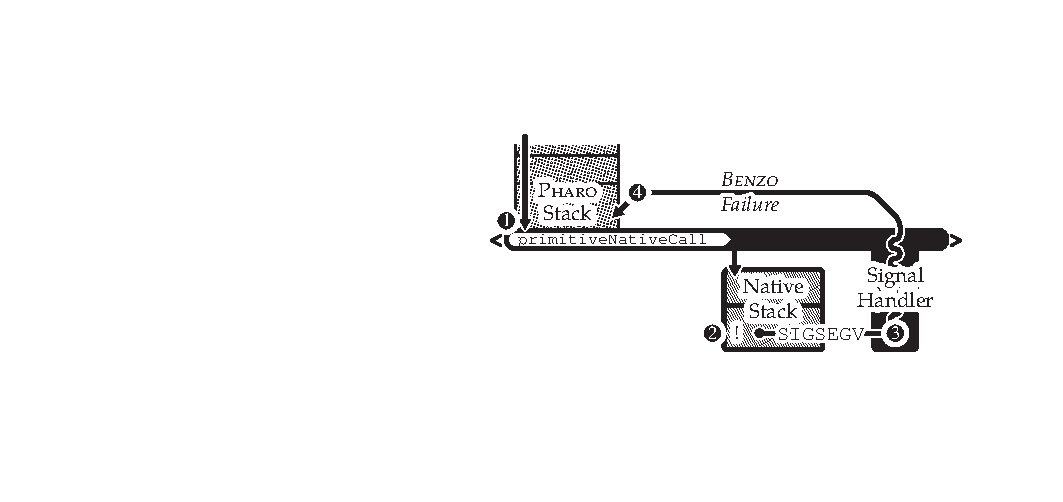
\includegraphics[scale=\imagescale]{benzo-debugger}
	\caption{\B Debugger Outline}
	\figlabel{benzo-debugger}
\end{figure}

The following list explains the detailed steps of \figref{benzo-debugger}.
\todo{missing link from the text}
\begin{enumerate}
	\item Standard \PH method activating a \B-enabled method through the \ttt{primitiveNativeCall} primitive.
	\item Native code causing a memory access violation (for example \ttt{SIGSEV}) which can not be handled by \PH directly.
	\item Low-level signal handler is activated by the operating system and tries to walk back the native stack up to the \ttt{primitiveNativeCall} activation.
	\item After successfully finding the \ttt{primitiveNativeCall} the signal handler sends a \B failure back to \PH.
\end{enumerate}

\noindent We assume that with the outlined mechanism an important fraction of the occurring memory access violations could be handled adequately in \PH.
However, since there is no real protection in the native code, there is no guarantee that the main \PH \VM can continue working.
Faulty native code might have corrupted the main \PH stack or heap beyond repair.
Nevertheless, this scheme could bring approximate a \PH like user experience for native \B code.
\sm{Instead of Pharo -> high level (again, this is one of your thesis goals, your thesis goal is not improving Pharo, but to contribute to the global set of knowledge)}


% -----------------------------------------------------------------------------
\subsection{Platform Independence}
\seclabel{benzo-problems-platform-independence}
% -----------------------------------------------------------------------------
The previous two issues discussed, robustness and debuggability, both target the integration into the existing \PH development environment.
This third issue on the other hand is related to the system integration: platform independence.

The \textsc{Intel x86} instruction set is widely distributed and supported by a variety of operating systems and thus the primary choice as native backend for \B.
Since the generated code is independent of C functions it works on all platforms with x86 support.
However, other architectures such as \ARM start to be more widespread and inevitable \B has to be ported on other platforms.
%A prominent example are \textsc{Apple}'s tablets and mobile phones running iOS.
In contrast to \PH itself, \B does not work on \ARM platform since all the low-level code is written in terms of x86 instructions.
While there is no way around a \ARM version of the underlying assembler, we think that porting all existing \B routines is too costly.
Instead we suggest to use an intermediate format that is platform independent more high-level than direct assembler instructions.
We call this intermediate format \VCPU and it has the following properties:
%
\begin{itemize}[noitemsep]
	\item High-level three-address-code (\TAC) instructions
	\item Automatic stack-management
\end{itemize}
%
Along with the ongoing work for this thesis we already started implementing \VCPU as a fork of the original compiler infrastructure of the \P \VM.
\sm{What is this? Why is that discussed here, and not integrated with the whole benzo story? If you got the design, and a more or less working solution sell it as key aspect!

That is eh solution you envision, in the limitations section you can then clarify that virtualcpu is buggy, or only partially implemented, so that you bypass it for many things...(well, if virtualcpu has sufficient maturity, but i }

\paragraph{\VCPU}
\seclabel{benzo-problems-vcpu}
In this following paragraph we are going to highlight the benefits and usage of \ugh{this intermediate format}.
\VCPU is based on a \TAC to simplify the adoption of optimizations such as \SSA.
These \TAC instructions take the following form:
%
\begin{stcode}{}
result := argument1 OP argument2
\end{stcode}
%
There are three operands involved, \ttt{result}, \ttt{argument1} and \ttt{argument2}, from which the name of this instruction format originates.
Based on this assumption, each standard \VCPU instruction returns a temporary variable which can be used for further operations.
The following code example outlines the basic usage of \VCPU:
%
\begin{stcode}[
	label={lst:benzo-problem-vcpu}, 
	caption={Basic \VCPU Example}
]{}
Benzo vcpu x86 generate: [ :asm | | temp1 temp2 |
	temp1 := asm memoryAt: 16r12345.
	temp2 := asm uint: 2.
	asm return: temp1 + temp1 ]
\end{stcode}
%
Which corresponds to the same functionality expressed in the following x86 instructions:
%
\begin{stcode}{}
Benzo x86 generate: [ :asm |
	asm mov: 16r12345 ptr to: asm EAX.
	asm add: asm EAX with: 2.
	asm return ]
\end{stcode}
%
To get to the final native instructions the \VCPU infrastructure compiles the high-level instructions to the specific backend.
The current compiler is divided into the following passes:
%
\begin{itemize}[noitemsep]
\item Platform Specific Transformation
\item Register Allocation
\item Superfluous Assignment Remover
\item Platform Specific Assembler
\end{itemize}
%
Applying these compiler passes to the example in \lstref{benzo-problem-vcpu} yields the following native instructions:
%
\begin{stcode}{}
mov   6 -> EDX
mov   2 -> ECX
add EDX,   ECX
mov ECX -> EAX
return 
\end{stcode}


\noindent With a properly parametrized register allocator and a separate constant folding pass the result could be greatly improved.
%A more detailed motivation and implementation details of this compiler are given in the following \secref{future-mate-compiler}.

% ===========================================================================
\section{Conclusion and Summary}
\seclabel{benzo-conclusion}
% ===========================================================================

In this chapter we presented \B, an integral approach for reflective high-level low-level programming.
\B consists of three core parts: \AsmJIT a language-side assembler, a set of primitives to activate native code and language-side library to handle dynamic code installation and activation.

\B promotes a smooth and powerful interaction with the low-level world by dynamically generating native code from language-side.
This enables to exploit the underlying platform capabilities when strongly needed without leaving the host development platform.
Most of the \B infrastructure is implemented at language-side and thus susceptible to modification. 
As a result, \B advocates the use of development tools and abstraction level of the high-level language for as much as possible or desired.

\paragraph{\B Applications}
Based on \B we outlined in this chapter three example applications: an \FFI in \secref{benzo-ffi}, dynamic primitives in \secref{benzo-waterfall} and a language-side \JIT compiler in \secref{benzo-nabujito}.
Typically all these applications require either a modified \VM or a dedicated plugin while our implementations are based on a central framework for low-level interaction.
In this chapter we only outlined these application to stress the fact that they use \B and only the following chapters will shed light on the implementation details of these three applications.

\paragraph{\B Performance}
Using the three \B-based applications we evaluate the performance of \B compare to a typical \VM-level implementation.
In summary we note that \B's code generation at language-side is slow compared to a single invocation the final native code.
However, this is only a one-time overhead since \B caches native code transparently at language-side.
Additionally we generate specific native code for each different application we easily outperform a static solution.
This becomes evident with the \FFI implementation that is based on \B.
Our mature \FFI implementation outperforms an existing C-\FFI implementation by a factor of 1.5 even though we control every aspect from language-side.

By combining high-level reflection capabilities with efficient low-level code we manage to do dynamic primitive instrumentation and reuse the code for primitive operations which is duplicated on the standard \JIT approach.
We also show that since our \JIT compiler poses only a one-time overhead when generating native code. 

\paragraph{\B's Limitiations}
Even though \B allows us to implement the three example applications at language-side, the complete development interaction requires improvement.
Currently there is not protection against faulty assembler code nor support for a low-level debugger.
To clearly support the theory of boundary-less low-level interaction a basic debugging infrastructure is required as outlined in \secref{benzo-problems}.

\paragraph{\B Outlook}
\B shows that promoting clear interfaces for controlling low-level code completely from language-side produces efficient solutions for system programming without resorting to pure low-level solutions.
Our set of \B-based applications shows that it our approach is feasible and efficient.
At the first sight \B is a simple application to invoke native code but we think that it opens doors for a new kind of language runtime.
In this envisioned system there is no longer a clear barrier between \VM and language-side.
This might seem far fetched but becomes more apparent when having a look at the \JIT of \PH which reimplements a performance critical set of primitives in its own native code.
Essentially this is code duplication since the primitives already exist as normal C code in the \VM sources.
With \B and the described dynamic primitives we should reuse the same code base for creating the \JIT representation of the primitive.\\

\noindent After presenting the basis of our high-level low-level programming framework in \PH we will focus on its application in the following chapters.


% =============================================================================
% empty version for the main document, where all the chapters are compiled together
\documentclass[a4paper,10pt,twoside]{../includes/ThesisStyle}
\usepackage[utf8]{inputenc}
\usepackage[T1]{fontenc}

\usepackage[left=1.5in,right=1.3in,top=1.1in,bottom=1.1in,includefoot,includehead,headheight=13.6pt]{geometry}\renewcommand{\baselinestretch}{1.05}


% =============================================================================
%\usepackage[sectionbib]{chapterbib}	% Cross-reference package (Natural BiB)
%\usepackage{bibunits}
%\usepackage{natbib}					% Put References at the end of each chapter
\usepackage{algorithm}
\usepackage{alltt}
\usepackage{amsfonts}
\usepackage{amsmath}
\usepackage{amssymb}
\usepackage{cite}
\usepackage{color}
\usepackage{enumerate}
\usepackage{fancyhdr}					% Fancy Header and Footer
\usepackage{graphicx}
\usepackage{ifthen}
\usepackage{latexsym}
\usepackage{multirow}
\usepackage{rotating}					% Sideways of figures & tables
\usepackage{stmaryrd}
\usepackage{subfigure}
\usepackage{url}         
\usepackage{xspace}

\usepackage[a4paper,pagebackref,hyperindex=true]{hyperref}
        

% =============================================================================

% Table of contents for each chapter
\usepackage[nottoc, notlof, notlot]{tocbibind}
\usepackage{minitoc}
\setcounter{minitocdepth}{1}
\mtcindent=15pt

\setcounter{secnumdepth}{3}
\setcounter{tocdepth}{2}
  
% =============================================================================
% Fancy Header Style Options

\pagestyle{fancy}                       % Sets fancy header and footer
\fancyfoot{}                            % Delete current footer settings

%\renewcommand{\chaptermark}[1]{         % Lower Case Chapter marker style
%  \markboth{\chaptername\ \thechapter.\ #1}}{}} %

%\renewcommand{\sectionmark}[1]{         % Lower case Section marker style
%  \markright{\thesection.\ #1}}         %

\fancyhead[LE,RO]{\bfseries\thepage}    % Page number (boldface) in left on even
% pages and right on odd pages
\fancyhead[RE]{\bfseries\nouppercase{\leftmark}}      % Chapter in the right on even pages
\fancyhead[LO]{\bfseries\nouppercase{\rightmark}}     % Section in the left on odd pages

\let\headruleORIG\headrule
\renewcommand{\headrule}{\color{black} \headruleORIG}
\renewcommand{\headrulewidth}{1.0pt}
\usepackage{colortbl}
\arrayrulecolor{black}

\fancypagestyle{plain}{
  \fancyhead{}
  \fancyfoot{}
  \renewcommand{\headrulewidth}{0pt}
}


% =============================================================================
% Clear Header Style on the Last Empty Odd pages
\makeatletter

\def\cleardoublepage{\clearpage\if@twoside \ifodd\c@page\else%
  \hbox{}%
  \thispagestyle{empty}%              % Empty header styles
  \newpage%
  \if@twocolumn\hbox{}\newpage\fi\fi\fi}

\makeatother

\newenvironment{maxime}[1]
{
\vspace*{0cm}
\hfill
\begin{minipage}{0.5\textwidth}%
%\rule[0.5ex]{\textwidth}{0.1mm}\\%
\hrulefill $\:$ {\bf #1}\\
%\vspace*{-0.25cm}
\it 
}%
{%

\hrulefill
\vspace*{0.5cm}%
\end{minipage}
}

\let\minitocORIG\minitoc
\renewcommand{\minitoc}{\minitocORIG \vspace{1.5em}}


\renewcommand{\epsilon}{\varepsilon}

% centered page environment
\newenvironment{vcenterpage}
	{\newpage\vspace*{\fill}\thispagestyle{empty}\renewcommand{\headrulewidth}{0pt}}
	{\vspace*{\fill}}
	
	
% =============================================================================
\newboolean{showcomments}
\setboolean{showcomments}{true}

\ifthenelse{\boolean{showcomments}} {
	\newcommand{\ugh}[1] {\textcolor{red}{\uwave{#1}}}	% please rephrase
	\newcommand{\ins}[1] {\textcolor{blue}{\uline{#1}}}	% please insert
	\newcommand{\del}[1] {\textcolor{red}{\sout{#1}}}	% please delete
	\newcommand{\chg}[2] {								% please change
		\textcolor{red}{\sout{#1}}{\ra}
		\textcolor{blue}{\uline{#2}}}
	\newcommand{\nbc}[3]{								% comment
		{\colorbox{#3}{\bfseries\sffamily\scriptsize\textcolor{white}{#1}}}
		{\textcolor{#3}{\sf\small$\blacktriangleright$\textit{#2}$\blacktriangleleft$}}}

}{
	\newcommand{\ugh}[1]{#1}							% please rephrase
	\newcommand{\ins}[1]{#1}							% please insert
	\newcommand{\del}[1]{}								% please delete
	\newcommand{\chg}[2]{#2}							% please change
	\newcommand{\nbc}[3]{}								% comment
}

% =============================================================================
\usepackage[a4paper,pagebackref,hyperindex=true]{hyperref}


% Links in pdf
\usepackage{color}
\definecolor{linkcol}{rgb}{0.0, 0.0, 0.0} 
\definecolor{citecol}{rgb}{0.0, 0.0, 0.0} 

% Change this to change the informations included in the pdf file
% See hyperref documentation for information on those parameters
\hypersetup {
	bookmarksopen=true,
	pdftitle="Design and Use of Anatomical Atlases for Radiotherapy",
	pdfauthor="Olivier COMMOWICK", 
	pdfsubject="Creation of atlases and atlas based segmentation", %subject of the document
	%pdftoolbar=false, % toolbar hidden
	pdfmenubar=true, %menubar shown
	pdfhighlight=/O, %effect of clicking on a link
	colorlinks=true,
	pdfpagemode=None,
	pdfpagelayout=SinglePage,
	pdffitwindow=true,
	linkcolor=linkcol,
	citecolor=citecol,
	urlcolor=linkcol
}

% =============================================================================
\newcommand{\figlabel}[1]{\label{fig:#1}}
\newcommand{\seclabel}[1]{\label{sec:#1}}
\newcommand{\tablabel}[1]{\label{tab:#1}}

\newcommand{\figref}[1]{Figure~\ref{fig:#1}}
\newcommand{\secref}[1]{Section~\ref{sec:#1}}
\newcommand{\tabref}[1]{Table~\ref{tab:#1}}

\newcommand{\commented}[1]{}

\newcommand{\eg}{\emph{e.g.,}\xspace}
\newcommand{\ie}{\emph{i.e.,}\xspace}


\newcommand\fix[1]{\nb{FIX}{#1}}
\newcommand\todo[1]{\nb{TO DO}{#1}}

% =============================================================================

\graphicspath{{.}{../figures/}}

\begin{document}
% =============================================================================

\chapter{Validation: FFI}
\chaplabel{ffi}
\minitoc

% ===========================================================================
\section{Introduction}
\seclabel{introduction}
% ===========================================================================

\begin{figure*}[ht]
	\centering
	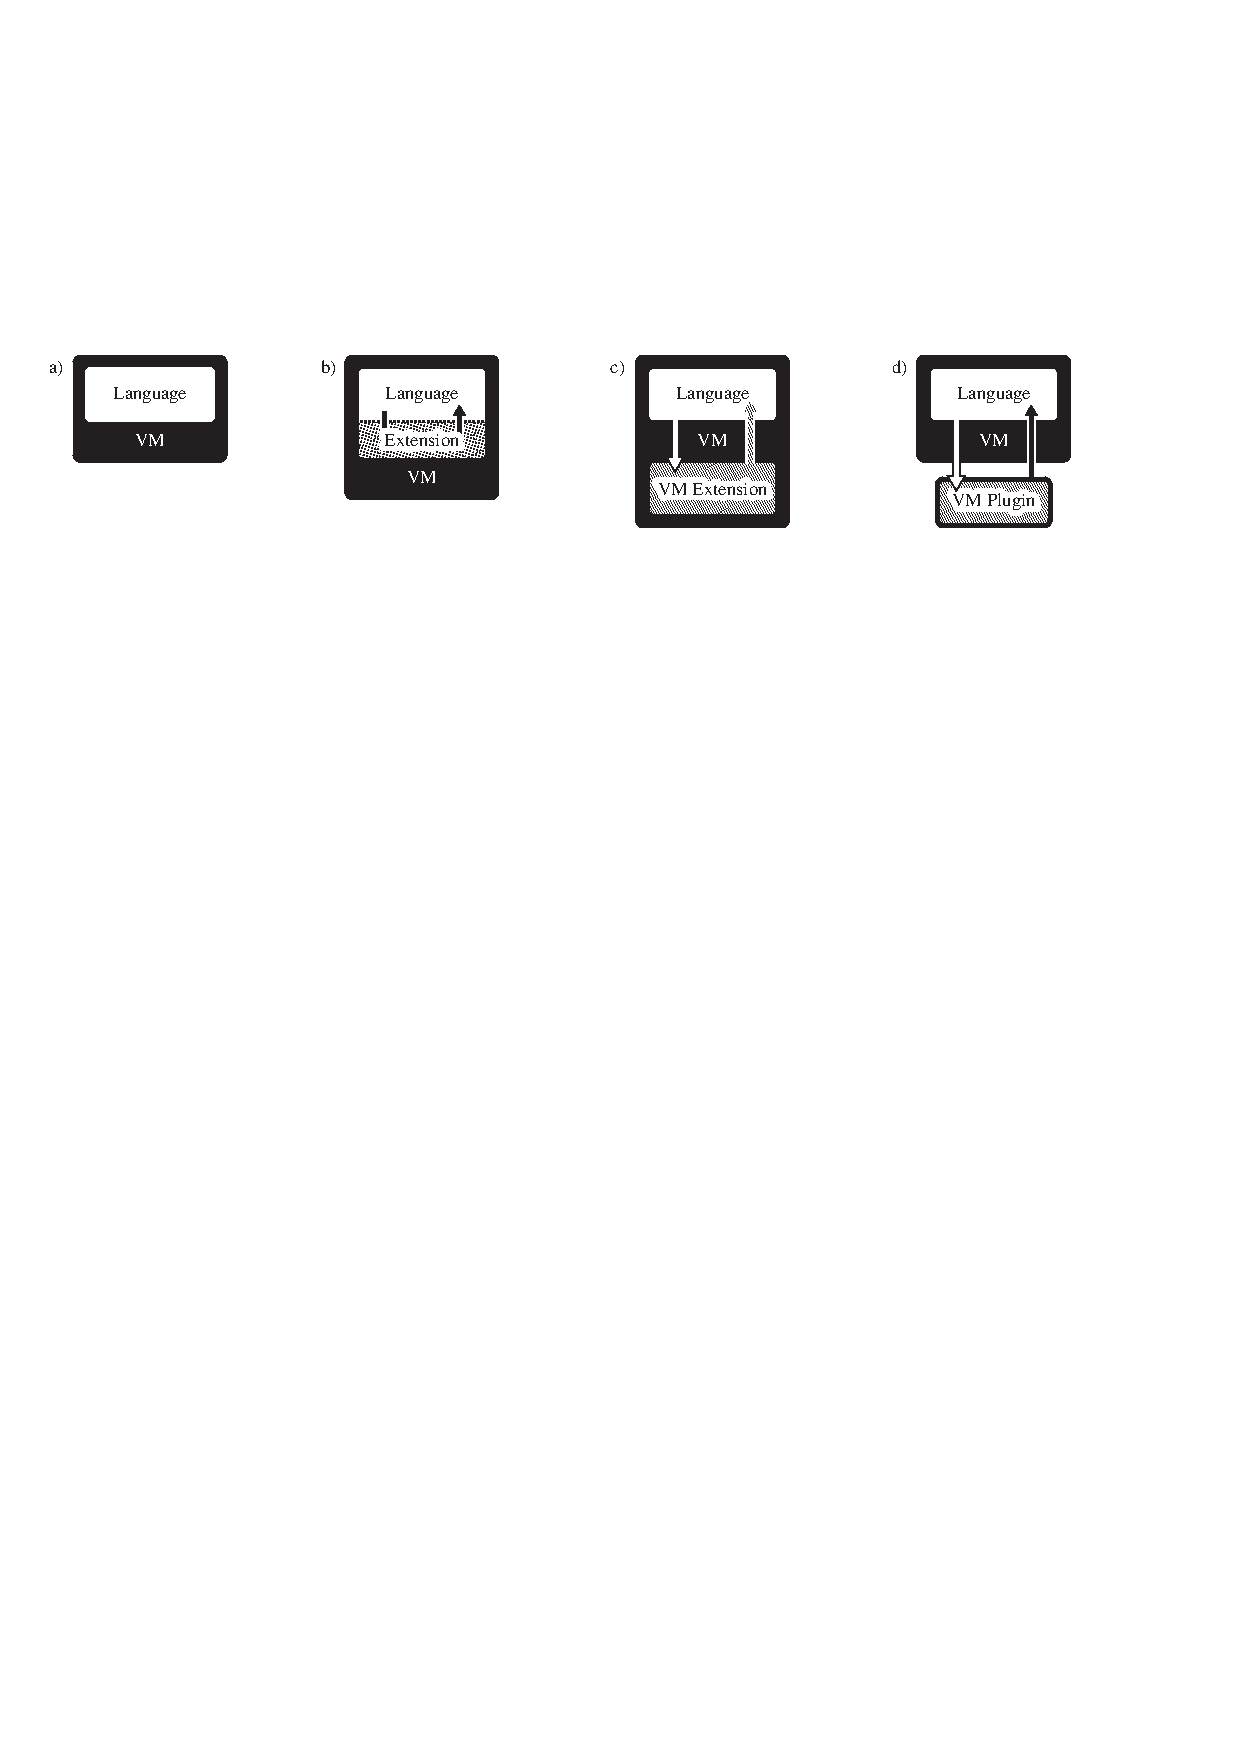
\includegraphics[width=\textwidth]{extensionComparison}
	\caption{Comparing different extension mechanisms: a) library implemented completely at language-side running on a standard VM, b) language using features from a VM extension, c) language using features from a VM plugin, d) language-side implementation of an extension.}
	\figlabel{extensionComparison}
\end{figure*}

Currently, more and more code is produced and available through reusable libraries such as OpenGL\footnote{\url{http://www.opengl.org/}} or Cairo\footnote{\url{http://cairographics.org/}}.
While working on your own projects using dynamic languages, it is crucial to be able to use such existing libraries with little effort.
Multiple solutions exist to achieve access to an external library from dynamic languages that are executed on the top of a virtual machine (VM) such as Pharo\footnote{\url{http://pharo.org/}}, Lua\footnote{\url{http://lua.org/}} or Python\footnote{\url{http://python.org/}}.
Figure~\figref{extensionComparison} depicts four possibilities of dealing with new or external libraries in a high-level language.

\paragraph{Language-side Library.}
One solution is to re-implement a library completely at language-side (cf. Figure~\figref{extensionComparison}.a).
Even though this is the most flexible solution, this is often not an option, neither from the technical point of view (performance penalty), nor from the economic point of view (development time and costs).

\paragraph{VM Extension.}
The second one (\figref{extensionComparison}.b) is to do a \emph{VM extension} providing new primitives that the high-level language uses to access the native external library.
This solution is generally efficient since the external library may be statically compiled within the VM.
However a tight integration into the VM also means more dependencies and a different development environment than the final product at language-side.

\paragraph{VM Plugin.}
The third solution (\figref{extensionComparison}.c) is similar to the previous one but the extension is factored out of the VM as a \emph{plugin}.
This solution implies again a lot of low-level development at VM-level that must be done for each external library we want to use.
Additionally we have to adapt the plugin for all platforms on which the VM is supposed to run on.

\paragraph{FFI.}
A higher-level solution is to define \emph{Foreign Function Interfaces} (FFIs) (cf. Figure~\figref{extensionComparison}.d).
The main advantage of this approach is that once a VM is FFI-enabled, only a language extension (no VM-level code) is needed to provide access to new native libraries.
From the portability point of view, only the generic FFI VM-plugin has to be implemented on all platforms.

% Challenges & Goals
Implementing an FFI library is a challenging task because of its antagonist goals:
\begin{itemize}
    \item it must be flexible enough to easily bind to external libraries and also express complex foreign calls regarding the memory management or the type conversions (marshalling);
    \item it must be well integrated with the language (objects, reflection, garbage collector);
    \item it must be efficient.
\end{itemize}
%
Existing FFI libraries of dynamic languages all have different designs and implementations because of the trade-offs they made regarding these goals and challenges.
Typical choices are resorting purely to the VM-level and thus sacrificing flexibility.
The inverse of this approach exists as well: FFIs can be implemented almost completely at language-side but at a significant performance loss.
Both these pitfalls are presented in more detail in Section~\secref{evaluation}.


% list shortcomings of typical implementations (C-FFI vs ALIEN)
% - too low-level (C-FFI) fast in simple examples, complex calls not possible
% - too high-level (ALIEN) slow in simple examples, quite slow in complex ones
% - missing specific code generation
% - missing JIT interaction for speed (like LuaJIT, org.vmmagic)

% Alien and C-FFI run in the same Pharo image as NativeBoost allowing a much closer comparison.
% Alien FFI is implemented almost completely at language-side, much like NativeBoost. However, as the following benchmarks will stress, it also suffers from performance loss.
% On the other end there is C-FFI which is faster than Alien but by far not as flexible. For instance only primitive types are handled directly.


This paper presents \NBFFI\footnote{\url{http://code.google.com/p/nativeboost}} an FFI library at language-side for Pharo that supports callouts and callbacks, which we present in Section~\secref{nutshell}.
There are at least two other existing FFI libraries in Pharo worth mentioning: C-FFI and Alien.
Nevertheless, they both present shortcomings.
C-FFI is fast because it is mostly implemented at VM-level, however it is limited when it comes to do complex calls that involve non-primitive types or when we want to define new data types.
On the opposite, Alien FFI is flexible enough to define any kind of data conversion or new types directly at language-side but it is slower than C-FFI because it is mostly implemented at language-side.
In essence, \NBFFI combines the flexibility and extensibility of Alien that uses language-side definition for marshalling and the speed of C-FFI which is implemented at VM-level.
The main originalities of \NBFFI are:

\begin{description}
	\item[Extensibility.] \NBFFI relies on as few VM primitives as possible (5 primitives), essentially to call native code.  Therefore, most of the implementation resides at language-side, even low-level mechanisms. That makes \NBFFI easily extensible because its implementation can be changed at any time, without needing to update the runtime (VM). It also presents a noticeable philosophical shift, how we want to extend our language in future. A traditional approach is to implement most low-level features at VM-side and provide interfaces to the language-side.
But that comes at cost of less flexibility and longer development and release cycles. On the opposite, we argue that extending language features, even low-level ones, should be done at language-side instead. This results in higher flexibility and without incurring high runtime costs which usually happen when using high-level languages such as Smalltalk.
	\item[Language-side extension.] Accessing a new external library using \NBFFI involves a reduced amount of work since it is only a matter of writing a language-side extension.
	\item[Performance.] Despite the fact it is implemented mostly at language-side, \NBFFI achieves superior performance compared to other FFI implementations running Pharo.
    This is essentially because it uses automatic and transparent native code generation at language-side for marshalling.
\end{description}

%In the following section we present the language-side code that one should write to achieve to interact with external libraries with \NBFFI.
%We then compare performance of \NBFFI with three other FFI implementations in Section~\secref{evaluation}.
%The following Section~\secref{internals} gives more insights on the \NB.
%After the related work presented in Section~\secref{relatedWork} and we conclude this paper in Section~\secref{conclusion}.


% ===========================================================================
\section{\NBFFI: an Introduction}
\seclabel{nutshell}
% ===========================================================================

This section gives an overview of the code that should be written at language-side
to enable interactions with external libraries.

\subsection{Simple Callout}

Listing~\lstref{clock} shows the code of a regular Smalltalk method named \ttt{ticksSinceStart} that defines a callout to the \ttt{clock} function of the \texttt{libc}.
\NB imposes no constraint on the class in which such a binding should be defined.
However, this method must be annotated with a specific pragma (such as \ttt{<primitive:module:>}) which specifies that a native call should be performed using the \NB plugin.

\begin{stcode}[
	label={lst:clock},
	caption={\NBFFI example of callout declaration to the \ttt{clock} function of the \texttt{libc}}]{0}
ticksSinceStart
	<primitive: #primitiveNativeCall
	 module: #NativeBoostPlugin>
	^ self
		nbCall: #(uint clock ())
		module: NativeBoost CLibrary
\end{stcode}

The external function call is then described using the \ttt{nbCall:module:} message.
The first parameter (\ttt{\#nbCall:}) is an array that describes the signature of C function to callout.
Basically, this array contains the description of a C function prototype, which is very close to normal C syntax.
The return type is first described (\ttt{uint} in this example\footnote{The return type of the \texttt{clock} function is \ttt{clock\_t}, but we deliberately used \ttt{uint} in this first example for the sake of simplicity even if it is possible to define a constant type in \NB.}), then the name of the function (\ttt{clock}) and finally the list of parameters (an empty array in this example since \ttt{clock} does not have any).
The second argument, \ttt{\#module:} is the module name, its full path or its handle if already loaded, where to look up the given function.
This example uses a convenience method of \NB named \ttt{CLibrary} to obtain a handle to the standard C library.

% ===========================================================================
\subsection{Callout with Parameters}

% - explain argument detection (match var names)
Figure~\figref{nativeBoostSyntax} presents the general syntax of \NBFFI through an example of a callout to the \ttt{abs} function of the \texttt{libc}.
The \ttt{abs:} method has one argument named \ttt{anInteger} (cf. \ding{182}).
This method uses the pragma \ttt{<primitive:module:error:>} which indicates that the \texttt{\#primitiveNativeCall} of the \texttt{\#NativeBoostPlugin} should be called when this method is executed (cf. \ding{183}).
An \texttt{errorCode} is returned by this primitive if it fails and the regular Smalltalk code below is executed (cf. \ding{184}).
The main difference with the previous example is that the \texttt{abs} function takes one integer parameter.
In this example, the array \texttt{\#(uint abs(int anInteger))} passed as argument to \texttt{\#nbCall:} contains two important information (cf. \ding{185}).
First, the types annotations such as the return type (\texttt{uint} in both examples) and arguments type (\texttt{int} in this example).
These types annotations are then used by \NBFFI to automatically do the marshalling between C and Pharo values as illustrated by the next example.
Second, the values to be passed when calling out.
In this example, \texttt{anInteger} refers to the argument of the \ttt{abs} method, meaning that the value of this variable should be passed to the \texttt{abs} C function.
Finally, this \texttt{abs} function is looked up in the \texttt{libc} whose an handle is passed in the \texttt{module:} parameter (cf. \ding{186}).
% A library can be designated either by its file path on disk or its memory address.
% \begin{stcode}[
% 	label={lst:abs},
% 	caption={Example of callout to the \ttt{abs} function}]{0}
% abs: anInteger
% 	<primitive: #primitiveNativeCall
% 	 module: #NativeBoostPlugin>
%
% 	^ self
% 		nbCall: #(uint abs(int anInteger))
% 		module: NativeBoost CLibrary
% \end{stcode}
%
% - explain syntax in picture (line plus arrows)
\begin{figure}[H]
	\centering
	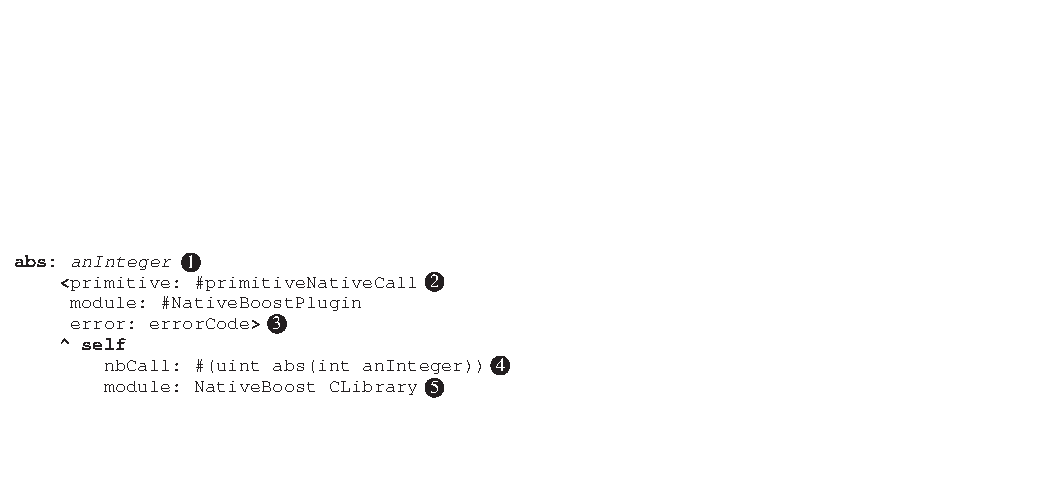
\includegraphics{nativeBoostSyntax}
	%\nocaptionrule
	%\captionsetup{singlelinecheck=off}
	\caption[\NB basic method]{Example of the general \NBFFI callout syntax}
	\figlabel{nativeBoostSyntax}
\end{figure}

% ===========================================================================
\subsection{Automatic Marshalling of Known Types}

Listing~\lstref{getenv} shows a callout declaration to the \texttt{getenv} function that takes one parameter.

\begin{stcode}[
	label={lst:getenv},
	caption={Example of callout to \ttt{getenv}}]{0}
getenv: name
	<primitive: #primitiveNativeCall
	 module: #NativeBoostPlugin>

	^ self
		nbCall: #(String getenv(String name)
		module: NativeBoost CLibrary
\end{stcode}

In this example, the \NB type specified for the parameter is \texttt{String} instead of \texttt{char*} as specified by the standard \texttt{libc} documentation.
This is on purpose because strings in C are sequences of characters (\ttt{char*}) but they must be terminated with the special character: \cnull.
Specifying \texttt{String} in the \texttt{\#nbCall:} array will make \NB to automatically do the arguments conversion from Smalltalk strings to C strings (\cnull terminated \texttt{char*}).
It means that the string passed will be put in an external C \ttt{char} array and a \cnull character will be added to it at the end.
This array will be automatically released after the call returned.
This is an example of automatic memory management of \NB that can also be controlled if needed.
Obviously, the opposite conversion happens for the returned value and the method returns a Smalltalk String.
This example shows that \NBFFI accepts literals, local and instance variable names in callout declarations and it uses their type annotation to achieve the appropriate data conversion.
Table~\tabref{nbPrimitiveTypes} shows the default and automatic data conversions achieved by \NBFFI.

\begin{table}[hbt]
    \centering
    \begin{tabular}{rll}
        Primitive Type       & Smalltalk Type \\\midrule
        \ttt{uint}   & \ttt{Integer} \\
        \ttt{int}    & \ttt{Integer} \\
        \ttt{String} & \ttt{ByteString} \\
        \ttt{bool}   & \ttt{Boolean} \\
        \ttt{float}  & \ttt{Float} \\
        \ttt{char}   & \ttt{Character} \\
        \ttt{oop}    & \ttt{Object}
    \end{tabular}
    \caption{Default \NBFFI mappings between C/primitive types and high-level types. Note that \ttt{oop} is not a real primitive type as no marshalling is applied and the raw pointer is directly exposed to Pharo.}
    \tablabel{nbPrimitiveTypes}
\end{table}
Listing~\lstref{setenv} shows another example to callout the \texttt{setenv} function.
The return value will be converted to a Smalltalk \texttt{Boolean}.
The two first parameters are specified as \texttt{String} and will be automatically transformed in \texttt{char*} with an ending \cnull character.
The last parameter is \texttt{1}, a Smalltalk literal value without any type specification and \NB translates it as an \texttt{int} by default.

\begin{stcode}[
	label={lst:setenv},
	caption={Example of callout to \ttt{setenv}}]{0}
setenv: name value: value
	<primitive: #primitiveNativeCall
	 module: #NativeBoostPlugin>

	^ self
		nbCall: #(Boolean setenv(String name,
								 String value,
								 1)
		module: NativeBoost CLibrary
\end{stcode}

Another interesting example of automatic marshalling is to define the \ttt{abs} method (cf. Figure~\figref{nativeBoostSyntax}) in the \ttt{SmallInteger} class and passing \texttt{self} as argument in the callout. In such case, \NB automatically converts \texttt{self} (which is a SmallInteger) into an \texttt{int}.
This list of mapping is not exhaustive and \NB also supports the definition of new data types and new conversions into more complex C types such as structures (cf. Section~\secref{internals}).



% memory alloc & structs
\begin{table}[t]
    \centering
    \begin{tabular}{lcccc}
                    &  Memory 	& Address & Marshalling & Constraint  \\\midrule
C-managed struct 	&  C heap  	& fixed & passed by reference & must be freed \\
Pharo-managed struct & Object memory & variable & passed by reference & may move \\
& & & or passed by copy & costly\\
    \end{tabular}
    \caption{Wrapping structures possibilities in \NB}
    \tablabel{wrappingstruct}
\end{table}

% ===========================================================================
\subsection{Supporting new types}\seclabel{newtypes}

The strength of language-side FFIs appears when it comes to do callouts with new data types involved.
\NBFFI supports different possibilities to interact with new types.

\paragraph{Declaring structures.}
For example, the Cairo library\footnote{\url{http://cairographics.org}} provides complex structures such as \texttt{cairo\_surface\_t} and functions to manipulate this data type. % which makes field access useless.
Listing~\lstref{AthensCairoSurface} shows how to write a regular Smalltalk class to wrap a C structure.
\NB only requires a class-side method named \texttt{asNBExternalType:} that describes how to marshall this type back and forth from native code.
In this example, we use existing marshalling mechanism defined in \texttt{NBExternalObjectType} that just copies the structure's pointer and stores it in an instance variable named \ttt{handle}.

\begin{stcode}[
	label={lst:AthensCairoSurface},
	caption={Example of C structure wrapping in \NB}]{0}
AthensSurface subclass: #AthensCairoSurface
	instanceVariableNames: 'handle'.

AthensCairoSurface class>>asNBExternalType: gen
	"handle iv holds my address (cairo_surface_t)"
	^ NBExternalObjectType objectClass: self
\end{stcode}

\paragraph{Callout with structures.}
Listing~\lstref{calloutOpaqueStruct} shows a callout definition to the \texttt{cairo\_image\_surface\_create} function that returns a \ttt{cairo\_surface\_t*} data type.
In this code example, the return type is \texttt{AthensCairoSurface} directly (not a pointer).
When returning from this callout, \NB creates an instance of \texttt{AthensCairoSurface} and the marshalling mechanism  stores the returned address in the \texttt{handle} instance variable of this object.

\begin{stcode}[
	label={lst:calloutOpaqueStruct},
	caption={Example of returning a structure by reference}]{0}
primImage: aFormat width: aWidth height: aHeight
	<primitive: #primitiveNativeCall
	 module: #NativeBoostPlugin
     error: errorCode>

	^self nbCall: #(AthensCairoSurface
		cairo_image_surface_create (int aFormat,
									int aWidth,
									int aHeight) )
\end{stcode}

Conversely, passing an \texttt{AthensCairoSurface} object as a parameter in a callout makes its pointer stored in its \texttt{handle} iv (cf. Listing~\lstref{calloutOpaqueStructParameter}) to be passed.
Since the parameter type is \ttt{AthensCairoSurface} in the callout definition, \NB also ensures that the passed object is really an instance of this class.
If it is not, the callout fails before executing the external function because passing it an address on a non-expected data could lead to unpredicted behavior.

\begin{stcode}[
	label={lst:calloutOpaqueStructParameter},
	caption={Example of passing a structure by reference}]{0}
primCreate: cairoSurface
	<primitive: #primitiveNativeCall
	 module: #NativeBoostPlugin>

	^self nbCall: #(
        AthensCairoCanvas cairo_create (
                  AthensCairoSurface cairoSurface))
\end{stcode}


\paragraph{Accessing structure fields.}
In \NB, one can directly access the fields of a structure if needed, even if it is not a good practice from the data encapsulation point of view.
Nevertheless, it may be mandatory to interact with some native libraries that do not provide all the necessary functions to manipulate the structure.
Listing~\lstref{cairo_c_definition} shows an example of a C struct type definition for \texttt{cairo\_matrix\_t}.

\begin{ccode}[
	label={lst:cairo_c_definition},
	caption={Example external type to convert back and forth with the Cairo library}]{0}
typedef struct {
    double xx; double yx;
    double xy; double yy;
    double x0; double y0;
} cairo_matrix_t;
\end{ccode}

Listing~\lstref{AthensCairoMatrix} shows that the \texttt{NBExternalStructure} of \NBFFI can be subclassed to define new types such as \texttt{AthensCairoMatrix}.
The description of the fields (types and names) of this structure is provided by the \texttt{fieldsDesc} method on the class side.
Given this description, \NB lazily generates field accessors on the instance side using the field names.

\begin{stcode}[
	label={lst:AthensCairoMatrix},
	caption={Example of \NBFFI definition of an \texttt{ExternalStructure}}]{0}
NBExternalStructure
    variableByteSubclass: #AthensCairoMatrix.

AthensCairoMatrix class>>fieldsDesc
	^ #(  double sx; double shx;
		  double shy; double sy;
		  double x; double y;  )
\end{stcode}

Listing~\lstref{cairoCallouts} shows a callout definition to the
 \texttt{cairo\_matrix\_multiply} function passing \texttt{self} as argument with the type \ttt{AthensCairoMatrix*}.
\NB handles the marshalling of this object to a struct as defined in the \texttt{fieldsDesc}.
% The interesting point is that the called function \ttt{cairo\_matrix\_multiply} stores its result in the first argument i.e. the receiver object.

\begin{stcode}[
	label={lst:cairoCallouts},
	caption={Example of callouts using \ttt{cairo\_matrix\_t}}]{0}
AthensCairoMatrix>>primMultiplyBy: m
	<primitive: #primitiveNativeCall
	 module: #NativeBoostPlugin
     error: errorCode>

"C signature"
"void cairo_matrix_multiply (
                     cairo_matrix_t *result,
                     const cairo_matrix_t *a,
                     const cairo_matrix_t *b );"
	^self nbCall: #(void   cairo_matrix_multiply
		(AthensCairoMatrix * self,
		AthensCairoMatrix * m ,
		AthensCairoMatrix * self ) )
\end{stcode}


\paragraph{Memory management of structures.}
Table~\tabref{wrappingstruct} shows a comparison between C-managed and Pharo-managed structures.
The first ones are allocated in the C heap.
Their addresses are fixed and they are passed by reference during a callout.
But the programmer must free them by hand when they are not needed.
The second ones are allocated in the Pharo object-memory.
Their addresses are variable since their enclosing object may be moved by the garbage collector.
They can either passed by copy which is costly or by reference.
Passing a reference may lead to problems is the C function stores the address and try to access it later on since the address may changed.


% ===========================================================================
\subsection{Callbacks}

\NB supports callbacks from native code.
This means it is possible for a C-function to call back into the Pharo runtime and activate code.
We will use the simple \ttt{qsort} C-function to illustrate this use-case.
\ttt{qsort} sorts a given array according to the results of a compare function.
Instead of using a C-function to compare the elements we will use a callback to invoke a Pharo block which will compare the two arguments.
%
\begin{stcode}[
	label={lst:calloutWithCallback},
	caption={Example of callout passing a callback for \ttt{qsort}}]{0}
bytes := #[ 120 12 1 15 ].
callback := QSortCallback on: [ :a :b |
				(a byteAt: 0) - (b byteAt: 0) ].

self ffiQSort: bytes
	 length: bytes size
	 compareWith: callback
\end{stcode}
%
Code \lstref{calloutWithCallback} shows the primary Pharo method for invoking \ttt{qsort} with a \ttt{QSortCallback} instance for the compare function.
In this example \ttt{qsort} will invoke run the Pharo code inside the callback block to compare the elements in the \ttt{bytes} array.

To define a callback in \NB we have to create a specific subclasses for each callback with different argument types.
%
\begin{stcode}[
	label={lst:callbackDefinition},
	caption={Example of callback definition}]{0}

NBFFICallback
    subclass: #QSortCallback.

NBFFICallback class>>signature
	^#(int (NBExternalAddress a, NBExternalAddress b))
\end{stcode}
%
Code \lstref{callbackDefinition} shows \ttt{QSortCallback} which takes two generic external addresses as arguments.
These are the argument types that are being passed to the sort block in Example \lstref{calloutWithCallback}.
%
\begin{stcode}[
	label={lst:qsort},
	caption={Example of callout passing a callback}]{0}
ffiQSort: base len: size compare: qsortCallback
	<primitive: #primitiveNativeCall
	 module: #NativeBoostPlugin>

	"C qsort signature"
	"void qsort(
		void *base,
		size_t nel,
		size_t width,
		int (*compar)(const void *, const void *));"

	^ self
		options: #( optMayGC )
		nbCall: #(void qsort (
					NBExternalAddress array,
					ulong size,
					1, "sizeof an element"
					QSortCallback qsortCallback))
		module: NativeBoost CLibrary
\end{stcode}
%
The last missing piece in this example is the callout definition shown in Code \lstref{qsort}.
The \NB callout specifies the callback arguments by using \ttt{QSortCallback}.

%\begin{enumerate}
%	\item Define a callback by subclassing NBCallback and overriding \ttt{\#fnSpec} method that defines de C signature of the callback
	% Redefining callback signature.
% A callback uses a lazy-initialization scheme to generate a common marshalling code which will be used by all instances of specific callback class.
% So, changing a callback signature (by changing its #fnSpec method) will not have an immediate effect, if you already created at least a single instance of it.
% To make changes take effect, you must restart an image.

%	\item Define a callout as previously but passing a callback as argument using its class name as argument type.

% !!Note!! A special care must be taken for all functions which may make callbacks!
% In the above qsort() example, you can see an additional option for external call - #optMayGC, which tells a code generator to call an external function via call gate (a special stub which handling a code relocation caused by GC). Thats it, for any external functions, which may call the callback you must pass this option.
% Rationale: since most of external functions don't make any callbacks (and so has no chance to trigger GC), using this option by default will be an overkill, which will just spend extra CPU cycles for nothing.
% However, if you omit this option when calling the function(s) which may call back, expect a hard crash(es) to happen.

%	\item instantiate the callback giving it a block.
	% To use callbacks, you must instantiate it first by passing block as an argument:
% mycallback := MyCallback on: someBlock.

% The block is the closure which will be evaluated when callback function get called, so the block must take same number of arguments as specified in #fnSpec method, and its evaluation result must yield a value which can be converted back C type value, which you speficied as a return type of callback function.
% For example, if callback signature is 'int (int foo , float bar )' , we can create a callback with following block closure:

% mycallback := MyCallback on: [:foo :bar |  (foo + bar ) asInteger ].


\paragraph{Callback lifetime.}
Each time a new callback is instantiated it reserves a small amount of external memory which is freed once the callback is no longer used.
This is done automatically using object finalization hooks..


% ===========================================================================
\subsection{Overview of \NBFFI Internals}
% - explain how code is generated in simple steps, not going into details

This section provides an overview of the internal machinery of \NBFFI though it is not mandatory to know it in order to use it as demonstrated by previous examples.

\paragraph{General Architecture.}
Figure~\figref{nbArchitecture} describes the general architecture of \NB.
Most code resides at language-side, nevertheless some generic extensions (primitives) to the VM are necessary to activate native code.
At language-side, callouts are declared with \NBFFI which processes them and dynamically generates x86 native code using the \texttt{AsmJit} library.
This native code is responsible of the marshalling and calling the external function.
\NB then uses a primitive to activate this native code.

\begin{figure}[h]
	\centering
	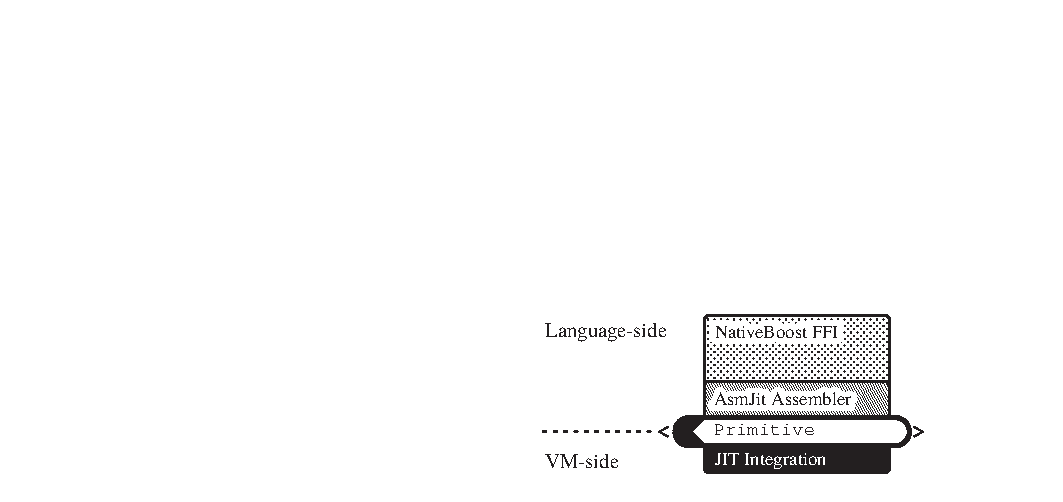
\includegraphics[scale=1.1]{nbArchitecture}
	\caption{\NB main components that major part of the code resides at language-side.}
	\figlabel{nbArchitecture}
\end{figure}

% General FFI overview and difference of NB
\begin{figure*}[t]
	\centering
	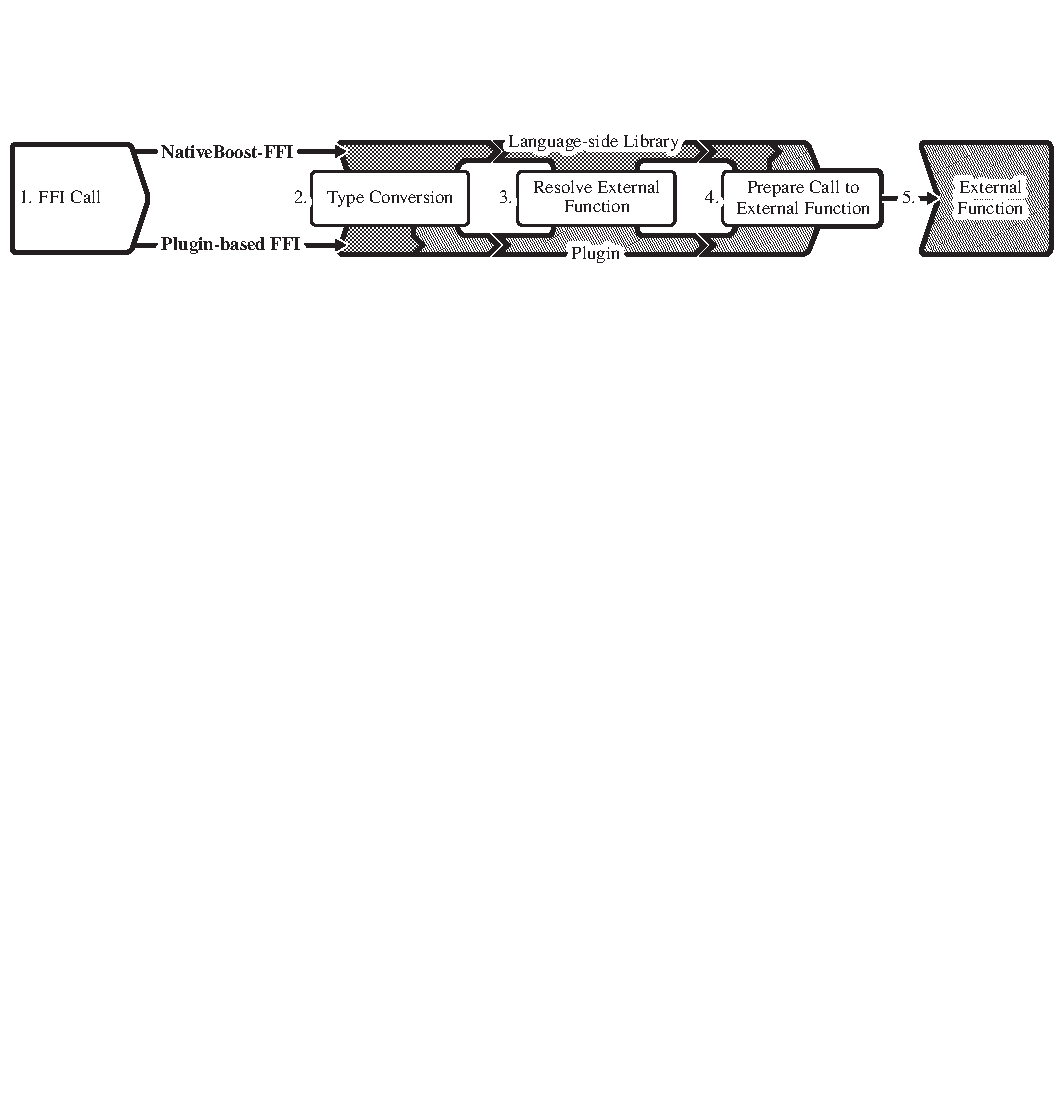
\includegraphics[width=\textwidth]{ffiOverview}
	\caption{Comparison of FFI calls propagation in \NBFFI and a typical VM plugin-based implementation. \NB resorts to VM-level only for the native-code activation, whereas typical implementations cross this barrier much earlier.}
	\figlabel{ffi}
\end{figure*}

\paragraph{Callout propagation.}
Figure~\figref{ffi} shows a comparison of the resolution of a FFI call both in \NBFFI and a plugin-based FFI.
At step 1, a FFI call is emitted.
The \NBFFI call is mostly processed at language-side and it is only during step 4 that a primitive is called and the VM effectively does the external call by executing the native code.
On the opposite, a plugin-based FFI call already crossed the low-level frontier in step 2 resulting that part of the type conversion process (marshalling) is already done in the VM code.
In \NBFFI, doing most of the FFI call processing at language-side makes easier to keep control, redefine or adapt it if needed.

% ===========================================================================
\section{\NBFFI Evaluation}
\seclabel{evaluation}
% ===========================================================================

In this section we compare \NB with other FFI implementations.
\begin{description}
	\item[Alien FFI:] An FFI implementation for Squeak/Pharo that focuses on the language-side. All marshalling happens transparently at language-side.
	\item[C-FFI:] A C based FFI implementation for Squeak/Pharo that performs all marshalling operations at VM-side.
	\item[LuaJIT:] A fast Lua implementation that has a close FFI integration with JIT interaction.
\end{description}

\paragraph{Choice of FFI Implementations.}
To evaluate \NB we explicitly target FFI implementations running on the same platform, hence we can rule out additional performance differences.
Alien and C-FFI run in the same Pharo image as \NB allowing a much closer comparison.

Alien FFI is implemented almost completely at language-side, much like \NB.
However, as the following benchmarks will stress, it also suffers from performance loss.

On the other end there is C-FFI which is faster than Alien but by far not as flexible. For instance only primitive types are handled directly.

As the third implementation we chose Lua. Lua is widely used as scripting language in game development.
Hence much care has been taken to closely integrate Lua into C and C++ environments.
LuaJIT integrates an FFI library that generates the native code for marshalling and directly inlines C functions callout in the JIT-compiled code.

\paragraph{Evaluation Procedure.}
To compare the different FFI approaches we measure 100 times the accumulative time spent to perform $1'000'000$ callouts of the given function.
From the 100 probes we show the average and the standard deviation for a $68\%$ confidence interval in a gaussian distribution.
To exclude the calling and loop overhead we subtract from each evaluation the time spent in the same setup, but without the FFI call.
The final deviation displayed is the arithmetic average of the measured deviation of the base and the callout measurement.

The three Smalltalk FFI solutions (\NB, Alien, C-FFI) are evaluated on the very same Pharo 1.4 (version 14458) image on a Pharo VM (version of May 5. 2013).
For the Lua benchmarks we use LuaJIT 2.0.1.
The benchmarks are performed under the constant conditions on a MacBook Pro.
Even though a standalone machine could improve the performance we are only interested in the relative performance of each implementation.


\paragraph{Choice of Callouts.}
We chose a set of representative C functions to stress different aspects of an FFI implementation.
We start with simple functions that require little marshalling efforts and thus mainly focus on the activation performance and callout overhead.
Later we measure more complex C functions that return complex types and thus stress the marshalling infrastructure.

% ===========================================================================
\subsection{Callout Overhead}
The first set of FFI callouts show mainly the overhead of the FFI infrastructure to perform the callout.

For the first FFI evaluation we measure the execution time for a \ttt{clock()} callout.
The C function takes no argument and returns an integer thus guaranteeing a minimal overhead for marshalling and performing the callout.
%
\begin{table}[H]
    \centering
    \begin{tabular}{rlr}
                    & Call Time                        & Relative Time \\\midrule
        \NB         & \ttt{492.13} $\pm$ \ttt{0.73} ms  & $1.0 \times$ \\
        Alien       & \ttt{606.6 } $\pm$ \ttt{1.9 } ms  & $\approx 1.2\times$ \\
        C-FFI       & \ttt{541.77} $\pm$ \ttt{0.88} ms  & $\approx 1.1\times$ \\
        LuaJIT     & \ttt{343.0 } $\pm$ \ttt{1.2 } ms  & $\approx 0.7\times$
    \end{tabular}
    \caption{Speed comparison of an \ttt{uint clock(void)} FFI call (see Code~\lstref{clock}).}
    \tablabel{performance-clock}
\end{table}
%
\noindent \ttt{abs} is a about the same complexity as the \ttt{clock} function, however accepting a single integer as argument.
%
\begin{table}[h!]
    \centering
    \begin{tabular}{rlr}
                    & Call Time                        & Relative Time \\\midrule
        \NB         & \ttt{ 65.34 } $\pm$ \ttt{0.23 } ms  & $1.00 \times$ \\
        Alien       & \ttt{175.77 } $\pm$ \ttt{0.31 } ms  & $\approx 2.69\times$ \\
        C-FFI       & \ttt{148.77 } $\pm$ \ttt{0.21 } ms  & $\approx 2.27\times$ \\
        LuaJIT\tablefootnote{Downsampled from increased loop size by a factor $100$ to guarantee accuracy.}
                    & \ttt{  }\ttt{  2.035} $\pm$ \ttt{0.015} ms  & $\approx 0.03\times$
    \end{tabular}
    \caption{Speed comparison of an \ttt{int abs(int i)} FFI call (see Figure~\figref{nativeBoostSyntax}).}
    \tablabel{performance-abs}
\end{table}


\paragraph{Evaluation.}
For measuring the calling overhead we chose the \ttt{abs} FFI callout.
This C function is completed in a couple of instructions which in comparison to the conversion and activation effort of the FFI callout is negligible.
In Table~\tabref{performance-abs} we see that \NB is at least a factor two faster than the other \ST implementation.
Yet LuaJIT outperform \NB by an impressive factor 30.
LuaJIT has a really close integration with the JIT and this is what makes the impressive FFI callout results possible.


% ===========================================================================
\subsection{Marshalling Overhead for Primitive Types}
The third example calls \ttt{getenv('PWD')} expecting a string as result:  the path of the current working directory.
Both argument and result have to be converted from high-level strings to C-level zero-terminated strings.
%
\begin{table}[h!]
    \centering
    \begin{tabular}{rlr}
                    & Call Time                        & Relative Time \\\midrule
        \NB         & \ttt{ 105.29} $\pm$ \ttt{0.24} ms  & $1.0 \times$ \\
        Alien       & \ttt{1058.7 } $\pm$ \ttt{2.0 } ms  & $\approx 10.1\times$ \\
        C-FFI       & \ttt{ 282.94} $\pm$ \ttt{0.24} ms  & $\approx 2.7\times$ \\
        LuaJIT\tablefootnote{Downsampled from increased loop size by a factor $10$ to guarantee accuracy.}
                    & \ttt{ }\ttt{ 97.3 } $\pm$ \ttt{5.1 } ms  & $\approx 0.9\times$
    \end{tabular}
    \caption{Speed comparison of an \ttt{char * getenv(char *name)} FFI call (see Code \lstref{getenv}).}
    \tablabel{performance-getenv}
\end{table}

\noindent As a last evaluation of simple C functions with \NB, we call \ttt{printf} with a string and two integers as argument.
The marshalling overhead is less than for the previous \ttt{getenv} example.
However, \ttt{printf} is a more complex C function which requires more time to complete: it has to parse the format string, format the given arguments and pipe the results to standard out.
Hence the relative overhead of an FFI call is reduced.
%
\begin{table}[h!]
    \centering
    \begin{tabular}{rlr}
                    & Call Time                        & Relative Time \\\midrule
        \NB         & \ttt{ 371.03} $\pm$ \ttt{0.51} ms  & $1\times$ \\
        Alien       & \ttt{1412.37} $\pm$ \ttt{0.79} ms  & $\approx 3.8\times$ \\
        C-FFI       & \ttt{ 605.02} $\pm$ \ttt{0.23} ms  & $\approx 1.6\times$ \\
        LuaJIT      & \ttt{ 202.4 } $\pm$ \ttt{2.1 } ms  & $\approx 0.6\times$
    \end{tabular}
    \caption{Speed comparison of an \ttt{int printf(char *name, int num1, int num2)} FFI call}
    \tablabel{performance-printf}
\end{table}

\paragraph{Evaluation.}
Table~\tabref{performance-clock} and Table~\tabref{performance-abs} call C functions that return integers for which the conversion overhead is comparably low.
However we see that Alien compares worse in the case of more complex Strings.
Table~\tabref{performance-getenv} and Table~\tabref{performance-printf} show this behavior.
For the \ttt{getenv} a comparably long string is returned which causes a factor 10 conversion overhead for Alien.


% ===========================================================================
\subsection{Using Complex Structures}

To evaluate the impact of marshalling complex types, we measure the execution time for a callout to \ttt{cairo\_matrix\_multiply}.
In all cases, the allocation time of the structs is not included in the measurement nor their field assignments.
Table \tabref{performance-structs} shows the results.

\begin{table}[h!]
    \centering
    \begin{tabular}{rlr}
                    & Call Time                        & Relative Time \\\midrule
        \NB         & \ttt{ 79.00} $\pm$ \ttt{0.27} ms  & $1.0\times$ \\
        Alien       & \ttt{753.82} $\pm$ \ttt{0.51} ms  & $\approx 9.5\times$ \\
        C-FFI       & \ttt{380.8 } $\pm$ \ttt{2.7 } ms  & $\approx 3.6\times$ \\
        LuaJIT     & \ttt{ }\ttt{ 5.66} $\pm$ \ttt{0.15} ms  & $\approx 0.07\times$
    \end{tabular}
    \caption{Speed comparison of an \ttt{cairo\_matrix\_multiply} FFI call (cf. Listing~\lstref{cairoCallouts})}
 	\tablabel{performance-structs}
\end{table}

\paragraph{Evaluation.}
In Table~\tabref{performance-structs} shows that \NB outperforms the two other Smalltalk implementations.

% ===========================================================================
\subsection{Callbacks}

Table~\tabref{performance-qsort} shows a comparison of \texttt{qsort} callouts passing callbacks.
Callbacks are usually much more slower than callouts.

\begin{table}[H]
    \centering
    \begin{tabular}{rlr}
                    & Call Time                          & Rel. Time \\ \midrule
        \NB         & \ttt{2300.0 } $\pm$ \ttt{1.1 } ms  & $ 1.0 \times$ \\
        Alien       & \ttt{ 600.83} $\pm$ \ttt{0.35} ms  & $\approx 0.26 \times$ \\
        C-FFI       & NA  & NA \\
        LuaJIT     & \ttt{ }\ttt{ 46.13} $\pm$ \ttt{0.62} ms  & $\approx 0.02 \times$\\
		\cmidrule(r){2-3}
	\NB \small{with}\\
	   \small{Native Callbacks}    & \ttt{ }\ttt{ }\ttt{ 4.98} $\pm$ \ttt{0.21} ms  & $\approx 0.002 \times$
    \end{tabular}
    \caption{Speed comparison of a \ttt{qsort} FFI call (cf. Listing~\lstref{calloutWithCallback})}
 	\tablabel{performance-qsort}
\end{table}


\paragraph{Evaluation.}
The results show that \NB callbacks are currently slower than Alien's ones.
This is because Alien relies on specific VM support for callbacks making their activation faster (context creation and stack pages integration).
On the opposite, \NB currently uses small support from the VM side and even do part of the work at image side.
This \ttt{qsort} demonstrates the worst case because it implies a lot of activations of the callback.
For each of these calls, \NB creates a context and make the VM switch to it.
To really demonstrate that these context switches are the bottleneck, Table~\tabref{performance-qsort} also shows the result of doing the same benchmark in \NB but using a native callback i.e. containing native code.
We do not argue here that callbacks should be implemented in native code but that \NB support for callback can be optimized to reach Alien's performance at least.

% ===========================================================================
\section{\NBFFI Implementation Details}
\seclabel{internals}
% ===========================================================================
% mostly recycle section 4.1 and 4.2 from the paper

The following subsections will first focus on the high-level, language-side aspects of \NB, such as native code generation and marshalling.
As a second part we describe implementation details of the low-level extensions, such as the \NB primitives and the JIT interaction.

% ===========================================================================
\subsection{Generating Native Code}
\seclabel{generating}

In \NB all code generation happens transparently at language-side.
The various examples shown in Section~\secref{nutshell} show how an FFI callout is defined in a standard method.
Upon first activation the \NB primitive will fail and by default continues to evaluate the following method body.
This is the point where \NB generates native code and attaches it to the compiled method.
\NB then reflectively resends the original message with the original arguments (for instance \ttt{abs:} in the example Figure~\figref{nativeBoostSyntax}).
On the second activation, the native code is present and thus the primitive will no fail but run the native code.
Section~\secref{nbPrimitive} will give more internal details about the code activation and triggering of code generation.

% ---------------------------------------------------------------------------
\subsubsection{Generating Assembler Instructions}

Figure \figref{nbArchitecture} shows that \NB relies on AsmJit\footnote{\url{http://smalltalkhub.com/\#!/~Pharo/AsmJit}}, a language-side assembler.
AsmJit emerged from an existing C++ implementation\footnote{\url{https://code.google.com/p/asmjit/}} and currently supports the x86 instruction set.

In fact it is even possible to inline custom assembler instructions in Pharo when using \NB.
This way it is possible to meet critical performance requirements.
Typically Smalltalk does not excel at algorithmic code since such code does not benefit from dynamic message sends.

% ---------------------------------------------------------------------------
\subsubsection{Reflective Symbiosis}

\NB lives in symbiosis with the Pharo programming environment.
As shown in the examples in Section~\secref{nutshell} and in more detail in Figure \figref{nativeBoostSyntax} \NB detects which method arguments correspond to which argument in the FFI callout.
To achieve this, \NB inspects the activation context when generating native code.
Through reflective access to the execution context we can retrieve the method's source code and thus the argument names and positions.

% ---------------------------------------------------------------------------
\subsubsection{Memory Management}

\todo{strip BENZO duplication}

\NB supports external heap management with explicit allocation and freeing of memory regions.
There are interfaces for \ttt{allocate} and \ttt{free} as well as for \ttt{memcopy}:
%
\begin{stcode}[
	label={lst:externalHeap},
	caption={Example of external heap management in \NB}]{0}
memory := NativeBoost allocate: 4.
bytes  := #[1 2 3 4].
"Fill the external memory"
NativeBoost memCopy: bytes to: memory size: 4.

"FFI call to fill the external object"
self fillExternalMemory: memory.

"Copy back bytes from the external object"
NativeBoost memCopy: memory to: bytes size: 4.
NativeBoost free: memory.
\end{stcode}

Using the external heap management it is possible to prepare binary blobs and structures for FFI calls.

In the previous example Code \lstref{externalHeap} the \ttt{memory} variable holds a wrapper for the static address of the allocated memory.
Hence accessing it from low-level code is straight forward.
However in certain situations it is required to access a high-level object from assembler.
Pharo has a moving garbage collector which means that you can not refer directly to a high-level object by a fixed address.

\begin{figure}[h]
	\centering
	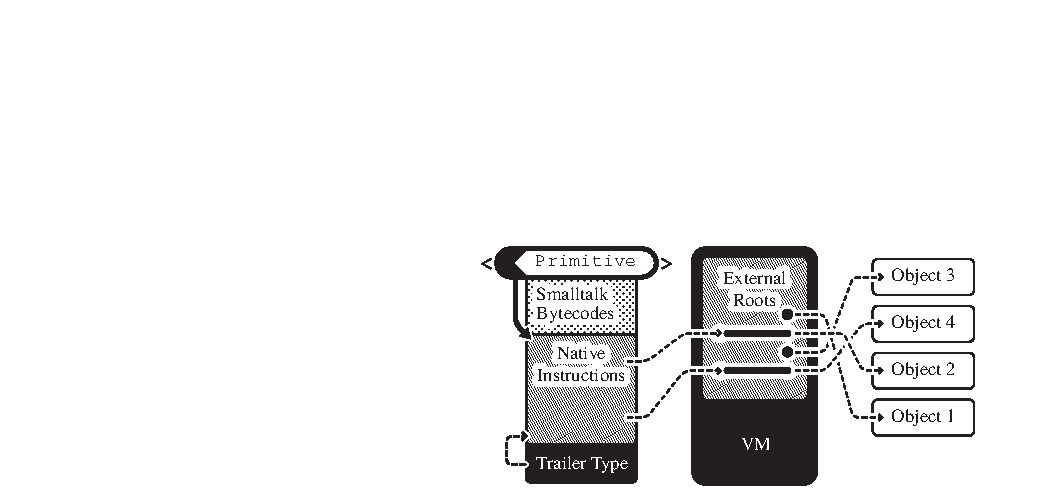
\includegraphics{externalRoots}
	\caption{Pointers in a CompiledMethod to objects registered as external roots are pinpointed at fixed offset in global VM-level object. \todo{possibly remove}
	}
	\figlabel{externalRoots}
\end{figure}

To deal with this problem the VM has a special array at a known address that contains pointers to high-level objects.
The garbage collector keeps this external roots array up to date.
Hence it is possible to statically refer to a Pharo object using a double indirection over the external roots.
Figure \figref{externalRoots} visualizes how native code directly accesses Pharo objects through this indirection.


% ===========================================================================
\subsection{Activating Native Code}

In this section we present the VM-level interaction of \NB.
Even though \NB handles most tasks directly at language-side it requires certain changes on VM level:
\begin{itemize}
	\item executable memory,
	\item activation primitives for native code.
\end{itemize}
%
Since \NB manages native code at language-side there is no special structure or memory region where native code is stored.
Native instructions are appended to compiled methods which reside on the heap.
Hence the heap has to be executable in order to jump to the native instructions.


% ---------------------------------------------------------------------------
\subsubsection{The \NB activation Primitive}
\seclabel{nbPrimitive}
% - show how code is generated in several pictures
%   1. no code => enter primitive and then primFailure fallback
%   2. running NB code generation
%   3. attach the native code to the compiled method
%   4. restart method and reenter primitive, this time running the native code
% - check for the VM identifier => mismatch triggers code regeneration

\todo{strip BENZO duplication: see how much overlaps, only put a small summary here and push detailed explanation to the benzo chapter}

In Section~\secref{generating} we explained how \NB creates FFI callouts at language-side.
However, so far we left out the part on how the generated native code is activated.

The examples in Section~\secref{nutshell}, especially Figure \figref{nativeBoostSyntax} show that each \NB FFI callout requires a special primitive.
Figure \figref{nativeCodeActivation} shows how a \NB method is activated.


\begin{figure}[h]
	\centering
	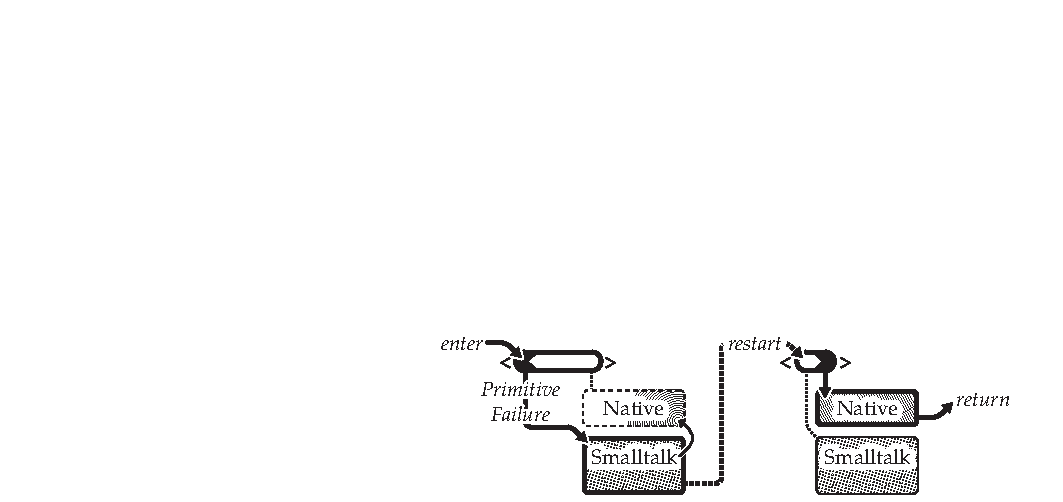
\includegraphics[scale=1.1]{nativeCodeActivation}
	\caption{Native code activation. The first call triggers the code generation. Then the method is restarted and the native code executed.}
	\figlabel{nativeCodeActivation}
\end{figure}

\begin{itemize}
\item In the first step (cf. \ding{182}) the \NB callout primitive is activated.
	The primitive checks if the compiled method actually contains native code.
\item On the first activation there is no native code available yet.
	Hence the primitive will fail and the Smalltalk body (cf. \ding{183}) of the \NB method gets evaluated.
	This is where \NB prepares the native code for the FFI callout.
\item After installing the native code in the method trailer, the \NB method is reactivated with the original arguments (cf. \ding{184}).
\item Again we end up in the \NB activation primitive (cf. \ding{185}).
	However, this time there is native code (cf. \ding{186}) available and thus the primitive jumps to the native code instead.
\end{itemize}

% ---------------------------------------------------------------------------
%\subsubsection{JIT Interaction}
% - explain drawback of VM primitive approach for NB when using a JIT
% - list overhead points (context switch, not able to jit)
% - show how COG solves this for certain other primitives

% ===========================================================================
%\section{Challenges}
%\seclabel{challenge}
% ===========================================================================

% - relocatable objects access overhead (almost never happens)
% - jit interaction (solved?)
% - callbacks
% - multi threaded code (diffcult..)
% - platform independence
%   - at the user-level of NBFFI not a problem
%   - plans to introduce abstract DSL for the low-level part of NB-FFI
%   - introducing variants of ASMJit to handle the last step (generating platform specific code)

% ===========================================================================
\section{Related Work}
\seclabel{relatedWork}
% ===========================================================================
\todo{only show FFI related work here! all the abstract implementations are covered in the Benzo secrtion}
% explain typical approaches (static and dynamic)

% - need to go into detail with ALIEN
% - C-FFI for Cog
% other less related approaches: Python ctypes ? SWIG ?

Typical Smalltalk system are isolated from the low-level world and provide only limited interoperability with C libraries.
However there are notable exceptions: Étoilé and Smalltalk/X.

Chisnall presents the Pragmatic Smalltalk Compiler \cite{Chis12a}, part of the Étoilé project, which focuses on close interaction with the C world.
The main goal of this work is to reuse existing libraries and thus reduce duplicated effort.
The author highlights the expressiveness of Smalltalk to support this goal.
In this Smalltalk implementation multiple languages can be mixed efficiently.
It is possible to mix Objective-C, Smalltalk code.
All these operations can be performed dynamically at runtime.
Unlike our approach, Étoilé aims at a complete new style of runtime environment without a VM. Compared to that, \NB is a very lightweight solution.


Other dynamic high-level languages such as Lua leverage FFI performance by using a close interaction with the JIT.
LuaJIT \cite{luaffi} for instance is an efficient Lua implementation that inlines FFI calls directly into the JIT compiled code.
Similar to \NB this allows one to minimize the constant overhead by generating custom-made native code.
The LuaJIT runtime is mainly written in C which has clearly different semantics than Lua itself.


On a more abstract level, high-level low-level programming \cite{Fram09a} encourage to use high-level languages for system programming.
Frampton et al. present a low-level framework  which is used as system interface for Jikes, an experimental Java VM.
%Additionally their framework is successfully used in MMTK \cite{Blac04a} which is used independently in several other projects.
%The \ttt{org.vmmagic} package is much more elaborate than \NB but it is tailored towards Java with static types.
However their approach focuses on a static solution.
Methods have to be annotated to use low-level functionality.
Additionally the strong separation between low-level code and runtime does not allow for reflective extensions of the runtime.
Finally, they do not support the execution and not even generation of custom assembly code on the fly.


QUICKTALK \cite{Ball86a} follows a similar approach as \NB.
However Ballard et al. focus mostly on the development of a complex compiler for a new \ST dialect.
Using type annotations QUICKTALK allows for statically typing methods.
By inlining methods and eliminating the bytecode dispatch overhead by generating native code QUICKTALK outperforms interpreted bytecode methods.
%The principal goals of QUICKTALK are performance improvements on dynamic typing.
Compared to Waterfall, QUICKTALK does not allow to leave the language-side environment and interact closely with the VM.


Kell and Irwin \cite{Kell11a} take a different look at interacting with external libraries.
They advocate a Python VM that allows for dynamically shared objects with external libraries.
It uses the low-level DWARF debugging information present in the external libraries to gather enough metadata to automatically generate FFIs.

% ===========================================================================
\section{Problems}
\seclabel{problems}
% ===========================================================================
% - most problems overlap with the problems mentioned in the Benzo chapter
% - address problems on a more high-level view


\subsection{Difficult Debug Cycles}
% - debugging facility (on a higher level than Benzo, see invisible VMs)
% 	- resolve C symbols
% 	- show C source code?


\subsection{Platform Independence}
% - general / direct dependence on assembler which is not good
% - low-level platform independence solved by Benzo (link to future reference to VirtualCPU)
% - platform independence on function level (see OSEnvironment as an Example)
% 	- requires explicit subclasses
% 	- manual maintenance + singletons
% - missing support for multi-platform code definition in a single method


\subsection{Limited Expressiveness}
% - fork example is hard to achieve (vm is not directly forkable)
% - current design makes it difficult to perform more C-like operations in one run
% - adopt benzo-level abstractions on VirtualCPU



% ===========================================================================
\section{Future Work}
\seclabel{futurework}
% ===========================================================================
Even though \NB shows good overall performance when it comes to callbacks it does not keep up with other \ST-based solutions.
In the current development phase not much attention was payed to callback performance as it is not a common use case for FFI callouts.
Fast callbacks require close interaction and specific modifications at VM-level.
However, initially \NB kept the modifications to the VM at a minimum.
We assume that we can reach the same performance as Alien relying on the same low-level implementation.

As a second issue we would like to address the callout overhead by using an already existing JIT integration of \NB.
Currently the VM has to leave from JIT-mode to standard interpretation mode when it activates an \NB method.
This context switch introduces an unnecessary overhead for an FFI callout.
A current prototype directly inlines the native code of a \NB method in the JIT.
Hence the cost for the context switch plus the cost of activating the \NB callout primitive can be avoided.
% \lf{This modification aims at better integrating \NB and the JIT such as it is done in LuaJIT.}



% ===========================================================================
\section{Conclusion}
\seclabel{conclusion}
% ===========================================================================
\todo{make proper summary}
In this paper we presented \NB a novel approach to foreign function interfaces.
Our approach relies only on a very generic extension of the VM to allow for language-side code to directly call native instructions.

Using a in depth evaluation of \NB comparing against two other \ST FFI implementations and LuaJIT we showed in Section~\secref{evaluation} that our language-side approach is competitive.
\NB reduces the callout overhead by more than a factor two compared to the two closest \ST solutions.

Compared to LuaJIT there is still space for improvements.
We measured a factor 30 lower calling overhead due to a close JIT integration.
However for typical FFI calls the absolute time difference between \NB and Lua is roughly $30\%$.
With a partial solution ready to integrate \NB closer with the JIT we expect to come close to Lua's performance.

Furthermore we showed that \NB essentially combines VM-level performance with language-side flexibility when it comes to marshal complex types.
New structures are defined practically at language-side and conversion optimizations are added transparently.

% =============================================================================
% empty version for the main document, where all the chapters are compiled together

\documentclass[a4paper,10pt,twoside]{../includes/ThesisStyle}
\usepackage[utf8]{inputenc}
\usepackage[T1]{fontenc}

\usepackage[left=1.5in,right=1.3in,top=1.1in,bottom=1.1in,includefoot,includehead,headheight=13.6pt]{geometry}\renewcommand{\baselinestretch}{1.05}


% =============================================================================
%\usepackage[sectionbib]{chapterbib}	% Cross-reference package (Natural BiB)
%\usepackage{bibunits}
%\usepackage{natbib}					% Put References at the end of each chapter
\usepackage{algorithm}
\usepackage{alltt}
\usepackage{amsfonts}
\usepackage{amsmath}
\usepackage{amssymb}
\usepackage{cite}
\usepackage{color}
\usepackage{enumerate}
\usepackage{fancyhdr}					% Fancy Header and Footer
\usepackage{graphicx}
\usepackage{ifthen}
\usepackage{latexsym}
\usepackage{multirow}
\usepackage{rotating}					% Sideways of figures & tables
\usepackage{stmaryrd}
\usepackage{subfigure}
\usepackage{url}         
\usepackage{xspace}

\usepackage[a4paper,pagebackref,hyperindex=true]{hyperref}
        

% =============================================================================

% Table of contents for each chapter
\usepackage[nottoc, notlof, notlot]{tocbibind}
\usepackage{minitoc}
\setcounter{minitocdepth}{1}
\mtcindent=15pt

\setcounter{secnumdepth}{3}
\setcounter{tocdepth}{2}
  
% =============================================================================
% Fancy Header Style Options

\pagestyle{fancy}                       % Sets fancy header and footer
\fancyfoot{}                            % Delete current footer settings

%\renewcommand{\chaptermark}[1]{         % Lower Case Chapter marker style
%  \markboth{\chaptername\ \thechapter.\ #1}}{}} %

%\renewcommand{\sectionmark}[1]{         % Lower case Section marker style
%  \markright{\thesection.\ #1}}         %

\fancyhead[LE,RO]{\bfseries\thepage}    % Page number (boldface) in left on even
% pages and right on odd pages
\fancyhead[RE]{\bfseries\nouppercase{\leftmark}}      % Chapter in the right on even pages
\fancyhead[LO]{\bfseries\nouppercase{\rightmark}}     % Section in the left on odd pages

\let\headruleORIG\headrule
\renewcommand{\headrule}{\color{black} \headruleORIG}
\renewcommand{\headrulewidth}{1.0pt}
\usepackage{colortbl}
\arrayrulecolor{black}

\fancypagestyle{plain}{
  \fancyhead{}
  \fancyfoot{}
  \renewcommand{\headrulewidth}{0pt}
}


% =============================================================================
% Clear Header Style on the Last Empty Odd pages
\makeatletter

\def\cleardoublepage{\clearpage\if@twoside \ifodd\c@page\else%
  \hbox{}%
  \thispagestyle{empty}%              % Empty header styles
  \newpage%
  \if@twocolumn\hbox{}\newpage\fi\fi\fi}

\makeatother

\newenvironment{maxime}[1]
{
\vspace*{0cm}
\hfill
\begin{minipage}{0.5\textwidth}%
%\rule[0.5ex]{\textwidth}{0.1mm}\\%
\hrulefill $\:$ {\bf #1}\\
%\vspace*{-0.25cm}
\it 
}%
{%

\hrulefill
\vspace*{0.5cm}%
\end{minipage}
}

\let\minitocORIG\minitoc
\renewcommand{\minitoc}{\minitocORIG \vspace{1.5em}}


\renewcommand{\epsilon}{\varepsilon}

% centered page environment
\newenvironment{vcenterpage}
	{\newpage\vspace*{\fill}\thispagestyle{empty}\renewcommand{\headrulewidth}{0pt}}
	{\vspace*{\fill}}
	
	
% =============================================================================
\newboolean{showcomments}
\setboolean{showcomments}{true}

\ifthenelse{\boolean{showcomments}} {
	\newcommand{\ugh}[1] {\textcolor{red}{\uwave{#1}}}	% please rephrase
	\newcommand{\ins}[1] {\textcolor{blue}{\uline{#1}}}	% please insert
	\newcommand{\del}[1] {\textcolor{red}{\sout{#1}}}	% please delete
	\newcommand{\chg}[2] {								% please change
		\textcolor{red}{\sout{#1}}{\ra}
		\textcolor{blue}{\uline{#2}}}
	\newcommand{\nbc}[3]{								% comment
		{\colorbox{#3}{\bfseries\sffamily\scriptsize\textcolor{white}{#1}}}
		{\textcolor{#3}{\sf\small$\blacktriangleright$\textit{#2}$\blacktriangleleft$}}}

}{
	\newcommand{\ugh}[1]{#1}							% please rephrase
	\newcommand{\ins}[1]{#1}							% please insert
	\newcommand{\del}[1]{}								% please delete
	\newcommand{\chg}[2]{#2}							% please change
	\newcommand{\nbc}[3]{}								% comment
}

% =============================================================================
\usepackage[a4paper,pagebackref,hyperindex=true]{hyperref}


% Links in pdf
\usepackage{color}
\definecolor{linkcol}{rgb}{0.0, 0.0, 0.0} 
\definecolor{citecol}{rgb}{0.0, 0.0, 0.0} 

% Change this to change the informations included in the pdf file
% See hyperref documentation for information on those parameters
\hypersetup {
	bookmarksopen=true,
	pdftitle="Design and Use of Anatomical Atlases for Radiotherapy",
	pdfauthor="Olivier COMMOWICK", 
	pdfsubject="Creation of atlases and atlas based segmentation", %subject of the document
	%pdftoolbar=false, % toolbar hidden
	pdfmenubar=true, %menubar shown
	pdfhighlight=/O, %effect of clicking on a link
	colorlinks=true,
	pdfpagemode=None,
	pdfpagelayout=SinglePage,
	pdffitwindow=true,
	linkcolor=linkcol,
	citecolor=citecol,
	urlcolor=linkcol
}

% =============================================================================
\newcommand{\figlabel}[1]{\label{fig:#1}}
\newcommand{\seclabel}[1]{\label{sec:#1}}
\newcommand{\tablabel}[1]{\label{tab:#1}}

\newcommand{\figref}[1]{Figure~\ref{fig:#1}}
\newcommand{\secref}[1]{Section~\ref{sec:#1}}
\newcommand{\tabref}[1]{Table~\ref{tab:#1}}

\newcommand{\commented}[1]{}

\newcommand{\eg}{\emph{e.g.,}\xspace}
\newcommand{\ie}{\emph{i.e.,}\xspace}


\newcommand\fix[1]{\nb{FIX}{#1}}
\newcommand\todo[1]{\nb{TO DO}{#1}}

% =============================================================================

\graphicspath{{.}{../figures/}}

\begin{document}
% ===========================================================================

\chapter{\B Prototype Application Validation}
\chaplabel{validation}
\minitoc
% ===========================================================================
\introduction
% ===========================================================================

In \chapref{ffi} we presented \NB, a mature language-side \FFI implementation that makes heavy use of \B's infrastructure.
\NB is only one of three applications that are based on \B that were initially outlined in \secref{benzo-usecase}.
While \NB is considered stable, the two other applications are currently only prototypes: dynamic primitives and a language-side \JIT.
Hence we will present the two solutions combined in this chapter.

As first we will present \WF, dynamic primitives based on \B.
\WF takes advantage of the metacircular approach of \PH's \VM and makes the primitive definition available at runtime.
This is a step forward from the typical metacircular approach where the whole reflective power of the host environment can only be used at compile-time.
Once the \VM is compiled, all the high-level definitions that existed at compilation time are no longer accessible from language-side.
\WF tries to make a fraction of the original compile-time definitions accessible.

\todo{probably retrofit to the final results of \NBJ}\enlargethispage{\baselineskip}
The second prototype, \NB a language-side \JIT compiler takes the core idea of \WF even further.
\WF is capable of defining new primitives at runtime which are not reentrant: it is not possible to activate \PH methods from within primitives.
However, this is what happens in jitted methods: it is possible to switch seamlessly between native methods and standard \PH methods using bytecode evaluation.
Much like the primitives, the \JIT can not be changed from language-side and this is where we bring \NBJ into play.
\NBJ reimplements the \VM-level \JIT compiler at language-side and uses \B to install the native code.


% ===========================================================================
%\newpage
\section{\WF: Dynamic Primitives}
\seclabel{val-waterfall}
% ===========================================================================

\begin{figure}[h]
	\centering
	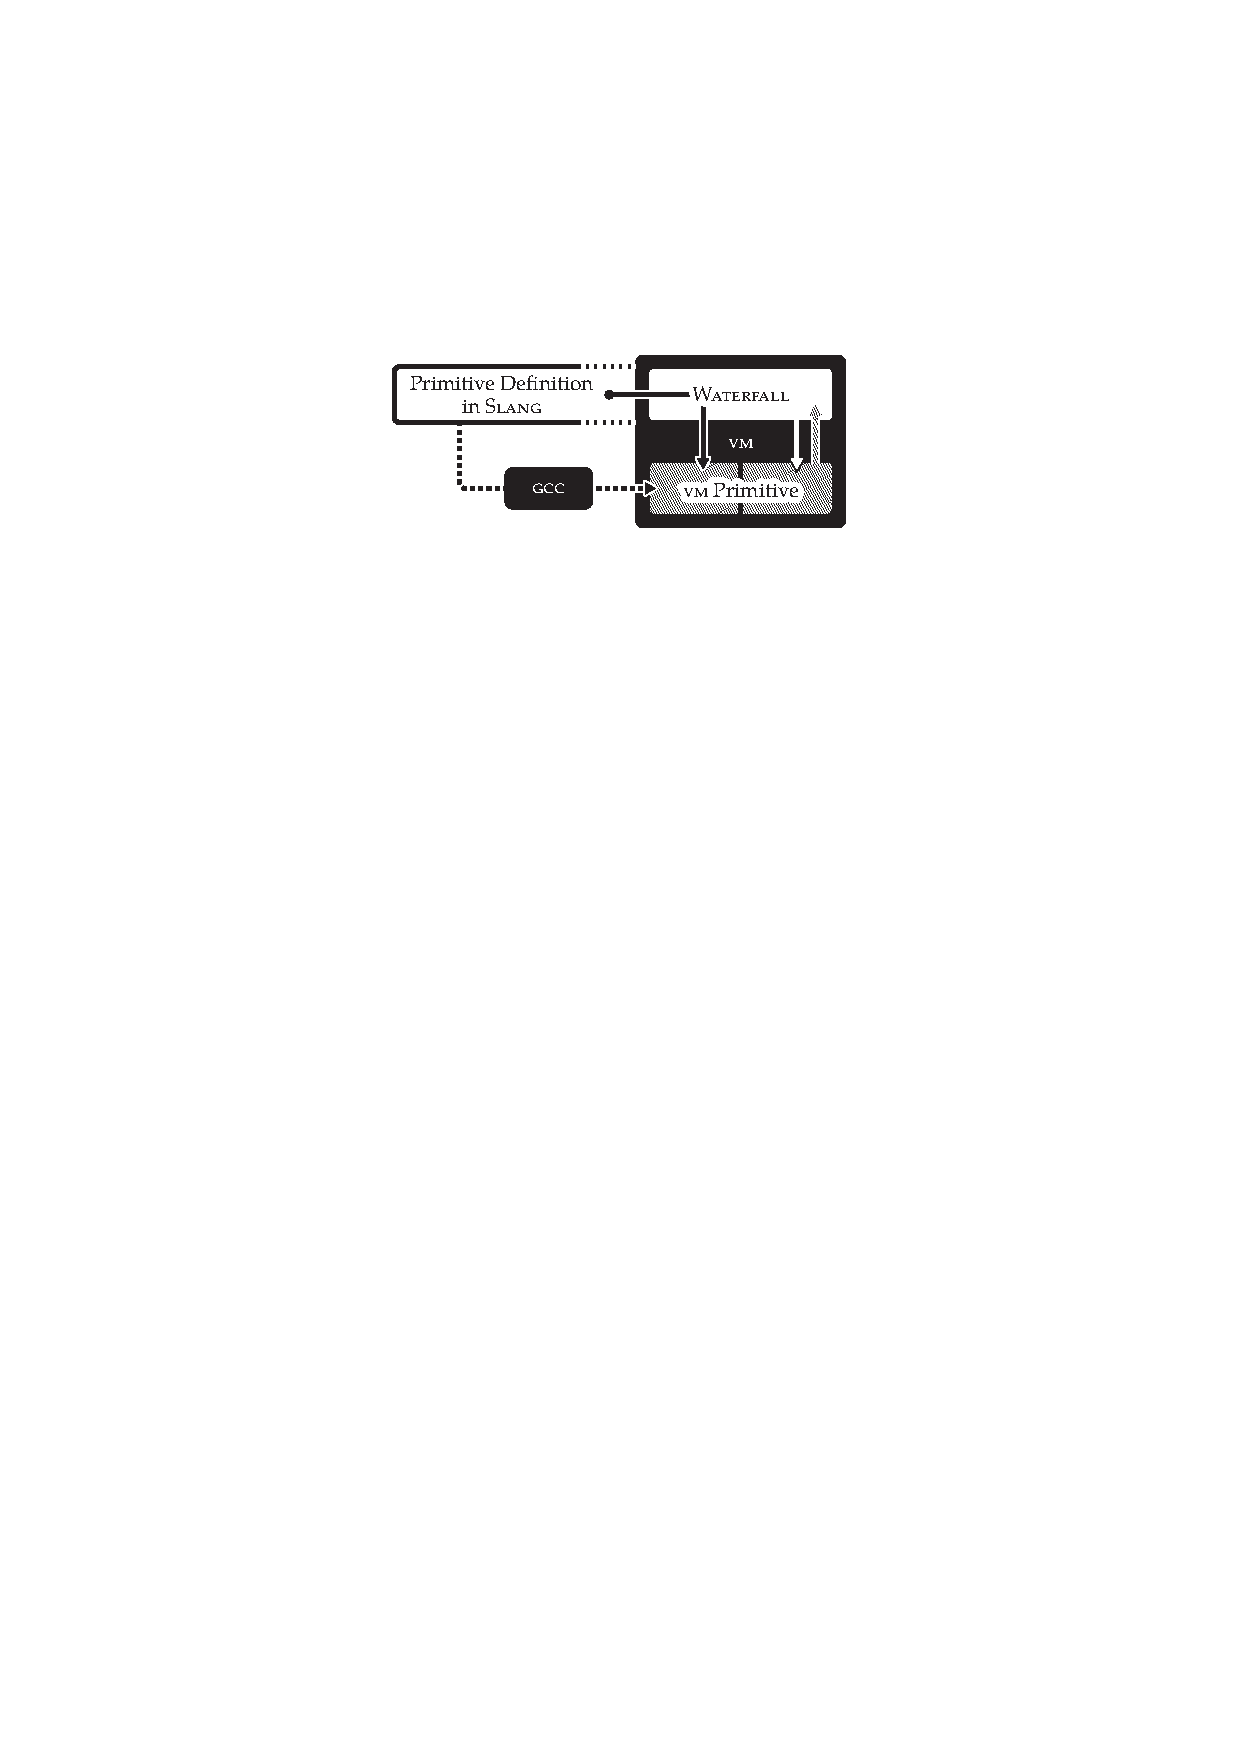
\includegraphics[scale=\imagescale]{waterfall-overview}
	\caption{\WF Overview}
	\figlabel{val-waterfall-overview}
\end{figure}

\noindent In this section we present \WF, a compiler toolchain that allows primitives to be changed dynamically from language-side.
We successfully use \WF to change and recompile whole \VM plugins such as the file plugin as we show in the following \secref{val-waterfall-plugins}.

% -----------------------------------------------------------------------------
\subsection{Background}
\seclabel{val-waterfall-background}
% -----------------------------------------------------------------------------

\WF is our second application on top of \B after \NB, the complete \FFI library previously presented in \chapref{ffi}.
\NB uses \B to generate the glue code between \PH and the external library.
Even though \NB is extendable it is not used to directly synthesize new functionality, the main functionality is defined the external libraries typically written in a low-level language such as C.
Interestingly, the \NB methods containing the callouts behave almost like the existing primitive methods of \PH.
These primitives define a hook into \VM-level native functionality.
In \PH the same mechanism is also used to activate plugins which are again similar to an \FFI callout from language-side.
However, primitives and plugins are statically defined and modifications happen outside \PH.
This is where the domain of \WF begins.

\WF provides infrastructure to dynamically compile and install primitives on top of the \B infrastructure at language-side in \PH.
As we will describe in more detail in the following sections, the \PH \VM is written in a metacircular fashion.
Hence the definition of plugins and primitives can be loaded in standard \PH.
Typically this happens only at compile-time of the \VM, where these definitions are exported to C and compiled to the \VM binary.
Once compiled, the original high-level description of primitives and plugins is no longer accessible from \PH.
As a consequence, existing primitives or plugins can not be changed at runtime.

\WF brings the static primitive definitions to live again.
Just loading the original definitions in \PH does not bring them back to live, even though we can now inspect the definition and browse the sources.
\WF compiles these definitions to native code and installs them with \B as new primitives.
With this infrastructure primitive and plugin modifications are not limited to \VM compilation time.

\paragraph{A Metacircular \VM Written in \Slang}

\WF is implemented in \PH which uses the \urlfootnote{\Cog \VM}{http://www.mirandabanda.org/cogblog/}, originating from the \Squeak \VM\cite{Inga97a}.
The \VM itself is written in a dialect of \ST called \Slang that is essentially limited to the functionality that can be expressed with standard C code.
\Slang serves for two purposes: a high-level C preprocessor, a interactive simulator of the \VM.
The first point has severe consequences.
\Slang basically has the same syntax as \ST but is semantically constrained to expressions that can be resolved statically at compilation or code generation time and are compatible with C.
Hence \Slang's semantics are closer to C than to \ST.
This fact is also visible in the simulator for the \VM.
If \Slang were \ST, separate parts of the \VM could be directly evaluated.
However, since \Slang is bound to C expressions, the simulator sets up a byte array as memory.
The simulated \VM then accesses this byte array as if it were the native memory.

In conclusion we see that the \PH \VM has an abstract representation of the \VM available for simulation.
This abstract representation is then used to generate C sources, already lowering the abstraction level.
After compiling the C sources the original representation of the \VM is not directly accessible anymore.
For instance, even debug symbols are usually stripped from the final binary for performance reasons.
Of course this implies that the \VM can not be changed nor directly inspected from language-side.


\paragraph{Primitives in \PH}
\PH is a highly reflective environment where classes and methods can be changed at runtime, even the current execution context is accessible.
For instance this is used to implement an exception mechanism purely at language-side in \PH.
However, some features can not be implemented at language-side.
\PH uses primitive methods, that instead of evaluating \PH-code switch to a \VM routine.
As already partially explained in \secref{benzo-vm-interaction}, whenever a method is compiled with the \ttt{primitive} pragma as shown a flag is set on the \ttt{CompiledMethod}. 
If the \VM tries to activate such a method, instead of interpreting the bytecodes it calls the corresponding function at \VM-level~\cite{Gold83a}.
We distinguish three categories of primitives based on their functionality: certain parts of the language semantics, \OS-level functionality that can not be implemented in \PH itself and a third less important category where performance is critical.

As we mentioned in the previous paragraph, these primitives are bound to the \VM and can not be changed at runtime.
However, for a certain subset of these primitives we can write language-side substitutes in pure \PH-code.
These primitives are called non-essential and are mainly used for optimization purposes. 
In contrast there are essential primitives which are for instance used during start up of the \PH environment.
Two prominent examples of essential primitives are the ones used for creating new objects or activating a block.

\paragraph{Instrumenting Primitives}
In the context of \WF we are interested in which parts of the system we can modify and thus we draw our attention to these essential primitives.
The only way to modify these primitives is by creating wrappers but that brings a new problem.
Imagine that we wrap around the primitive which creates a new object.
What happens now if the additional wrapper code needs a new object?
It will call the very same primitive that we just wrapped, without protection this causes infinite recursion.
Since technically the wrapper code should live at a different abstraction level than the original primitive we have find our selves mixing meta-levels.

The most radical approach to avoid this meta-recursion is to change the primitive externally.
In the case of \PH this means changing the \Slang sources, exporting and compiling the primitive and restarting the \PH environment on top of this changed \VM.
However, this approach stands in contrast to the reflective nature of \PH where most functionality can be changed at runtime.
Also it is not always suitable to restart the \PH process to modify a small part of the system.

%----------------------------------------------------------------------------
\subsection{\WF's Contribution}
Following the implementation overview of the \PH \VM and the differentiation of different primitives we identify two main benefits of changing \VM primitives at runtime with \WF:

\begin{enumerate}
	\item Reducing \VM complexity by implementing non-essential primitives reflectively at language-side.
	\item Dynamic instrumentation of primitives.
\end{enumerate}

\paragraph{Reducing \VM Complexity}
Low-level \VM extensions are only justified in the presence of strong performance requirements (see \secref{benzo-related}).
All non-essential primitives fall into this category since these primitives can be implemented in \PH without restrictions.
However, in certain cases for performance a language-side implementation is unsuitable.
Additionally we already know that these primitives are available as \Slang code at \VM generation time.
Using \WF, these primitives can be implemented at language-side based on the unmodified \Slang sources.
This means that these primitives become first-class citizens of the high-level environment and thus evolve with less effort.
Thus, \WF opens new possibilities of changing \PH that were previously possible only with significant overhead.

\paragraph{Essential Primitives}
For essential primitives the previous argument does not hold since a static version is needed for a correct startup of the system.
These primitives can not be directly replaced by a language-side implementation using \WF.
Even though \WF itself avoids meta-recursion by generating low-level code with \B.
However, \B itself relies on essential primitives as it is written in \PH.
This imposes certain restrictions how and when these essential primitives can be modified with \WF during system startup.
These restrictions are more related to the underlying \B infrastructure than \WF.
For instance already exposed similar limitations with the \B-based \FFI when used during startup (see \secref{ffi-startup-recursion}).
Nevertheless, nothing prevents from replacing essential primitives at runtime with customized versions, once the system startup is completed. 

\paragraph{Extended Primitive Instrumentation}
Instrumentation of essential primitives from lan\-guage-side is an error-prone task falling in many cases in non-termination due to previously described meta-recursion. 
An example of this behavior, can be observed when changing the essential \ttt{basicNew} primitive, which is responsible for instantiating new objects.
Only very limited instrumentation is possible at language-side, for instance counting how many instances have been created.
This only works since the \VM internally does not represent small integers as full objects.
However, this is only true up to some extent.
Small integers bigger than $2^{30}$ are transformed to a more expensive object representation since they no longer fit in a machine word of the 32-bit \VM. 
These big integers will use the \ttt{basicNew} primitive again as they are not implement in the \VM but in at language-side.
Thus, we are back the original problem of running into meta-recursion.
So even this very simple example has unwanted side-effects that are not directly visible.
More complex instructions tasks will inevitably suffer from the same problems.

Using reflective techniques it is possible to escape from this meta-recursion, however, with a considerable overhead.
\WF avoids these issues since the instrumentation code for primitives will be implemented at the lowest level on top of \B.
In \secref{val-waterfall-performance} we show how \WF, the \B based approach for generating primitives on the fly, outperforms the reflective solutions for primitives instrumentation. 


% -----------------------------------------------------------------------------
\subsection{\WF Implementation}
\seclabel{val-waterfall-implementation}
% -----------------------------------------------------------------------------
\WF uses \B's mechanism for replacing primitive methods with customized versions that are nativized dynamically as described in \chapref{benzo}.
The loophole described there is exploited by \WF to enable dynamic modification of \VM behavior and hence bring primitives to life at language-side.
From a high-level point of view \WF provides two services which work transparently: 

\begin{enumerate}
	\item Compilation of \Slang code on demand (lazily).
	\item A clear interface for executing, at runtime and from language-side, the native code generated.
\end{enumerate}

\noindent The first item allows to change the code of primitives at language-side and generate the corresponding native code when needed. 
It also provides the possibility to write methods or functionality with the same \ST syntax but with a static semantic. 
It consists essentially of a transformation toolchain that transforms the \Slang sources to native code using a \B-based compilation toolchain.

The second item enables the execution of the dynamically generated native code.
This includes for instance the finding of addresses of \VM internal symbols and all the effort to link the two worlds, \ST and native.
\WF relies on \B for most of this low-level functionality.
In particular \NB, the \B-based \FFI presented in \chapref{ffi}, is used for interfacing with C libraries (\ttt{dlsym}). 

% -----------------------------------------------------------------------------
\paragraph{Architecture Overview}
The \WF infrastructure is mainly divided in the following two parts: 
\begin{itemize}[nolistsep,noitemsep]
	\item the installed \Slang sources,
	\item a \B-based compilation toolchain.
\end{itemize}
The \WF compiler transforms the \Slang sources to native code through various transformation steps as show in \figref{waterfall-architecture}.
In order to work properly \WF needs the complete \Slang sources for compilation unit (primitive or plugin) to be loaded upfront.
Once loaded in the \PH image the \AST of the \Slang sources are available which form the input for the \WF compiler.
This means that it is possible to write custom plugins in \PH and transform them using \WF as long as the written \PH code uses the restricted \Slang subset.
As mentioned earlier, the major difference to normal \PH code is the lack of real polymorphism since \Slang is more like C with a \ST syntax.

Technically the \WF compiler takes over the part of the \Slang to C converter and of \GCC in the normal \VM compilation process.
\WF, much like the \Slang to C converter, has to take care of certain type information present in the \Slang sources.
For instance we extract from the type information if arguments are used by value or reference.
With this information we generate native code using a simple stack based strategy for temporary variables.
As for the part of \GCC, \WF in its current state is of course far less complex and the resulting the native code is inferior to \GCC's optimized output.
To simplify the prototype \WF only uses a simple stack strategy instead of register allocation for temporaries.
Additionally \WF does not use intermediate representations (\IR) such as static single assignment (\SSA) to perform elaborate optimizations \cite[Ch.\ 1]{Appe98a}.


% -----------------------------------------------------------------------------
\paragraph{Compilation Steps}
As shown in \figref{waterfall-architecture} the \WF compiler transforms the \AST of the \Slang input to \PH primitives.

\begin{figure}[h]
	\centering
	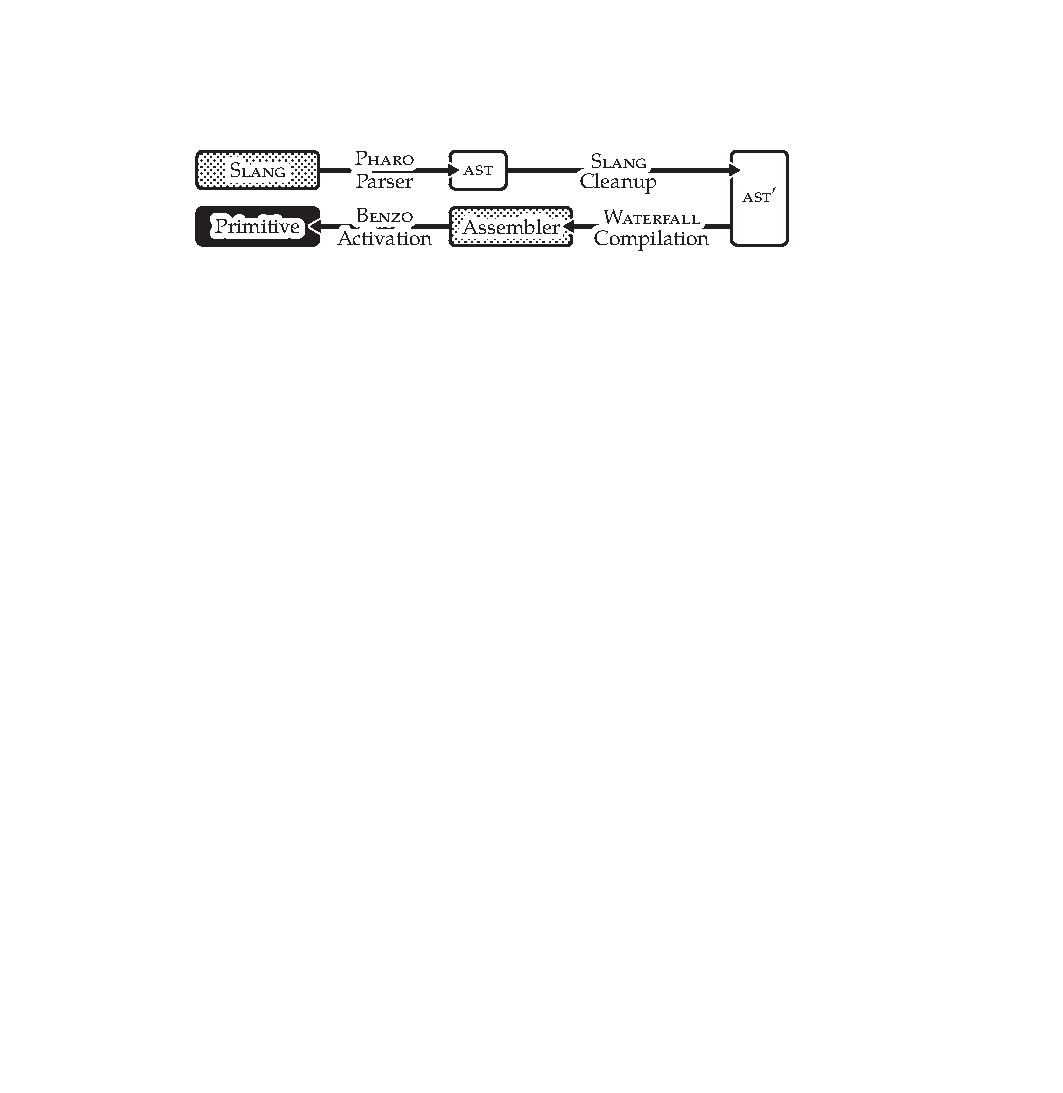
\includegraphics[scale=\imagescale]{waterfall-architecture}
	\caption{\WF Compilation Steps}
	\figlabel{waterfall-architecture}
\end{figure}

\noindent We divide the \WF compiler into four distinct steps:
\begin{description}
\item[\Slang to \AST:] The first step is to access the \AST of the \Slang source method which happens automatically by loading the \Slang code in the \PH image.
At this stage \WF also recursively collects the set of reachable \Slang methods.


\item[\AST Purification:] In a second step certain expressions of the original \Slang \AST are transformed into custom \WF expressions that can be easier transformed later on.
For instance \WF converts C macros that are supported in \Slang which of course only make sense when using a standard C compiler.

\item[\AST to \ASM:] The real native compilation happens in the third step where an \AST-visitor creates assembler instructions using \B's \AsmJIT.
At this point external symbols are statically resolved and directly inlined in the final \ASM code.

\item[\ASM to Primitive] Although not strictly part of the compilation, in the fourth step the final native instructions are installed as a primitive methods using \B (see \secref{benzo-benzo} for more details).
\end{description}


% -----------------------------------------------------------------------------
\paragraph{Dynamically Replacing Primitives}
After explaining the general architecture and the different compilation steps of \WF we shed some light on how the primitives are actually installed.
In reality we rely 100\% on \B for this feature.
Once the native code is generated we transform the target method to a special \B-enabled method that contains the native code.
This procedure is explained in detail in \secref{benzo-benzo} where we show the implementation details of \B.

From a user point-of-view we only have to make sure that the corresponding \Slang sources are available and then hand over that source method to \WF to compile and install it.
Once the installation is complete, the resulting \B-enabled method will contain behave like a \Slang primitive compiled with the original approach using \GCC.

% -----------------------------------------------------------------------------
\paragraph{Dynamically Replacing Plugins}
In \PH there is no real distinction between primitives and plugins as we illustrate with the following code snippets.
The first one depicts an essential primitive to allocate new objects.
The second code example shows the a plugin primitive to open a new file stream.
%
\begin{stcode}[
	caption={\ttt{Object>>\#basicNew} Primitive},
	label={lst:validation-basicnew}]{3}
basicNew
  <primitive: 70>
  OutOfMemory signal.
\end{stcode}
%
\begin{stcode}[caption={\ttt{FilePlugin>>\#open:writeable:} Plugin Primitive}]{5}
open: pathString writable: writableFlag
  "Open a file at the given pathString, and return
   the file ID obtained."
  <primitive: 'primitiveFileOpen' module: 'FilePlugin'>
  ^ nil
\end{stcode}
%
The main difference between primitives and plugins is only how they are distributed.
Primitives are inlined in the \VM and can not be loaded at runtime, while plugins can be loaded dynamically and are bundled separately.
That also means that there is no difference in handling plugins for \WF, the compilation and installation process is exactly the same.

% -----------------------------------------------------------------------------
\subsection{\WF Validation}
\seclabel{val-waterfall-performance}
% -----------------------------------------------------------------------------
After explaining the implementation details of \WF we would like to present a thorough evaluation of the \WF infrastructure.
We split up the validation in two parts following the outlined applications of \WF in the introduction.
The first part describes the performance of \WF when used for instrumenting primitives.
This is the major field of application for \WF as it stresses its dynamic nature.
In contrast to that we evaluate the performance of a \WF compiled plugin in the second part of the validation.
Evaluating a whole plugin puts more stress on the quality of the generated code than the fact that we can dynamically modify primitives.
A more detailed analysis of \WF is also available separately \cite{Char13a}.


% -----------------------------------------------------------------------------
\subsubsection*{Validation of Dynamic Primitives}

In this first part of the \WF validation we compare the performance of \WF generated primitives in \PH.
In the first part we simply measure the speed of a dynamically replaced primitive, while in the second we add instrumentation overhead.
For the simple replacement we choose the simple integer operation "greater than" (\ttt{$>$}) and for instrumentation the more complex \ttt{basicNew} primitive.

\paragraph{Simple Dynamic Primitives}
In this first validation we compare the speed of the \WF generated code on a simple "greater than" primitive.
The primitive is rather simple as it only works on small integers arguments and delegates the functionality for other types to its superclass.
The code for the \ttt{Smallinteger} operation looks as follows.
%
\begin{stcode}{3}
> aNumber
	<primitive: 4>
	^super > aNumber
\end{stcode}
%
The fallback code at the end of the method triggers a slower "greater than" implementation on the super class \ttt{Integer} which mostly deals with the multitude of possible arguments to \ttt{>}.

\begin{stcode}{1}
> aNumber
	aNumber isInteger 
		ifFalse:[
			^ aNumber 
				adaptToInteger: self andCompare: #> ]
	self negative == aNumber negative
		ifFalse: [ ^ aNumber negative ].
	self negative
		ifTrue: [ ^(self digitCompare: aNumber) < 0 ]
		ifFalse: [ ^(self digitCompare: aNumber) > 0 ].
\end{stcode}


\noindent For comparing performance of the "greater than" primitive we use three different approaches:
\begin{enumerate}[noitemsep,nolistsep]
	\item the standard primitive provided by the \VM,
	\item the fallback language-side implementation that is triggered whenever the standard primitive failed,
	\item the reimplementation with \WF (not instrumented).
\end{enumerate}
%
We run the three approaches by measuring the cumulative time over one million primitive activations averaged over $100$ runs.
The absolute numbers are less important than the relative factor between them.
We present the results of this experiment in ~\tabref{val-waterfall-performance}.
%
\begin{table}[H]
    \centering
    \begin{tabular}{rSS}
					& {Running Time [ms]} & {Relative Time} \\\midrule
		Unmodified	&   6.4(14)           & 1.0\\
		Fallback	& 195.0(16)           & \approx30.0 \\
		\WF	        &  22.8(17)           & \approx3.6
    \end{tabular}
    \caption[\WF Speed Comparison: Large Integer]{Comparing running time of different implementations of integer arithmetic primitive.}
    \tablabel{val-waterfall-performance}
\end{table}

\noindent As expected \WF's solution outperforms pure reflective one by factor $9$ to $10$.
\WF clearly outperforms a purely reflective solution since all the meta programming overhead for the intercession mechanism is avoided.
This results thus makes a whole new set of runtime extensions feasible that were previously limited by their strong performance penalty.
Furthermore the performance penalty over a completely optimized \VM solution that has extreme optimization techniques, such as inlining and register allocation, is less than a factor of $4$.

\paragraph{Essential Primitive Instrumentation}
As a second validation target for primitives we chose to instrument \ttt{basicNew} which is a critical primitive for object allocation.
Like the previous "greater than" primitive this belongs to the set of essential primitives that are used during startup of the image.
For instrumentation \ttt{basicNew} is again a rather tricky target as wrong code easily leads to infinite recursion.
However, this can be avoided with a rather costly recursion guard.
We chose a rather simple instrumentation method by simply printing the address of the allocated object to the standard output stream.
We validate the four flavors of the \ttt{basicNew} primitive:
\begin{enumerate}[noitemsep,nolistsep]
	\item the unmodified primitive,
	\item a reflectively instrumented primitive with a recursion guard written in \PH,
	\item a \WF generated and instrumented version,
	\item a \WF generated version without instrumentation.
\end{enumerate}

\noindent We measure again with the same setup as for the previous validation of the "greater than" primitive.
The outcome of this validation is shown in \tabref{val-waterfall-basicnew}.
%
\begin{table*}[h]
    \centering
    \begin{tabular}{rSS}
					                      & {Time [ms]} & {Relative Time} \\\midrule
        Unmodified                        &  0.28(16)           &          1 \\
        Secure reflective instrumentation & 27.72(40)           & \approx 99 \\
        \WF-based instrumentation         &  7.72(27)           & \approx 28 \\
        \WF-based non-instrumentation     &  7.08(23)           & \approx 25 \\
    \end{tabular}
    \caption[\WF Speed Comparison: \ttt{basicNew}]{Slowdown comparison for instrumentation of the  essential primitive \ttt{basicNew}.}
    \tablabel{val-waterfall-basicnew}
\end{table*}
%
Again the results present a similar picture as for the "greater than" validation.
However, since we added instrumentation this time, the reflective \PH is significantly slower than the unmodified version of the primitive.
This proves our theory that in certain performance critical cases reflective solutions are not sufficient.
While we were able to circumvent the recursion problem rather elegantly, the recursion guard is simply too slow to be used by default.
Compared to that, the \WF-based instrumentation is a factor $3$ faster than the reflective solution.
We see that the instrumentation overhead compared to the non-instrumented \WF version is in the range of only $0.7$ms whereas in the \PH version the overhead is several magnitudes higher.
Unlike for the simpler "greater than" primitive \WF is slower: factor $25$ instead of only a factor $3.6$ previously.
This shows that there is certainly room for performance improvements for \WF.

% -----------------------------------------------------------------------------
\subsubsection*{Validation of Dynamic Plugins}
\seclabel{val-waterfall-plugins}

In this second part of the \WF performance evaluation we focus on whole plugins.
Even so we already mentioned that from a language-side point of view there is no difference in plugins and primitives there typically is a significant difference in code size.
While primitives tend to be small and do simple tasks very efficiently (like arithmetic operations) plugins follow a different approach where larger more complex tasks are solved externally.
 
\paragraph{\WF Compiled File Plugin}
\paragraph{\WF Compiled ??? Plugin}
\todo{Write about the File Plugin Validation}\\
\todo{Possibly Validate other plugin}


% -----------------------------------------------------------------------------
\subsection{Problems and Outlook}
% -----------------------------------------------------------------------------

\WF is still a research prototype and thus there are several issues that problems that require attention with the most obvious one being performance.
We have shown that \WF is fast enough to compete against dynamic primitive instrumentation written at language-side, but when compared to native solutions we are still up to two magnitudes slower.
For simplicity \WF currently does not apply any optimizations which still leaves room for improvements.
For instance we do not apply register allocation yet.
However, in our eyes it does not make sense to implement a specific register allocator for \WF itself.
Instead, we envision to use a future platform independent intermediate representation of \B that we presented in \secref{benzo-problems-platform-independence}.
This way most optimizations only require one implementation from which all \B applications benefit.
Using this new \IR would have very little impact on the current \WF compiler infrastructure as we would only have to replace the \AST to \ASM compilation step.
Instead of generating the \ASM we use the \B \IR and let \B generate the native code for the primitives.

\WF is currently only a research prototype that is not used in production.
Also we have seen that there is a significant overlap with the \NB \FFI.
For example, many plugins wrap around existing external libraries and thus are perfect candidates for \NB.
Even though \WF would add a lot of flexibility for such plugins, we believe that \NB is more intention revealing and less confusing that dealing with the semantic differences of \Slang code over \PH code.
Nevertheless, this still leaves the big field of instrumentation open for \WF.
Additionally, for documentation purposes it makes sense to load the \Slang definition of all the essential primitives into the \PH image.
In this case \WF would be a perfect way to bring these primitives to live for exploration purposes.

\todo{better \JIT interaction (leading to the following \NBJ section)}

% ===========================================================================
\newpage
\section{\NBJ: Language-side \JIT Prototype}
\seclabel{val-nabujito}
% ===========================================================================

\begin{figure}[h]
	\centering
	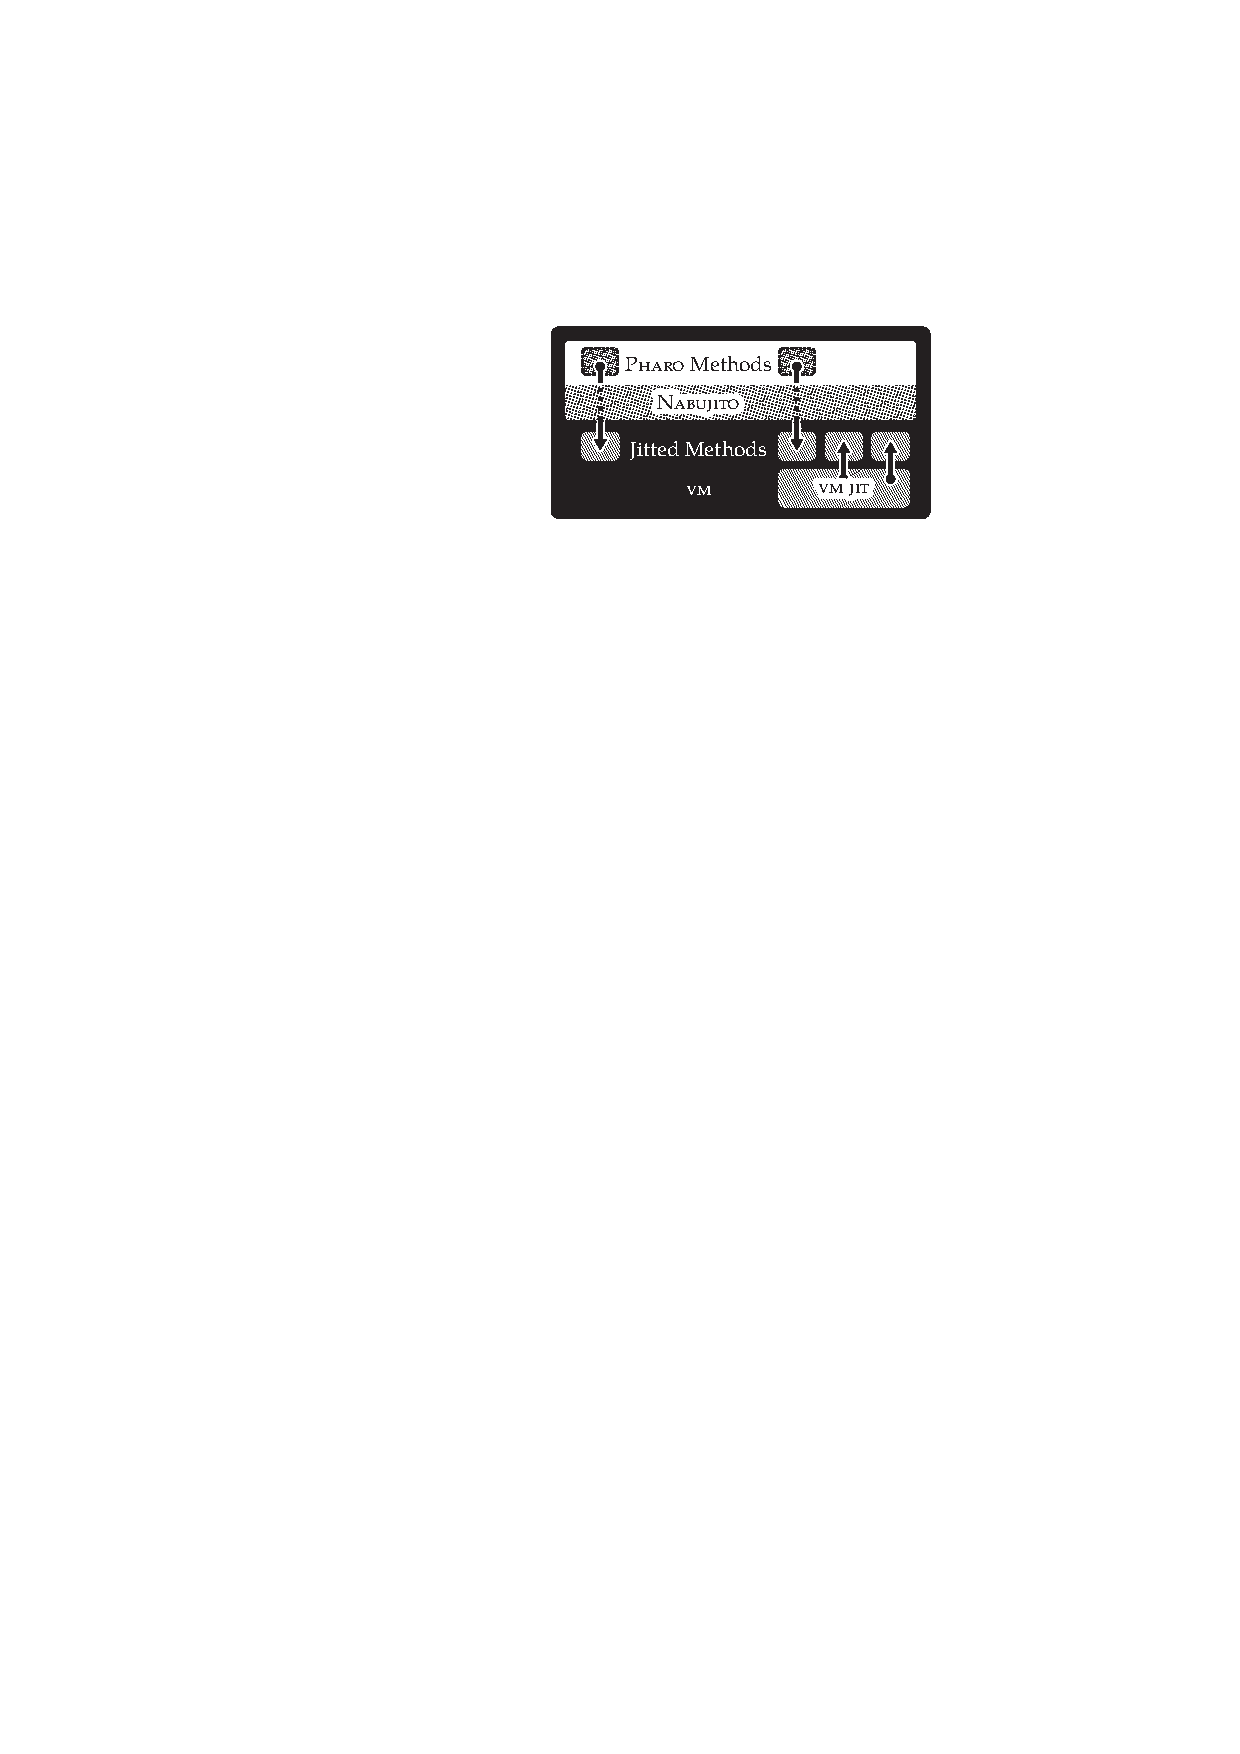
\includegraphics[scale=\imagescale]{nabujito-overview}
\end{figure}

\noindent In this section we present \NBJ, a \B-based approach for a language-side \JIT compiler.
\todo{Introduction}

% ---------------------------------------------------------------------------
\subsection{Background}
\seclabel{val-nabujito-background}
% ---------------------------------------------------------------------------

\NBJ goes even further than \WF using almost the same techniques.
However, instead of focusing on primitives, \NBJ generates native executable code for standard \ST methods.
Primitives tend to be more low-level, whereas \NBJ focuses on high-level \ST code. 


%----------------------------------------------------------------------------
\paragraph{The \JIT of the \PH \VM}
The \PH \VM (Cog) already comes with a \JIT that translates bytecodes to native instructions.
It transforms \ST methods into slightly optimized native code at runtime.
The main speed improvement comes from avoiding bytecode dispatching and by inlining certain known operations and primitives \cite{Ayco03a}.
The most complex logic of the \JIT infrastructure deals with the dynamic nature of the \ST environment.
Methods and classes can be changed at runtime and that has to be addressed by the \JIT infrastructure.
The \JIT compiler, by which we refer in this context to the transformation of bytecodes to native code, represents a small part of the whole infrastructure.
There exists more important stages as an additional register allocation pass to reduce the number of stack operations \cite{Mira99a,Mira11a}.
The existing \JIT infrastructure is implemented in \Slang \cite[Ch.\ 5]{Blac09a} as the rest of the \VM.

To understand the upcoming implementation issues of \NBJ we have to dive into the details of \PH's \JIT.
\PH uses a flavor of the \Cog \VM which evolved in several steps from a simple bytecode interpreter.
A successful and fast \JIT implies a \VM that uses the native stack.

The original \ST-80 blue book implementation foresees a spa\-ghet\-ti-stack where all contexts are normal objects on the heap.
This design simplifies the \VM implementation significantly since there is no special treatment necessary for blocks.
Also this makes it rather easy to implement \PH's feature to access the current context using the special \ttt{thisContext} variable.
However, the obvious down side of this implementation is the massive stress on the \GC.
For each message send a new context has to be allocated and on each return contexts have to be reclaimed.
It would naturally be more efficient to use the native stack which allows for cheap allocation and precise reclaiming of method context.
While this mapping can be done rather easily there are three properties of \PH that make this hard: blocks, non-local returns and the mentioned \ttt{thisContext}.
Eliot Miranda eventually succeeded to implement an efficient mapping scheme for the \Cog \VM that is based on the original work done by Peter Deutsch and Allan Schiffman \cite{Deut84a}.

Even so the basic concepts of the native stack mapping are easy to understand the final implementation is tricky details.
Real closures that outlive their outer method activation context make the mapping difficult.
At the same time all the reflective capabilities to modified the stack from within \PH have to be supported.
This, in return limits the optimization opportunities.
\Cog chose a path in between where most reflective modifications of the stack are permitted.
However, in certain exotic edge cases the \VM does not support the operation.

After supporting the native stack the next optimization in line is the real \JIT infrastructure where the \VM generates native code on the fly.
In \Cog there is a bytecode compiler that generates a simple intermediate representation which then is used to generate the final native instructions.
The \IR makes it easier to support new platforms next to the default 32-bit x86 implementation.
\Cog applies minor optimizations like a simple register allocation strategy to lower the stress on stack usage.
The most underestimated optimization is the fact that all the native code for the jitted methods is stored in a compact separate memory region.
This lowers the chances of cache misses, an ever growing problem on modern \CPU architectures.

\figref{cog-memory} gives and overview of the memory separation used by \Cog.
%
\begin{figure}[h]
	\centering
	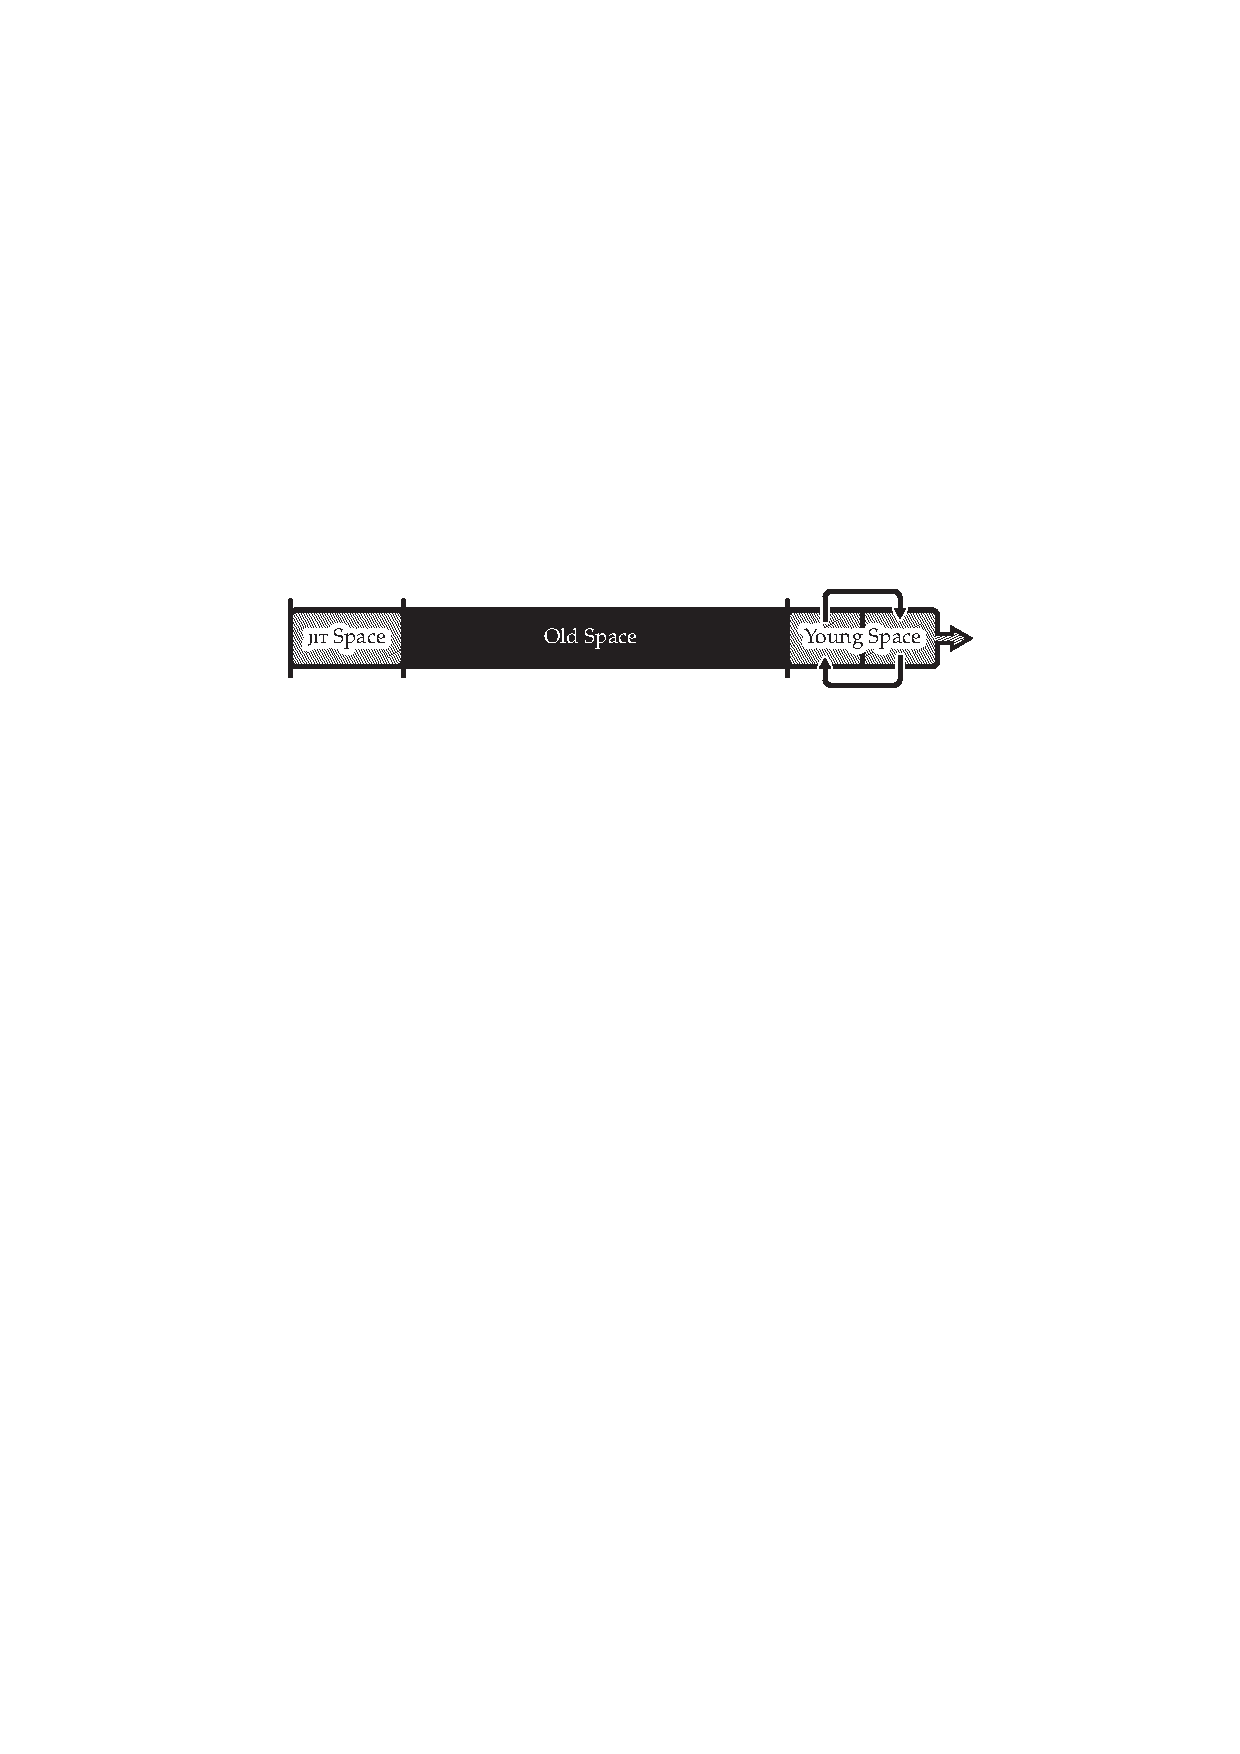
\includegraphics[scale=\imagescale]{cog-memory}
	\caption[\Cog Memory Model Overview]{\Cog Memory Model Overview: Fixed-sized \JIT space, slow changing old space and fast young space.}
	\figlabel{cog-memory}
\end{figure}
%
New objects are allocated in the young space which uses a fast semispace \GC with frequent reclaiming.
Objects that survive a \GC pass move to the old space where infrequent reclaims happen.
Separated from the two memory regions where normal \PH objects reside is the \JIT space dedicated for native code.
In \Cog the \JIT space has its own \GC strategy tailored to native code which is stored in a structure called \ttt{CogMethod}.
Each jitted \PH method has a corresponding \ttt{CogMethod} with native code which resides in the \JIT space.
The \ttt{CogMethod} caches certain information such as the selector or number of arguments.
Again this improves code locality as all the frequently accessed information resides in the \JIT space.
\figref{cog-method} gives an overview of the \ttt{CogMethod}.
We see that additionally to the cached meta information there is relocation information (method map) attached to the \ttt{CogMethod}.
This is used to update object reference, typically to selectors, form the native code in sync with the objects that were moved in a \GC pass.
The same information is also used to update jumps to other native code in the \JIT space if the dedicated \JIT \GC performs a compaction.
%
\begin{figure}[h]
	\centering
	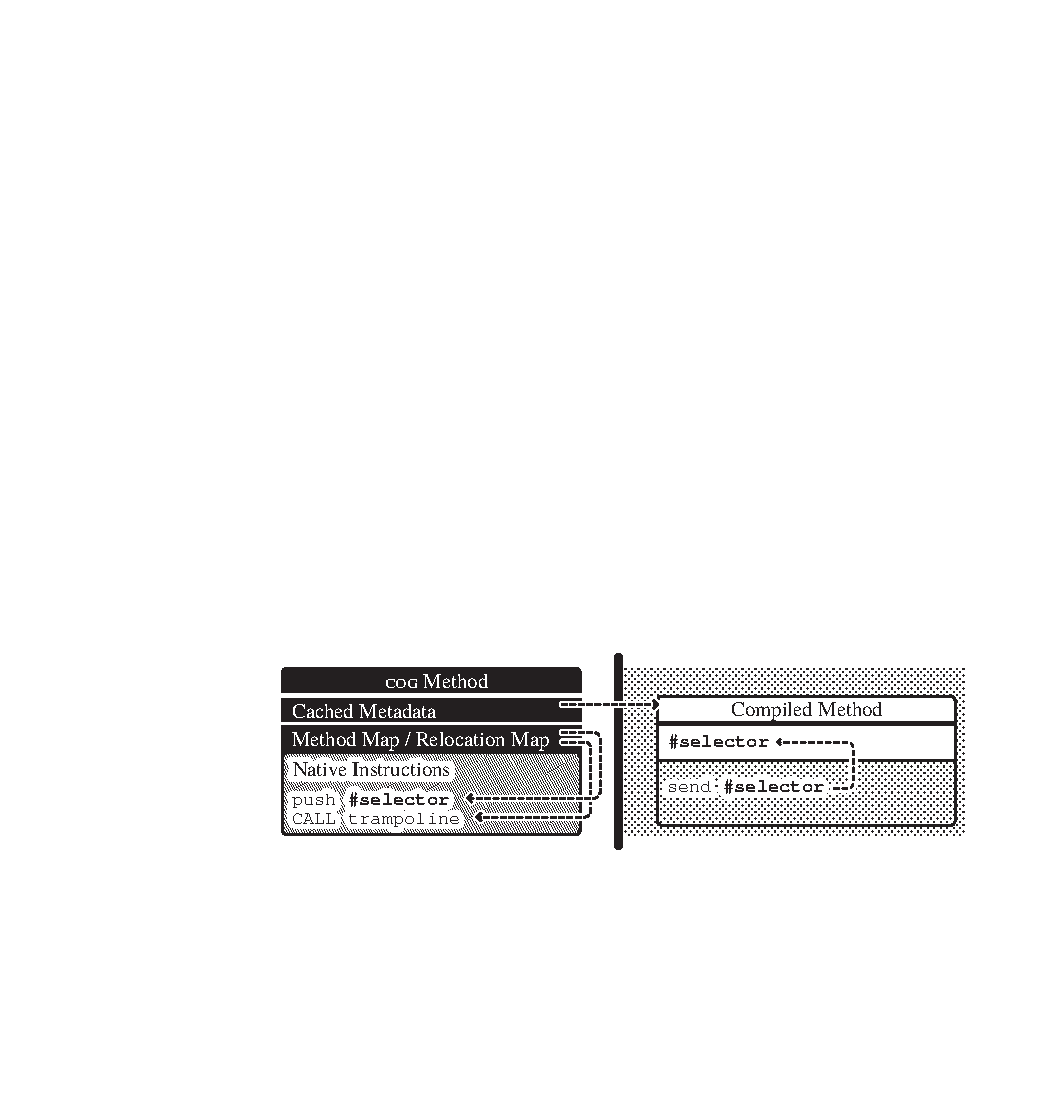
\includegraphics[scale=\imagescale]{cog-method}
	\caption[\Cog Method]{\Cog Method: Compiled method representation at \JIT-level residing in the \JIT memory space.}
	\figlabel{cog-method}
\end{figure}

\noindent So far we explained how \Cog uses native stack mapping for performance reasons and how the basic \JIT compiler works.
The limit the stress on the \CPU cache only the most used methods are jitted.
\Cog uses a hierarchy of inline caches to avoid the costly method lookup and checks if a method is already jitted or not.
Message sends from one jitted method to another hence happen with a very low overhead.
However, due to the limited size of the \JIT space that still means that infrequently used methods are evaluated using the existing bytecode interpreter.
\cb{the previous paragraph might be a bit dense, depending on the knowledge of the reader}



\todo{Step 3: Trampolines to jump back and forth between native activated scheme and bytecode interpreter based approach}\\

%----------------------------------------------------------------------------
\paragraph{Limitations of \VM-level \JIT Compilers}
In the context of \NBJ we separate a \JIT infrastructure into separate parts.
The major part is to have a \VM that uses stack-mapping.
In the case of a bytecode-based interpreter, we assume that the \VM provides routines to switch between a bytecode interpretation context and a low-level native execution context.
With \NBJ we move the \JIT compiler,the part that generates native code at runtime, from the \VM to the image.%, the part that generates native code at runtime, typically from bytecodes.
 Since the \JIT compiler is quite decoupled from the rest of the \JIT infrastructure we believe that a hard-coded static and low-level implementation is not optimal for several reasons:

\begin{itemize}
	\item Optimizing \ST code requires strong interactions with the dynamic environment.
	\item Accessing language-side properties from the \VM-side is hard.
	\item Changing the \JIT compiler requires changes at \VM-level.
	\item The \JIT reimplements primitives for optimization reasons resulting in code duplication.
\end{itemize}

\paragraph{Optimization Limitations for \PH}
In \ST methods tend to be very small and it is considered good practice to delegate behavior to other objects.
This implies that several common optimization techniques for static languages do not work well.
Dynamic method activation does not provide enough context for a static compiler to optimize methods.
Hence after inline caches and register allocation the next optimization technique is inlining.
However, inlining in a dynamic context is difficult and requires hooks at \VM-level to invalidate native code when the language-side changes.
Since in \PH, compiling a method to bytecode is handled completely with language-side code most of the infrastructure to get notified about method changes is already present.

\paragraph{Primitives in the Existing \JIT}
The existing \JIT reimplements the most used primitives at \VM-level.
This guarantees that the \VM stays as long as possible in the \JIT context (see \secref{benzo-jit-interaction} on page~\pageref{sec:benzo-jit-interaction}).
Additionally this enables new performance optimizations that for instance are hard to achieve with standard compliant C code.
A typical example is the integer addition which has to deal with overflow checks and conversion of tagged integers.
In \secref{val-waterfall} we describe how \WF suffers a similar constraint.
\WF manually defines such primitives in terms of native assembler instructions through the language-side \B interface.
\NBJ reuses the same optimized primitives so we rely on a single optimized definition which is shared among all native code libraries.

%----------------------------------------------------------------------------
\subsection{\NBJ Implementation}
\seclabel{val-nabujito-implementation}
%----------------------------------------------------------------------------
\NBJ is an experimental \JIT implementation which replaces the bytecode to native code translation of the existing \JIT infrastructure with a dynamic language-side implementation.
\NBJ is implemented mainly with a visitor strategy over the existing intermediate bytecode representation. 
Additionally we reimplemented vital native routines for the \JIT which are not directly exported by the \VM using \B. 
\cb{not sure if better to put down next to the \JIT limitation paragraphs...}
Nabujito relies on the following \VM-level infrastructure to manage and run native code for any \PH method:

\begin{itemize}[noitemsep,nolistsep]
	\item native stack management,
	\item routines for switching contexts,
	\item \JIT-level memory management for code segments.
\end{itemize}

\noindent The native stack mapping is an implicit requirement for an efficient \JIT.
Since this feature requires deep changes at \VM-level we can not alter or reimplement this at language-side.
However, the routines for switching between \JIT and non-\JIT execution context can be mostly reimplemented at language-side.
We only chose to implement a small subset of them with \B that were directly required for performing message sends.
Some of the helper routines' C-level addresses are easily accessible from language-side using \ttt{dlsym}.
Hence we reuse these for simplicity and only reimplemented the ones that are "hidden".
The last item we reuse, \JIT-level memory management, poses certain problems as we have little to no control over this from language-side.
There is no well-defined interface to interact with the \JIT from language-side in \PH.
However, to properly interact with the \JIT we have to tell it where references to language-side objects are located in the native code.
To overcome this limitation we chose to hack the current \VM to better interact with the \JIT.
More details on this topic follow in the following paragraphs.

\paragraph{\NBJ Dynamic Code Generation}
\NB mainly consists of a visitor over the bytecode-level \IR that is provided by the \PH compiler.
Additionally we reimplemented some of the aforementioned helper routines to switch execution context in the \VM.
The main difficulty of the \NBJ compiler is the missing interface to the \JIT.
For instance we did not have direct control on which methods in \PH are jitted or not, or to force-\JIT a method.
We added one additional primitive to be able to manually trigger \JIT compilation.

For standard methods \NBJ takes the bytecodes and transforms them with a visitor to native code.
It also applies simple optimizations such as creating low-level branches for \PH-level branching operations such as \ttt{ifTrue:}.
Optimizations for additional methods are all implemented flexibly at language-side.
Wherever possible, we reimplement the same behavior as the existing native \JIT compiler.

Eventually the native code is ready and \B attaches it to the existing compiled method.
At this point we benefit from the \JIT integration of \B itself.
As a reminder, we have shown in \secref{benzo-benzo} how \B-enabled methods are treated like normal primitive methods.
The \VM triggers a \B primitive which itself then jumps to the native code attached to the \B-enabled method.
By default the \Cog \JIT can only directly inline the native code for a known set of primitives.
As we have shown in \secref{benzo-jit-interaction} that the \Cog's \JIT was made aware of the special behavior of the \B primitive.
Hence, whenever a \B-enabled method is jitted its native code is directly accessible to the \JIT and inlined.
Thus we essentially remove the overhead of activating \B-enabled methods since we do not have to leave the \JIT execution mode.
As a result we call \B-enabled methods at the same speed as the existing \JIT.


\paragraph{Talking to the \JIT}
After the initial promising progress on building \NBJ on top of \B we soon realized that is does not suffice to just generate the equivalent native code as the \VM internal \JIT.
The first goal was to compile a simple method that just returns a constant integer.
Even at this stage it became apparent that there is a missing interface to the \JIT.
To explain that we have a look at the standard stack frame setup of a jitted method in \Cog shown in \lstref{val-nabujito-cog-frame}.
%
\begin{numstcode}[
	caption={\Cog \JIT Stackframe Setup},
	label={lst:val-nabujito-cog-frame}]{7}
push EBP
mov  EBP, ESP
push 0x1f452b00<CogMethod>
mov  EBX, 0x1f500004<nil>
push EBX
push EBX
\end{numstcode} 
%
After finishing executing these setup instructions the stack frame looks as depicted in \figref{val-nabujito-cog-stack-frame}.
%
\begin{figure}[h]
	\centering
	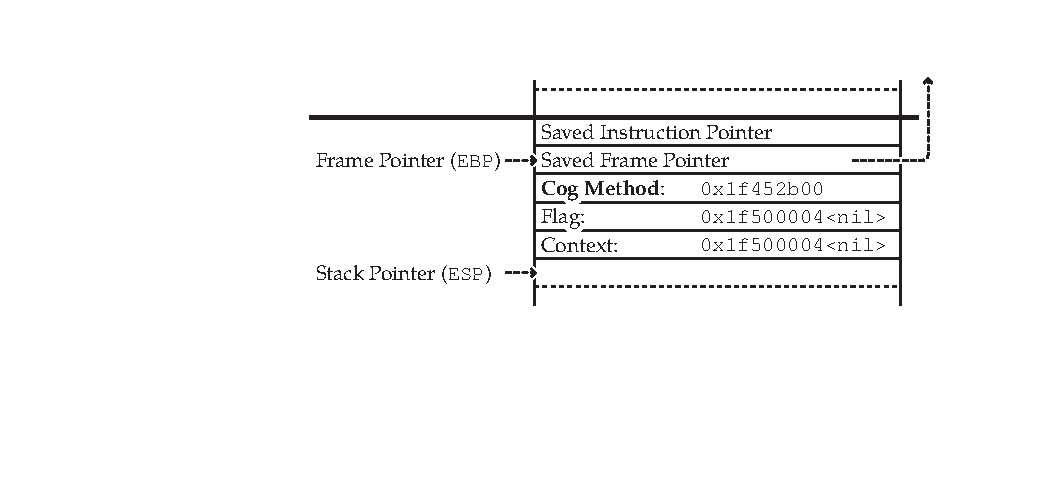
\includegraphics[scale=\imagescale]{cog-stack-frame}
	\caption{\Cog Stack Frame Header}
	\figlabel{val-nabujito-cog-stack-frame}
\end{figure}
%
As we can see there are already two references to \ttt{nil} in the stack frame header.
Already these two references pose a problem in a simple \NBJ setup, but for now we focus on the reference to the \ttt{CogMethod}.
As we explained earlier the \ttt{CogMethod} is a meta object at \JIT-level to make certain information of \PH methods faster accessible.
The \VM currently keeps a pointer to the class, the selector or the number of arguments cached in there.
Having the information there improves locality and make the assembler code required for the frequent querying simpler.
Going back to the native code in \lstref{val-nabujito-cog-frame} we see that we need the final address of the \ttt{CogMethod} for the frame setup.
However, at the moment where \NBJ generates the native code the target method is not yet jitted.
This again implies that the corresponding \ttt{CogMethod} has not yet been allocated by the \JIT.
And since the native code has to be installed in the \JIT we inevitably have to wait for \NBJ to finish compilation, we are stuck.

Instead of directly putting the absolute address of the meta-object in the native code we add a call to a helper routine which will patch the original code on the first activation.
We can do so since we know the following things:
\begin{itemize}[noitemsep,nolistsep]
	\item \ttt{CogMethod}s have a fixed size known upfront,
	\item we know the relative offset of the jitted method's instruction to the start of its \ttt{CogMethod},
	\item we can access the instruction pointer with a helper routine.
\end{itemize}
%
\noindent With this information we modify \NBJ to generate the modified frame setup show in \lstref{val-nabujito-frame-setup}.
%
\begin{numstcode}[
	caption={\NBJ Stack Frame Setup},
	label={lst:val-nabujito-frame-setup}]{7}
push EBP
mov  EBP, ESP

mov  EAX, 0x643d02e<pushCogMethodHelper>
call EAX
\end{numstcode}
%
In the \ttt{pushCogMethodHelper} we access the instruction pointer from where the call happened in the stack frame setup and deduce the start of the \ttt{CogMethod}.
Once the address of the \ttt{CogMethod} is retrieved the \ttt{pushCogMethodHelper} patches the \ttt{MOV} and \ttt{CALL} instruction in the jitted method.
The result is shown in \lstref{val-nabujito-patched-frame-setup}.
%
\begin{numstcode}[
	caption={\NBJ Patched Stack Frame Setup},
	label={lst:val-nabujito-patched-frame-setup}]{7}
push EBP
mov  EBP, ESP

push 0x1f452b00<CogMethod>
nop
\end{numstcode}
%
By using this indirection we circumvent the missing interface to the \JIT.
The helper routine only imposes a one-time overhead, however we slow down the final execution of the \NBJ method by a single \ttt{NOP} instruction.
Yet, looking at the \Cog stack frame in \figref{val-nabujito-cog-stack-frame} we only dealt with finding the reference to the \ttt{CogMethod}.
So far we left out the \GC interaction at \JIT-level, which leads us to the following paragraph.

\paragraph{Overcoming the \GC Missing \VM Interface for the \JIT}

\todo{explain the proplem of object relocation vs. native code}

% -----------------------------------------------------------------------------
\subsection{\NBJ Validation}
\seclabel{val-nabujito-performance}
% -----------------------------------------------------------------------------

\todo{missing intro}

% -----------------------------------------------------------------------------
\subsubsection*{Compilation Time}


The performance evaluation for our \B-based \JIT compiler is focused on the language-side code-generation part.
\NBJ essentially generates the same native code as the \VM-level \JIT, hence there is no performance difference at evaluation time.
However, \NBJ is clearly slower during the warm-up phase.
Compilation of the native instructions will take considerably more time compared to the \VM-level implementation of the same bytecode to assembler transformation.
The cost of transforming the bytecodes to native code at \VM-level can be measured in native instructions, whereas the unit at language-side is bytecodes.
However, we point out again, that this is a one-time overhead.
From the in-production experience of \NB, the \B-based \FFI (see \secref{ffi-evaluation}), we know that these costs amortized, especially for long-term applications.
Instead of focusing on the final performance of the generated code, we present the compilation time compared to the normal \PH bytecode compiler, which also resides at language-side.

\begin{table}[!ht]
    \centering
    \begin{tabular}{rS}
                      & {Compilation Time [ms]} \\\midrule
        \PH Compiler  & 71(1) \\
        \NBJ          & 73(1)
    \end{tabular}
    \caption[\NBJ Compilation Speed]{Compilation efforts of the standard \ST compiler in \PH and \NBJ for the a simple method returning the constant \ttt{nil}.}
    \tablabel{val-nabujito-performance-small}
\end{table}

\noindent In \tabref{val-nabujito-performance-small} we compare the compilation speed of the standard \PH compiler and \NBJ.
We measure the accumulated time spent to compile the method 1000 times.
The average and deviation are taken over 100 runs. 
The \PH compiler takes source code as input and outputs \ST bytecodes.
\NBJ takes bytecodes as input and outputs native code.

We see that in the simple case displayed in \tabref{val-nabujito-performance-small} \NBJ's compilation speed lies within the same range as the standard \ST compiler.
We expect that in the future we apply more low-level optimizations and thus increase the compilation time of \NBJ.
However, we have shown in the performance evaluation for \NB, the \B-based \FFI, in \secref{ffi-evaluation} that even a rather high one-time overhead is quickly amortized.
Furthermore with \ST's image approach the generated native code is persistent over several sessions.
A subsequent restart of the same runtime will not cause the \JIT to nativize the same methods it did during the last launch.
Hence our approach is even valid for short-timed script-like applications as most of the methods will already be available in optimized native code from a previous run.

% -----------------------------------------------------------------------------
\subsubsection*{Per Method Comparison}
\todo{choose simple enough methods that we can compile with nabujito: currently only + works}


% -----------------------------------------------------------------------------
\subsection{Problems}
\seclabel{val-nabujito-problems}
% -----------------------------------------------------------------------------
\paragraph{Hidden \VM Internals}
\todo{backref to patch methods}\\
\todo{maintenance problem: \NBJ harcodes the \VM interaction} \\
\todo{unsuited \VM architecture for a feasible real-world \JIT} \\
\todo{focusing on a future version on SISTA}


\paragraph{Debugging Cycle}
\todo{Missing tools to directly interact with benzo / the real vm} \\
\todo{missing small assembler tests} \\
\todo{reactivate the VM simulator infrastructure} \\
\todo{missing \VM development tools under \PH (mainly disassembler)}

\paragraph{Missing Optimizations}
One major performance optimization missing in both, the original \PH \VM-level \JIT and \NBJ, is inlining. 
By inlining we are able to create methods that are potentially big enough for optimizations.
However, inlining is a difficult task in a highly dynamic language such as \ST or \Self \cite{Cham89a}. 
Efficient inlining can only be performed with sufficient knowledge of the system. 
Accessing this high-level information from within the \VM is cumbersome and requires duplication of language-side reflective features.
The \JIT lives on the same level as the information it needs relying on the already present reflective features of \ST.


% ===========================================================================
\section{Outlook}
% ===========================================================================

\todo{Common problem: missing debugging infrastructure} \\
\todo{\WF and \NBJ share the same problems} \\
\todo{For speed a proper \JIT interface is missing } \\
\todo{SISTA} \\
\todo{better intermediate format (VCPU) from \B}

% ===========================================================================
\section{Summary}
% ===========================================================================


% =============================================================================
% empty version for the main document, where all the chapters are compiled together
\documentclass[a4paper,10pt,twoside]{../includes/ThesisStyle}
\usepackage[utf8]{inputenc}
\usepackage[T1]{fontenc}

\usepackage[left=1.5in,right=1.3in,top=1.1in,bottom=1.1in,includefoot,includehead,headheight=13.6pt]{geometry}\renewcommand{\baselinestretch}{1.05}


% =============================================================================
%\usepackage[sectionbib]{chapterbib}	% Cross-reference package (Natural BiB)
%\usepackage{bibunits}
%\usepackage{natbib}					% Put References at the end of each chapter
\usepackage{algorithm}
\usepackage{alltt}
\usepackage{amsfonts}
\usepackage{amsmath}
\usepackage{amssymb}
\usepackage{cite}
\usepackage{color}
\usepackage{enumerate}
\usepackage{fancyhdr}					% Fancy Header and Footer
\usepackage{graphicx}
\usepackage{ifthen}
\usepackage{latexsym}
\usepackage{multirow}
\usepackage{rotating}					% Sideways of figures & tables
\usepackage{stmaryrd}
\usepackage{subfigure}
\usepackage{url}         
\usepackage{xspace}

\usepackage[a4paper,pagebackref,hyperindex=true]{hyperref}
        

% =============================================================================

% Table of contents for each chapter
\usepackage[nottoc, notlof, notlot]{tocbibind}
\usepackage{minitoc}
\setcounter{minitocdepth}{1}
\mtcindent=15pt

\setcounter{secnumdepth}{3}
\setcounter{tocdepth}{2}
  
% =============================================================================
% Fancy Header Style Options

\pagestyle{fancy}                       % Sets fancy header and footer
\fancyfoot{}                            % Delete current footer settings

%\renewcommand{\chaptermark}[1]{         % Lower Case Chapter marker style
%  \markboth{\chaptername\ \thechapter.\ #1}}{}} %

%\renewcommand{\sectionmark}[1]{         % Lower case Section marker style
%  \markright{\thesection.\ #1}}         %

\fancyhead[LE,RO]{\bfseries\thepage}    % Page number (boldface) in left on even
% pages and right on odd pages
\fancyhead[RE]{\bfseries\nouppercase{\leftmark}}      % Chapter in the right on even pages
\fancyhead[LO]{\bfseries\nouppercase{\rightmark}}     % Section in the left on odd pages

\let\headruleORIG\headrule
\renewcommand{\headrule}{\color{black} \headruleORIG}
\renewcommand{\headrulewidth}{1.0pt}
\usepackage{colortbl}
\arrayrulecolor{black}

\fancypagestyle{plain}{
  \fancyhead{}
  \fancyfoot{}
  \renewcommand{\headrulewidth}{0pt}
}


% =============================================================================
% Clear Header Style on the Last Empty Odd pages
\makeatletter

\def\cleardoublepage{\clearpage\if@twoside \ifodd\c@page\else%
  \hbox{}%
  \thispagestyle{empty}%              % Empty header styles
  \newpage%
  \if@twocolumn\hbox{}\newpage\fi\fi\fi}

\makeatother

\newenvironment{maxime}[1]
{
\vspace*{0cm}
\hfill
\begin{minipage}{0.5\textwidth}%
%\rule[0.5ex]{\textwidth}{0.1mm}\\%
\hrulefill $\:$ {\bf #1}\\
%\vspace*{-0.25cm}
\it 
}%
{%

\hrulefill
\vspace*{0.5cm}%
\end{minipage}
}

\let\minitocORIG\minitoc
\renewcommand{\minitoc}{\minitocORIG \vspace{1.5em}}


\renewcommand{\epsilon}{\varepsilon}

% centered page environment
\newenvironment{vcenterpage}
	{\newpage\vspace*{\fill}\thispagestyle{empty}\renewcommand{\headrulewidth}{0pt}}
	{\vspace*{\fill}}
	
	
% =============================================================================
\newboolean{showcomments}
\setboolean{showcomments}{true}

\ifthenelse{\boolean{showcomments}} {
	\newcommand{\ugh}[1] {\textcolor{red}{\uwave{#1}}}	% please rephrase
	\newcommand{\ins}[1] {\textcolor{blue}{\uline{#1}}}	% please insert
	\newcommand{\del}[1] {\textcolor{red}{\sout{#1}}}	% please delete
	\newcommand{\chg}[2] {								% please change
		\textcolor{red}{\sout{#1}}{\ra}
		\textcolor{blue}{\uline{#2}}}
	\newcommand{\nbc}[3]{								% comment
		{\colorbox{#3}{\bfseries\sffamily\scriptsize\textcolor{white}{#1}}}
		{\textcolor{#3}{\sf\small$\blacktriangleright$\textit{#2}$\blacktriangleleft$}}}

}{
	\newcommand{\ugh}[1]{#1}							% please rephrase
	\newcommand{\ins}[1]{#1}							% please insert
	\newcommand{\del}[1]{}								% please delete
	\newcommand{\chg}[2]{#2}							% please change
	\newcommand{\nbc}[3]{}								% comment
}

% =============================================================================
\usepackage[a4paper,pagebackref,hyperindex=true]{hyperref}


% Links in pdf
\usepackage{color}
\definecolor{linkcol}{rgb}{0.0, 0.0, 0.0} 
\definecolor{citecol}{rgb}{0.0, 0.0, 0.0} 

% Change this to change the informations included in the pdf file
% See hyperref documentation for information on those parameters
\hypersetup {
	bookmarksopen=true,
	pdftitle="Design and Use of Anatomical Atlases for Radiotherapy",
	pdfauthor="Olivier COMMOWICK", 
	pdfsubject="Creation of atlases and atlas based segmentation", %subject of the document
	%pdftoolbar=false, % toolbar hidden
	pdfmenubar=true, %menubar shown
	pdfhighlight=/O, %effect of clicking on a link
	colorlinks=true,
	pdfpagemode=None,
	pdfpagelayout=SinglePage,
	pdffitwindow=true,
	linkcolor=linkcol,
	citecolor=citecol,
	urlcolor=linkcol
}

% =============================================================================
\newcommand{\figlabel}[1]{\label{fig:#1}}
\newcommand{\seclabel}[1]{\label{sec:#1}}
\newcommand{\tablabel}[1]{\label{tab:#1}}

\newcommand{\figref}[1]{Figure~\ref{fig:#1}}
\newcommand{\secref}[1]{Section~\ref{sec:#1}}
\newcommand{\tabref}[1]{Table~\ref{tab:#1}}

\newcommand{\commented}[1]{}

\newcommand{\eg}{\emph{e.g.,}\xspace}
\newcommand{\ie}{\emph{i.e.,}\xspace}


\newcommand\fix[1]{\nb{FIX}{#1}}
\newcommand\todo[1]{\nb{TO DO}{#1}}

% =============================================================================

\graphicspath{{.}{../figures/}}

\begin{document}
% =============================================================================
\chapter{Future Work}
\chaplabel{future}
\minitoc
% =============================================================================
\introduction
% =============================================================================

In \chapref{background} we gave an overview of different concepts of reflection focusing on the main distinction between language-side and \VM-side reflection.
While language-side reflection is very well described in research and rather wide-spread in dynamic languages, the \VM-side counterpart is not.
Compile-time reflection is the center of many popular \VM generation frameworks, but they usually exclude the dynamic reflection aspect of the final binary.
Nevertheless, it is always possible to introspect (structural reflection) the \VM at a very basic level.
Additionally, there are tools like \DTrace which provide a simple way to instrument a binary with little prior setup required.
Thus a limited form of intercession is possible on the binary executable themselves.
However, this still does not make the internal structural information of the \VM accessible that were available at compilation time.
And the restrictions are even more severe when it comes to \VM-level intercession.
It is foreseen for languages to dynamically influe the underlying \VM.

In the course of this thesis we presented tools that try to enter the field of \VM-level reflection -- all based on \B, a common framework to activate native code from language-side.

\WF's dynamic primitives are a first step towards modifying \VM behavior from language-side in a rather controlled way.
By bringing the metacircular \VM sources alive in \PH we connect the former static definition to the running artifact.
Modification happen not by injecting basic native instructions but at high-level by modifying and dynamically compiling primitives.

In contrast to \WF we developed \NBJ, a \JIT compiler prototype, that moves the original \VM component to the language-side.
While \NBJ is defined as language-side compiler using familiar coding patterns, its interaction with the \VM is not clean.
Unlike the plugins and primitives defined by \WF the \JIT generates native code that is heavily depending on the low-level and internal execution model of the \VM.
Unlike \WF \NBJ requires a modified \VM to add a basic interface for manually injecting \JIT code.

In this chapter we present possible solutions and an early prototype \VM that addresses the limitations we encountered while developing \NB, the \B-based \FFI, \WF and \NBJ.
We start by listing possible improvements for the language-side part of the \B infrastructure such as providing a well-defined high-level intermediate format.
This will lead to a description of required \VM-level improvements to make applications such as \WF or \NBJ feasible outside a research context.


% =============================================================================
\section{Background and Related Work}
\seclabel{future-related-work}
\seclabel{future-background}
% =============================================================================
The improvements to the existing infrastructure \B and possible future work is influenced by two research projects we described already in detail in \secref{background-reified-vms}: the \P \VM and the \Klein \VM.
For this chapter we present a small summary of these two metacircular \VMs with the focus on two things: their own limitations compare to \B and their influence on improvements and future work.


% -----------------------------------------------------------------------------
\subsection{\P \VM}
% -----------------------------------------------------------------------------

The \P \VM \cite{Verw11a} presented in \secref{background-pinocchio} is a direct predecessor of the work presented in this thesis.
The knowledge gained while participating on \P had a great influence on the development direction of \B and its applications.

Unlike \PH running on the \Cog \VM the \P research \VM has no bytecode interpreter.
The only execution base is native code which is directly generated by the language-side compiler.
At the current stage of development \P has not yet support for a separate image as in \PH.
The runtime image is currently defined by the bootstrap process where classes, objects and methods are exported into binary images and linked together with a primitive kernel to a final executable.

\paragraph{Going Native}
We took from \P that language-side native code generation is not more complex than generating bytecodes.
Instead we directly embrace the native world.
This means that in the core \P already uses many concepts that are only introduced by the \JIT in the \Cog \VM.
Hence, \P does no longer distinct between \JIT mode and interpreter mode.
Here the gain for \P are twofold: we could boost the performance of the language-runtime and simplify the design by not needing a dual compilation pipeline for the \JIT and the bytecode.

\paragraph{Going Meta}
Even so \P directly uses native code as core execution mode we avoided to directly write native code if possible.
For instance the method lookup in \Cog is statically implemented at \VM-side using \Slang.
We described in \secref{background-pinocchio} in detail how \P uses language-side code instead for the lookup.
Using the combination of low-level code to flatten out meta recursion we still have full language-side control over the lookup while maintaining good performance.

\paragraph{Missing Low-level Reification}
The most obvious shortcoming of \P was the lack of its own garbage collector.
Instead of investing time into a separate well-defined \GC \P relies on the conservative \urlfootnote{Boehm \GC}{http://www.hpl.hp.com/personal/Hans_Boehm/gc/} built for C programs.
The Boehm \GC is sufficiently fast to run \P as a prototype, however, due to its generic nature it is not as efficient as a specific \GC.
However, \P lacked the necessary reification at level of the object layout to properly implement a \GC.
All the notion about the object layout in memory are hard-coded in the compiler in several places.

\paragraph{Missing C Independence:}
The second negative point of \P is its dependence from C.
During the course of the \P development we greatly reduced the quantity of C code.
However, for simplicity we relied on a small C Kernel for the complete bootstrap of the language.
Additionally some crucial primitives that required system calls were implemented in C.

% -----------------------------------------------------------------------------
\subsection{MIST: A C-less \ST Implementation}
% -----------------------------------------------------------------------------
\urlfootnote{\MIST}{http://mist-project.org/} is another prototype \ST \VM that follows similar goals as the \P \VM.
It not longer uses bytecode interpreter but only relies on native code.
However, it goes one step further than \P by not relying on any C-based infrastructure.
\MIST implements its own linker to build the final executable.
And unlike \P it does not require kernel primitives written in C.
\MIST brings its own implementation to directly perform system calls from within the language.


% -----------------------------------------------------------------------------
\subsection{\Klein \VM}
% -----------------------------------------------------------------------------
\todo{refer to \secref{background-klein}}\\
\todo{read again} \\
\todo{\VM and language written in the same language} \\
\todo{unified model for runtime and compile time} \\
\todo{\VM-level reflection since there is only a single code base}\\
\todo{Responsive developement: no C++ / C compilation wait process involved}\\
\todo{Cmopared to \B radical break with the existing system, no fluent development} \\
\todo{Even though \B is capable, \Klein is much more} \\
\todo{much less hard-coded \VM level objects} \\

\todo{Fancy Debugging}

% -----------------------------------------------------------------------------
\subsection{\Maxine \VM}
% -----------------------------------------------------------------------------
\todo{refer to \secref{background-maxine} \cite{Wimm13a}}\\
\todo{inspector overview} \\
\todo{fluent navigation from low-level code to high-level inspectors}

\Maxine is a metacircular \Java \VM focused on an efficient developer experience.
The \Maxine \VM stands out as it truly focuses on productivity and developer interaction.
\Maxine uses abstract and high-level representations of \VM-level concepts and consistently exposes them throughout the development process.
Inspectors at multiple abstraction levels are readily available while debugging, giving insights to the complete \VM state.
Compared to \Maxine, \WF currently lacks the debugging tools which would enable a truly seamless interaction with the low-level world.
However, \Maxine focuses on \Java, a language with inferior reflective capabilities compared to \PH.
Hence the live interaction with the \VM is only presented in the development phase and not exposed to the language-side.
\Maxine would be an excellent candidate to implement our approach for \Java.


% =============================================================================


% =============================================================================
%\newpage
\section{Language-side Improvements}
\seclabel{future-language}
% =============================================================================
In this section we present the suggestion for improvements related mostly tied to the language-side part of \B.
Most of the solutions have been presented in the separate chapters of \B in \secref{benzo-problems}, \NB \FFI in \secref{ffi-problems} and the \B application prototypes (\secref{validation-waterfall-problems} and \secref{validation-nabujito-problems}).

% -----------------------------------------------------------------------------
\subsection{Improved Domain Specific Inspectors}
% -----------------------------------------------------------------------------
Domain specific inspectors are important for an efficient development as we pointed out in \secref{reification-inspectors}.
Similar to the \JIT approach we have to optimize the frequent tasks during development and provide a seamless integration.
This becomes even more important when working with low-level code and data that does not come with existing first-class structures.
We noticed that using \B for \NBJ and \WF that it is more convenient to rely on an existing low-level text-based debugger such as \ttt{gdb} to inspect C-level structures.

We have seen excellent use of inspectors in the \VM development of the \Cog \VM itself.
The original simulator supports inspecting objects in simulated raw memory.
\Cog added additional inspectors including disassembled instructions for the \JIT development.
However, with the recent changes the advanced simulator does not yet run in \PH and requires attention.

Lately we have seen a very similar approach for the \Maxine research \VM \cite{Wimm13a}.
It provides excellent low-level debugging interaction, switching seamlessly between low-level assembler views and high-level object inspectors.
We believe that it is an imperative requirement for a \VM development \IDE to support customizable inspectors that span from high-level to low-level.
Even though existing C-focused \IDEs provide more and more support for integrated inspectors the \VM domain has different needs.
C inspectors are tailored towards fixed-sized objects whose types can be statically inferred.
Whereas, for \VMs we only have a handful types of object layouts and the real type is only implicitly available.
For instance in certain \VMs the class is encoded in the header of an object instead of a simple full pointer to the class object.
This means that a minor interpretation pass is necessary to retrieve such information.
Which is why most C-focused \IDEs are only partially sufficient for an efficient \VM development.


% -----------------------------------------------------------------------------
\subsection{Barrier-free Low-level Interaction}
% -----------------------------------------------------------------------------
Shifting from \VM development to the final language-runtime we see a similar issue when it comes to tools that span abstraction levels.
It is not directly possible to inspect low-level objects from language-side.
Focusing the on the \B architecture what comes closes to inspecting low-level objects is the \ttt{struct} support for the \NB \FFI library described in \secref{ffi-newtypes}.
We already use this approach for the \NBJ project to inspect \VM internal meta objects for debugging purposes.
It is important to note that giving access to the \VM internal objects is not permitted in most languages.
The previously mentioned \VM generation frameworks usually have first-class objects for all the \VM internal objects or provide mirror-like facilities to access objects from raw memory.
Usually, none of this structural information survives the \VM compilation phase.
Essentially this leaves the final \VM binary with little or no means for introspection. Of course the same restrictions apply then for language-side tools like \B that want to interact with the \VM internals.

\paragraph{Customized \VM \MOP}
We have seen in \secref{validation-nabujito-problems} for \NBJ that the only way to circumvent such issues is by creating modified \VMs which enable specific interaction points.
There are other \PH-based research projects \cite{??} that took the same path and created a modified \VM.
We, believe that with an extended low-level \MOP the focus for research projects could shift from the \VM to the language-side.
The final extreme is to have a system that works like the described \Klein \VM where there is no longer a clear distinction of what is \VM-level and what is language-side.

\paragraph{Anticipated Debugging}
For \B we have more modest intermediate goals.
The major drawback for a seamless developer experience is the lack of a dedicate low-level debugging infrastructure.
At this point, \B developers have to rely on 3rd-party C-centric tools for debugging.
Hence, a developer has to decide upfront at which abstraction level the debugging should occur.
Either at high-level without the possibility to deal with low-level errors, or at low-level losing all the inspection capabilities.
Besides the shortcomings that either side of the decision will bring, already the fact that the debugging direction has to be anticipated is inappropriate.

We outlined in \secref{benzo-problems-debugging} already several ways to improve the current debugging situation for \B.
The most important focus is on reducing the cases where the programmer has to anticipate the debugging tool.
Since we have to deal with two very distinct abstraction levels we can not only rely on a pure language-side solution to provide different debuggers \cite{Towards a Moldable Debugger}.
The major problem is the serious implications of a low-level error.
Unlike user-level errors they are not well-defined or even contained.
It is astonishingly simple to corrupt the \VM memory while writing low-level code and thus breaking any contract with the \VM code.
However, it is more common to access protected memory due to a wrongly dereferenced pointer.
Hence, the \B should focus on this most common bug by following the solution outlined in \figref{benzo-debugger}.
%
\begin{figure}[h]
	\centering
	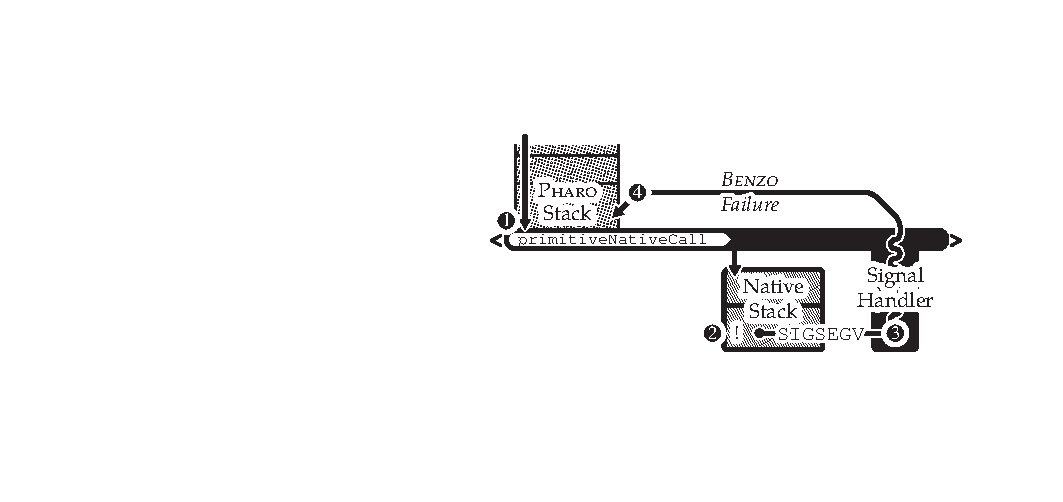
\includegraphics[scale=\imagescale]{benzo-debugger}
	\caption{\B Debugger Outline}
	\figlabel{benzo-debugger}
\end{figure}
%
\begin{enumerate}
	\item Standard \PH method activating a \B-enabled method through the \ttt{primitiveNativeCall} primitive.
	\item Native code causing a memory access violation (for example \ttt{SIGSEV}) which can not be handled by \PH directly.
	\item Low-level signal handler is activated by the operating system and tries to walk back the native stack up to the \ttt{primitiveNativeCall} activation.
	\item After successfully finding the \ttt{primitiveNativeCall} the signal handler sends a \B failure back to \PH.
\end{enumerate}

\paragraph{Barrier-free Debugging}
After proposing a solution to improve \B's bug recovery behavior we immediately encounter a second problem.
How do we debug low-level code?
With the aforementioned solution we are able to recover from certain low-level errors and signal them properly at language-side.
In a \ST-like environment the debugger will pop up on the location causing the error and thus allowing a programmer to inspect stack and variables.
To provide the same facility for \B we have to plug into the existing low-level debugging utilities such as \ttt{ptrace} to enable stepping over native instructions.
The following \figref{benzo-crossover-debugger} outlines the basics of a debugger that crosses the high-level / low-level barrier.
%
\begin{figure}[h]
	\centering
	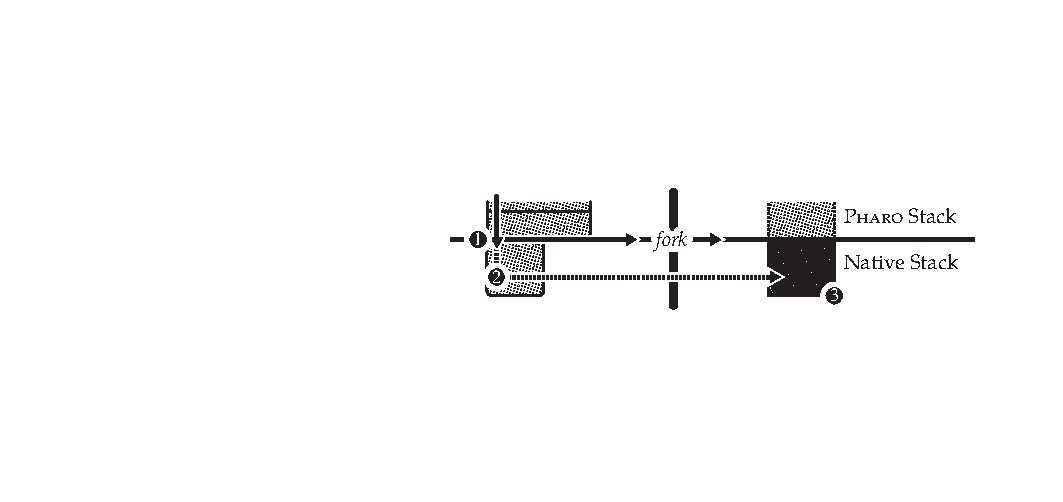
\includegraphics[scale=\imagescale]{benzo-crossover-debugger}
	\caption{\B Crossover Debugger Outline}
	\figlabel{benzo-crossover-debugger}
\end{figure}
%
\begin{enumerate}
	\item Point where a \B initiates a native call and the debugger switches from a high-level \PH stack to the low-level native stack.
To properly use low-level debugging tools we fork the complete \VM process.
	\item The low-level debugger in \PH switches the underlying debugging interface.
Instead of directly interacting with first-class \PH context we communicate to the the forked process with tools like \ttt{ptrace}.
	\item The forked process is updated according to the actions initiated from the \PH side.
\end{enumerate}

\noindent The outlined debugger will not work in certain cases where the native code directly interacts with the outer image.
The forked debugger process provides security from the main \PH image by isolating it.
However, for many \B applications such as the \FFI implementation this limitation would not apply.

\cb{more?}

% -----------------------------------------------------------------------------
\subsection{Virtual \CPU an Assembler \DSL}
% -----------------------------------------------------------------------------
\B uses \AsmJIT as assembler backend which is currently limited to x86 instruction set.
This choice is aligned with \PH main development branches for the most common operating systems.
However, this excludes mobile devices which currently focus on \ARM-based architectures.
To support this new architecture we have to extend the assembler backend in \AsmJIT.
The changes for \B-based applications such as the \NB \FFI are more severe.
Essentially most low-level code has to be replicated for each new platform.
A better solution is to use an intermediate format for all the low-level code which is then compiled for each platform specifically.

\todo{\ASM code is too low-level: \NB lacks expressiveness} \\
\todo{see \secref{benzo-problems-platform-independence}} \\
\todo{\ASM is hard to debug directly: very un \PH-ish, we need direct feedback}

\paragraph{A Low-level Intermediate Format}
\todo{change a bit to make the copy}
\VCPU is based on a \TAC to simplify the adoption of optimizations such as \SSA.
These \TAC instruction take the following form:
%
\begin{stcode}{}
result := argument1 OP argument2
\end{stcode}
%
There are three operands involved, \ttt{result}, \ttt{argument1} and \ttt{argument2}, from which the name of this instruction format originates.
Based on this assumption, each standard \VCPU instruction returns a temporary variable which can be used for further operations.
The following code example outlines the basic usage of \VCPU:
%
\begin{stcode}[
	label={lst:benzo-problem-vcpu}, 
	caption={Basic \VCPU Example}
]{}
Benzo vcpu x86 generate: [ :asm | | temp1 temp2 |
	temp1 := asm memoryAt: 16r12345.
	temp2 := asm uint: 2.
	asm return: temp1 + temp1 ]
\end{stcode}
%
Which corresponds to the same functionality expressed in the following x86 instructions:
%
\begin{stcode}{}
Benzo x86 generate: [ :asm |
	asm mov: 16r12345 ptr to: asm EAX.
	asm add: asm EAX with: 2.
	asm return ]
\end{stcode}

%%\todo{Design overview/flow figure with backends} \\
\todo{inject high-level instructions} \\
\todo{explain the difference to explicit code like \ASM by having a different backends}

\paragraph{\VCPU Testing and Debugging}
\todo{\VCPU interpreter} \\
\todo{tracer backend for code generation} \\
\todo{Native Simluator for the specific backends} \\
\todo{Requires mapping from native instruction to the \VCPU instructions}


\paragraph{\VCPU Optimizations}
\todo{Optimizations required for \B-based applications can be shared} \\

To get to the final native instructions the \VCPU infrastructure compiles the high-level instructions to the specific backend.
The current compiler is divided into the following passes:
%
\begin{itemize}[noitemsep]
\item Platform Specific Transformation
\item Register Allocation
\item Superfluous Assignment Remover
\item Platform Specific Assembler
\end{itemize}



\todo{Current State of the Implementation} \\
\todo{Support new Platforms} \\
\todo{Indirect support for simluation and thus better debugging}


% =============================================================================
\section{\VM-level Improvements}
\seclabel{future-vm}
% =============================================================================
\todo{Introduction: Lanugage-side is not enough} \\
\todo{Need to get a obstacle-free VM} \\
\todo{List of requirements for a new VM Infrastructure} \\ 
\todo{Small comparison against the current solution we have with COG} \\
\todo{Follow the \Klein approach}


% -----------------------------------------------------------------------------
\subsection{VM-level Reification}
% -----------------------------------------------------------------------------
\todo{Resulting from the first law of Inspectors, all VM-level objects are reified} \\
\todo{List of typical objects that don't have a reification in COG} \\
\todo{List advantages}\\
\todo{make concepts explicit and first-class} \\
\todo{limit the use of raw memory access and string-based programming} \\

% -----------------------------------------------------------------------------
\subsection{Runtime Reification / Dual Objects}
% -----------------------------------------------------------------------------
\todo{Reuse the same objects for the bootstrap and at runtime inspectors/mirrors} \\
\todo{goes further than the sheer compile-time reification} \\
\todo{accessible from language-side => leads to the following MOP}

% -----------------------------------------------------------------------------
\subsection{Mate Object Model and Runtime MOP}
% -----------------------------------------------------------------------------
\todo{consequence of the runtime reification of the VM introspection => intercession}\\
\todo{Rough Overview of all the Objects currently present in Mate (UMLish)}

% -----------------------------------------------------------------------------
\subsection{Be Native}
% -----------------------------------------------------------------------------
\todo{out of the intercession capabilities follows that we need native support at runtime (see \B)}\\
\todo{that means we need to have decent / better infrasrtucture for native code}\\
\todo{need to be able to achieve what \NBJ didn't manage: compile native methods and hand them over to the \VM}\\
\todo{step towards our implementation in \Mate}


% =============================================================================
\section{\Mate a Reflective \VM Prototype}
\seclabel{mate}
% =============================================================================

\begin{figure*}[h]
	\begin{adjustwidth}{-10.0in}{-10.0in}
		\centering
		
\includegraphics[width=1.02\textwidth]{mate-logo}
	\end{adjustwidth}
\end{figure*}

\todo{introduction: protoype based on the conclusions presented in the previous sections}\\
\todo{for reasearch mainly but possible long term solution to our \VM problems}

% -----------------------------------------------------------------------------
\subsection{Mate Compiler Outline}
\seclabel{future-mate-compiler}
% -----------------------------------------------------------------------------
\todo{Small Intro: Reuse the bootstrap infrastrucutre at runtime (FFI, JIT...)}

\begin{figure}[H]
\centering
	\includegraphics[width=\textwidth]{mate-compilation-toolchain}
\end{figure}

% -----------------------------------------------------------------------------
\subsection{Mate Bootstrap Outline}
\todo{Small Intro: Why Bootstrap and how to use the reified objects}\\
\todo{Compare to Pinocchio (manual approach)}\\
\todo{Work in Progress: Envision the trace-based Bootstrap}


% -----------------------------------------------------------------------------
\subsection{Mate Towards Complete Reflection}
\todo{list possible paths between the 4 quadrants of reflection}\\
\todo{usecase: dynamic gc change}\\
\todo{usecase: dynamic object format influence}\\
\todo{usecase: optimize partial behavior reflection (immutability, proxies)}\\

% =============================================================================
\section{SISTA: Language-side Adaptive Recompilation}
% =============================================================================

\todo{do we put this in a separate section?}\\
\todo{related to \NBJ, but more real-world approach}

% =============================================================================
\section{Reflective Future}
% =============================================================================
% NEW concepts
\todo{Check with GUIDO} \\
\todo{List 3 to 4 different Examples entering the 4th quadrant:}

% -----------------------------------------------------------------------------
\subsection{Accessible VM Components}
% -----------------------------------------------------------------------------
\todo{Access GC Statistics} \\
\todo{Access JIT Statistics for Type Annotations / Tooling}

% -----------------------------------------------------------------------------
\subsection{Interchangeable VM Components}
% -----------------------------------------------------------------------------
\todo{Change GC strategy} \\
\todo{Change JIT Strategy}

% -----------------------------------------------------------------------------
\subsection{Interchangeable Language Semantics}
% -----------------------------------------------------------------------------
\todo{Up to which extent can this be supported?} \\
\todo{Related to VM MOP: How much should be changeable? When?}


% -----------------------------------------------------------------------------
\subsection{Efficient Reflection}
% -----------------------------------------------------------------------------
\todo{Reflectivity at VM-level} \\
\todo{Flatten but don't freeze Reflection/Abstraction}


% =============================================================================
\section{Summary}
% =============================================================================

\todo{a lot of work on the engineering level to get a \VM with reflective properties}\\
\todo{- limited resources focused on maintaining the current infrastructure} \\
\todo{for research we have already sufficient tools at hand to experiment} \\
\todo{- outline some stuff for guido} \\
\todo{possiblity to split up off tools to be used by \PH} \\
\todo{- VCPU IR} \\
\todo{- improved FFI}


% =============================================================================
% empty version for the main document, where all the chapters are compiled together
\documentclass[a4paper,10pt,twoside]{../includes/ThesisStyle}
\usepackage[utf8]{inputenc}
\usepackage[T1]{fontenc}

\usepackage[left=1.5in,right=1.3in,top=1.1in,bottom=1.1in,includefoot,includehead,headheight=13.6pt]{geometry}\renewcommand{\baselinestretch}{1.05}


% =============================================================================
%\usepackage[sectionbib]{chapterbib}	% Cross-reference package (Natural BiB)
%\usepackage{bibunits}
%\usepackage{natbib}					% Put References at the end of each chapter
\usepackage{algorithm}
\usepackage{alltt}
\usepackage{amsfonts}
\usepackage{amsmath}
\usepackage{amssymb}
\usepackage{cite}
\usepackage{color}
\usepackage{enumerate}
\usepackage{fancyhdr}					% Fancy Header and Footer
\usepackage{graphicx}
\usepackage{ifthen}
\usepackage{latexsym}
\usepackage{multirow}
\usepackage{rotating}					% Sideways of figures & tables
\usepackage{stmaryrd}
\usepackage{subfigure}
\usepackage{url}         
\usepackage{xspace}

\usepackage[a4paper,pagebackref,hyperindex=true]{hyperref}
        

% =============================================================================

% Table of contents for each chapter
\usepackage[nottoc, notlof, notlot]{tocbibind}
\usepackage{minitoc}
\setcounter{minitocdepth}{1}
\mtcindent=15pt

\setcounter{secnumdepth}{3}
\setcounter{tocdepth}{2}
  
% =============================================================================
% Fancy Header Style Options

\pagestyle{fancy}                       % Sets fancy header and footer
\fancyfoot{}                            % Delete current footer settings

%\renewcommand{\chaptermark}[1]{         % Lower Case Chapter marker style
%  \markboth{\chaptername\ \thechapter.\ #1}}{}} %

%\renewcommand{\sectionmark}[1]{         % Lower case Section marker style
%  \markright{\thesection.\ #1}}         %

\fancyhead[LE,RO]{\bfseries\thepage}    % Page number (boldface) in left on even
% pages and right on odd pages
\fancyhead[RE]{\bfseries\nouppercase{\leftmark}}      % Chapter in the right on even pages
\fancyhead[LO]{\bfseries\nouppercase{\rightmark}}     % Section in the left on odd pages

\let\headruleORIG\headrule
\renewcommand{\headrule}{\color{black} \headruleORIG}
\renewcommand{\headrulewidth}{1.0pt}
\usepackage{colortbl}
\arrayrulecolor{black}

\fancypagestyle{plain}{
  \fancyhead{}
  \fancyfoot{}
  \renewcommand{\headrulewidth}{0pt}
}


% =============================================================================
% Clear Header Style on the Last Empty Odd pages
\makeatletter

\def\cleardoublepage{\clearpage\if@twoside \ifodd\c@page\else%
  \hbox{}%
  \thispagestyle{empty}%              % Empty header styles
  \newpage%
  \if@twocolumn\hbox{}\newpage\fi\fi\fi}

\makeatother

\newenvironment{maxime}[1]
{
\vspace*{0cm}
\hfill
\begin{minipage}{0.5\textwidth}%
%\rule[0.5ex]{\textwidth}{0.1mm}\\%
\hrulefill $\:$ {\bf #1}\\
%\vspace*{-0.25cm}
\it 
}%
{%

\hrulefill
\vspace*{0.5cm}%
\end{minipage}
}

\let\minitocORIG\minitoc
\renewcommand{\minitoc}{\minitocORIG \vspace{1.5em}}


\renewcommand{\epsilon}{\varepsilon}

% centered page environment
\newenvironment{vcenterpage}
	{\newpage\vspace*{\fill}\thispagestyle{empty}\renewcommand{\headrulewidth}{0pt}}
	{\vspace*{\fill}}
	
	
% =============================================================================
\newboolean{showcomments}
\setboolean{showcomments}{true}

\ifthenelse{\boolean{showcomments}} {
	\newcommand{\ugh}[1] {\textcolor{red}{\uwave{#1}}}	% please rephrase
	\newcommand{\ins}[1] {\textcolor{blue}{\uline{#1}}}	% please insert
	\newcommand{\del}[1] {\textcolor{red}{\sout{#1}}}	% please delete
	\newcommand{\chg}[2] {								% please change
		\textcolor{red}{\sout{#1}}{\ra}
		\textcolor{blue}{\uline{#2}}}
	\newcommand{\nbc}[3]{								% comment
		{\colorbox{#3}{\bfseries\sffamily\scriptsize\textcolor{white}{#1}}}
		{\textcolor{#3}{\sf\small$\blacktriangleright$\textit{#2}$\blacktriangleleft$}}}

}{
	\newcommand{\ugh}[1]{#1}							% please rephrase
	\newcommand{\ins}[1]{#1}							% please insert
	\newcommand{\del}[1]{}								% please delete
	\newcommand{\chg}[2]{#2}							% please change
	\newcommand{\nbc}[3]{}								% comment
}

% =============================================================================
\usepackage[a4paper,pagebackref,hyperindex=true]{hyperref}


% Links in pdf
\usepackage{color}
\definecolor{linkcol}{rgb}{0.0, 0.0, 0.0} 
\definecolor{citecol}{rgb}{0.0, 0.0, 0.0} 

% Change this to change the informations included in the pdf file
% See hyperref documentation for information on those parameters
\hypersetup {
	bookmarksopen=true,
	pdftitle="Design and Use of Anatomical Atlases for Radiotherapy",
	pdfauthor="Olivier COMMOWICK", 
	pdfsubject="Creation of atlases and atlas based segmentation", %subject of the document
	%pdftoolbar=false, % toolbar hidden
	pdfmenubar=true, %menubar shown
	pdfhighlight=/O, %effect of clicking on a link
	colorlinks=true,
	pdfpagemode=None,
	pdfpagelayout=SinglePage,
	pdffitwindow=true,
	linkcolor=linkcol,
	citecolor=citecol,
	urlcolor=linkcol
}

% =============================================================================
\newcommand{\figlabel}[1]{\label{fig:#1}}
\newcommand{\seclabel}[1]{\label{sec:#1}}
\newcommand{\tablabel}[1]{\label{tab:#1}}

\newcommand{\figref}[1]{Figure~\ref{fig:#1}}
\newcommand{\secref}[1]{Section~\ref{sec:#1}}
\newcommand{\tabref}[1]{Table~\ref{tab:#1}}

\newcommand{\commented}[1]{}

\newcommand{\eg}{\emph{e.g.,}\xspace}
\newcommand{\ie}{\emph{i.e.,}\xspace}


\newcommand\fix[1]{\nb{FIX}{#1}}
\newcommand\todo[1]{\nb{TO DO}{#1}}

% =============================================================================

\graphicspath{{.}{../figures/}}

\begin{document}
% =============================================================================
\chapter{Conclusion}
\chaplabel{conclusion}
\minitoc
% =============================================================================
\introduction 

\todo{}

% =============================================================================
\section{Contributions}
% =============================================================================
\todo{detection of \VM level reflectivity => reification?} \\
%\todo{identification of tools that cross vm boundaries} \\
\todo{identification of partial solution of these tools using benzo} \\
\todo{identification of the restrictions of a benzo-based tool}
The main contributions of this thesis are:
\begin{enumerate}
	\item Description of the properties of an open and reflective language runtime.
	\item Implementation of 3 main software artifacts to show the feasibility of an open \VM.
	\item A road map for the future, bottom-up implementation of an open language runtime.
\end{enumerate}

\todo{some prose text}

% =============================================================================
\section{Published Papers}
% =============================================================================

% -----------------------------------------------------------------------------
\subsection*{\href{http://dx.doi.org/10.1145/2048066.2048138}{Flexible object layouts: enabling lightweight language extensions by intercepting slot access}}
% -----------------------------------------------------------------------------

This paper contributed to \chapref{reification}.
Slots and Layouts as described in this paper are used in \PH 3.0 and newer.
The original implementation presented in this paper was implemented in an older \PH 1.0 image and was ported to \PH 3.0 in 2013.

\begin{description}
	\item[Abstract:] \emph{
Programming idioms, design patterns and application libraries often introduce cumbersome and repetitive boilerplate code to a software system.
Language extensions and external \textsc{dsl}s (domain specific languages) are sometimes introduced to reduce the need for boilerplate code, but they also complicate the system by introducing the need for language dialects and inter-language mediation.
To address this, we propose to extend the structural reflective model of the language with object layouts, layout scopes and slots.
Based on the new reflective language model we can 1) provide behavioral hooks to object layouts that are triggered when the fields of an object are accessed and 2) simplify the implementation of state-related language extensions such as stateful traits.
By doing this we show how many idiomatic use cases that normally require boilerplate code can be more effectively supported.
We present an implementation in \ST, and illustrate its usage through a series of extended examples.}

	\item[Authors:] Toon Verwaest, Camillo Bruni, David Gurtner, Adrian Lienhard and Oscar Nierstrasz. 
	\item[Revenue:] In Onward! 2011, Reno/Tahoe, Nevada, USA, 2011.
	\item[URL:] \url{http://dx.doi.org/10.1145/2048066.2048138}
\end{description}

% -----------------------------------------------------------------------------
\subsection*{\href{http://hal.inria.fr/hal-00840781}{Language-side Foreign Function Interfaces with \NB}}
% -----------------------------------------------------------------------------

This paper served as the basis for \chapref{ffi} and discusses the \B-based \FFI implementation \NB in detail.
\NB is used in production in the \PH 2.0 and newer.

\begin{description}
	\item[Abstract:] \emph{
		Foreign-Function-Interfaces (\FFIs) are a prerequisite for close system integration of a high-level language.
		With \FFIs the high-level environment interacts with low-level functions allowing for a unique combination of features.
		This duality has a strong impact on the implementation of the \FFI: it has to be flexible and fast at the same time.
		We propose \NB a language-side approach to \FFIs that only requires minimal changes to the \VM.
		\NB directly creates specific native code at language-side and thus combines the flexibility of a language-side library with the performance of a native plugin.}

	\item[Authors:] Camillo Bruni, Luc Fabresse, Stéphane Ducasse and Igor Stasenko. 
	\item[Revenue:] In International Workshop on \ST Technologies, Annecy, France, 2013.
	\item[URL:] \url{http://hal.inria.fr/hal-00840781}
\end{description}



% =============================================================================
\section{Software Artifacts}
% =============================================================================
\todo{make proper subsections/paragraphs} \\
\todo{make sure there is a proper link (arxiv.org... figshare) for each artifact}
\begin{description}
	\item[Collaboration on First-class Layouts and Slots:]
		In a collaboration with To\-on Verwaest (\SCG, Switzerland) we built a first implementation of first-class layouts and slots in a \ST system \cite{Verw11a}.
		In Collaboration with Martin Días (\RMoD, \INRIA) this initial version was ported to \PH and is now used in the current release candidate \urlfootnote{\PH 3.0}{http://files.pharo.org/image/30}.

	\item[\AsmJIT 64-bit Assembler:]
		To reuse the original research compilation pipeline built with \P \cite{Verw10a, Brun11a} a 64-bit extension was necessary to the initial \urlfootnote{\AsmJIT implementation for \PH}{http://smalltalkhub.com/\#!/~Pharo/AsmJit}.
		The extension is included in the current stable \urlfootnote{\PH release 2.0}{http://files.pharo.org/image/20}.

	\item[Collaboration on the \WF Dynamic Primitives:]
		We collaborated on the \WF Dynamic Primitive compiler together with Guido Chari (\UBA, Argentina), which resulted in paper currently under submission\cite{Char13a}.
		The implementation is a prototype and is not used in production.

	\item[Collaboration on the Mate \VM Prototype:]
		In collaboration with Guido Cha\-ri (\UBA, Argentina), Javier Pímas (\UBA, Argentina) and Clement Bera (\RMoD, \INRIA) several stages of a prototype \VM were built.
		The implementation mainly follows the concept of an dynamic language runtime which controls every aspect at language-side.
		The current language runtime is in a early prototype phase that allows us to explore new \VM and language concepts, however it is not production ready.
		Guido Chari will further explore new concepts of Mate in his Ph.D.
		Clement Bera, after finishing his engineering contract at \RMoD, will continue to work as a Ph.D. on the same system.

	\item[\VirtualCPU Compilation Toolchain:]
		In collaboration with Clement Bera (\RMoD, \INRIA) and Igor Stasenko (\RMoD, \INRIA) we built a prototype compilation toolchain based on the original work of Pinocchio.
		The current implementation is a working prototype.
		Plans exist to integrate a streamlined version into \PH to server as a platform independent backend to our \B-based \FFI implementation used in \PH.

	\item[\NBJ Language-side \JIT Compiler:]
		As a third case study for the \B framework we implemented a language-side \JIT compiler. 
		The current implementation is a prototype that is capable of directly transforming simple methods to executable code.
		Unlike its \VM-level counterpart it is based as a simple visitor over the intermediate bytecode format already present at language-side.

	\item[Inspector Framework for \PH:] 
		An important part of reifying concepts is the possibility to inspect and manipulate these objects.
		We wrote a new inspector framework which is used in the latest \PH release.
		It allows to quickly define new views on domain objects, an indispensable requirement for interacting with complex data objects.
		Next to the everyday usage in \PH it is actively used for the Mate \VM prototype where we need transparent access to internal structures of the \VM.

	\item[Command Line Test Interface for \PH:]
		In order to perform continuous integration in a maintainable fashion we developed a new modular command line interface for \PH. 
		It is used in production on the \urlfootnote{\PH build server}{http://ci.inria.fr/pharo/} alongside with simple \urlfootnote{installer scripts}{http://get.pharo.org/}.
\end{description}


% =============================================================================
\section{Future Work}
% =============================================================================
\todo{Sync Problem section of each chapter} \\
\todo{- Benzo Improvements} \\
\todo{- VM Improvements (Mate)} \\
\todo{- New Reflection}


% =============================================================================
% empty version for the main document, where all the chapters are compiled together


% =============================================================================
\appendix
%\include{appendix/def}
% =============================================================================

\bibliographystyle{include/cami}
\bibliography{local}

% =============================================================================
\include{chapter/cv}
\thispagestyle{empty}
% =============================================================================
\end{document}